%%%%%%%%%%%%%%%%%%%%%%%%%%%%%%%%%%%%%%%%%%%%%%%%%
%%%
%%% Auteur : Stéphane Péchard - stephane.pechard@univ-nantes.fr
%%% Fichier : phd.tex - ma thèse (version finale)
%%% Version : 0.1
%%% Date : 2006/03/27 (début)
%%%
%%%%%%%%%%%%%%%%%%%%%%%%%%%%%%%%%%%%%%%%%%%%%%%%%

\RequirePackage[final]{optional}
% note		affichage des notes en bas de page
% nofinal	enlève les trucs de la version finale
% final		ajoute tous les flonflons pour la version finale


%%%%%%%%%%%%%%%%%%%%%%%%%%%%%%%%%%%%%%%%%%%%%%%%%
%%% Déclaration
%%%%%%%%%%%%%%%%%%%%%%%%%%%%%%%%%%%%%%%%%%%%%%%%%
\documentclass[a4paper,frenchb,pdftex,11pt,twoside,openright]{book} %\raggedbottom% version finale
%%%%%%%%%%%%%%%%%%%%%%%%%%%%%%%%%%%%%%%%%%%%%%%%%
%%% Bidouillages
%%%%%%%%%%%%%%%%%%%%%%%%%%%%%%%%%%%%%%%%%%%%%%%%%
\makeatletter

%% pour pallier au problème des overfull hbox dans la table des matières
\renewcommand{\@pnumwidth}{2em}

%% pour pallier au problème de niveau des algos
% \providecommand{\toclevel@algorithm}{0}

%% supression et remise des warnings (pour virer ceux de fourier notamment)
\let\@font@warningori\@font@warning
\newcommand\shutup{\def\@font@warning##1{}}
\newcommand\youcanspeak{\let\@font@warning\@font@warningori}


%% logos LaTeX dans la bonne police :-)
%%% From File: ltlogos.dtx
\def\myTeX{T\kern-.1667em\lower.4ex\hbox{E}\kern-.1emX\@}
\DeclareRobustCommand{\myLaTeX}{L\kern-.25em%
        {\sbox\z@ T%
         \vbox to\ht\z@{\hbox{\check@mathfonts
                              \fontsize\sf@size\z@
                              \math@fontsfalse\selectfont
                              A}%
                        \vss}%
        }%
        \kern-.15em%
        \myTeX}
\DeclareRobustCommand{\myLaTeXe}{\mbox{\m@th
  \if b\expandafter\@car\f@series\@nil\boldmath\fi
  \myLaTeX\kern.15em2$_{\textstyle\varepsilon}$}}


%% copies de sauvegarde du titre et de la date
\let\Title\@title
\let\Date\@date


%% page d'entrée, redéfinition de maketitle pour ne pas en faire une titlepage
\renewcommand\maketitle{%
  \cleardoublepage
  \thispagestyle{empty}
  \let\footnotesize\small
  \let\footnoterule\relax
%   \let \footnote \thanks
  \null\vfil
  \vskip 60\p@
  \begin{center}%
    {\LARGE \@title \par}%
    \vskip 3em%
    {\large
     \lineskip .75em%
      \begin{tabular}[t]{c}%
        \@author
      \end{tabular}\par}%
      \vskip 1.5em%
    {\large \@date \par}%       % Set date in \large size.
  \end{center}\par
  \@thanks
  \vfil\null
  \clearpage
%   \end{titlepage}%
  \setcounter{footnote}{0}%
  \global\let\thanks\relax
  \global\let\maketitle\relax
  \global\let\@thanks\@empty
  \global\let\@author\@empty
  \global\let\@date\@empty
  \global\let\@title\@empty
  \global\let\title\relax
  \global\let\author\relax
  \global\let\date\relax
  \global\let\and\relax
}


%%%%%%%%%%%%%%%%%%%%%%%%%%%%%%%%%%%%%%%%%%%%%%%%%%%%%%
%%% hack pour avoir la continuité dans la numérotation
%%%%%%%%%%%%%%%%%%%%%%%%%%%%%%%%%%%%%%%%%%%%%%%%%%%%%%
% sauvegarde du \pagenumbering habituel
\let\pagenumberingori\pagenumbering

% redéfinit \pagenumbering comme d'habitude sauf que le compteur \c@page n'est pas remis à zéro
\newcommand*\newpagenumbering{%
   \gdef\pagenumbering##1{%
     \gdef\thepage{\csname @##1\endcsname \c@page}%
   }
}

% remet \pagenumbering à son comportement par défaut (on ne sait jamais)
\newcommand\restorepagenumbering{%
   \global\let\pagenumbering\pagenumberingori
}

% sauvegarde du \mainmatter normal
\let\mainmatterori\mainmatter

% C'est bon, on peut y aller
\renewcommand\mainmatter{%
   % cassage en règle du \pagenumbering
   \newpagenumbering
   % appel du \mainmatter normal qui va se faire blouser lorsqu'il appellera \pagenumbering. hé hé hé !
   \mainmatterori
   % on remet \pagenumbering en place. Ni vu, ni connu.
   \restorepagenumbering
}
%%%%%%%%%%%%%%%%%%%%%%%%%%%%%%%%%%%%%%%%%%%%%%%%%

\makeatother

 % bidouillages en tout genre


% \includeonly{a-base}
% introduction, 0-contextePbTVHD, 1-testsub, 2-HDContexteQual, 3-evalImpactSysDegsurQual, 4-metriques, 5-eval, 6-modQualVid, 7-modClassif, a-base, b-transfoCouleur, conclusion, publications

%%%%%%%%%%%%%%%%%%%%%%%%%%%%%%%%%%%%%%%%%%%%%%%%%
%%% Packages
%%%%%%%%%%%%%%%%%%%%%%%%%%%%%%%%%%%%%%%%%%%%%%%%%
%% Packages de programmation
% \usepackage{ifpdf}
% \usepackage{etex}
% \usepackage{calc}
% \usepackage{ifthen}
% \usepackage{ifmtarg}

%% Packages primordiaux
\usepackage[utf8]{inputenc}													% codage d'entrée (tout le document en dépend)
\usepackage[T1]{fontenc}													% codage de la fonte
% \shutup \usepackage{fourier} \youcanspeak									% pour les maths (avec suppression des warnings) !! À mettre avant lmodern ou garamond !!
% \usepackage{agaramondpro}													% la famille de fonte dépend du codage
\usepackage{lmodern}
% \usepackage[kerning=true,babel=true]{microtype}
\usepackage{textcomp}														% dépend de la famille de la fonte
\usepackage{setspace}														% interlignage
\usepackage[pdftex, headheight=15.91pt]{geometry}		% taille du papier (peut dépendre de l'interlignage par l'option lines=... , textheight=22cm
\usepackage{fancyhdr}														% dépend du papier
% \usepackage{floatrow}

%% Zone floue
% math
\usepackage{amsmath}   														% math
\usepackage{amssymb}														% symboles
\usepackage{amsfonts}														% fontes
\usepackage{array}															% tableaux en mode math
\usepackage{multirow}														% pour les tableaux
\usepackage{mathtools}														% amélioration de amsmath
\usepackage{stmaryrd}
% déco
\usepackage{lettrine}														% lettrine en tête de chapitre
\renewcommand{\LettrineFontHook}{\color[gray]{0.6}} 						% normalement le même gris que les numéros de quotchap
\usepackage{tikz}															% jolis graphiques ;-)
\usetikzlibrary{arrows,patterns,plotmarks,backgrounds,shapes,shadows}		% librairies
% layout
\usepackage[center, labelsep=endash]{caption}								% avant subfig
\usepackage{subfig}															% plusieurs figures en une seule (remplace subfigure)
\usepackage{pdfpages}														% inclusion de pdf
\usepackage{titlesec}
\usepackage{wrapfig}														% pour insérer des images au long
\usepackage[nottoc]{tocbibind}
\usepackage{colortbl}
\usepackage{booktabs}
\setlength{\heavyrulewidth }{0.2em}
% \usepackage{titletoc}
% \usepackage{makeidx}
% \usepackage{index}
% \usepackage{float}
% \usepackage{fancyvrb}

% utile
% \usepackage{shorttoc}											% table des matières réduite TODO problème avec titletoc ?
\usepackage{lastpage}											% permet de connaitre le numéro de la dernière page
% \usepackage{fancybox}											% des boiboites
\usepackage{eurosym}											% \eurologo (de fourier)
% \usepackage{listings}											% affichage de code
% \usepackage{lipsum}
% \usepackage{verbatim}
% \usepackage{url}
\usepackage[utopia]{quotchap}									% affiche une citation à chaque chapitre (change aussi l'allure de l'en-tête de chapitre)
% \renewcommand{\chapnumfont}{\usefont{LY1}{AGaramondPro}{b}{n}\fontsize{100}{130}\selectfont\color{chaptergrey}}



%% nomenclature (liste des symboles)
% \usepackage[intoc, french, noprefix]{nomencl}
% \renewcommand{\nomname}{Système de notation}
% \renewcommand{\nompreamble}{Voici le système de notation utilisé dans ce document.}
%
% \renewcommand{\nomgroup}[1]{%
% \item[]\hspace*{-\leftmargin}%
% \rule[2pt]{0.45\linewidth}{1pt}%
% \hfill
% \ifthenelse{\equal{#1}{S}}{\textbf{Symboles}}
% {\ifthenelse{\equal{#1}{I}}{\textbf{Indices}}{}}
% \hfill
% \rule[2pt]{0.45\linewidth}{1pt}}
%
% \makenomenclature

%% babel et trucs de langue
% \usepackage[autolanguage]{numprint}
\usepackage[english]{babel}
\usepackage[babel]{csquotes}
\MakeAutoQuote{«}{»}

% infos pour partout
\newcommand{\montitre}{Qualité d'usage en télévision haute définition : évaluations subjectives et métriques objectives}
\newcommand{\datesoutenance}{2 octobre 2008}


%% hyperref et trucs pdf (avec ifpdf mais ne marche plus on dirait)
\usepackage{graphicx}  % Graphiques internes et externes
\usepackage{pstricks}
% \usepackage{thumbpdf}
\usepackage{pdflscape}
\usepackage[pdftex, hyperindex, plainpages=false, pdfpagelabels, pagebackref, colorlinks=false, hypertexnames=false]{hyperref}

\hypersetup{
	pdftitle={\montitre},
	pdfauthor={Stéphane Péchard},
	pdfsubject={La télévision haute définition (TVHD) est le nouveau système de diffusion sensé apporter une plus grande immersion de l'observateur dans l'action et une qualité d'usage supérieure à celle de la télévision standard (TVSD). Afin de remplir ces exigences, les diffuseurs ont besoin de techniques de mesure de qualité adaptées. Le premier objectif de cette thèse est de nous éclairer sur l'impact de la transition de la TVSD vers la TVHD sur la qualité visuelle. Le second est de proposer des métriques objectives de qualité adaptées à la TVHD. Nous avons tout d'abord étudié plusieurs aspects de la qualité visuelle dans ce contexte. Cela nous a notamment permis de sélectionner une méthodologie d'évaluation subjective de la qualité pour constituer une base de séquences dégradées par un codage H.264. Puis, nous avons proposé une méthodologie d'évaluation de l'impact d'un système dégradant sur la qualité visuelle. Elle est utilisée dans les trois critères objectifs de qualité présentés par la suite. Elle fournit au premier une analyse du contenu permettant de modéliser la qualité visuelle d'une séquence. Le second critère cumule des fonctions de gêne locales en une note de qualité globale grâce à des modèles validés par la méthodologie. Le dernier exploite la notion de tubes spatio-temporels introduits par la méthodologie. Des caractéristiques y sont mesurées pour les séquences de référence et dégradée. Le cumul des différences entre ces caractéristiques fournit une note de qualité finale. Alors que le second critère n'offre pas de résultats convaincants, les deux autres permettent une prédiction des notes subjectives plus performante que celle de deux critères connus de la littérature.},
	pdfkeywords={télévision haute définition, qualité subjective de la vidéo, codage H.264},
	pdfcreator={\LaTeXe}
% 	pdfproducer={Stéphane Péchard}
}
\usepackage[all]{hypcap}


%%% après hyperref
%% glossaire
% \usepackage[number=none, hypertoc=true, style=list]{glossary} % style=altlist !!!! à placer après hyperref !!!!
% \makeglossary

%%%%%%%%%%%%%%%%%%%%%%%%%%%%%%%%%%%%%%%%%%%%%%%%%
%%% Commandes
%%%%%%%%%%%%%%%%%%%%%%%%%%%%%%%%%%%%%%%%%%%%%%%%%
\newcommand{\ornementChapitre}{\begin{center}\begin{Large}\textorn{2}\end{Large}\end{center}}

%% centrage des colonnes sur plusieurs lignes
\renewcommand\multirowsetup{\centering}

%% création d'un type de colonne centrée de largeur 1.5
\newcolumntype{D}{>{\centering}p{1.5cm}}

%% notes dans la marge
\newcommand{\note}[1]{\marginpar{%
  \vskip-\baselineskip %raise the marginpar a bit
  \raggedright\footnotesize
  \color{red}{\itshape\hrule\smallskip#1}\par\smallskip\hrule}}
\newcommand{\nonotes}{\renewcommand{\note}[1]{}}

%% strong %%
\DeclareRobustCommand{\strong}[1]{%
\textbf{#1}%
}

%% dédicace %%
\DeclareRobustCommand{\dedicace}[1]{%
\clearemptydoublepage
\thispagestyle{empty}
\vspace*{\stretch{1}}\par
{\begin{flushright}\emph{#1}\end{flushright}\par}
\vspace*{\stretch{2}}
}

%% sur-paragraphe (ligne entre deux groupes de paragraphes) %%
\DeclareRobustCommand{\surparagraph}{%
\par\medskip
}

%% raccourcis %%
\newcommand\avc{H.264}
\newcommand\ituCC{ITU-R BT.500-11~\cite{itu-bt500-11}}
\newcommand\ituNfDx{ITU-T P.910~\cite{itu-bt910}}


%%%%%%%%%%%%%%%%%%%%%%%%%%%%%%%%%%%%%%%%%%%%%%%%%
%%% Paramétrages du document
%%%%%%%%%%%%%%%%%%%%%%%%%%%%%%%%%%%%%%%%%%%%%%%%%
%% url dans la même police que le reste
\urlstyle{rm}

%% profondeur de la table des matières
\setcounter{tocdepth}{2}
% \setcounter{secnumdepth}{8}

% on définit l'interligne pour tout le document
\onehalfspacing

% modification de la table des matières -- options titletoc
\usepackage{titletoc}

\titlecontents{part}												% label concerné
[3pc]																	% espace à la marge gauche
{\addvspace{1.5pc}\filcenter\hrule height 1pt \Large{\textbf{Partie}}~}		% formatage global du label (avant)
{\Large\textbf}														% quand il y a un numéro
{\Large\textbf}														% quand il n'y en a pas
{}																		% séparateur (\titlerule*[1pc]{.}) et numéro de la page (\contentspage)
[\hrule height 1pt\addvspace{.5pc}]					% ce qui se passe après


%% redéfinition des labels (tableaux, figures, etc.) % voir french.cfg
\addto\captionsfrench{\def\figurename{Figure}}
\addto\captionsfrench{\def\tablename{Tableau}}
\addto\captionsfrench{\def\listfigurename{Table des illustrations}}

%% définition des en-têtes et pieds de page
\pagestyle{fancy}
\fancyhf{} % on efface tout
\fancyhead[RO]{\nouppercase{\emph{\rightmark}}}
\fancyhead[LE]{\nouppercase{\emph{\leftmark}}}
\fancyfoot[RO,LE]{\ifthenelse{\value{page}=42}{\strong{--~\reflectbox{\thepage}~--}}{\strong{--~\thepage~--}}} % h2g2 style
\fancypagestyle{plain}{ % pour les pages de chapitre
\fancyhf{} % on efface tout
\fancyfoot[RO,LE]{\ifthenelse{\value{page}=42}{\strong{--~\reflectbox{\thepage}~--}}{\strong{--~\thepage~--}}} % h2g2 style
\renewcommand{\headrulewidth}{0pt}}

%% on enlève le pied et l'en-tête d'une page paire vide
\let\origdoublepage\cleardoublepage
\newcommand{\clearemptydoublepage}{%
  \clearpage
  {\pagestyle{empty}\origdoublepage}%
}
\let\cleardoublepage\clearemptydoublepage


%%%%%%%%%%%%%%%%%%%%%%%%%%%%%%%%%%%%%%%%%%%%%%%%%
%%% On attaque le vif du sujet
%%%%%%%%%%%%%%%%%%%%%%%%%%%%%%%%%%%%%%%%%%%%%%%%%
\title{Qualité d'usage en télévision haute définition : \\évaluations subjectives et métriques objectives}
\author{Stéphane Péchard}
\date{\datesoutenance}

\begin{document}
\selectlanguage{frenchb} % on est en français

%%%%%%%%%%%%%%%%%%%%%%%%%%%%%%%%%%%%%%%%%%%%%%%%%
%%%
%%% Auteur : Stéphane Péchard - stephane.pechard@univ-nantes.fr
%%% Fichier : tikzPhD.tex - fichier contenant les styles tikz
%%% Version : 0.1
%%% Date : 2007/06/20
%%%
%%%%%%%%%%%%%%%%%%%%%%%%%%%%%%%%%%%%%%%%%%%%%%%%%

% rectangle bleu aux coins arrondis pour les actions
\tikzstyle{action} = [
draw,
rectangle,
top color=white,
bottom color=blue!30,
text centered,
rounded corners=2mm,
style=loose background,
drop shadow]

% flèche à une direction
\tikzstyle{fleche} = [
draw,
-latex']

% boite pour les légendes
\tikzstyle{legende} = [
draw,
rectangle,
fill=yellow!20,
text centered,
rounded corners=2mm]

 % éléments de tikz
%%%%%%%%%%%%%%%%%%%%%%%%%%%%%%%%%%%%%%%%%%%%%%%%%
%%% %% commandes mathit %% % TODO : à mettre dans un fichier (celui-là ?)
%%%%%%%%%%%%%%%%%%%%%%%%%%%%%%%%%%%%%%%%%%%%%%%%%

\newcommand\HD{\mathit{HD}}


\newcommand\ACrCr{\mathit{ACr_1Cr_2}}
% \newcommand\CC{\mathit{CC}}
\newcommand\Cb{\mathit{Cb}}
\newcommand\Cr{\mathit{Cr}}
\newcommand\CONTRASTE{\mathit{CONTRASTE}}
% \newcommand\covar{\mathit{covar}}
% \newcommand\DSSIM{\mathit{DSSIM}}
\newcommand\HISTO{\mathit{HISTO}}
\newcommand\HV{\mathit{HV}}
\newcommand\IC{\text{IC}}
% \newcommand\ID{\mathit{ID}}
\newcommand\LMS{\mathit{LMS}}
% \newcommand\maxIT{\mathit{max}}
\newcommand\minIT{\mathit{min}}
% \newcommand\Md{\mathit{Md}}
\newcommand\MS{\text{MS}}
\newcommand\MSP{\text{MSP}}
\newcommand\MOS{\mathit{MOS}}
\newcommand\MOSp{\mathit{MOSp}}
\newcommand\DMOS{\mathit{DMOS}}
\newcommand\Dcent{DMOS$_{\text{100}}$}
\newcommand\DcentOpt{DMOS$^\textit{opt}_{\text{100}}$}
% \newcommand\MV{\mathit{MV}}
\newcommand\NO{\text{NO}}
\newcommand\RGB{\mathit{RGB}}
\newcommand\RGBlum{\mathit{RGBlum}}
% \newcommand\RMSE{\mathit{RMSE}}
\newcommand\SI{\mathit{SI}}
\newcommand\SIT{\mathit{SIT}}
% \newcommand\SMVB{\mathit{SMVB}}
% \newcommand\SMVH{\mathit{SMVH}}
% \newcommand\SSIM{\mathit{SSIM}}
\newcommand\Sobel{\mathit{Sobel}}
\newcommand\TI{\mathit{TI}}
\newcommand\YCbCr{\mathit{YCbCr}}
 % définition d'objets
\nonotes % on s'assure qu'on a rien laisser qui traine
%%%%%%%%%%%%%%%%%%%%%%%%%%%%%%%%%%%%%%%%%%%%%%%%%
%%%
%%% Auteur : Stéphane Péchard - stephane.pechard@univ-nantes.fr
%%% Fichier : glossaire.tex - le glossaire de ma thèse
%%% Version : 0.1
%%% Date : 2007/05/13
%%%
%%%%%%%%%%%%%%%%%%%%%%%%%%%%%%%%%%%%%%%%%%%%%%%%%
% makeindex -s gglo -o phdFinal.gls phdFinal.glo

\glossary{name=ACR,
description=Absolute Category Rating}
\glossary{name=AVC,
description=Advanced video coding}
\glossary{name=CIF,
description=Common intermediate format}
\glossary{name=CRT,
description=Cathode ray tube}
\glossary{name=DMOS,
description=Differential mean opinion score}
\glossary{name=DSCQS,
description=Double stimulus continuous quality scale}
\glossary{name=DSIS,
description=Double stimulus impairment scale}
\glossary{name=EBU,
description=European Broadcasting Union}
\glossary{name=GOP,
description=Group of picture}
\glossary{name=HDTV,
description=High definition television}
\glossary{name=ips,
description=images par seconde}
\glossary{name=ITU,
description=International Telecommunication Union}
\glossary{name=ITU-T,
description=International Telecommunication Union -- Telecommunication Standardisation Sector}
\glossary{name=ISO,
description=International organisation for standardisation}
\glossary{name=LCD,
description=Liquid crystal display}
\glossary{name=Mbps,
description=Megabit par seconde}
\glossary{name=MOS,
description=Mean opinion score}
\glossary{name=MPEG,
description=Moving picture experts group}
\glossary{name=MTBF,
description=Mean time between failure}
\glossary{name=MUSHRA,
description=Multiple stimuli with hidden reference and anchor}
\glossary{name=NTSC,
description=National television system committee}
\glossary{name=PAL,
description=Phase alternating line}
\glossary{name=PDP,
description=Plasma display panel}
\glossary{name=PLUGE,
description=Picture line up generating equipment}
\glossary{name=PSNR,
description=Peak signal-to-noise ratio}
\glossary{name=QCIF,
description=Quarter common intermediate format}
\glossary{name=QVGA,
description=Quarter video graphics array}
\glossary{name=RGB,
description=red-green-blue}
\glossary{name=SAMVIQ,
description=Subjective assessment methodology for video quality}
\glossary{name=SCACJ,
description=Stimulus comparison adjectival categorical judgement}
\glossary{name=SDSCE,
description=Simultaneous double stimulus for continuous evaluation}
\glossary{name=SSCQE,
description=Single stimulus continuous quality evaluation}
\glossary{name=SVH,
description=Système visuel humain}
\glossary{name=TNT,
description=Télévision numérique terrestre}
\glossary{name=TVHD,
description=Télévision haute définition}
\glossary{name=TVSD,
description=Télévision standard}
\glossary{name=UTI,
description=Union internationale des télécommunications}
\glossary{name=VGA,
description=Video graphics array}

 % les entrées du glossaire


%%%%%%%%%%%%%%%%%%%%%%%%%%%%%%%%%%%%%%%%%%%%%%%%%
%%% avant-propos (numérotation romaine)
%%%%%%%%%%%%%%%%%%%%%%%%%%%%%%%%%%%%%%%%%%%%%%%%%
\frontmatter

%% page de garde
%%%%%%%%%%%%%%%%%%%%%%%%%%%%%%%%%%%%%%%%%%%%%%%%%%%%%%%%%%%%%%%%%%
% page de garde : Université de Nantes
% EDSTIM
\begin{titlepage}
\thispagestyle{empty}

\begin{center}
\strong{%
\Large{%
Université de Nantes\\
École doctorale\\
« Sciences et technologies de l'information et des mathématiques »}}

\vspace{.5cm}

\large{Année 2008}

\vspace{.5cm}

\strong{\Large{Thèse de doctorat de l'université de Nantes}}

Spécialité : automatique et informatique appliquée

\vspace{.5cm}

\emph{présentée et soutenue publiquement par}

\vspace{.5cm}

\strong{\Large{Stéphane Péchard}}

\vspace{.5cm}

\emph{le 2 octobre 2008}

\emph{à l'École polytechnique de l'université de Nantes}

\vspace{1cm}

\huge{Qualité d'usage en télévision haute définition : \\évaluations subjectives et métriques objectives}

\vspace{1cm}

\strong{\large Jury}
\end{center}

\begin{tabular}{lll} % TODO à améliorer : pourquoi pas les 2 ? en tout cas si une seule : les etablissements
Rapporteurs
	& M. François-Xavier Coudoux 			& \emph{Professeur, université de Valenciennes}\\
	& M. Michel Jourlin						& \emph{Professeur, université de Saint-Étienne}\\
Examinateurs
	& M. Joseph Ronsin						& \emph{Professeur, INSA Rennes}\\
	& Mme	Sheila Hemami					& \emph{Professor, Cornell University, États-Unis}\\
	& Mme Patricia Ladret					& \emph{Maître de conférences, Polytech'Grenoble}\\
	& M. Dominique Barba 					& \emph{Professeur émérite, Polytech'Nantes}\\
	& M. Patrick Le Callet 					& \emph{Professeur, Polytech'Nantes}\\
Membre invité
	& M. Ricardo Pastrana-Vidal 			& \emph{Ingénieur, France Télécom R\&D, Rennes}\\
\end{tabular}

\vspace{.5cm}

\hrule

\vspace{.2cm}

\noindent Directeur de thèse : Dominique Barba\\
Co-encadrant : Patrick Le Callet\\
Institut de recherche en communications et cybernétique de Nantes \hspace{\stretch{1}} N\degre ED 503--004
\end{titlepage}


%% page de titre
\maketitle

%% dédicace
\dedicace{à Lilou, Victor et Gael\\à Éloïse}

%% remerciements
\begin{savequote}[12pc]
Une âme délicate est gênée de savoir qu'on lui doit des remerciements, une âme grossière, de savoir qu'elle en doit.
\qauthor{Friedrich Nietzsche}
\end{savequote}
\chapter*{Remerciements}\markboth{Remerciements}{Remerciements}
L'écriture d'une page de remerciements semble anodine après avoir écrit, corrigé et validé un document comme celui-ci. Pourtant, il n'est jamais évident de revenir sur quatre années comme celles que je viens de passer, de n'oublier personne et de trouver les mots justes pour communiquer une gratitude sincère. De nombreux noms viennent en tête, dont certains semblent bien lointains déjà. Les visages et les souvenirs sont aussi importants que le travail effectué, mais une seule page leur est dédiée ici.

\bigskip

Évidemment, et en tout premier lieu, ce travail n'aurait pu être possible sans mes encadrants Dominique Barba et Patrick Le Callet. Merci à eux pour leur aide, leur patience et leurs encouragements infléchis pendant quatre ans. Merci également à MM. Coudoux et Jourlin d'avoir accepté la tâche de relire mon manuscrit et de rapporter ma thèse. Merci aussi aux membres du jury d'avoir accepté d'en faire partie.

\bigskip

Les deux années centrales furent marquées par le projet HD4U et ses participants à mes côtés. Merci à Mathieu, Arnaud et Romuald pour leur précieux support au développement. Nous n'attendons plus que la soutenance de Sylvain pour clore véritablement :-). L'accomplissement d'une thèse va bien pourtant au-delà d'un projet et c'est toute l'équipe IVC que je tiens à remercier. Notamment, merci à Nicolas pour ses nombreux conseils technico-typologico-informatiques. Je finirai par une pensée à tous les futurs docteurs : bon courage !

\bigskip

D'un point de vue plus personnel, il est évident que le support de personnes plus proches est essentiel. Merci à mes parents, ma famille et leurs p'tits loups énergisants ! Merci à Pierrick pour avoir eu le courage de me demander quel était mon sujet à chaque fois que l'on se voyait, c'est-à-dire trop peu souvent ! Merci à mes amis dont je vais pouvoir profiter un peu plus désormais. Merci enfin et surtout à Éloïse pour avoir été là, tout simplement.

\bigskip

Et merci à tous les observateurs d'être venu participer !
 % TODO

%% diverses tables
\tableofcontents

%%%%%%%%%%%%%%%%%%%%%%%%%%%%%%%%%%%%%%%%%%%%%%%%%
%%% corps du document (numérotation arabe)
%%%%%%%%%%%%%%%%%%%%%%%%%%%%%%%%%%%%%%%%%%%%%%%%%
\mainmatter

%%% introduction
%%%%%%%%%%%%%%%%%%%%%%%%%%%%%%%%%%%%%%%%%%%%%%%%%
%%%
%%% Auteur : Stéphane Péchard - stephane.pechard@univ-nantes.fr
%%% Fichier : introduction.tex - introduction générale de la thèse
%%% Version : 0.1
%%% Date : 2007/11/26
%%%
%%%%%%%%%%%%%%%%%%%%%%%%%%%%%%%%%%%%%%%%%%%%%%%%%

%%%%%%%%%%%%%%%%%%%%%%%%%%%%%%%%%%%%%%%%%%%%%%%%%
% citation
%%%%%%%%%%%%%%%%%%%%%%%%%%%%%%%%%%%%%%%%%%%%%%%%%
% \begin{savequote}[15pc]
% Last night I was in the Kingdom of Shadows. If you only knew how strange it is to be there. It is a world without sound, without colour. Every thing there—the earth, the trees, the people, the water and the air—is dipped in monotonous grey.
% \qauthor{Maxim Gorky, On a Visit to the Kingdom of Shadows}
% \end{savequote}
%%%%%%%%%%%%%%%%%%%%%%%%%%%%%%%%%%%%%%%%%%%%%%%%%
\chapter*{Introduction générale}\addcontentsline{toc}{chapter}{Introduction générale}\markboth{Introduction générale}{Introduction générale}
\opt{final}{\lettrine[lines=4]{C'}{est en 1926 que John Logie Baird}}\opt{nofinal}{C'est en 1926 que John Logie Baird} fait la première démonstration publique du principe de la télévision noir et blanc. Depuis, le concept de base est toujours le même. Un système de télévision permet la transmission d'images animées et de sons qui sont reproduits à la réception par un appareil appelé téléviseur. Si le concept n'a pas bougé, des évolutions sont apparues au cours du temps. En 1967 a lieu la première diffusion française de télévision en couleur. En 2005, la télévision numérique terrestre (TNT) apparait. Quand nous avons débuté nos travaux, la diffusion de services de télévision numérique haute définition (TVHD) n'existait que dans quelques pays comme les États-Unis, le Japon ou l'Australie. Aujourd'hui, les premiers services sont apparus en Europe et le média représente la nouvelle évolution majeure dans le domaine de la télévision grand public.


\subsection*{Évaluer la qualité en télévision haute définition}
Le passage à la TVHD est motivé par des raisons à la fois psychologiques, techniques et économiques. Pour l'usager, le nouveau format permet une meilleure immersion dans l'action, grâce à un élargissement du champ visuel excité par l'image. La sensation de présence de l'appareil de restitution est réduite, au profit d'un impact psychologique plus important. Techniquement, les dernières évolutions en termes de capture, de compression, de transmission et de restitution permettent aujourd'hui d'envisager un déploiement de la TVHD au niveau continental. Enfin, les constructeurs et les diffuseurs y voient la possibilité d'élargir les services commerciaux proposés aux usagers.

La haute définition génère une grande quantité de données à transmettre. Pour assurer une qualité d'usage satisfaisante, les stratégies mises en place consistent d'une part à allouer des débits conséquents, d'autre part à se reposer sur les techniques les plus récentes et les plus performantes en termes de codage, de transmission, de traitements et de visualisation d'images. En conséquence, de nouveaux types de dégradations du service apparaissent. Ajoutés à la nécessité de maintenir la qualité d'usage à un haut niveau, cela conduit à un important besoin de techniques de mesure de la qualité d'usage adaptées à la TVHD. La problématique ainsi énoncée est multimodale, dans le sens où l'usage de la télévision fait au minimum intervenir son et image. Pourtant, l'image étant la modalité qui permet la plus grande réception d'information, dans un premier temps, il est possible de restreindre cette qualité d'usage à la seule qualité visuelle.

Sans faire appel aux techniques de compression d'information, diffuser de la télévision haute définition entrelacée nécessite le transport d'un flux vidéo d'environ 800 Mbps. C'est environ cinq fois plus que la télévision standard (TVSD). La compression est donc indispensable à la mise en place d'un tel service. Les débits visés pour la diffusion sont de l'ordre de 10 Mbps. Il faut donc réduire de façon très importante la quantité d'information à transmettre d'un facteur d'au moins 80. La première génération de TVHD actuellement utilisée aux États-Unis ou au Japon utilise la norme de compression MPEG-2. Pour sa généralisation en Europe, il est prévu d'utiliser la norme \avc, aussi appelée MPEG-4/AVC \emph{(Advanced Video Coding)}. Plus récente et plus performante que MPEG-2, celle-ci permet de diviser par deux les débits sortie d'un codage MPEG-2 à qualité visuelle équivalente. Évidemment, une telle compression des données affecte quelque peu le rendu visuel. En effet, les techniques de compression sans perte ne réduisent le débit que d'un facteur deux environ, taux de compression très insuffisant. Il faut se résoudre à utiliser, comme le font MPEG-2 et MPEG-4/AVC, des techniques de compression avec pertes. Étant donnés les taux de compression utilisés, les distorsions dues à la compression deviennent visibles. La qualité visuelle de l'image est donc affectée. La perte d'information est alors perçue par l'observateur comme l'apparition de phénomènes dégradants spatiaux et temporels non réalistes. Une technique de mesure de la qualité visuelle doit pouvoir convertir le jugement de ces dégradations en une estimation quantitative. Deux voies sont possibles pour réaliser cela. La première est de faire intervenir des observateurs humains dont la tâche est d'évaluer des séquences lors de tests subjectifs. La seconde est de concevoir et développer une méthode qui modélise le jugement humain de manière automatique.


\subsection*{Jugement humain, évaluation subjective et tests psychophysiques}
La première partie de nos travaux s'intéresse à la problématique de l'évaluation subjective de la qualité visuelle dans le contexte de la télévision numérique haute définition. Il existe plusieurs méthodologies d'évaluation de cette qualité, dont certaines sont normalisées. Cependant, ces normes sont adaptées à la télévision au format standard (TVSD) et ne prennent pas en compte les changements induits par la télévision haute définition. Dans ce contexte particulier, la qualité visuelle proposée par la TVHD doit être sensiblement supérieure à celle de la TVSD. Proche de l'excellence, elle se situe dans une gamme de valeurs très réduite. Le choix d'une méthodologie d'évaluation est donc crucial car elle doit être capable de fournir une mesure précise. Le problème est de sélectionner la méthodologie la plus adaptée au contexte, suivant les impératifs de précision requis.

Les méthodologies existantes sont globales, dans la mesure où les observateurs fournissent une évaluation de la qualité visuelle d'une séquence dans son ensemble. Des approches plus originales permettent de proposer des méthodologies plus fines. Par exemple, Farias~\cite{farias-phd} évalue une séquence en distinguant les types de dégradations subies lors du codage. Cela permet de découper la problématique et de concevoir une méthodologie d'évaluation par parties. Les deux points déterminant la pertinence de l'approche sont alors la réalisation des évaluations partielles et leur cumul en une évaluation globale.

\bigskip

La nécessité de proposer un service de qualité sensiblement supérieure à celui offert par la TVSD est également motivée par le fait que les deux systèmes vont devoir cohabiter pendant un temps de transition de quelques années. Le succès du déploiement d'un service de TVHD est conditionné au fait que les observateurs le préfère significativement à la TVSD. Assurer une telle préférence n'est pas trivial étant donnée la quantité d'information à transmettre et les dégradations visuelles imputables à l'étape de compression. Il convient donc d'envisager des moyens efficaces de mesure de cette préférence entre TVSD et TVHD, ce qui est un aspect non traité dans la littérature.

Enfin, les technologies d'affichage sont également en pleine mutation. Les écrans plats de technologie LCD \emph{(Liquid crystal display)}, plasma ou PDP \emph{(Plasma display panel)} sont aujourd'hui les seuls considérés pour la diffusion de la TVHD en Europe. Exploitée depuis les débuts de la télévision, la technologie CRT ne sera pas utilisée, en raison de son fort encombrement et de sa gamme de luminosité réduite. Cependant, le temps de réponse des écrans plats et certains défauts de restitution inhérents à chaque technologie ont un impact important sur la perception de la qualité. Par exemple, le mouvement sur un écran LCD s'accompagne d'un flou visuel caractéristique.

% \bigskip
% Ces aspects ont fait l'objet d'études et de tests dans la première partie de nos travaux. Notamment, cela a permis de construire une base de séquences haute définition accompagnées de leur notes de qualité. Une telle base sert de réalité terrain pour évaluer et paramétrer des métriques objectives de la qualité visuelle. Avant nos travaux, aucune base de ce type n'était à la disposition de la communauté scientifique.


\subsection*{Modélisation de la qualité, métriques objectives et validation de critères}
Avant même la réalisation d'une métrique objective de qualité vidéo, il convient de s'interroger sur la manière d'évaluer ses capacités à prédire le jugement humain. Pour cela, il existe des indicateurs de performance basés sur la mesure de précision, de monotonie ou de cohérence. Cependant, peu d'auteurs fournissent plus de deux ou trois de ces indicateurs pour leurs métriques. Cela ne permet pas de situer ses propres performances par rapport aux différentes approches existantes. De plus, la comparaison d'indicateurs est rarement considérée de manière statistique, c'est-à-dire en définissant une mesure de précision prenant en compte le nombre de séquences utilisées. La deuxième partie de nos travaux propose tout d'abord d'aborder cette problématique. %nous doter d'indicateurs de performance et de moyens de mesurer la signifiance d'écarts entre indicateurs. Elle permettra également de situer nos travaux par rapport à deux métriques connues et performantes en TVSD, que nous avons évaluées dans un contexte de TVHD. La première est une adaptation à la vidéo du critère pour images fixes SSIM~\cite{wang-vqasdm}, très utilisé dans le monde universitaire. La seconde est le critère VQM de Wolf et Pinson~\cite{wolf-vqmtech}, plus connue des instances de normalisation.

Nous nous intéresserons ensuite à la conception de métriques objectives de qualité visuelle, aussi appelées critères objectifs. Il en existe un grand nombre dans la littérature. Pourtant, aucun d'eux n'a été spécifiquement conçu pour la télévision haute définition. Différentes stratégies de conception sont possibles. Hormis les approches purement mathématiques comme le rapport signal à bruit crête (PSNR), les plus anciennes sont basées sur la modélisation du système visuel humain. Bien qu'attirante, cette approche trouve ses limites dans le manque de considérations haut niveau. Plus récentes, les approches basées sur la mesure de dégradations considèrent les impacts du codage. Plus gourmandes en ressources, ces approches connaissent un certain succès, notamment grâce à VQM. Nous apporterons plusieurs contributions à ce domaine dans le deuxième partie de nos travaux.%L'un des critères que nous proposons est basé sur ce principe. Le second est fondé à la fois sur le débit utilisé par le codeur et sur l'extraction de caractéristiques obtenue par une analyse du contenu. Tous les critères que nous proposons sont évalués par rapport à VQM et VSSIM grâce aux indicateurs de performance définis.


%%% plan
\subsection*{Organisation du mémoire}
Comme le reflète le titre de la thèse, ce mémoire est composé de deux parties. La première, composée des chapitres 1 à 3, traite de l'évaluation subjective de la qualité visuelle dans un contexte de télévision haute définition. La seconde, composée des chapitres 4 à 7, est le pendant objectif de cette évaluation, où nous présentons les critères conçus.

\bigskip

Le chapitre~\ref{chap:evalSubj} traite des différentes méthodologies d'évaluation subjective de la qualité vidéo, classées suivant la grandeur qu'elles mesurent. Nous les comparerons afin de déterminer des différences structurelles et opératoires. Nous introduirons également différents outils permettant d'analyser les résultats récoltés lors de tests psychophysiques. Enfin, nous présenterons quelques applications de ce type de méthodologie à la télévision haute définition.

Le chapitre~\ref{chap:QoEinTVHD} pose d'abord la problématique de la mesure de qualité visuelle dans notre contexte spécifique. Puis, nous étudierons l'impact de la méthodologie d'évaluation subjective sur les résultats obtenus. Ensuite, les deux formats de télévision numériques simple (TVSD) et haute définition (TVHD) seront comparés afin d'analyser l'impact de la transition du premier au second. Enfin, nous mettrons en évidence l'influence de l'affichage utilisé sur la qualité perçue.

Le chapitre~\ref{chap:methode} propose la conception d'une méthodologie d'évaluation de l'impact d'un système dégradant sur la qualité visuelle. Nous y décrirons l'approche adoptée, sa réalisation pratique et les résultats obtenus. %Nous exploiterons ensuite la méthodologie pour modéliser le cumul de pertes de qualité locales.

% \bigskip

Le chapitre~\ref{chap:criteres} débute la seconde partie par un état de l'art sur les critères objectifs de qualité vidéo. Nous utiliserons une classification de haut niveau pour les distinguer et montrer intérêts et défauts de chaque approche.

Le chapitre~\ref{chap:evalCrit} répond dans un premier temps à la problématique de la validation des critères de qualité. Pour cela, nous proposerons l'usage de plusieurs indicateurs de performance. Puis, nous présenterons l'évaluation de deux critères de qualité connus sur une base de séquences haute définition. Le premier est une adaptation à la vidéo du critère pour images fixes SSIM~\cite{wang-vqasdm}. Le second est le VQM de Wolf et Pinson~\cite{wolf-vqmtech}.

Enfin, les chapitres~\ref{chap:MQV1} et~\ref{chap:modeleDistorsionsTubes} présentent nos critères objectifs de qualité vidéo. Tous exploitent différents résultats de l'approche proposée au chapitre~\ref{chap:methode}. Nous chercherons notamment à valider l'une des techniques proposées dans une application concrète. Les performances de ces critères seront évaluées et comparées à celles obtenues par les critères évalués au chapitre~\ref{chap:evalCrit}.


% \ornementChapitre


%%% partie 1 - Partie « subjective »
\part[Évaluation subjective de la qualité visuelle \texorpdfstring{\\}{}en télévision haute définition]{Évaluation subjective de la qualité visuelle en télévision haute définition}
% %%%%%%%%%%%%%%%%%%%%%%%%%%%%%%%%%%%%%%%%%%%%%%%%%%
%%%
%%% Auteur : Stéphane Péchard - stephane.pechard@univ-nantes.fr
%%% Fichier : 1-testsub.tex - chapitre 1 : Évaluation subjective de la qualité et applications à la télévision haute définition
%%% Version : 0.1
%%% Date : 2007/06/27
%%%
%%%%%%%%%%%%%%%%%%%%%%%%%%%%%%%%%%%%%%%%%%%%%%%%%
\chapter[Évaluation subjective de la qualité visuelle et applications à la télévision haute définition]{Évaluation subjective de la qualité visuelle \\et applications à la télévision haute définition} \label{chap:evalSubj}
\opt{final}{\lettrine[lines=4]{M}{esurer la qualité visuelle}}\opt{nofinal}{Mesurer la qualité visuelle} d'une vidéo est une tâche complexe. À l'heure actuelle, il n'existe pas de meilleur évaluateur que l'\oe il humain, couplé à son cerveau. Ainsi, il est courant d'estimer de visu le résultat du traitement d'une vidéo. C'est pourquoi dans le cadre de l'évaluation d'un service de télévision, il peut être intéressant de faire intervenir des observateurs humains et de leur demander leur jugement qualitatif. Cependant, la réalisation de tels tests subjectifs soulèvent de nombreuses questions quand à leur mise en place. La variabilité du jugement humain, le contrôle des conditions d'évaluation ou encore la quantité de jugements nécessaire à une représentabilité donnée du jugement sont autant de paramètres à maitriser. Certains de ces points ont fait l'objet de travaux de recherche, allant même jusqu'à leur normalisation au niveau international.

Dans un premier temps, nous présenterons les méthodologies normalisées d'évaluation de la qualité visuelle. Nous nous interrogerons ensuite sur les aspects qui les distingue les unes des autres. Puis, nous introduirons quelques outils statistiques utiles à l'analyse des résultats fournis par les méthodologies. Enfin, nous présenterons l'état des recherches sur l'évaluation subjective de la qualité dans le contexte particulier de la télévision haute définition.


\section{À chaque méthodologie sa grandeur mesurée} \label{sec:A_chaque_methodologie_sa_grandeur_mesuree}
Le jugement humain n'étant pas stable d'un individu à l'autre, il est nécessaire d'utiliser des conditions d'expérimentations définies précisément et répétables d'un individu à l'autre et d'un environnement de test à l'autre. C'est dans ce but que l'ITU \emph{(International Telecommunication Union)} a normalisé l'ensemble des éléments intervenant dans une telle expérimentation. La figure~\ref{fig:QuiOuComment} introduit ces éléments sous forme de questions : qui mesure la qualité ? dans quelles conditions expérimentales ? suivant quelle méthodologie ? Dans ce contexte, le terme méthodologie désigne la manière dont les séquences sont évaluées pendant le test.

\begin{figure}[htbp]
  \centering
  \begin{tikzpicture}[text width=5cm]% \begin{tikzpicture}[text centered]
	\node (qui) [action, thick, minimum height=3.5cm, text width=5.1cm] {};
	\draw (0,1.2) node[text centered] {\begin{huge}\textbf{les observateurs}\end{huge}};
	\draw (0,0.6) node[anchor=north] {\begin{center}\textbf{qui ?}\end{center}\begin{itemize}\item combien ? \item quelles capacités visuelles ?\end{itemize}};

	\draw (8,0) node (ou) [action, thick, minimum height=3.5cm, text width=5cm] {};
	\draw (8,1.2) node[text centered] {\begin{huge}\textbf{l'environnement}\end{huge}};
	\draw (8,0.6) node[anchor=north] {\begin{center}\textbf{où ?}\end{center}\begin{itemize}\item quelles conditions ? \item quel affichage ?\end{itemize}};

	\draw (4,-5) node (comment) [action, thick, minimum height=4.5cm, text width=6.5cm] {};
	\draw (4,-3.5) node[text centered] {\begin{huge}\textbf{la méthodologie}\end{huge}};
	\draw (4,-5.5) node[text width=6.5cm] {\begin{center}\textbf{comment ?}\end{center}\begin{itemize}\item quelle grandeur ? \item quelle échelle ? \item quelle interface d'évaluation ? \item quelle sélection des observateurs ?\end{itemize}};

	\path[draw,thick] (qui) -- (ou) -- (comment) -- (qui);
% \end{tikzpicture}
\end{tikzpicture}
  \caption{Les différents éléments d'une évaluation subjective de qualité.}
  \label{fig:QuiOuComment}
\end{figure}

Les recommandations \ituCC{} et ITU-R BT.710-4~\cite{itu-bt710-4} sont respectivement destinées à l'évaluation de la qualité de séquences de télévision de définition standard et de télévision haute définition. La première a été très utilisée pour la TVSD, notamment par VQEG \emph{(Video Quality Experts Group)}~\cite{vqeg-frtv2}, alors que la seconde n'a pas été très développée car elle repose en grande partie sur la première. D'autres recommandations pour l'évaluation subjective de qualité existent. Par exemple, l'ITU en propose pour la qualité du son~\cite{itu-bs1284-1}, de la voix~\cite{itu-p85}, du télétexte~\cite{itu-bt812} ou du multimédia~\cite{itu-p910,itu-bt1788}. Signalons également l'approche originale de Suresh~\cite{suresh-icassp2006}. Il mesure la qualité vidéo subjective à partir de la notion de MTBF \emph{(Mean time between failure)}. Utilisé pour mesurer la fiabilité d'un produit, le MTBF est calculé comme la moyenne des temps entre deux pannes. Surech l'utilise comme une probabilité, une panne correspondant à l'apparition d'une dégradation. Les observateurs signalent chaque dégradation qu'ils perçoivent. Cette notation est binaire : soit ils perçoivent une dégradation, soit ils n'en perçoivent pas. La note de qualité finale de la séquence est calculée comme l'inverse de la probabilité de dégradation moyenne fournie par les observateurs.

Nous nous intéressons particulièrement aux différentes méthodologies d'évaluation subjective de la qualité vidéo mises à notre disposition par les recommandations internationales. Plusieurs types de grandeurs sont mesurables suivant ce que le test est sensé caractériser, ce qui implique une grande diversité de méthodologies. La figure~\ref{fig:methodoSubj} rassemble les méthodologies les plus courantes suivant la grandeur qu'elles mesurent. Dans un premier temps, nous présenterons les éléments communs à toutes les méthodologies. Puis, suivant la grandeur qu'elles mesurent, des méthodologies normalisées et utilisées pour la TVSD seront décrites.

\begin{figure}[htbp]
  \centering
  \begin{tikzpicture}[text centered,text width=2cm,scale=1.05]% \begin{tikzpicture}[text depth=1pt]
	\node (ec) at (8.2,-0.5) {};
	\node (ec2) at (8.2,-6) {};
	\node (tmp) at (10,-5) {};
	\path[draw] (ec) -| (tmp) |- (ec2);
	\node[legende,dashed,text width=4.4cm, minimum height=2cm] at (7,-0.5) {};
	\node[legende,dashed,text width=4.4cm, minimum height=1cm] at (7,-6) {};
	\node at (8.2,-0.5) {\textbf{échelle catégorielle}};
	\node at (8.2,-6) {\textbf{échelle catégorielle}};

	\node[legende,dashed,text width=4.4cm, minimum height=3.8cm] at (7,-3.5) {};
	\node at (8.2,-3.5) {\textbf{échelle continue}};

	\node[action,text width=2.5cm] (m) at (0,0)			{évaluation de\dots};
	\node[action] (g) at (3,0)				{gêne};
	\node[action] (dsis) at (6,0)			{DSIS};
	
	\node[action] (q) at (3,-1)			{qualité};
	\node[action] (acr) at (6,-1)			{ACR};
	\node[action] (sscqe) at (6,-2)		{SSCQE};
	\node[action] (dscqs) at (6,-3)		{DSCQS};
	\node[action] (samviq) at (6,-4)	{SAMVIQ};

	\node[action] (p) at (3,-5)			{préférence};
	\node[action] (sdsce) at (6,-5)		{SDSCE};
	\node[action] (p2) at (6,-6)			{SCACJ};

	\path[draw] (m) -- (g);
	\path[draw] (m) |- (q);
	\path[draw] (m) |- (p);

	\path[draw] (g) -- (dsis);
	\path[draw] (q) -- (acr);
	\path[draw] (q) |- (dscqs);
	\path[draw] (q) |- (sscqe);
	\path[draw] (q) |- (samviq);
	\path[draw] (p) -- (sdsce);
	\path[draw] (p) |- (p2);
	\path[draw] (10,-4) -- (10,-6);

% \end{tikzpicture}
\end{tikzpicture}
  \caption{Vue d'ensemble des méthodologies d'évaluation subjective de la qualité vidéo.}
  \label{fig:methodoSubj}
\end{figure}


\subsection{Conditions communes}
Bien qu'étant destinées à différentes mesures, les méthodologies normalisées que nous présentons partagent certaines conditions d'expérimentation. Ces conditions sont le panel d'observateurs, l'environnement d'observation et le déroulement global de la séance.


\subsubsection{Les observateurs}
Nous savons que pour une même séquence observée, les jugements donnés par différents individus ne sont généralement pas identiques. En d'autres termes, l'évaluation n'est pas stable d'un individu à un autre. Plusieurs facteurs en sont la cause comme l'état de fatigue, la connaissance de la séquence en question, l'expérience générale de l'observateur en évaluation de la qualité vidéo ou l'appréciation personnelle. C'est pourquoi les observateurs peuvent être regroupés en catégories. Usuellement, la première catégorisation effectuée est la séparation entre les experts et les personnes n'ayant aucune expérience de la qualité visuelle. Suivant le type de mesure effectué et l'application visée, l'âge, l'acuité visuelle et le sexe peuvent également être des critères de sélection. Par exemple, Fullerton~\cite{fullerton-josa2007} sélectionne spécifiquement des observateurs ayant une acuité visuelle comprise entre 3/100 et 4,5/10. Ainsi, il peut comparer l'impact de dégradations MPEG sur ces observateurs et sur des observateurs ayant une vision normale. Usuellement, les observateurs sont sélectionnés sans défauts visuels majeurs. Pour le déterminer, il est recommandé d'effectuer des tests visuels. Par exemple, une échelle optométrique de Monoyer~\cite{monoyer-plates} peut servir à mesurer l'acuité visuelle.

Un groupe d'évaluation idéal doit donc être constitué d'un ensemble représentatif de la population visée, selon les catégories énoncées. La recommandation \ituCC{} préconise ainsi la sélection d'au moins quinze observateurs pour obtenir une note moyenne sur une séquence. Cela peut cependant varier d'une méthodologie d'évaluation à l'autre, nous le signalerons par la suite. La note moyenne obtenue est appelée MOS \emph{(mean opinion score)}. Les observateurs doivent être non experts, c'est-à-dire qu'ils ne doivent pas être confrontés à la qualité des images ou de la vidéo dans leur activité professionnelle. Cependant, il peut être intéressant de confronter les résultats obtenus avec l'avis d'experts en qualité visuelle~\cite{svt-assesstudy}.


\subsubsection{L'environnement} \label{tests:environnement}
La mise en place d'un environnement normalisé de visualisation permet de réduire l'influence du monde extérieur sur l'observation et l'évaluation des séquences. Les facteurs couramment mesurés sont la position de l'observateur, l'ambiance générale et les caractéristiques techniques du système d'affichage.

La distance d'observation adéquate dépend du nombre de lignes de l'image. Afin de profiter au maximum de la résolution, l'idéal est de se placer à la limite de percevoir deux lignes. Le pouvoir séparateur d'une personne ayant une vision normale est en moyenne d'une minute d'arc. L'angle $\theta$ entre deux lignes tel qu'il est représenté sur la figure~\ref{fig:visualAngle}, est calculé par :
\begin{equation}
\theta = 2 \arctan\left(\frac{1}{2\times \rho\times N_L}\right)
\end{equation}
%
avec $N_L$ le nombre de lignes de l'image et $\rho$ le rapport entre la distance d'observation et la hauteur de l'écran. Ainsi, pour ne pas distinguer les 576 lignes de la TVSD, il faut se placer à une distance d'au moins :
\begin{equation}
\rho = \frac{1}{2\cdot 576\cdot \tan\left(\frac{1'}{2}\right)} = 5,96 \simeq 6 \text{ fois la hauteur de l'écran.}
\end{equation}
%
Pour les 1080 lignes de la TVHD, cette valeur est réduite à trois fois la hauteur de l'écran. Cette distance est à mesurer précisément, car elle impacte directement sur la quantité de champ visuel excité par l'affichage.% par rapport à son environnement.

\begin{figure}[htbp]
	\centering
	\begin{tikzpicture}[thick,scale=2.5]% \begin{tikzpicture}[thick,scale=2.5]
\fill[fill=white] (8,1) -- (10,0) -- (10,-2) -- (8,-1) -- cycle;
\fill[fill=blue!30] \foreach \i in {0,-0.2,-0.4,-0.6,-0.8,-1,-1.2,-1.4,-1.6,-1.8} {(8,1+\i) -- (10,\i) -- (10,\i-0.1) -- (8,1+\i-0.1) -- cycle};
\draw (8,1) -- (10,0) -- (10,-2) -- (8,-1) -- cycle;

\draw[thin] (9,-0.55) -- (7.8,-1);
\draw[fill=white] (7.8,-0.5) circle (0.5);
\draw (9,-0.5) circle (0.05);

\fill[fill=blue!30] (7.33,-.5) rectangle (8.27,-.7);
\fill[fill=blue!30] (7.31,-.5) rectangle (8.3,-.65);
\fill[fill=blue!30] (8.1,-.9) arc (-54:-126:0.5);
\fill[fill=blue!30] (7.5,-.1) rectangle (8.1,-.3);
\fill[fill=blue!30] (7.355,-.25) rectangle (8.245,-.3);
\fill[fill=blue!30] (7.383,-.25) rectangle (8.22,-.2);
\fill[fill=blue!30] (8,-.1) rectangle (8.2,-.2);
\fill[fill=blue!30] (7.41,-.18) rectangle (8,-.2);
\fill[fill=blue!30] (7.43,-.18) rectangle (8,-.15);
\fill[fill=blue!30] (7.46,-.13) rectangle (8,-.15);
\fill[fill=blue!30] (7.47,-.11) rectangle (8,-.13);

\draw[thin] (9,-0.45) -- (8.1,-0.1);
\draw (7.8,-0.5) circle (0.5);
\draw[thin] (7.49,-.1) -- (8.1,-.1);
\draw[thin] (7.35,-.3) -- (8.25,-.3);
\draw[thin] (7.3,-.5) -- (8.3,-.5);
\draw[thin] (7.35,-.7) -- (8.25,-.7);
\draw[thin] (7.49,-.9) -- (8.1,-.9);

\draw[<->] (7.8,-.6) -- (7.8,-.4) node[pos=0.5,right] {$l$};
\draw[<->] (10.1,-2) -- (10.1,0) node[pos=0.5,right] {$H=N_L\times l$};
\draw[<->] (5,-1.5) -- (8,-1.5) node[pos=0.5,above] {$O=\rho \times H$};

\draw (7.8,-.4) -- (5,-.5) -- (7.8,-.6);
% \fill[fill=blue!30] (5,-.5) arc (-10:10:5);
\draw (7,-.5) arc (0:2:2);
\draw (7,-.5) arc (0:-2:2);
\draw (7,-.5) node[right] {$\theta$};
% \end{tikzpicture}\end{tikzpicture}
	\caption{Distance d'observation $O$ en fonction du nombre de lignes de l'écran $N_L$ et du rapport $r$ avec la hauteur de l'écran $H$.}
	\label{fig:visualAngle}
\end{figure}

L'environnement ambiant agit sur l'adaptation en luminance et modifie la perception de l'image. Il doit donc lui aussi être maitrisé. Cela permet également de limiter la fatigue visuelle des observateurs. De plus, le système d'affichage utilisé lors des tests doit être exploité dans des conditions entièrement maitrisables et mesurables. Pour cela, les recommandations ITU-R BT.814~\cite{itu-bt814-1} et ITU-R BT.815~\cite{itu-bt815-1} précisent la manière de mesurer la luminance et le contraste des écrans. Elles préconisent l'utilisation de signaux spécifiques, appelés mires.


\subsubsection{Déroulement global des séances}
La structure globale d'une séance de test est commune à la plupart des méthodologies utilisées. Par contre, la procédure de présentation des séquences leur est spécifique et sera détaillée par la suite. La figure~\ref{fig:seance} donne les grandes étapes d'une séance dans l'ordre chronologique. Après la sélection d'observateurs répondant aux critères des tests visuels, une séance est précédée d'une explication sur le type de méthodologie, le système de notation, le protocole de présentation et sur tout élément que le conducteur des tests juge utile. Les conditions psychologiques dans lequel se situe l'observateur sont à la fois difficilement définissables et très influentes sur son évaluation, ce qui donne une grande importance à ses explications préliminaires. Il est également recommandé de débuter les présentations par quelques cas typiques permettant d'ancrer le jugement des observateurs. Ces présentations d'entrainement ne seront pas prises en compte dans les résultats finaux. En fin de séance, il est possible de réaliser un bilan individuel en vue de détecter d'éventuelles mauvaises appréciations.

\begin{figure}[htbp]
	\centering
	\begin{tikzpicture}[thick, text width=2cm,minimum height=1.2cm]% \begin{tikzpicture}
\draw[->] (0,0) -- (11,0);
\node[action,text width=1cm] at (1,0) {tests visuels};
\node[action] at (3,0) {explications préliminaires};
\node[action] at (5.5,0) {entrainement};
\node[action,text width=1cm] at (7.5,0) {test};
\node[action] at (9.5,0) {bilan individuel};
% \end{tikzpicture}
\end{tikzpicture}
	\caption{Étapes d'une séance d'évaluation de la qualité visuelle dans l'ordre chronologique.}
	\label{fig:seance}
\end{figure}

Une séance de test est constituée d'un nombre variable de présentation, qui correspond à l'évaluation d'une séquence. Les séquences ont en général une durée comprise entre 8 et 15 secondes afin de laisser le temps suffisant aux observateurs pour produire une note stable. Pour cela, le contenu de la séquence doit être homogène, notamment dans le cas d'une dégradation de type codage. Le cas de l'évaluation continue de plusieurs minutes et la méthodologie correspondante SSCQE \emph{(Single stimulus continuous quality evaluation)} ne sont pas considérés ici. Il est recommandé d'utiliser un ordre de présentation aléatoire, même si un observateur donné ne réalise qu'une séance. En effet, lorsqu'une séquence de bonne qualité suit une séquence de mauvaise qualité, elle va être sur-évaluée. Ces effets de contexte sont limités par un ordonnancement aléatoire des séquences. Cependant, certaines méthodologies ne permettent pas cet ordre aléatoire. Au total, une séance ne doit pas dépasser 30 à 40 minutes,  comprenant les explications, les présentations préliminaires et le bilan.


\subsection{Méthodologies de mesure de la qualité}
Les méthodologies de mesure de la qualité sont les plus nombreuses. Nous en présentons trois, que nous distinguons par le nombre de visualisation de chaque séquence.


\subsubsection{Méthodologie à stimulus unique} \label{tests:acr}
L'ACR \emph{(Absolute category rating)} consiste à porter un jugement de qualité sur des séquences présentées les unes après les autres. Il en existe deux variantes pour une visualisation unique ou triple de chaque séquence. Nous ne considérons que la première variante, plus courante. Une session de test contenant $N_S$ séquences indexées par $i\in \llbracket\text{1; }N_S\rrbracket$ consiste en la visualisation $V_i$ et l'évaluation $E_i$ de la séquence $i$. La figure~\ref{fig:acr} représente la structure d'une telle session. Chaque séquence est notée indépendamment sur une échelle de qualité à cinq catégories comme celle présentée dans le tableau~\ref{tab:echelleQualité}. Ce nombre de catégories permet une bonne discrimination sans trop de dispersion. Avec cette échelle, l'observateur ne voit que les attributs sémantiques, et non les valeurs numériques associées.

\begin{figure}[htbp]
  \centering
  % schéma de la méthode ACR

\begin{tikzpicture}
\fill[draw] (0,0) rectangle (5,1);
\path
(0.8,0.5) node [draw, fill=blue!20, minimum height=1cm, text width=1cm, text centered]    {$V_1$}
(2.1,0.5) node [draw, fill=blue!20,minimum height=1cm, text width=1cm, text centered] {$E_1$}
(3.55,0.5) node [draw, fill=blue!20, minimum height=1cm, text width=1cm, text centered]    {$V_2$}
(4.85,0.5) node [draw, fill=blue!20,minimum height=1cm, text width=1cm, text centered] {$E_2$}
(5.75,0.5) node {\dots};

\end{tikzpicture}

  \caption{Structure d'une session utilisant la méthodologie ACR. $V_i$ représente la visualisation d'une séquence et $E_i$ le vote pour cette séquence.}
  \label{fig:acr}
\end{figure}

\begin{table}[htbp]
\centering
\begin{tabular}{cc}\toprule
\strong{note}	& \strong{valeur sémantique}\\ \toprule
5				& excellent 				\\ \midrule
4				& bon 						\\ \midrule
3				& assez bon 				\\ \midrule
2				& médiocre 					\\ \midrule
1				& mauvais 					\\ \bottomrule
\end{tabular}
\caption{Échelle d'évaluation de la qualité par catégories recommandée dans la recommandation \ituCC.}
\label{tab:echelleQualité}
\end{table}

Remarquons que les séquences de référence, qu'il est recommandé d'ajouter dans la session, ne sont pas identifiées comme telles par l'observateur. Ainsi, l'ACR ne mesure pas la différence de qualité entre deux séquences, mais bien la qualité absolue de chaque séquence. Cette méthodologie est simple de mise en place et particulièrement rapide, permettant de juger un grand nombre de séquences par session. Par exemple, dans le cadre du Test Plan Multimedia~\cite{vqeg-MMtestplan}, VQEG évalue 166 séquences de huit secondes en une session de 35 minutes environ. La contrepartie de ce rendement est la précision, nécessitant un nombre d'observateurs important. Ainsi, VQEG préconise d'utiliser un panel d'au moins 24 observateurs.


\subsubsection{Méthodologie à double stimuli} \label{tests:dscqs}
Une autre manière de faire est de présenter explicitement la référence à l'observateur, et de lui demander de noter la version altérée en gardant en mémoire son appréciation de la référence. Ceci est particulièrement indiqué lorsque la vidéo de référence est disponible. Appelée DSCQS \emph{(Double Stimuli Continuous Quality Scale)}, cette méthodologie présente aléatoirement la version dégradée et la version de référence. Dans l'exemple de la figure ~\ref{fig:dscqs}, la vidéo dégradée est placée en premier. La méthodologie prévoit la possibilité de répéter plusieurs fois la présentation avant la notation. Cela permet d'affiner l'évaluation mais allonge d'autant la durée de la séance. Il est courant ici de considérer le DMOS \emph{(differential mean opinion score)}, définie comme la différence entre le MOS de la référence et le MOS de la séquence dégradée. Cette méthodologie est donc adaptée à la mesure de fidélité, c'est-à-dire de l'écart d'un signal à une référence dans l'espace de qualité.

\begin{figure}[htbp]
  \centering
  % schéma de la variante 2 de la méthode DSIS

\begin{tikzpicture}
\fill[draw] (0,0) rectangle (8.5,1);
\path
(0.8,0.5) node [draw, fill=blue!20, minimum height=1cm, text width=1cm, text centered]    {$V'_1$}
(1.8,0.5) node [draw, fill=blue!20, minimum height=1cm, text width=0.4cm, text centered]    {$P_1$}
(2.8,0.5) node [draw, fill=blue!20, minimum height=1cm, text width=1cm, text centered]    {$V_1$}
(3.8,0.5) node [draw, fill=blue!20, minimum height=1cm, text width=0.4cm, text centered]    {$P_1$}
(4.8,0.5) node [draw, fill=blue!20, minimum height=1cm, text width=1cm, text centered]    {$V'_1$}
(5.8,0.5) node [draw, fill=blue!20, minimum height=1cm, text width=0.4cm, text centered]    {$P_1$}
(6.8,0.5) node [draw, fill=blue!20, minimum height=1cm, text width=1cm, text centered]    {$V_1$}
(8.1,0.5) node [draw, fill=blue!20, minimum height=1cm, text width=1cm, text centered]    {$E_1$}
(9,0.5) node {\dots};

\end{tikzpicture}
  \caption{Structure de présentation de la DSCQS~\cite{itu-bt500-11}. $V_i$ représente la visualisation de la séquence de référence, $V'_i$ de la séquence dégradée, $P_i$ la pause et $E_i$ le vote pour cette séquence.}
  \label{fig:dscqs}
\end{figure}

Contrairement à l'ACR, la DSCQS utilise une échelle d'évaluation continue, présentée sur la figure~\ref{fig:echelleQualitéContinue}. Cette échelle comporte 100 notes différentes, allant de 1 à 100 par pas de 1. Les observateurs attribuent à chaque séquence une valeur numérique placée sur un segment de droite. Celui-ci est séparé en zones, étiquetées par les mêmes attributs sémantiques que l'échelle par catégories de l'ACR. Ces attributs permettent de donner une consistance à l'ensemble de l'échelle, afin d'éviter les différences d'utilisation. Ce type d'échelle permet ainsi d'affiner le jugement au sein d'une catégorie.

\begin{figure}[htbp]
  \centering
  \begin{tikzpicture}[scale=0.95]% schéma d'une échelle de qualité pour les méthodes par comparaison avec échelle d'évaluation continue

% \begin{tikzpicture}
  \draw (0,0) -- (0,5)
  node at (-1,4.5) {excellent}
  node at (-1,3.5) {bon}
  node at (-1,2.5) {assez bon}
  node at (-1,1.5) {médiocre}
  node at (-1,0.5) {mauvais};
  \draw (-0.1,5) -- (0.1,5) node[right]{100};
  \draw (-0.1,4) -- (0.1,4);
  \draw (-0.1,3) -- (0.1,3);
  \draw (-0.1,2) -- (0.1,2);
  \draw (-0.1,1) -- (0.1,1);
  \draw (-0.1,0) -- (0.1,0) node[right]{0};
% \end{tikzpicture}
\end{tikzpicture}
  \caption{Échelle continue d'évaluation de la qualité.}
  \label{fig:echelleQualitéContinue}
\end{figure}


\subsubsection{Méthodologie à stimuli multiples} \label{tests:samviq}
Cette méthodologie est la plus récente. Bien que les autres soient répandues et utilisées par plusieurs laboratoires, l'EBU ne les considère pas suffisamment stables pour évaluer les applications comme la vidéo sur Internet ou sur appareil mobile. C'est pourquoi elle a proposé cette méthodologie d'évaluation, également applicable aux systèmes de télévision. Cette méthodologie présente l'intérêt majeur de pouvoir discriminer des qualités proches les unes des autres~\cite{blin-vpqm2006}.

SAMVIQ \emph{(Subjective assessment methodology for video quality)}~\cite{ebu-samviq} est une méthodologie d'évaluation à stimuli multiples et à échelle de qualité continue. Elle utilise à la fois une référence cachée et une référence explicite, c'est-à-dire clairement identifiée par l'environnement de test. De plus, elle propose une visualisation à accès aléatoire, c'est-à-dire que l'observateur choisit l'ordre dans lequel il visionne les séquences et peut suivre son propre rythme pour l'évaluation, la modification des notes et la répétition des séquences. De ce fait, SAMVIQ ne peut pas être utilisée avec plusieurs observateurs simultanément, contrairement à ACR ou DSQCS. Le nombre de visualisation pour chaque séquence n'est pas limité, c'est la dernière note attribuée qui est enregistrée. Par contre, toutes les séquences doivent être visualisées au moins une fois. Plusieurs contenus, chacun ayant subi plusieurs traitements sont évaluables par session. Ainsi, alors que l'ACR permet l'évaluation de 166 séquences de 10 secondes par session d'environ 35 minutes, SAMVIQ est limitée à 48. Cependant, le fait de pouvoir affiner son jugement en regardant plusieurs fois les mêmes séquences permet d'augmenter la précision de la mesure, et donc de diminuer le nombre d'observateurs à quinze. SAMVIQ transforme le jugement de plusieurs observateurs ayant vu une fois une séquence en jugement de moins d'observateurs l'ayant vu plusieurs fois. %Sa précision vient donc de l'échange de dispersion inter-observateurs par de la dispersion intra-observateur.

SAMVIQ utilise deux ancrages sur l'échelle de qualité, l'un de haut niveau, l'autre de bas niveau. Cela permet d'exploiter l'échelle de qualité au maximum et de stabiliser la notation, facilitant les comparaisons de résultats entre laboratoires et entre tests. La séquence de référence est utilisée comme ancrage de haut niveau : c'est la référence explicite. L'ancrage de bas niveau peut être défini soit par une version codée à bas débit, soit par une version synthétique produite par ajout de flou et diminution de la fréquence d'image. L'EBU préfère cette dernière manière d'opérer car la version obtenue est plus stable et aisément reproductible dans différents laboratoires. En plus des différentes versions traitées à tester, une présentation doit donc obligatoirement contenir la version de référence explicite, la version de référence cachée et la version d'ancrage de bas niveau. Typiquement, une session est composée de quatre présentations de cinq à douze séquences.

Historiquement, les notions d'accès aléatoire et d'ancrage viennent d'études sur l'audio réalisées par l'EBU. La méthodologie d'évaluation de la qualité sonore MUSHRA \emph{(Multiple stimuli with hidden reference and anchor)} utilise ce procédé~\cite{kozamernik-mushra,itu-bs1534}. Les auditeurs écoutent des séquences audio au rythme et dans l’ordre de leur choix et leur attribuent une note. Parmi ces séquences figurent des séquences de référence cachées de très bonne et de très mauvaise qualité. L'EBU estime que ce type d'approche apporte une meilleure estimation par individu de la qualité pour différentes versions d'une vidéo. En effet, le fait d'avoir à noter un ensemble de traitements lors d'une même présentation assure le maintien d'une bonne relation d'ordre de notation pour chaque individu et améliore la cohérence globale des tests. Le défaut pratique de SAMVIQ est qu'elle ne permet qu'un nombre limité d'évaluation pour un même contenu~\cite{huynhthu-vpqm2007}. Concernant le résultat de l'évaluation, le réalisme de l'accès aléatoire est discutable, dans la mesure où il repose sur une multi-visualisation non représentative de l'usage réel.


\subsection{Méthodologie de mesure de la gêne ressentie}
Cette méthodologie se nomme DSIS \emph{(double stimulus impairment scale)}. Deux variantes sont possibles, en présentant les séquences soit une seule fois, soit deux fois. La structure de la seconde est présentée sur la figure~\ref{fig:dsis}. L'échelle de notation utilisée est ici une échelle de dégradation comme celle présentée dans le tableau~\ref{tab:echelleDégradations}. Chaque attribut sémantique associé à une catégorie correspond à une appréciation de la gêne ressentie par l'observateur. Bien que, comme pour la DSCQS, le résultat issu de ce test soit un MOS, la différence sémantique est importante, et se traduit par une tâche différente pour les observateurs. L'intérêt est une plus grande stabilité de jugement pour un observateur donné.

\begin{figure}[htbp]
	\centering
	% schéma de la variante 2 de la méthode DSIS

\begin{tikzpicture}
\fill[draw] (0,0) rectangle (8.5,1);
\path
(0.8,0.5) node [draw, fill=blue!20, minimum height=1cm, text width=1cm, text centered]    {$V_1$}
(1.8,0.5) node [draw, fill=blue!20, minimum height=1cm, text width=0.4cm, text centered]    {$P_1$}
(2.8,0.5) node [draw, fill=blue!20, minimum height=1cm, text width=1cm, text centered]    {$V'_1$}
(3.8,0.5) node [draw, fill=blue!20, minimum height=1cm, text width=0.4cm, text centered]    {$P_1$}
(4.8,0.5) node [draw, fill=blue!20, minimum height=1cm, text width=1cm, text centered]    {$V_1$}
(5.8,0.5) node [draw, fill=blue!20, minimum height=1cm, text width=0.4cm, text centered]    {$P_1$}
(6.8,0.5) node [draw, fill=blue!20, minimum height=1cm, text width=1cm, text centered]    {$V'_1$}
(8.1,0.5) node [draw, fill=blue!20, minimum height=1cm, text width=1cm, text centered]    {$E_1$}
(9,0.5) node {\dots};

\end{tikzpicture}
	\caption{Structures de la variante 2 de la DSIS. $V_i$ représente la visualisation de la séquence de référence, $V'_i$ de la séquence dégradée, $P_i$ la pause et $E_i$ le vote pour cette séquence.}
  \label{fig:dsis}
\end{figure}

\begin{table}[htbp]
\centering
\begin{tabular}{ccc}\toprule
\strong{note}	& \strong{valeur sémantique}\\ \toprule
5				& imperceptibles \\ \midrule
4				& perceptibles mais non gênantes \\ \midrule
3				& légèrement gênantes \\ \midrule
2				& gênantes \\ \midrule
1				& très gênantes \\ \bottomrule
\end{tabular}
\caption{Échelle d'évaluation des distorsions par catégories~\cite{itu-bt500-11}.}
\label{tab:echelleDégradations}
\end{table}


\subsection{Méthodologies de mesure de la préférence entre différentes versions} \label{sec:Méthodes_de_mesure_de_la_préférence_entre_différentes_versions}
Ces méthodologies travaillent par comparaison, en situant une vidéo par rapport à une autre dans l'espace de qualité. Deux séquences sont présentées à l'observateur qui doit mesurer la relation entre les deux en termes de qualité visuelle. Pour cela, deux échelles d'évaluation sont utilisables.% : une échelle par catégorie ou une échelle continue.


\subsubsection{Méthodologie avec échelle d'évaluation par catégorie} \label{ssec:Méthode_avec_échelle_dévaluation_par_catégorie}
La méthodologie SCACJ \emph{(Stimulus comparison adjectival categorical judgement)} utilise une telle échelle. Les observateurs attribuent la relation entre les séquences à une catégorie définie sémantiquement. Un exemple d'échelle est présenté dans le tableau~\ref{tab:echelleCompCategories}. %Ici, les termes employés n'ont pas de connotation qualitative tel que \emph{bon} ou \emph{mauvais}.
Il existe plusieurs ensembles de catégories, suivant ce que le test cherche à caractériser. Il est possible de mesurer la présence de différences perceptibles, leur direction ou bien à la fois l'étendu et la direction, comme dans l'exemple présenté dans le tableau~\ref{tab:echelleCompCategories}. La manière d'analyser les résultats dépend à la fois du jugement effectué et de l'information recherchée.

\begin{table}[htbp]
\centering
\begin{tabular}{cc}
\toprule
\strong{note} & \strong{valeur sémantique} \\ \toprule
-3 & Beaucoup moins bon \\ \midrule
-2 & Moins bon \\ \midrule
-1 & Légèrement moins bon \\ \midrule
0 & Identique \\ \midrule
+1 & Légèrement mieux \\ \midrule
+2 & Mieux \\ \midrule
+3 & Beaucoup mieux \\ \bottomrule
\end{tabular}
\caption{Exemple d'échelle catégorielle d'évaluation de la qualité~\cite{itu-bt500-11}.}
\label{tab:echelleCompCategories}
\end{table}


\subsubsection{Méthodologie avec échelle d'évaluation continue}
La méthodologie SDSCE \emph{(Simultaneous double stimulus for continuous evaluation)} utilise ce type d'échelle. Les observateurs attribuent à chaque relation une valeur numérique placée sur un segment de droite. Celui-ci peut être séparé en zones, chacune étant étiquetée d'un adjectif qualificatif. Ces adjectifs peuvent caractériser une qualité comme ceux présentés sur la figure~\ref{fig:echellecontinueComparaison} ou bien une différence (de identique à différent) qu'il s'agit de quantifier.

\begin{figure}[htbp]
	\centering
	% schéma d'une échelle de qualité pour les méthodes par comparaison avec échelle d'évaluation continue

\begin{tikzpicture}
  \draw (0,0) -- (5,0);
  \draw[thick] (5,-0.1) -- (5,0.1)  node[above, text width=3cm, text centered] {B est meilleure que A};
  \draw (4.5,-0.1) -- (4.5,0.1);
  \draw (4,-0.1) -- (4,0.1);
  \draw (3.5,-0.1) -- (3.5,0.1);
  \draw (3,-0.1) -- (3,0.1);
  \draw[thick] (2.5,-0.1) -- (2.5,0.1) node [below=0.1cm] {A=B};
  \draw (2,-0.1) -- (2,0.1);
  \draw (1.5,-0.1) -- (1.5,0.1);
  \draw (1,-0.1) -- (1,0.1);
  \draw (0.5,-0.1) -- (0.5,0.1);
  \draw[thick] (0,-0.1) -- (0,0.1) node[above, text width=3cm, text centered] {A est meilleure que B};
\end{tikzpicture}
	\caption{Exemple d'échelle continue d'évaluation de la qualité~\cite{itu-bt500-11}.}
	\label{fig:echellecontinueComparaison}
\end{figure}


\subsection{Conclusion}
Le tableau~\ref{tab:comparaisonméthodologies} récapitule les caractéristiques intéressantes des principales méthodologies proposées par les normes internationales. Dédiées à la mesure d'une grandeur donnée, elles permettent d'analyser la perception par l'observateur moyen de la qualité, la gêne ou encore la préférence entre séquences vidéo. Chacune a ses avantages et ses inconvénients, rendant le choix dépendant de nombreux facteurs. Nous avons ainsi commencé à aborder l'équilibre entre la précision de la mesure et le nombre d'observateurs requis. Détaillons maintenant les différents points de comparaison entres les méthodologies.

\begin{table}[htbp]
\centering
\begin{tabular}{cccccc}\toprule
\strong{paramètre}			& \strong{ACR} 	& \strong{DSIS}	& \strong{DSCQS}	& \strong{SAMVIQ}	& \strong{SDSCE} \\ \toprule
évaluation de					& qualité				& gêne					& qualité					& qualité					& préférence\\\midrule
référence explicite			& 							& \texttimes			& \texttimes				& \texttimes				& \texttimes\\\midrule
référence cachée 			& \texttimes			&							& 								& \texttimes				& \\\midrule
ancre haute						& \texttimes			& 							& \texttimes				& référence cachée	& \\\midrule
ancre basse						& \texttimes			& 							& \texttimes				& \texttimes				& \\\midrule
échelle								& catégorielle		& catégorielle		& continue				& continue				& continue \\\midrule
nombre de visualisation	& 1						& 1 ou 2				& 2							& multiple					& 1 \\\midrule
nombre d'observateurs 	& \multirow{2}{1.3cm}{1 ou plus} 	& \multirow{2}{1.3cm}{1 ou plus} & \multirow{2}{1.3cm}{1 ou plus}	& \multirow{2}{1cm}{1} & \multirow{2}{1.3cm}{1 ou plus} \\
simultanés & & & & &\\\bottomrule
\end{tabular}
\caption{Exemple d'échelle catégorielle d'évaluation de la qualité~\cite{itu-bt500-11}.}
\label{tab:comparaisonméthodologies}
\end{table}



\section{Comparaison des méthodologies} \label{sec:ComparaisonDesMethodes}
Malgré l'importance et le cout des évaluations subjectives de qualité vidéo, il existe peu d'études comparatives sur les méthodologies existantes. Elles ont pourtant chacune des caractéristiques différentes. Les principales différences que nous pouvons identifiées sont :
\begin{itemize}
\item le type d'échelle utilisée ;
\item le nombre de visualisation de chaque séquence ;
\item la présence ou non de la référence explicite.
\end{itemize}
%
Quelques études ont été menées pour mettre en lumière ces différences. Nous les décrivons ci-après.


\subsection{Type d'échelle}
Van den Ende~\cite{ende-ei2007} compare le DSIS et le DSCQS dans le cadre de l'évaluation de séquences de TVSD ayant subis différents codages MPEG-2. Seize observateurs sont séparés en deux groupes de même taille. Afin d'éviter les effets de contexte liés à l'ordre d'utilisation des deux méthodologies, un groupe donné utilise d'abord le DSCQS puis le DSIS, l'autre groupe faisant l'inverse. Les notes de chaque méthodologie sont transformées en Z-scores afin d'être comparés. Les remarques des observateurs indiquent qu'ils considèrent le DSIS plus aisé à utiliser. Cela peut s'expliquer par le fait qu'il n'y ait qu'une séquence à noter, relativement à une autre, alors que le DSCQS requiert deux notations, dont celui de la référence. De plus, le DSIS ne laisse pas la possibilité de variation autour des termes qu'il utilise. Si les observateurs considèrent l'échelle suffisante pour discriminer les différentes séquences, le DSIS est alors particulièrement adapté. Les coefficients de corrélation inter-groupes sont le plus souvent élevées : entre 0,853 et 0,996, sachant que la valeur immédiatement supérieure à 0,853 est 0,921. Cependant, l'un des contenus testés dans l'une des configurations pose problème. Les corrélations sont comprises entre 0,364 et 0,782 sans que les auteurs ne soient en mesure d'identifier clairement l'origine de cette chute.

Dans son étude sur les effets de contexte, Corriveau~\cite{corriveau-subjScales} compare le DSCQS, le DSIS et le SDSCE sur des séquences au format PAL. Les résultats issus du DSIS sont convertis en DMOS sur une échelle $[\text{0 ; }\text{100}]$. Les trois méthodologies fournissent des résultats cohérents et similaires, mais les auteurs remarquent deux effets. Le premier est que les méthodologies n'utilisent pas les mêmes gammes de qualité. Ainsi, les DMOS issus du DSCQS ne dépassent pas 70, alors qu'ils atteignent 95 avec les deux autres. L'auteur pense que les observateurs ont tendance à éviter les notes extrêmes allant de 0 à 25 et de 85 à 100 avec le DSCQS. En revanche, en présence de très bonnes ou très mauvaises qualités, l'observateur n'a pas de variations possibles autour des notes extrêmes du DSIS. C'est en fait le cas sur toute l'échelle en raison de la quantification de l'échelle, mais c'est surtout visible aux extrémités. Or, bien que l'échelle soit continue, le même effet apparait avec le SDSCE. L'auteur l'explique par le fait que le DMOS doit être jugé sur la moitié de l'échelle seulement, de l'absence de préférence à la préférence maximale. Le second effet est que les méthodologies se révèlent différemment sensibles aux effets de contexte. Les résultats ne révèlent aucun effet contextuel pour le DSCQS, des effets contextuels modérés pour le SDSCE et des effets contextuels importants pour la DSIS. Sans tenter d'expliquer l'origine de ce constat, l'auteur conclut que le DSCQS est la meilleure méthodologie à utiliser afin de minimiser les effets contextuels.

Une explication pourrait être que le DSCQS requérant les évaluations des deux séquences qu'il présente, il force l'observateur à plus d'attention, notamment sur la référence. Dans le DSIS, seule la version dégradée est notée. L'ancrage, bien qu'existant, peut être moins bien ressenti par l'observateur, expliquant une influence plus forte des qualités des séquences voisines.


\subsection{Nombre de visualisation}
Ce nombre varie de un au nombre désiré par l'observateur. Ainsi, avec SAMVIQ, l'observateur peut visualiser une séquence autant de fois que nécessaire. Le jugement peut alors se construire sur l'apprentissage de la séquence et de ses dégradations, ce que ne permet pas l'ACR ou le DSIS.

Huynh-Thu~\cite{huynhthu-sip2005} compare DSCQS et ACR dans un contexte de codage bas débit de séquences au format QCIF \emph{(Quarter Common Intermediate Format)}. Afin de comparer les deux ensemble de données, les MOS issus du DSCQS sont quantifiés linéairement pour passer de l'échelle $[\text{0 ; }\text{100}]$ à l'échelle $[\text{1 ; }\text{5}]$ de l'ACR. Le même nombre d'observateurs est utilisé pour les deux tests, ce qui a tendance à produire des intervalles de confiance plus grands pour l'ACR. Le coefficient de corrélation entre les MOS obtenus sur les deux ensembles est très élevé : 0,975. Cela signifie que les deux méthodologies permettent d'évaluer les séquences de manière similaire. Ici, bien que le DSCQS permette de visualiser deux fois chaque séquence, cela ne semble pas créer de différences significatives entre les résultats des deux ensembles.

Brotherton~\cite{brotherton-ieice2006} compare SAMVIQ et ACR dans ce même contexte de codage à bas débit, mais avec des séquences au format CIF. La comparaison des données issues des deux méthodologies fournit une bonne corrélation de l'ordre de 0,94. L'auteur remarque une différence significative d'évaluation pour une dégradation de type réduction du nombre d'images par seconde. SAMVIQ est plus critique dans ce cas, fournissant des notes significativement inférieures à l'ACR. Cela s'expliquerait par la possibilité de répétition de la séquence, qui permettrait de mettre en évidence les dégradations et leur importance. SAMVIQ serait ainsi plus fiable pour des erreurs occasionnelles comme le gel d'image. La répétition permet d'affiner le jugement, même s'il devient alors plus artificiel, car basé sur un usage non conventionnel de la visualisation des images en télévision.

Il est regrettable que les auteurs ne fournissent que le coefficient de corrélation comme indicateurs de performances. En effet, celui-ci ne renseigne pas sur la cohérence ni sur la précision de la relation entre les ensembles de notes. Néanmoins, ces études ont montré l'impact du nombre de visualisations sur l'apprentissage des séquences à évaluer. Il ne semble pas y avoir de différences significatives entre une et deux visualisations. Par contre, les multiples visualisations proposées par SAMVIQ semblent créer une différence dans certaines conditions. Il reste cependant à clairement identifier ces conditions.


\subsection{Présence de la référence explicite}
La vidéo de référence n'est pas toujours identifiée comme telle par l'observateur. C'est la différence entre référence explicite et référence cachée. Cette dernière sert à valider la relation d'ordre des qualités et la cohérence des réponses. Nous ne nous intéressons ici qu'à la référence explicite. Sa présence modifie la tâche de l'observateur. Sans référence, il doit juger de la qualité dans l'absolu, sans point de repère. En présence de la référence, l'observateur doit créer une relation entre les deux qualités et noter son importance. C'est la notion de fidélité qui est en jeu. La fidélité est la capacité à s'approcher d'un idéal, représenté par la référence.

Lee~\cite{lee-ie2006} compare le DSCQS avec l'ACR et le SSCQE. Cette dernière diffère du DSCQS par deux aspects. Tout d'abord, le nombre de visualisations de chaque séquence est réduit à un. Ensuite, l'observateur visualise une unique séquence, résultat de la concaténation de séquences de dix secondes. Les notes de qualité sont relevées toutes les demi-secondes. Pour l'ACR et le DSCQS, des séquences de huit secondes issues de cette longue séquence sont évaluées. La note obtenue est comparée à la moyenne des notes issues de la SSCQE. L'auteur obtient de très fortes corrélations entre les notes issues des méthodologies ACR et DSCQS, comprises entre 0,92 et 0,96 et obtenues avec respectivement 20 et 19 observateurs. Cela confirme les résultats obtenus par Huynh-Thu~\cite{huynhthu-sip2005}. La présence de la référence modifie donc peu le jugement absolu des observateurs, ce qui tend à montrer que ce jugement est relativement indépendant du contenu. Par contre, les corrélations entre SSCQE et DSCQS sont comprises entre 0,810 et 0,846 avec respectivement 23 et 18 observateurs. Ces performances semblent montrer que le SSCQE ne permet pas une notation aussi fiable que le DSCQS. Cela peut provenir soit de la fatigue engendrée par la longueur de la séquence à évaluer, soit des effets de contexte liés aux transitions entre les séquences, soit d'un mauvais alignement temporel des notations continues avec la note du DSCQS. Ce dernier point n'est cependant pas détaillé par les auteurs. Au final, la multiplicité des raisons pouvant expliquer la chute de performance empêchent de clairement identifier l'impact de la présence de la référence explicite dans la comparaison entre SSCQE et DSCQS.


\subsection{Conclusion}
Nous avons identifié trois principaux points de comparaison entre les méthodologies. Chacun a été mis en relief par des expérimentations présentées dans la littérature.
%
% Les différences d'usage de l'échelle de notation entre DSCQS et DSIS a montré l'impact du type d'échelle. La comparaison entre ACR et SAMVIQ a laissé apparaitre des conditions où le nombre de visualisations des séquences auraient un impact sur leur notation. Cependant, les conditions précises provoquant ces différences restent encore à identifier. Enfin, la bonne corrélation entre DSCQS et ACR laisse penser que la présence de la référence explicite dans la méthodologie d'évaluation a peu d'impact sur le résultat.
Cependant, certaines zones d'ombre demeurent. En effet, ces études se contentent de relever les différences sans identifier clairement les conditions qui les provoquent et celles qui n'ont pas d'influence. De plus, alors que la précision d'une évaluation semble provenir du nombre de visualisation, aucune étude n'a défini les limites du compromis entre la précision et le nombre d'observateurs nécessaire pour l'atteindre. Remarquons enfin qu'aucune de ces expérimentations ne s'est intéressée à l'impact du format d'image.


\section{Analyse des évaluations}
Au cours d'une évaluation subjective de qualité, une quantité importante de données est récoltée. Il convient alors d'effectuer quelques vérifications avant de traduire ces données en résultats. Ainsi, la cohérence inter-observateurs est couramment évaluée. Suite à cette vérification, les évaluations de certains observateurs peuvent être rejetées. Cette étape peut donc s'avérer critique dans l'obtention des résultats d'une méthodologie puisque celle-ci nécessite un nombre minimal d'observateurs retenus. De plus, les tests pouvant faire partie de vastes campagnes de mesures effectuées par plusieurs laboratoires, il est nécessaire de d'évaluer l'homogénéité des différents résultats avant de les agréger en un unique ensemble. Une fois l'intégrité des résultats vérifiée, des outils de synthèse sont utilisés afin de résumer les tendances mesurées. Des outils statistiques simples sont souvent utilisés, mais suivant le type de test effectué, des outils plus originaux peuvent être intéressants. Nous présentons ici des algorithmes de vérification des observateurs, une méthode d'évaluation de mesures inter-laboratoires et des outils de synthèse des résultats.


\subsection{Vérification des observateurs}
Un observateur peut commettre une erreur en évaluant une séquence, ou même sur l'ensemble d'une session. Une analyse précise doit permettre d'éliminer ces erreurs. C'est pourquoi des critères de rejet des observateurs sont élaborés. Deux méthodes sont présentées ici. La première est de l'ITU~\cite{itu-bt500-11} et utilise le test dit du $\beta_2$. La seconde est de l'EBU~\cite{ebu-samviq} et utilise les coefficients de corrélation. Malgré l'aspect sensible de cette vérification, il n'existe pas d'étude concernant la comparaison ou la validation de ces méthodes.


\subsubsection{Méthode par le test du \texorpdfstring{$\beta_2$}{beta2}} \label{sssec:rejet-itu}
La méthode commence par s'assurer que la distribution des $N_n$ notes est normale grâce au test du $\beta_2$, c'est-à-dire le moment d'ordre quatre divisé par le carré du moment d'ordre deux :
\begin{equation}
\left(\beta_2\right)_{jkl} = \frac{\dfrac{1}{N_n} \sum\limits_{i=1}^{N_n} \left(\text{MOS}_{ijkl} - \overline{\text{MOS}}_{jkl}\right)^4}{\left(\dfrac{1}{N_n} \sum\limits_{i=1}^{N_n} \left(\text{MOS}_{ijkl} - \overline{\text{MOS}}_{jkl}\right)^2\right)^2}
\end{equation}
%
avec $\text{MOS}_{ijkl}$ le MOS donné par l'observateur $i$ à la condition $j$ de la séquence $k$ lors de la répétition $l$ de la visualisation et $\text{MOS}_{jkl}$ la moyenne de ces MOS sur les observateurs. S'il est compris entre deux et quatre, la distribution est considérée comme normale. Puis pour chaque observateur $i$, les paramètres $\omega_i$ et $\Omega_i$ initialisés à zéro énumèrent le nombre de valeurs s'éloignant significativement de la moyenne.

Si $2 \leqslant \left(\beta_2\right)_{jkl} \leqslant 4$,
\begin{equation*}\begin{array}{cc}
\text{si}\quad \text{MOS}_{ijkl} \geqslant \overline{\text{MOS}}_{jkl} + 2\cdot\sigma_{jkl},\quad \text{alors}\quad \omega_i = \omega_i + 1\, ; \\
\text{si}\quad \text{MOS}_{ijkl} < \overline{\text{MOS}}_{jkl} - 2\cdot\sigma_{jkl},\quad \text{alors}\quad \Omega_i = \Omega_i + 1.
\end{array}
\end{equation*}

Sinon,
\begin{equation*}\begin{array}{cc}
\text{si}\quad \text{MOS}_{ijkl} \geqslant \overline{\text{MOS}}_{jkl} + \sqrt{20}\cdot\sigma_{jkl},\quad \text{alors}\quad \omega_i = \omega_i + 1\, ; \\
\text{si}\quad \text{MOS}_{ijkl} < \overline{\text{MOS}}_{jkl} - \sqrt{20}\cdot\sigma_{jkl},\quad \text{alors}\quad \Omega_i = \Omega_i + 1.
\end{array}
\end{equation*}

Avec $N_j$ le nombre de conditions (incluant la référence), $N_k$ le nombre de séquences et $N_l$ le nombre de répétitions, le test final est :
\begin{equation*}
\text{si}\quad \frac{\omega_i + \Omega_i}{N_j \cdot N_k \cdot N_l} > 0.05\quad\text{et}\quad\left|\frac{\omega_i - \Omega_i}{\omega_i + \Omega_i}\right| < 0.3%\quad \text{alors l'observateur } i \text{ est rejeté}.
\end{equation*}
%
alors l'observateur $i$ est rejeté.

Le premier terme traduit la quantité de valeurs significativement éloignées de la moyenne. Si cette quantité est trop grande, le second terme permet de conserver les observateurs qui s'éloignent toujours dans le même sens. La méthode tolère ainsi les écarts, sauf si ils dénotent une inconstance dans la notation. Ainsi, les observateurs peuvent surévaluer ou sous-évaluer leurs notations, dans la mesure où ils en conservent la cohérence. Cet algorithme est utilisé par les méthodologies ACR, DSCQS et DSIS.


\subsubsection{Méthode par comparaison de coefficients de corrélation} \label{sssec:rejet-samviq}
La méthode SAMVIQ de l'EBU présentée en~\ref{tests:samviq} propose son propre algorithme d'évaluation des observateurs. Ce critère de rejet vérifie la consistance sur une session des notes d'un observateur par rapport à la moyenne de tous les observateurs. Il utilise pour cela le coefficient de corrélation linéaire de Pearson~\cite{pearson-rslpt} entre $x$ et $y$ :
\begin{equation}
r_p(x,y) = \frac{\left(\sum\limits_{i=1}^{N_c} x_i \cdot y_i\right) - \dfrac{\left(\sum\limits_{i=1}^{N_c} x_i\right)\left(\sum\limits_{i=1}^{N_c} y_i\right)}{{N_c}}}{\sqrt{\left(\sum\limits_{i=1}^{N_c} x_i^2 - \dfrac{\left(\sum\limits_{i=1}^{N_c} x_i\right)^2}{{N_c}} \right)\left(\sum\limits_{i=1}^{N_c} y_i^2 - \dfrac{\left(\sum\limits_{i=1}^{N_c} y_i\right)^2}{{N_c}} \right)}}
\label{eq:pearson}
\end{equation}
%
avec $i$ la condition de test, $x_i$ le score moyen de tous les observateurs sur la condition $i$, $y_i$ le score d'un observateur sur la condition $i$ et ${N_c}$ le nombre de conditions. Il utilise également le coefficient de corrélation de rang de Spearman~\cite{spearman-ajp} entre ces mêmes $x$ et $y$ :
\begin{equation}
r_s(x,y) = 1 - \dfrac{6\times\sum\limits_{i=1}^{N_c} \left[r(x_i) - r(y_i)\right]^2}{N_c^3 - N_c}
\label{eq:spearman}
\end{equation}
%
avec $r(X)$ le rang de l'élément $X$. L'algorithme de rejet évalue ensuite l'écart entre le minimum de ces deux coefficients pour l'observateur testé et pour l'ensemble des observateurs. Si le minimum d'un observateur est au-dessus d'un certain seuil, celui-ci est rejeté.

Une variante de ce critère est utilisée par VQEG~\cite{vqeg-MMtestplan}. La différence est que celui-ci compare deux coefficients de corrélation de Pearson entre le MOS et la note de l'observateur à évaluer. Le premier $r_p^\text{1}$ est calculé l'ensemble des séquences ayant été notées par les observateurs. Le second $r_p^\text{2}$ est calculé par traitement en moyennant toutes les notes de ce traitement. Le critère de rejet consiste ensuite à exclure un observateur si $r_p^\text{1}$ et $r_p^\text{2}$ sont chacun sous un seuil donné. Ces seuils sont paramétrables, ce qui permet d'adapter la tolérance d'acceptation des observateurs. Cette liberté pose cependant la question du compromis entre la quantité d'observateurs rejetés qui doit être minimale et la qualité finale de l'évaluation qui nécessite le rejet d'observateurs non cohérents. L'utilité de l'analyse par traitement est qu'un observateur peut avoir une préférence pour un certain contenu, tout en ayant tout de même voté de manière consistante sur l'ensemble des séquences. Cette analyse permet de moyenner l'effet des préférences individuelles et de vérifier la consistance des évaluations selon les traitements.

Outre le fait que ce type d'analyse peut ne pas rejeter tous les observateurs non cohérents, il existe également un risque de spécialisation. En effet, un observateur est rejeté par rapport à une moyenne, supposée représenté le comportement moyen face à l'évaluation. Cependant, il peut arriver qu'un sous-ensemble des observateurs ait un comportement différent mais commun. S'il est important, ce sous-ensemble va alors être considéré comme le comportement moyen et les observateurs s'en écartant seront rejetés. Cela peut se présenter, par exemple, si l'échantillon d'observateurs n'est pas représentatif.


\subsection{Agrégation d'évaluation inter-laboratoires}
Dans le but de vérifier si plusieurs laboratoires procurent des données ayant le même comportement pour la même évaluation de qualité et le même nombre d'observateurs, l'EBU utilise le test Wilcoxon~\cite{wilcoxon-bb}. Il consiste à vérifier si deux échantillons peuvent être issus de la même loi en étudiant comment les valeurs de chacun se situent parmi les statistiques de l'échantillon global. Pour cela, l'algorithme calcule les différences entre toutes les notes de qualités mesurées. Puis, il ordonne les valeurs absolues des différences dans l'ordre croissant et calcule les sommes des rangs des différences positives et négatives. Le minimum $S_w$ de ces deux sommes est alors comparé aux valeurs de $\xi$ fournit dans le tableau~\ref{tab:wilcoxon}. Si il est inférieur à $\xi$, alors les données sont considérées équivalentes, à 5\% près. La valeur de $\xi$ dépend du nombre d'observateurs. Plus ils sont nombreux et plus l'algorithme est tolérant sur l'écart entre $S_w$ et $\xi$.

\begin{table}[htbp]
	\centering
	\begin{tabular}[c]{cccccccccccccc}\toprule
		\strong{nombre d'observateurs} & 6 & 7 & 8 & 9 & 10 & 11 & 12 & 13 & 14 & 15 & 16 & 17 & 18 \\ \midrule
		$\xi$ & 0 & 2 & 3 & 5 & 8 & 10 & 13 & 17 & 21 & 25 & 29 & 34 & 40 \\ \bottomrule
	\end{tabular}
	\caption{Données du test Wilcoxon.}
	\label{tab:wilcoxon}
\end{table}

Cet algorithme permet de savoir s'il est possible d'agréger des données issues de tests effectués de la même manière, mais dans des lieux différents. Ce contexte inter-laboratoire est notamment courant pour VQEG dont les tests du Multimedia Test Plan~\cite{vqeg-MMtestplan} sont réalisés dans sept laboratoires différents.


\subsection{Outils statistiques de synthèse}
La première mesure utile est le score moyen $\overline{u}_{jk}$ sur les observateurs, c'est-à-dire le MOS de chaque présentation :
\begin{equation}
\overline{u}_{jk} = \frac{1}{N_i} \sum\limits^{N_i}_{i=1} u_{ijk}
\end{equation}
%
avec $N_i$ le nombre d'observateurs et $u_{ijk}$ le score de l'observateur $i$ pour la condition $j$ et la vidéo $k$. La moyenne $\overline{u}_j$ pour chaque condition et $\overline{u}_k$ pour chaque vidéo peuvent également être utilisées. Dans le but d'évaluer la fiabilité des résultats, il est recommandé d'accompagner chaque MOS de son intervalle de confiance. L'intervalle de confiance à 95\% est utilisé en pratique : $[\overline{u}_{jk} - \delta_{jk}\, ;\, \overline{u}_{jk} + \delta_{jk}]$ avec :
\begin{equation}
\delta_{jk} = 1,96\cdot \dfrac{\sqrt{\sum\limits_{i=1}^{N_i} \dfrac{(\overline{u}_{jk} - u_{ijk})}{N_i-1}}}{\sqrt{N_i}}.
\end{equation}


\subsection{Modèle de comparaison par paires}
L'évaluation préférentielle telle qu'elle est effectuée avec les méthodologies SDSCE et SCACJ s'apparente à une comparaison par paires de toutes les séquences évaluées. Dans ce cas particulier, le problème est de traduire l'ensemble des évaluations binaires des observateurs en une note de qualité et en un intervalle de confiance pour chaque séquence de l'ensemble.

Pour cela, Reibman~\cite{reibman-vpqm2006} utilise le modèle de comparaison par paires de Bradley--Terry~\cite{bradley-biometrika}. Dans ce modèle, la qualité relative entre deux séquences $i$ et $j$ vaut $Q_i - Q_j = \log \pi_i - \log \pi_j$ avec $\frac{\pi_i}{\pi_i+\pi_j}$ la probabilité que la séquence $i$ soit préférée à la séquence $j$, $\sum_i \pi_i = 1$ et $\forall i, \pi_i \geqslant 0$. La fonction de vraisemblance est alors :
\begin{equation}
L = \frac{\prod\limits_i \pi_{i}^{a_i}}{\prod\limits_{i<j} (\pi_i + \pi_j)^{N_{\textit{ij}}}}
\end{equation}
%
avec $N_{\textit{ij}}$ le nombre de fois où chaque paire est comparée et $a_i$ le nombre total de fois où la séquence $i$ est préférée aux autres séquences. Le maximum de cette fonction correspond alors aux qualités produisant les évaluations subjectives de plus grande probabilité. L'estimation du maximum de vraisemblance de $\pi_i$ est :
\begin{equation}
p_i = \frac{a_i}{\sum\limits_{j, j\neq j} \frac{N_{\textit{ij}}}{p_i + p_j}}
\end{equation}
%
avec $i \in [1;N_s]$ et $N_s$ le nombre de séquences comparées. Ces équations peuvent être résolues de manière itérative. Des formules pour celles-ci sont données par Dykstra~\cite{dykstra-biometrics}.% à partir de données approchées

À titre d'exemple, détaillons comment Reibman utilise ce modèle dans le cadre de l'évaluation de qualité d'images reconstruites à une résolution donnée à partir de plusieurs images de résolutions inférieures. Son algorithme de « super-résolution » est sensé atténuer les dégradations introduites par ce type de reconstruction. Entre 22 et 33 observateurs ont évalué un ensemble de seize conditions de test, issues de trois images de référence et de plusieurs valeurs d'un paramètre de l'algorithme. Une comparaison par paires exhaustive nécessiterait donc $C_{16}^2=$ 120 comparaisons pour chacun des observateurs. En pratique, Reibman réduit ce nombre afin que les séances de test ne soient pas trop longues. La figure~\ref{fig:reibmanVpqm2006} présente le type de résultat obtenu. La figure~\ref{reibman1} représente l'estimation de la qualité relative par le maximum de vraisemblance en fonction du paramètre de l'algorithme pour les trois images. La figure~\ref{reibman1} est l'équivalent pour une seule des trois images. Les qualités sont relatives car c'est ce que fournit le modèle de Bradley--Terry. Pour l'affichage, la moyenne des qualités vaut zéro.

\begin{figure}[htbp]
	\centering
	\subfloat[Pour les trois images\label{reibman1}.]{\begin{tikzpicture}[scale=0.853]% \begin{tikzpicture}[scale=0.85]
\node at (-3.5,2.75) {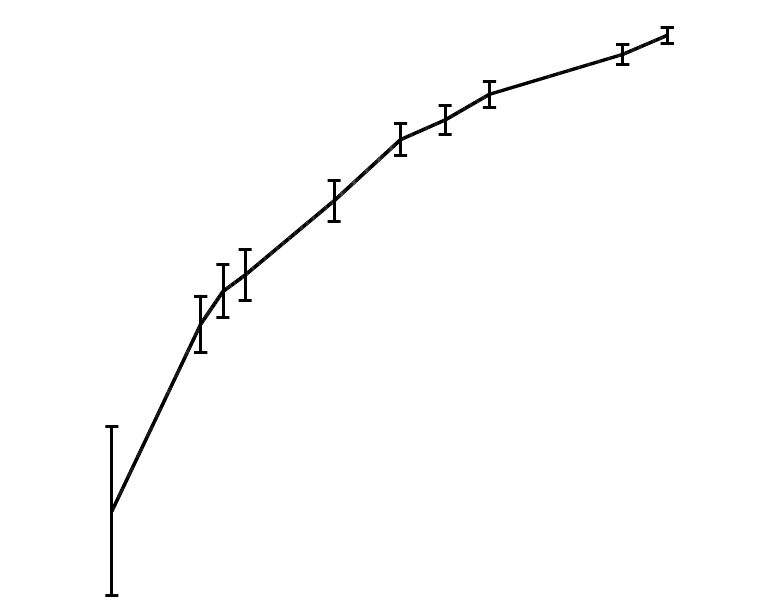
\includegraphics[width=6cm]{img/chap1/reibman1}};
\draw (-7,0) rectangle (0,5.51);
\draw (-7,0.1) -- (-7,0) node[anchor=north] {1};
\draw (-6,0.1) -- (-6,0) node[anchor=north] {1,5};
\draw (-5,0.1) -- (-5,0) node[anchor=north] {2};
\draw (-4,0.1) -- (-4,0) node[anchor=north] {2,5};
\draw (-3,0.1) -- (-3,0) node[anchor=north] {3};
\draw (-2,0.1) -- (-2,0) node[anchor=north] {3,5};
\draw (-1,0.1) -- (-1,0) node[anchor=north] {4};
\draw (0,0.1) -- (0,0) node[anchor=north] {4,5};
\draw (-6.9,1.83) -- (-7,1.83) node[anchor=east] {-5};
\draw (-6.9,3.67) -- (-7,3.67) node[anchor=east] {0};
\draw (-6.9,5.51) -- (-7,5.51) node[anchor=east] {5};
\node[below=0.3cm] at (-3.5,0) {Facteur de l'algorithme};
\node[rotate=90] at (-7.7,2.5) {Qualité subjective relative};
% \end{tikzpicture}\end{tikzpicture}}
	\subfloat[Pour une seule image\label{reibman2}.]{\begin{tikzpicture}[scale=0.853]% \begin{tikzpicture}[scale=0.85]
\node at (-3.5,2.75) {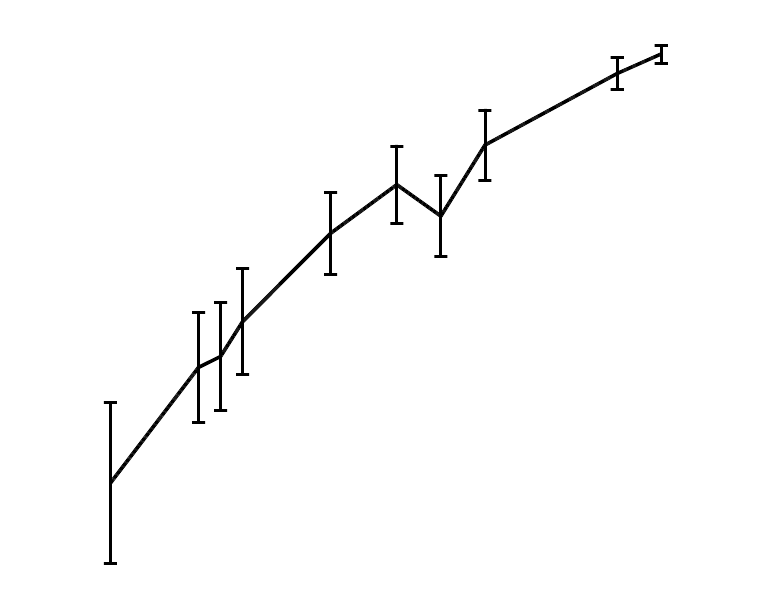
\includegraphics[width=6cm]{img/chap1/reibman2}};
\draw (-7,0) rectangle (0,5.51);
\draw (-7,0.1) -- (-7,0) node[anchor=north] {1};
\draw (-6,0.1) -- (-6,0) node[anchor=north] {1,5};
\draw (-5,0.1) -- (-5,0) node[anchor=north] {2};
\draw (-4,0.1) -- (-4,0) node[anchor=north] {2,5};
\draw (-3,0.1) -- (-3,0) node[anchor=north] {3};
\draw (-2,0.1) -- (-2,0) node[anchor=north] {3,5};
\draw (-1,0.1) -- (-1,0) node[anchor=north] {4};
\draw (0,0.1) -- (0,0) node[anchor=north] {4,5};
\draw (-6.9,0) -- (-7,0) node[anchor=east] {-12};
\draw (-6.9,0.56) -- (-7,0.56) node[anchor=east] {-10};
\draw (-6.9,1.1) -- (-7,1.1) node[anchor=east] {-8};
\draw (-6.9,1.65) -- (-7,1.65) node[anchor=east] {-6};
\draw (-6.9,2.2) -- (-7,2.2) node[anchor=east] {-4};
\draw (-6.9,2.76) -- (-7,2.76) node[anchor=east] {-2};
\draw (-6.9,3.31) -- (-7,3.31) node[anchor=east] {0};
\draw (-6.9,3.87) -- (-7,3.87) node[anchor=east] {2};
\draw (-6.9,4.42) -- (-7,4.42) node[anchor=east] {4};
\draw (-6.9,4.97) -- (-7,4.97) node[anchor=east] {6};
\draw (-6.9,5.51) -- (-7,5.51) node[anchor=east] {8};
\node[below=0.3cm] at (-3.5,0) {Facteur de l'algorithme};
\node[rotate=90] at (-8,2.5) {Qualité subjective relative};
% \end{tikzpicture}\end{tikzpicture}}\\
	\caption{Qualité relative en fonction du paramètre de l'algorithme.}
	\label{fig:reibmanVpqm2006}
\end{figure}

Il existe d'autres modèles de comparaison par paires~\cite{scheffe-jasa,kendall-biometrics,morrissey-josa}. Handley~\cite{handley-pics2001} montre la supériorité du modèle de Bradley--Terry face à la loi du jugement comparatif de Thurstone--Mosteller~\cite{thurstone-psychometrika,mosteller-psychometrika1, mosteller-psychometrika2}, très utilisée par ailleurs~\cite{imberty-rsa,bradlow-jasa}. L'avantage principal du modèle de Bradley--Terry est son efficacité dans le cas où le nombre de comparaisons par paires n'est pas le même pour toutes les images. Cependant, il existe deux importantes restrictions à son usage. La première est que l'ensemble de séquences ne doit pas être décomposables en deux sous-ensembles tels qu'aucune comparaison n'ait été effectuée entre eux. La deuxième est que ces deux sous-ensembles ne doivent pas être tels que toutes les séquences d'un sous-ensemble soient toujours préférées à toutes celles de l'autre sous-ensemble.


\section{Applications en télévision haute définition} \label{tests:TVHD}
Les sections précédentes présentaient des outils en grande partie développés spécifiquement pour la télévision standard. Dans le cadre de leur adaptation à la télévision haute définition, nous devons répondre aux questions suivantes :
\begin{itemize}
\item quelles sont les différences fondamentales entre TVSD et TVHD en termes de conditions de tests ?
\item ces différences ont-elles des conséquences sur les méthodologies déjà existantes et d'autres méthodologies sont-elles à développer ?
\item existe-t-il des expérimentations ayant évalué la qualité visuelle de la TVHD ?
\end{itemize}

Cette section détaille les différences entre TVSD et TVHD qui ont le plus d'influence sur le jugement d'un observateur. Puis nous présenterons trois expérimentations, réalisées par des institutions internationales, sur l'impact de différents facteurs de la TVHD sur la qualité.


\subsection{Que change la télévision haute définition ?} \label{ssec:Que_change_la_télévision_haute_définition}
La télévision haute définition est considérée comme un pas en avant en termes de qualité visuelle. Deux facteurs principaux sont en cause. D'un coté, la plus grande immersion dans l'action est possible grâce au changement de résolution intrinsèque de 720\texttimes576 à 1920\texttimes1080, au passage du format 4$:$3 au format 16$:$9 et plus accessoirement au passage d'un pixel de format 10/9 à un pixel carré. D'un autre côté, l'arrivée à maturité de technologies d'affichage sur écrans plats et de stockage de grande capacité permettent la réalisation technique d'études amorcées au début des années 1980~\cite{fujio-futureHDTV,mitsuhashi-scanning,yuyama-largescreeneffects}. Nous détaillons ici les raisons techniques et psychophysiques du gain en qualité constaté.

\subsubsection{Une qualité accrue par un champ visuel élargi}
Contrairement à la voix et à l'écrit, l'image permet la réception directe d'une grande quantité d'information. À l'époque de sa mise en place, la TVSD devait faire face à des contraintes techniques importantes, notamment au niveau des débits de transmission et des afficheurs. C'est la raison pour laquelle l'image fournie avait un impact visuel réduit sur l'observateur car les technologies ne pouvaient exploiter tout le potentiel des fonctions psychophysiques du système visuel humain. Les sensations et l'émotion ressenties étaient pauvres.

Pour atteindre un plus grand impact psychologique, comme peut le faire le cinéma par exemple, il faut faire converger la zone d'image avec le champ visuel de l'observateur. Cela permet de réduire la sensation de présence de l'appareil de restitution, et de donner de la profondeur et du naturel à l'image. Un tel effet psychologique apparait pour un angle visuel de 20 à 30 degrés dans la direction horizontale. Parallèlement, deux impératifs sont à respecter. Tout d'abord, la structure en lignes ne doit pas être visible. La continuité spatiale de l'image doit donc être assurée. Dans cette optique, la valeur retenue dans le cadre de la TVSD est un ratio entre distance d'observation et hauteur de l'écran égal à six. Dans le cadre de la TVHD, ce ratio est à recalculer. Le second impératif est que le mouvement doit rester fluide, tout en considérant que le système visuel humain ne peut pas suivre un mouvement trop rapide. Le tableau~\ref{tab:DistanceLigneAngle} donne le nombre minimal de lignes que doit contenir une image pour obtenir l'angle visuel donné dans la direction horizontale, en se situant à la distance $O$ de l'écran, le tout sans pouvoir différencier le fait que l'image est constituée de lignes~\cite{fujio-futureHDTV}. La distance $O$ est donnée comme un multiple de la hauteur $H$ de l'écran. Très tôt, des tests ont permis de déterminer la distance idéale pour regarder une image animée sans générer de fatigue~\cite{fujio-futureHDTV,mitsuhashi-scanning,yuyama-largescreeneffects}. Celle-ci est de quatre fois la hauteur de l'écran pour des scènes contenant du mouvement rapide et de trois fois la hauteur de l'écran pour les autres scènes. Ainsi d'après le tableau~\ref{tab:DistanceLigneAngle}, il faut une image d'environ 1200 lignes. C'est un peu plus que le double de celle d'une image de TVSD.

\begin{table}[htbp]
\centering
\begin{tabular}[c]{ccccccc}\toprule
\strong{distance} $O$					& 7,2$H$	& 4$H$		& 3,3$H$	& 3$H$		& 2,5$H$	& 2$H$	\\\midrule
\strong{angle visuel $\Theta$ (degré)}	& 10,7		& 23,5		& 28,3		& 31,0		& 36,9		& 45,2	\\\midrule
\strong{nombre de lignes} $N_L$		& 525		& 940		& 1125		& 1240		& 1480		& 1840	\\\bottomrule
\end{tabular}
\caption{Nombre de lignes $N_L$ requis pour obtenir l'angle visuel $\Theta$ dans la direction horizontale, en se situant à la distance $O$ de l'écran et sans distinguer les lignes.}
\label{tab:DistanceLigneAngle}
\end{table}

Pour augmenter l'impact psychologique de la télévision, la solution consiste donc à agrandir l'image, afin de pouvoir bénéficier d'un angle visuel d'environ 30 degrés en se plaçant à environ trois fois fois la hauteur de l'écran. C'est ainsi que se justifie les dimensions de la télévision haute définition. Plus récemment, d'autres études sont venues confirmer ces valeurs~\cite{svt-assesstudy} et VQEG les utilise dans ses expérimentations~\cite{vqeg-hdtvtestplan}. La proportion de champ visuel excité par l'image passe ainsi de 4\% à 20\% comme l'illustre la figure~\ref{fig:champVisuelHD}. Cependant, une telle augmentation a des conséquences sur l'observateur. Souvent en mouvement, la zone d'intérêt est plus importante, et demande donc une plus grande attention. Les effets de cette immersion sur la perception de l'image nécessitent des études différentes de celles réalisées pour la télévision standard.

\begin{figure}[htbp]
  \centering
  \begin{tikzpicture}[text centered, scale=1.2]\draw[dashed] (0.5,1.5) node[above right] {champ visuel} node[below right] {100\%}-- (0,0) -- (0.5,-1.5);
\filldraw[fill=blue!30] (0,0) node[right=7cm] {20\%} -- (8,2) -- (8,-2) -- cycle;
\filldraw[fill=blue!10] (0,0) node[right=3cm] {4\%} -- (4,0.55) -- (4,-0.55) -- cycle;
\draw (8,2) rectangle node[rotate=90] {TVHD} (8.5,-2);
\filldraw[fill=white] (4,0.55) rectangle node[rotate=90] {TVSD} (4.5,-0.55);
\end{tikzpicture}
  \caption{Proportions de champ visuel excité par les formats TVSD et TVHD.}
  \label{fig:champVisuelHD}
\end{figure}


\subsubsection{Un manque de matériel disponible}
La TVHD manque encore de matériel spécifique tant en production qu'en test ou en visualisation. De même, les protocoles de tests subjectifs sont encore à spécifier, VQEG y consacre d'ailleurs une partie de ses activités~\cite{vqeg-hdtvtestplan}. Les différences avec la TVSD y sont peu marquées à l'heure actuelle, et elles concernent surtout les spécifications de l'environnement de test. Parallèlement, la réalisation de ces tests pour les laboratoires nécessite de pouvoir disposer de vidéos au format TVHD, si possible libres de droits. Actuellement, quelques séquences sont disponibles mais le format est encore minoritairement utilisé. Certains contenus, comme les évènements sportifs, sont particulièrement difficiles à obtenir, alors que leur intérêt est primordial dans l'optique de l'établissement d'un large service de TVHD.

Ce manque rend difficile les études sur télévision haute définition et notamment l'évaluation subjective de la qualité visuelle. Cela explique donc le peu d'études spécifiques à ce format dans la littérature, et particulièrement dans le monde universitaire. Pourtant, l'enjeu scientifique et technique qu'est la mise en place d'un système de TVHD est important.


\subsection{Expériences sur l'impact de la technologie d'affichage} \label{ssec:itu}
En 2005, l'ITU a publié les résultats d'une étude effectuée par l'\emph{Association of radio industries and businesses} japonaise~\cite{itu-crtlcd}. Le but était de comparer les écrans de type CRT aux écrans de type LCD. La méthodologie d'évaluation utilisée était une méthodologie de comparaison simultanée avec une échelle à sept niveaux. Ici, seuls des experts ont pris part aux tests mis en place selon la recommandation spécifiquement dédiée à la TVHD, l'ITU-R BT.710-4~\cite{itu-bt710-4}. Les deux écrans testés étaient un CRT d'usage professionnel de 24 pouces et de résolution 1920\texttimes1080 et un LCD grand public de 23 pouces et de résolution 1280\texttimes768. Les séquences étaient au nombre de 30.

Les résultats montrent une légère préférence pour le CRT. Les meilleurs scores de qualité en sa faveur sont obtenus avec des séquences contenant soit du mouvement, soit des zones sombres. Or, le flou de mouvement et le rendu des zones sombres sont deux des défauts connus du LCD. De plus, la différence de résolution était en défaveur du LCD et était clairement perçue par les experts. Par contre, les couleurs sont mieux appréciées sur le LCD, ainsi que le rendu des zones claires.

Bien sûr, cette étude ne permet pas de conclure catégoriquement sur les différences de qualité entre CRT et LCD. Néanmoins, elle souligne la nécessité d'étudier les différences de technologie, à l'heure où le CRT cède sa place aux technologies à écrans plats.


\subsection{Expériences sur l'impact du format d'image dans un contexte de codage \avc} \label{ssec:ebu}
\begin{wrapfigure}{r}{0.3\linewidth}
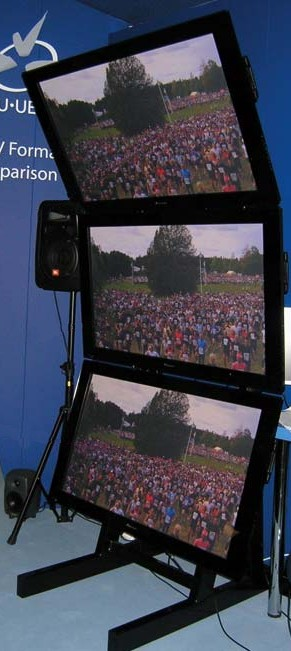
\includegraphics[width=1\linewidth]{img/chap1/ebu}
\caption{Montage de visualisation simultanée de trois écrans HD.} % FIXME voir la mise en page une fois le texte fixé
\label{fig:TroisEcransEBU}
\end{wrapfigure}
Lors de l'\emph{International Broadcasting Convention} de septembre 2006, l'EBU a effectué une expérimentation auprès des participants~\cite{hoffmann-ibc2006}. La démonstration, très formelle étant donné le contexte, permettait de comparer les trois formats de TVHD : 720p/50, 1080i/25 et 1080p/50. Le même contenu était projeté simultanément sur trois écrans 1080p. La figure~\ref{fig:TroisEcransEBU} présente le montage permettant cette visualisation simultanée. Le but était de comparer directement la qualité visuelle de la TVHD en mode entrelacé et en mode progressif, et notamment de montrer l'intérêt du 720p. C'est pourquoi celui-ci était placé sur l'écran du centre. Huit personnes pouvaient s'installer simultanément : quatre à une distance de trois fois la hauteur d'un écran et quatre à quatre fois la hauteur d'un écran. Les séquences utilisées ont été fournies par le SVT et l'EBU et codées par le codeur de référence \avc{} à 20, 18, 16, 13, 10, 8 et 6 Mbps. Les contenus aux formats 1080i et 720p étaient issus du format 1080p en subissant respectivement un désentrelacement et un sous-échantillonnage.

Avec les séquences non compressées, les observateurs percevaient peu de différences entre les trois formats, même à une distance de visualisation de trois fois la hauteur de l'écran. Par contre, suivant la distance d'observation et le contenu, les dégradations apparaissaient avec la compression. Le format 720p donnait une meilleure qualité que le format 1080i pour toutes les séquences et à tous les débits. De plus, plus le débit diminuait, plus les différences entre les formats 720p et 1080i étaient marquées. Enfin, en comparant les formats 720p et 1080p, les observateurs les évaluaient de manière équivalente à haut débit. Par contre, le format 720p était plus apprécié que le format 1080p à bas débit. L'EBU explique cela par le fait que le format 1080p surcharge le codeur en information. Ainsi, suivant le contenu, cette surcharge devient le facteur dominant dans la dégradation de la qualité.

Cette étude, bien que peu formalisée, est intéressante, non seulement pour l'originalité de son installation, mais également pour ses conclusions. Ce n'est pas la première fois que l'EBU affirme la supériorité du format 720p sur le format 1080i et le conseille en production~\cite{wood-hd4u,laven-hdtvWars}. Néanmoins, le marché européen se dirige plutôt vers le 1080i, ce qui risque d'amplifier la problématique de l'évaluation de la qualité. Enfin, si le format 1080p semble montrer de bonnes performances à très haut débit, il nécessite encore des études plus approfondies.


\subsection{Expériences sur l'impact des formats d'image et d'écran dans un contexte de codage MPEG-2} \label{ssec:svt}
Un rapport sur l'évaluation de qualité de séquences HD et SD a été publié en 2002 par la chaine de télévision suédoise SVT~\cite{svt-assesstudy}. Trois études y sont décrites. La première évalue la TVSD sur des écrans de résolution 852\texttimes480. La deuxième s'intéresse aux différences entre la TVSD et la TVHD 720p sur ces mêmes écrans et sur des écrans de résolution 1366\texttimes768 pixels. Enfin, la troisième décrit les différences entre la TVSD et la TVHD 1080i sur des écrans de résolution 1366\texttimes768. Cette dernière étude porte également sur le gain en codage MPEG-2 à l'utilisation du format 720p à la place du format 1080i. Les paramètres utilisés sont le débit, le contenu des séquences et la distance d'observation. Les séquences pour chaque format ont été codées à six débits différents. Pour le format TVHD, les débits utilisés sont : environ 600 megabits par seconde (Mbps) pour la version non compressée, puis 22, 19, 16, 13 et 10 Mbps. Pour le format TVSD, les débits sont : environ 120 Mbps pour la version non compressée, puis 13, 10, 8, 6 et 4 Mbps. Les tests ont été réalisés avec une distance d'observation variant de quatre à six fois la hauteur de l'écran. Les séquences utilisées ont été créées pour ces tests et sont depuis à la disposition de la communauté scientifique. Deux ensembles d'observateurs les ont évalué. Le premier était composé d'experts en qualité vidéo, le second comportait des personnes non expertes. Les écrans utilisés étaient soit de type PDP \emph{(plasma display panel)} de 42 à 50 pouces, soit des CRT de 17 à 32 pouces. Les experts n'ont visualisé qu'une seule des quatre séquences, mais il s'agissait de celle considérée comme la plus critique. La méthodologie d'évaluation retenue a été le DSCQS, présentée en~\ref{tests:dscqs}. L'échelle des adjectifs qualificatifs a dû être traduite en suédois, à partir des versions déjà existantes. Ceci montre que les termes utilisés sont ressentis différemment suivant les cultures et qu'établir une échelle de qualité demande notamment de prendre en compte les spécificités culturelles de la population composant un panel d'observateur. Cela montre également que ce panel doit avoir une certaine cohérence vis-à-vis de la manière dont les tests dont réalisés.

Le premier enseignement de ce rapport est que les résultats des non experts sont confirmés par ceux des experts. C'est pourquoi nous nous contenterons de l'analyse plus critique de ces derniers. La figure~\ref{fig:svtAssessStudy} présente un exemple de résultats obtenus sur deux séquences par les formats TVSD et TVHD 1080i. Les experts considèrent que la TVSD à 4 Mbps sur un écran de 50 pouces de résolution 1366\texttimes768 produit des images de qualité non acceptable. Même sans compression, l'adaptation de l'image à une résolution plus élevée engendre des dégradations trop visibles pour une utilisation courante. Cela suggère donc que la TVSD ne doit pas être utilisée à des résolutions supérieures à celles qu'elle connait déjà. Par contre, le format 1080i est celui attendue pour un écran de 50 pouces. Cependant, dès 22 Mbps, des distorsions deviennent perceptibles. En descendant à un débit de 10 Mbps, le format 720p est bon, même si quelques dégradations sont visibles. La TVSD n'est pas assez bon et le format 1080i est clairement jugé non acceptable à un tel débit en MPEG-2. L'étude voit en cette dernière comparaison la preuve que le mode progressif est meilleur en terme de codage. Ce gain pourrait permettre de transmettre à la fois un flux TVHD et un flux TVSD. Enfin, les observateurs ont considéré comme idéale une distance d'observation de 4 fois la hauteur d'écran.

\begin{figure}[htbp]
	\centering
	\subfloat[Séquence \emph{Knightshields}.]{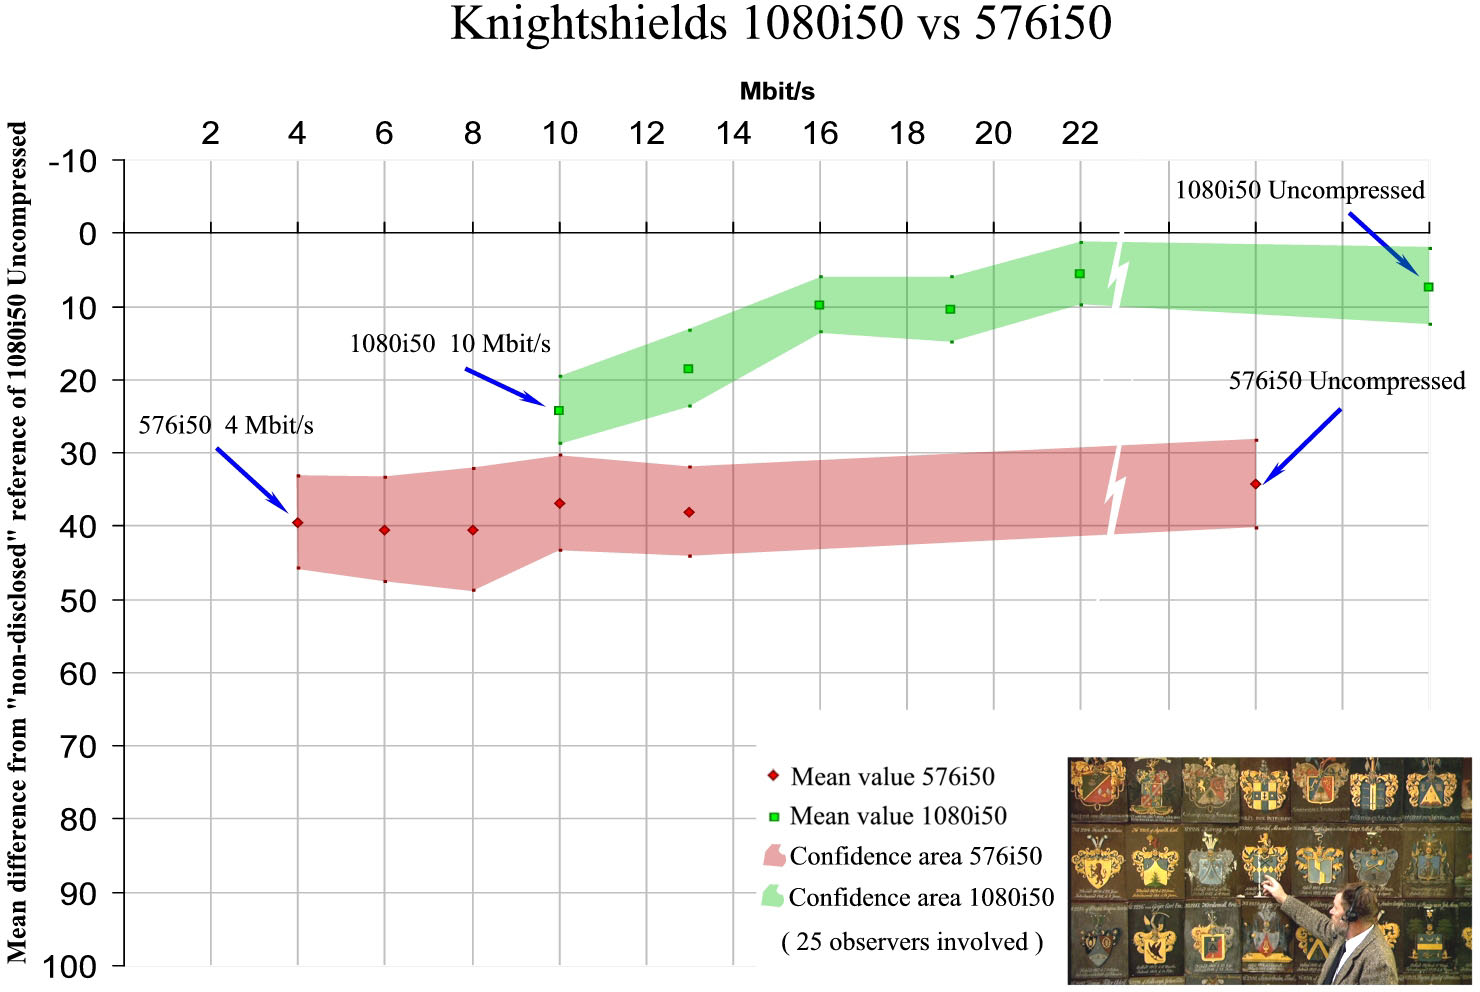
\includegraphics[width=0.48\linewidth]{img/chap1/svt-shields}}\hfill
	\subfloat[Séquence \emph{Stockholm Pan}.]{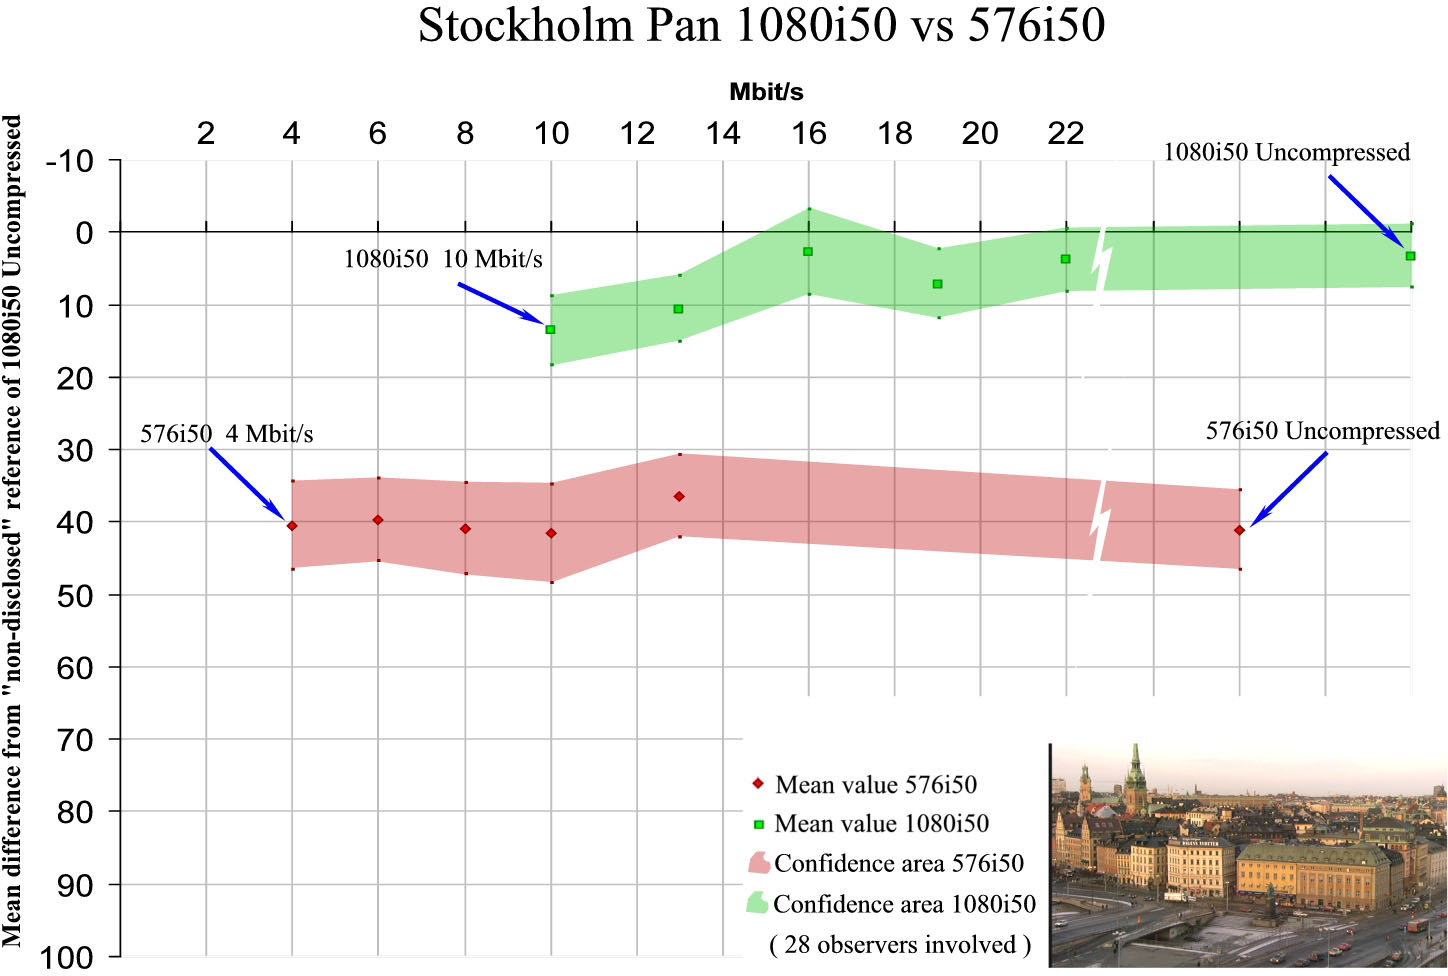
\includegraphics[width=0.48\linewidth]{img/chap1/svt-stockholm}}\\
	\caption{Exemple de résultats obtenus par SVT~\cite{svt-assesstudy}.}
	\label{fig:svtAssessStudy}
\end{figure}

Ce rapport est intéressant pour l'étude de la transition de la TVSD à la TVHD. Elles montrent les lacunes de la TVSD et le gain en qualité des formats 720p et 1080i sur des écrans de haute résolution. Cependant, aucun des écrans utilisés n'offrait les résolutions natives 1280\texttimes720 ou 1920\texttimes1080. De plus, il n'est pas prévu d'utiliser le codage MPEG-2 à terme pour de la diffusion HD. L'évaluation des performances du codage \avc{} est donc importante à réaliser, et ce sur des résolutions qui seront celles utilisées à plus ou moins long terme, à savoir le format 1080i et le format 1080p.


\subsection{Conclusion}
Dans cette section, nous avons explicité les changements induits par la télévision haute définition. Cela a permis de mettre en évidence le fait que ces changements étaient substantiels et que leurs conséquences sur l'évaluation subjective de la qualité devaient être étudiées en profondeur. Nous avons également présenté quelques applications récentes à la télévision haute définition de méthodologies existantes. Toutes ont été réalisées par des institutions, l'implication du monde universitaire dans ce domaine étant particulièrement faible. Ces études proposaient l'analyse d'un des facteurs nouveaux de la TVHD comme la résolution ou le type d'affichage. Malheureusement, la seule étude à utiliser des écrans de résolution 1920\texttimes1080 a réalisé ses tests dans un environnement non normalisé et de manière très informelle, sans relever de données quantitatives. Il y a donc encore de nombreux paramètres à caractériser, en se plaçant dans les conditions réelles du service futur de la TVHD, à savoir avec un écran plat de résolution 1920\texttimes1080 et un système de codage \avc.


\section{Conclusion}
Ce premier chapitre a introduit certains concepts de la problématique d'évaluation subjective de la qualité visuelle en télévision haute définition. Tout d'abord, nous avons présenté les méthodologies les plus couramment utilisées. Nous avons vu qu'il en existe plusieurs, chacune ayant un objectif particulier. Comme certaines études ont pu le montrer, elles ne sont pas interchangeables. Leur principal défaut est qu'elles concernent en grande partie la TVSD, les spécificités de la TVHD n'ayant pas encore été suffisamment considérées dans la normalisation internationale. Ensuite, nous avons présenté la manière dont les évaluations récoltées sont analysées. Cette étape est fondamentale, à la fois pour la vérification de la cohérence des observateurs, mais également pour la synthèse des données en quelques valeurs numériques significatives. Enfin, nous avons détaillé les différences entre la télévision standard et la télévision haute définition. Celles-ci influent sur la manière dont l'évaluation subjective de la qualité doit être pensée pour la TVHD. Des études sur l'impact de la TVHD sur la perception de la qualité ont également été présentées.

Par leur nombre, ces études montrent le peu d'éléments existant sur l'évaluation subjective de la qualité visuelle spécifique à la TVHD. Pire, aucune des expérimentations évoquées ne se place dans des conditions idéales d'évaluation normalisées de la TVHD telle qu'elle est en cours d'apparition en Europe. D'ailleurs, les recommandations internationales, très utilisées pour la TVSD, ne considèrent pas les évolutions majeures induites par cette transition. Celles-ci sont à la fois d'ordre technique et psychophysique. Le côté psychophysique est introduit par la distance d'observation, fortement réduite en TVHD. Cela entraine un plus grand champ visuel excité, et donc une perception de la qualité et des dégradations profondément modifiée. D'un point de vue technique, l'affichage subit une mutation importante puisque les écrans CRT cèdent irrémédiablement la place aux écrans plats, plus grands, moins encombrants et plus lumineux. Ce changement de technologie d'affichage a évidemment des répercussions sur la perception de l'image par l'observateur et peut engendrer tantôt une perte tantôt un gain en qualité qu'il convient d'estimer.


\ornementChapitre

% %%%%%%%%%%%%%%%%%%%%%%%%%%%%%%%%%%%%%%%%%%%%%%%%%
%%%
%%% Auteur : Stéphane Péchard - stephane.pechard@univ-nantes.fr
%%% Fichier : 5-HDvsSd.tex - chapitre 5 : La haute définition et son contexte qualitatif : vers une expérience utilisateur accrue (30 pages)
%%% Version : 0.1
%%% Date : 2007/10/09
%%%
%%%%%%%%%%%%%%%%%%%%%%%%%%%%%%%%%%%%%%%%%%%%%%%%%
\chapter{Contexte qualitatif de la télévision haute définition : évaluation, résolution, affichage} \label{chap:QoEinTVHD}
\opt{final}{\lettrine[lines=4]{N}{ous avons vu au chapitre précédent}}\opt{nofinal}{Nous avons vu au chapitre précédent} que les méthodologies d'évaluation subjective de la qualité visuelle présentent des différences pouvant introduire un biais dans la mesure. Le choix d'une méthodologie a donc son importance et doit répondre à un objectif précis. C'est seulement une fois la méthodologie adéquate déterminée que des tests d'évaluation subjective de la qualité de séquences vidéo peuvent être menés. De tels tests permettent alors d'apporter des réponses aux questions soulevées dans le chapitre précédent.

En premier lieu, nous savons que la télévision haute définition arrive sur un marché où elle doit cohabiter pendant quelques années avec la télévision standard. Le gain en qualité visuelle doit être immédiatement perceptible par les utilisateurs. Cette problématique est particulièrement importante pour les diffuseurs de contenu et les constructeurs de matériel. De plus, ces derniers ne produisent pas d'écran de type CRT pour la TVHD. Les écrans plats de type LCD ou plasma les ont supplantés. Ce changement de technologie a évidemment son importance.

Ce chapitre a pour objectif d'apporter des réponses aux questions concernant la qualité visuelle que nous avons laissées en suspens au chapitre précédent. Nous commencerons par clarifier la problématique, les objectifs et les motivations. Puis, la première question que nous aborderons est liée aux méthodologies d'évaluation subjective de la qualité. Nous cherchons à déterminer si les différences que nous avons évoquées dans la section~\ref{sec:ComparaisonDesMethodes} ont une influence particulière dans un contexte de haute définition. Ceci nous permet également de statuer sur la méthodologie à utiliser pour nos propres évaluations. Nous présenterons ensuite une comparaison directe entre la TVHD et la TVSD. Nous chercherons à savoir comment les différences entre ces deux systèmes influent sur la qualité d'image. Enfin, le remplacement des écrans CRT par des écrans plats de type LCD n'est pas anodin. Il a également son impact sur la perception de la qualité. C'est pourquoi nous nous préoccuperons aussi de cet aspect.


\section{Problématique, objectifs et motivation}
Cette première section situe clairement la problématique qui est la nôtre et les objectifs que nous nous fixons. En effet, le jugement de qualité d'un média comme la télévision est une tâche très complexe. Il nous faut donc réduire le problème. En l'occurrence, nous nous limitons à l'aspect visuel de la qualité. Celui-ci, mieux connu pour la TVSD, subit de profonds changements lors de la transition vers la TVHD. Ces changements sont encore peu connus et c'est pour cela que nous nous y intéressons. Enfin, l'un des points d'intérêt de ce chapitre est l'impact des technologies d'affichage. Nous approfondirons ce point en particulier.


\subsection{Vers la simplification d'une mesure multimodale complexe}
Nous cherchons à mettre en évidence certains aspects de la qualité visuelle en télévision haute définition. Cependant, nous considérons que la qualité visuelle n'est qu'un des aspects de la qualité d'usage. Corrie~\cite{corrie-wace2003} définit cette qualité d'usage comme l'ensemble des caractéristiques de sensation, de perception et d'opinion des êtres humains dans l'interaction avec leur environnement. Ces caractéristiques peuvent aussi bien relever de l'agréable que du désagrément. Il s'agit en tout cas toujours de sensations humaines purement subjectives. Cette définition générale place clairement l'utilisateur comme centre des intérêts, ce qui rend la tâche considérablement complexe. Il est d'ailleurs impossible d'y parvenir sans plusieurs simplifications.

Dans notre contexte, la qualité d'usage résulte de l'interaction d'un utilisateur avec le système de télévision considéré. Ce système doit être capable d'apporter satisfaction à son utilisateur. Bien sûr, nous ne nous intéressons pas à la qualité culturelle du contenu. De plus, aucune interaction avec d'autres personnes n'est considérée. Enfin, le système que nous considérons est unimodal, dans la mesure où seule la qualité visuelle de l'image est considérée par souci de simplification. Les évaluations du son, de l'ergonomie ou encore de l'interaction ne sont pas intégrées à notre étude. Ainsi, les mesures de qualité exploitées sont des MOS issus d'évaluations subjectives de la qualité visuelle, relatifs à un type de média, obtenus dans un environnement contrôlé et sans attente particulière de la part de l'utilisateur. Il n'existe d'ailleurs aucune définition d'un MOS multimodal qui prendrait en compte tous les aspects de cette problématique.

Le concept d'observateur moyen entraine l'utilisation de conditions artificielles mais qui assurent la répétabilité d'une session de test. Le modèle recherché résulte de l'avis moyen d'un panel représentatif mais réduit d'utilisateurs potentiels. Chaque observateur est placé dans des conditions de visualisation qui ne sont pas strictement celles qu'il peut connaitre usuellement, mais cela n'a pas d'impact direct sur le jugement qu'il peut délivrer lors d'une évaluation réalisée dans une salle normalisée. Par contre, il est impératif de garder à l'esprit la nature exacte et les conditions d'obtention d'un tel modèle.


\subsection{De profonds changements}
La section~\ref{ssec:Que_change_la_télévision_haute_définition} détaille ce que les changements technologiques de la télévision haute définition engendre sur la perception de la qualité. Ces modifications sont telles que l'usage du service n'est pas comparable avec celui de la TVSD. Illustrons cela par une expérimentation simple. Elle consiste à mesurer la distance d'observation préférée de l'utilisateur moyen devant un écran de TVHD. Il n'est cependant pas averti du fait qu'il s'agisse d'un tel écran. Le critère retenu est le confort de visualisation. Chaque observateur exprime sa préférence en modifiant la position de son siège par rapport à l'écran, tout en restant dans l'axe de celui-ci. Ce test a été réalisé par des personnes différentes, à la fois avec un écran CRT de hauteur d'image 20,5 centimètres et avec un écran LCD de hauteur d'image 46 centimètres. D'après les recommandations internationales~\cite{itu-bt500-11}, les distances d'observation recommandées sont donc respectivement 61,5 et 138 centimètres en TVHD. Une longue séquence vidéo au format 1080i est utilisée. Sans qu'aucune méthode de rejet n'ait été appliquée, 21 personnes ont pris part à ce test sur CRT et 35 sur LCD. %Leur moyenne d'âge était de 25 ans. Il s'agit en majeure partie d'étudiants masculins. Aucun n'est expert en qualité d'image ni habitué à la TVHD mais tous ont évidemment une certaine expérience de la TVSD et du cinéma.

Avec l'écran CRT, la distance d'observation moyenne mesurée est de 161 centimètres, avec un écart-type de 36 centimètres. Cela correspond à une distance d'environ 7,8 fois la hauteur de l'écran. Avec l'écran LCD, la distance d'observation moyenne mesurée est de 241 centimètres, avec un écart-type de 41 centimètres. Cela correspond à une distance d'environ 5,2 fois la hauteur de l'écran. Tous les observateurs se situent donc très loin de l'écran par rapport aux distances recommandées. Pour le CRT, ils se placent même plus loin que la distance recommandée pour la TVSD. Ils ne profitent donc pas pleinement de l'expérience proposée ni de ce que la TVHD leur permet. Ce résultat est principalement dû à l'habitude culturelle de la TVSD. Les observateurs n'adaptent pas leur comportement de spectateur aux spécificités de la TVHD si ils ne sont pas informés de la possibilité et de l'intérêt psychovisuel de se rapprocher de l'écran. La TVHD est conçue pour être regardée de plus près, mais la qualité visuelle dépend également de la simple connaissance de cette particularité. Dans le cas contraire, la déception pourrait découler de la faible différence ressentie, et se transformer en faible taux d'acceptabilité de service.

% La différence entre les distances d'observation avec le LCD et avec le CRT peut s'expliquer par la différence de taille des écrans. D'une part, un petit écran conduit à une sensation de confinement, proche de celui de la TVSD. La plupart des observateurs font rimer TVHD avec grand écran, donc une taille réduite comme celle du CRT utilisé ne peut, selon eux, pas produire la haute qualité promise. Souvent, l'écran CRT est plus petit que leur propre appareil de télévision. Donc il ne cherche pas particulièrement une meilleure image en s'approchant. D'autre part, l'écran LCD procure une qualité visuelle plus intense. La qualité de la TVHD devient plus évidente. Les observateurs sont plus attirés par le contenu, et sont plus susceptibles de se rapprocher. De plus, la salle de test mesure 5,8 mètres de long et ne permet pas de s'éloigner considérablement. Une minorité d'observateurs se dit être toujours trop près, même située contre le mur. D'où une plus petite distance d'observation moyenne relativement à la hauteur d'écran pour l'écran LCD.

Il est intéressant de noter qu'une fois invités à se placer à la distance normalisée de trois fois la hauteur de l'écran, la plupart des observateurs expriment la sensation d'une image trop grande. La quantité d'information devient difficile à traiter. Ainsi, ils ont besoin de prendre du recul pour la considérer. De plus, pour beaucoup l'écran était tellement proche que le mouvement présent dans les zones périphériques de l'image s'avérait gênant. Ceci s'explique par l'élargissement du champ visuel excité par la TVHD, auquel l'utilisateur de TVSD n'est pas habitué. Le champ visuel horizontal passe d'environ 13° pour la TVSD à environ 33° pour la TVHD, c'est-à-dire de 4\% à 20\% du champ visuel moyen. Cette augmentation n'est pas anodine, surtout que le système visuel humain n'est pas homogène dans l'espace et dans le temps. La vision extra-fovéale est très peu utilisée en TVSD alors qu'elle devient non négligeable en TVHD. %C'est l'un des apports majeurs du format.

Cette simple étude montre le chemin à parcourir en termes d'apprentissage dans l'usage de la TVHD. Pourtant, il s'agit avant tout d'un service de télévision. Le consommateur de TVSD en possède déjà une certaine habitude. Cependant, il doit adapter son comportement aux nouveautés techniques et psychologiques proposées. Pour cela, il est intéressant de mesurer les différences qu'elles représentent. Elles sont sensées être importantes et remarquables pour l'observateur, afin de l'immerger dans l'action. C'est pourquoi nous voulons déterminer la préférence de l'observateur moyen entre la TVHD et la TVSD. Cela peut permettre de déterminer l'influence de la taille de l'écran sur la qualité d'usage. D'autre part, l'intérêt d'une telle comparaison est évident pour les diffuseurs de programmes. En effet, il est difficile de définir précisément le débit à allouer pour atteindre une certaine qualité en fin de chaine. Le cout de la bande passante étant élevé, sa valeur doit être précisément définie. Il est donc nécessaire de déterminer la différence de qualité entre la TVHD et la TVSD et le niveau à atteindre pour s'assurer que l'observateur préfère la TVHD.


\subsection{De l'impact des nouvelles technologies d'affichage}
Il va falloir quelques années de cohabitation de la TVHD et la TVSD avant de voir cette dernière progressivement abandonnée par les diffuseurs. C'est pourquoi les nouveaux téléviseurs sont capables d'afficher les deux technologies. Cependant, la visualisation d'une image 720\texttimes576 sur une dalle de 1920\texttimes1080 points nécessitent une adaptation évidente. La solution la plus simple consiste à la laisser dans sa taille d'origine et à l'entourer de noir. Elle a cependant le désavantage de révéler l'inutilité de disposer d'un si grand écran. La seconde technique consiste à étirer l'image aux dimensions de la dalle d'affichage, parfois sans même conserver l'aspect 4$:$3. Cette technique est le plus souvent privilégiée.

Le dernier aspect de la qualité visuelle en TVHD évoqué dans ce chapitre concerne donc l'affichage d'images de TVHD. Tout d'abord, dans le cadre de la comparaison TVHD et TVSD, nous mesurerons l'impact d'un algorithme de redimensionnement sur la qualité visuelle. Cette étude s'inscrit pleinement dans le marché actuel de la TVHD en Europe. De même, la comparaison des types d'affichage a un intérêt technologique. Nous étudions donc la différence de qualité induite par la différence de technologie d'affichage entre écran CRT et écran LCD.


\subsection{Conclusion}
Dans cette première section, nous avons détaillé les diverses problématiques qui occupent ce chapitre. Cela nous a permis de définir la notion de qualité d'usage, qui est la qualité globale d'un service de télévision. Devant la complexité d'un tel concept, nous le réduisons à la qualité visuelle, mesurée par des tests psychovisuels. Nous avons également introduit les différentes études que menons. En premier lieu, la question de la méthodologie d'évaluation de la qualité visuelle se pose en termes de sens et de pertinence des résultats. Notre première étude consiste donc en la détermination de l'impact de la méthodologie d'évaluation sur les MOS obtenus. %Ensuite, nous effectuons une comparaison entre TVSD et TVHD en termes de qualité d'usage. L'interaction des effets de la taille de l'écran d'un côté et des distorsions de l'autre est analysée. Enfin, la dernière étude porte sur l'influence du type de technologie d'affichage utilisée. Pour cela, nous comparons les qualités mesurées sur un écran de type CRT et un écran de type LCD et nous mesurons l'impact de l'adaptation de l'image à une définition supérieure.


\section{Impact de la méthodologie d'évaluation subjective de la qualité} \label{sec:impactMéthodÉvalSubj}
Tous les MOS que nous exploitons sont issus de tests subjectifs. La méthodologie utilisée pour les obtenir a une importance non négligeable dans le sens du résultat. En effet, la précision d'une mesure de type MOS est entre autre liée au nombre d'observateurs impliqués et au temps passé par chacun ; elle est donc directement liée à la méthodologie d'évaluation. Plusieurs méthodologies d'évaluation subjective de la qualité ont été présentées dans la section~\ref{sec:A_chaque_methodologie_sa_grandeur_mesuree}. Chacune a des caractéristiques distinctes et un cadre d'exploitation restreint. Nous cherchons à évaluer la qualité visuelle ressentie par les observateurs, c'est pourquoi nous utilisons une méthodologie avec une échelle de qualité.

La méthodologie ACR est intéressante par sa capacité à produire une grande quantité de résultats en une session. C'est la principale raison de son succès. D'un autre côté, la méthodologie SAMVIQ est plus longue mais semble plus précise grâce à la possibilité de visualiser plusieurs fois un même stimuli. C'est pourquoi nous comparons ici ces deux méthodologies, détaillées sections~\ref{tests:acr} et~\ref{tests:samviq}. %Les différences entre les méthodes identifiées dans la section~\ref{sec:ComparaisonDesMethodes} sont dans ce cas toutes en vigueur.

Deux éléments sont ici à l'étude. Tout d'abord, nous nous intéressons aux différences entre les résultats fournis par les deux méthodologies. Pour cela, elles sont toutes les deux utilisées pour évaluer un même ensemble de séquences. Puis, l'influence du nombre d'observateurs sur la précision obtenue sera évaluée.


\subsection{Comparaison des évaluations subjectives}
Nous avons utilisé les méthodologies ACR et SAMVIQ pour évaluer un même ensemble de 192 séquences vidéos originales ou dégradées. Les 24 séquences originales et les 168 versions dégradées sont détaillées à l'annexe~\ref{annex:base}. Les mêmes conditions de test sont réunies, elles suivent les recommandations \ituCC{} et ITU-R BT.710-4~\cite{itu-bt710-4}. Les tests utilisant ACR ont nécessité 56 séances de tests sur 6 jours. Ceux utilisant SAMVIQ se sont étalés sur 127 séances de tests et 14 jours.

Étant donné la différence d'échelle entre les deux méthodologies, nous devons adapter les appréciations à une même échelle de notation. Nous pourrons ensuite regarder la relation entre les deux ensembles de données. Enfin, nous comparerons ces résultats avec des données issues d'autres tests, effectués à des résolutions différentes.


\subsubsection{Ajustement des échelles des deux méthodologies}
Les mesures subjectives de qualité données par la méthodologie ACR sont comprises entre 1 et 5, alors que celles de la méthodologie SAMVIQ sont entre 0 et 100. Afin de pouvoir les comparer, une transformation de notes est nécessaire. Sur l'échelle SAMVIQ, les termes sémantiques sont placés au centre des intervalles. La correspondance entre les deux échelles est illustrée par la figure~\ref{fig:diffEchelleACR-SAMVIQ}. Le 1 et le 5 de l'échelle discrète de l'ACR correspondent respectivement au 10 et au 90 de l'échelle continue de SAMVIQ. L'ACR a donc une échelle plus réduite que SAMVIQ, elle ne couvre que 80\% de la gamme SAMVIQ. Formellement, les appréciations données par ACR sont une quantification de celles données par SAMVIQ.

\begin{figure}[htbp]
  \centering
  % schéma de la correspondance entre les échelles des méthodes ACR et SAMVIQ

\begin{tikzpicture}
	% samviq
	\draw (-1,3) node[legende, text width=8em, minimum height = 19em] {};
	\draw (-1,6) node {\textbf{SAMVIQ}};
	\draw (0,0) -- (0,5)
		node at (-1.5,4.5) {excellent}
		node at (-1.5,3.5) {bon}
		node at (-1.5,2.5) {assez bon}
		node at (-1.5,1.5) {médiocre}
		node at (-1.5,0.5) {mauvais};

	\draw (0.1,5) -- (-0.1,5) node[left]{100};
	\draw (0.1,4) -- (-0.1,4);
	\draw (0.1,3) -- (-0.1,3);
	\draw (0.1,2) -- (-0.1,2);
	\draw (0.1,1) -- (-0.1,1);
	\draw (0.1,0) -- (-0.1,0) node[left]{0};


	% acr
	\draw (3,3) node[legende, text width=6em, minimum height = 19em] {};
	\draw (3,6) node {\textbf{ACR}};
	\draw
		node at (1.2,4.5) {5}
		node at (1.2,3.5) {4}
		node at (1.2,2.5) {3}
		node at (1.2,1.5) {2}
		node at (1.2,0.5) {1}
		node[action] at (3,4.5) {excellent}
		node[action] at (3,3.5) {bon}
		node[action] at (3,2.5) {assez bon}
		node[action] at (3,1.5) {médiocre}
		node[action] at (3,0.5) {mauvais};


	% liaison
	\draw[dashed] (0.2,4.5) -- (1,4.5);
	\draw[dashed] (0.2,3.5) -- (1,3.5);
	\draw[dashed] (0.2,2.5) -- (1,2.5);
	\draw[dashed] (0.2,1.5) -- (1,1.5);
	\draw[dashed] (0.2,0.5) -- (1,0.5);

	\draw (0.1,4.5) node[font=\tiny, left]{90};
	\draw (0.1,3.5) node[font=\tiny, left]{70};
	\draw (0.1,2.5) node[font=\tiny, left]{50};
	\draw (0.1,1.5) node[font=\tiny, left]{30};
	\draw (0.1,0.5) node[font=\tiny, left]{10};

\end{tikzpicture}
  \caption{Schéma de la correspondance entre les échelles des méthodologies ACR et SAMVIQ.}
  \label{fig:diffEchelleACR-SAMVIQ}
\end{figure}

Pour réaliser la transformation, les notes issues de ACR sont projetées linéairement sur l'échelle utilisée dans SAMVIQ. La note transformée $\text{MS}'$ est obtenue à partie de la note originale $\text{MS}$ par la formule :
\begin{equation}
\text{MS}' = \left(\text{MS} - 1\right)\times \text{20} + \text{10}.
\end{equation}


\subsubsection{Mise en compétition des évaluations issues des deux méthodologies}
La figure~\ref{fig:nuageACR-SAMVIQ} présente les MOS issus de la méthodologie ACR en fonction des MOS issus de la méthodologie SAMVIQ. Le coefficient de corrélation entre les deux populations de notes est de 0,8993. La racine carrée de l'erreur quadratique moyenne est de 14,06. La corrélation est plus faible que ce nous aurions pu penser a priori, significativement plus que celles obtenues dans des études effectuées à d'autres résolutions~\cite{huynhthu-sip2005, brotherton-ieice2006}. Par contre, la racine carrée de l'erreur quadratique moyenne est forte, très supérieure aux intervalles de confiance à 95\% dont les moyennes sur les 192 séquences sont respectivement de 5,73 et de 6,91 pour les méthodologies ACR et SAMVIQ. Les deux méthodologies produisent donc deux ensembles de MOS qui n'ont pas de relation très forte. Nous ne pouvons pas trouver de modèle fiable qui permettent de transformer les MOS de l'une en MOS de l'autre. Ainsi, bien que leurs buts soient identiques, les deux méthodologies ne fournissent pas des résultats bien superposables entre eux.

\begin{figure}[htbp]
	\centering
	\begin{tikzpicture}[only marks, scale=0.07]
		\pgfsetplotmarksize{1.5cm}
		\draw plot[mark=+] file {plot/chap2/ACR-SAMVIQ.txt};
		\draw plot[mark=o] file {plot/chap2/ACR-SAMVIQ-REF.txt};
		\draw[->] (0,0) -- node[below=0.5cm] {MOS issus de SAMVIQ} (95,0);
		\draw[->] (0,0) -- node[above=0.7cm, sloped] {MOS issus d'ACR} (0,95) ;
		\foreach \x in {0,15,30,45,60,75,90} \draw (\x,1) -- (\x,-1) node[anchor=north] {\x};
		\foreach \y in {0,15,30,45,60,75,90} \draw (1,\y) -- (-1,\y) node[anchor=east] {\y};
		\draw[dotted] (0,0) -- (90,90);
		\draw[legende] (35,5) rectangle (90,20);
		\draw plot[mark=+] coordinates{(40,16)} node[right=5] {versions dégradées};
		\draw plot[mark=o] coordinates{(40,9)} node[right=5] {références explicites};
	\end{tikzpicture}
	\caption{MOS issus de la méthodologie ACR en fonction des MOS issus de la méthodologie SAMVIQ.}
	\label{fig:nuageACR-SAMVIQ}
\end{figure}

La figure montre que les notes ACR se situent, après transformation, à une valeur supérieure à celles produites par SAMVIQ, sauf sur les extrémités. La méthodologie ACR est donc moins critique que SAMVIQ, grâce à laquelle les dégradations sont mieux perçues. Par contre, la figure montre le phénomène inverse pour les notations des contenus de référence, qui sont globalement supérieures quand elles sont produites par SAMVIQ. Pour cette dernière, c'est le MOS de la référence cachée qui est considéré. Quelles différences entre les méthodologies peuvent expliquer le phénomène observé ?

Premièrement, la différence initiale d'échelle implique que les notes produites par la méthodologie ACR, après transformation linéaire, sont limitées à l'intervalle [10 ; 90]. Corriveau a montré que la gamme des notes utilisées dans une échelle discrète est plus grande que celle d'une échelle quasi continue~\cite{corriveau-subjScales}. Nos résultats confirment cette tendance. Avec des valeurs observées minimale de 10 et maximale de 87,04, l'ACR utilise 96,3\% de sa gamme utile, contre 82\% pour SAMVIQ avec un minimum de 6,27 et un maximum de 88,33. Pourtant, les MOS des vidéos de référence issus de l'ACR sont, en moyenne, éloignés de la borne supérieure. Ils sont compris entre 68,52 et 87,04, avec une moyenne de 77,44. Avec une tendance à pleinement utiliser l'échelle, cela n'explique pas complètement le phénomène observé.

SAMVIQ permettant un nombre illimité de visualisation, l'observateur peut les utiliser afin de détecter toutes les dégradations. Il a ainsi tendance à diminuer sa note sur des séquences dégradées. Par contre, pour une séquence de référence, plusieurs visualisations ne le font pas détecter plus de dégradations.

Il est plus difficile de statuer sur l'effet de la présence de la référence explicite. Dans SAMVIQ, l'observateur ne peut pas voir objectivement de différence entre les deux références qu'il visualise. Cependant, dans un contexte de dégradation, la logique voudrait qu'il n'attribue pas de note supérieure à celle qu'il a donné à la référence explicite, même pour la référence cachée. En les comparant, il peut tout au mieux les évaluer identiquement. De plus, l'observateur n'est pas dans les mêmes conditions psychologiques lors de la visualisation des deux références. La référence explicite est clairement identifiée et est évaluée de manière absolue. Par contre, la référence cachée est jugée en comparaison de la référence explicite et ne bénéficie pas du même a priori qualitatif. % Dans ACR, la référence visualisée n'est pas explicite. Bien qu'elle soit située en haut de l'échelle de qualité, elle ne permet pas un ancrage sémantique aussi important.


\subsubsection{Mise en évidence d'une influence de la taille de l'image}
Nous cherchons ici à savoir si la taille de l'image a une influence sur la différence entre le protocole ACR et le protocole SAMVIQ. En effet, alors que Brotherton~\cite{brotherton-ieice2006} obtient un coefficient de corrélation de 0,94 avec des séquences au format CIF (taille 352\texttimes288), nous n'obtenons que 0,8991 pour un format TVHD (taille 1920\texttimes1080). Pour conforter cette tendance, regardons les mêmes données à d'autres résolutions.

Dans le cadre du projet Sc@limages\footnote{De juillet 2006 à juin 2008, le projet Sc@limages a eu pour but de prouver l'intérêt de la technologie de compression graduable dans le cadre du pôle de compétitivité Images et réseaux.}, l'équipe IVC du laboratoire IRCCyN a effectué des tests subjectifs de qualité avec les méthodologies SAMVIQ et ACR. Deux jeux de 28 séquences aux formats QVGA et VGA ont été évalués. Les coefficients de corrélation entre les MOS issus des deux méthodologies sont de 0,969 pour les séquences QVGA et de 0,942 pour les séquences VGA. Le tableau~\ref{tab:resolutionCC} récapitule les résultats obtenus aux différentes résolutions, ainsi que les distances d'observations et les champs visuels correspondants.

\begin{table}[htbp] % formule ((atan((1920/2)/(1080*3))*180)/pi)*2
\centering
\begin{tabular}{ccccc}\toprule
\multirow{2}{2.5cm}{\strong{format}} & \multirow{2}{2.5cm}{\strong{résolution}} & \strong{distance} & \strong{champ} & \strong{coefficient}\\
 & & \strong{d'observation} &  \strong{visuel} & \strong{de corrélation}\\ \toprule
QVGA					& 320\texttimes240			&	6$H$				&	13°		& 0,969			\\ \midrule % 28 points
CIF						& 352\texttimes288			&	6$H$				&	12°		& 0,94				\\ \midrule % ? points
VGA						& 640\texttimes480			&	4$H$				&	19°		& 0,942			\\ \midrule % 28 points
% QHD						& 960\texttimes540			&	6$H$				&	17°		& ?? 					\\ \midrule % 28 points
TVHD					& 1920\texttimes1080		&	3$H$				&	33°		& 0,899			\\ \bottomrule % 192 points
\end{tabular}
\caption{Coefficients de corrélation entre MOS issus des méthodologies ACR et SAMVIQ pour plusieurs résolutions d'image.}
\label{tab:resolutionCC}
\end{table}

Plus l'image est grande, plus le coefficient de corrélation chute. Ainsi, la taille de l'image aurait une réelle influence sur la corrélation entre les MOS issus de l'ACR et SAMVIQ. Ici, ni le type d'échelle ni la présence de la référence explicite n'ont d'influence. Par contre, le nombre de visualisation peut avoir la même influence que lorsque les évaluations des références explicites étaient supérieures pour SAMVIQ. En effet, avec une seule ou plusieurs visualisation, une séquence de taille réduite sera évaluée de la même manière. La revoir à nouveau n'apporte pas d'information sensible sur le jugement qualitatif qu'en fait l'observateur. Par contre, une grande image gagne à être revue. La première visualisation n'est pas suffisante pour l'explorer complètement et évaluer toutes les dégradations. Avec SAMVIQ, la vision multiple d'une séquence permet alors d'affiner le jugement. Ainsi, le choix entre ACR et SAMVIQ pourrait être guidé par la taille des images à évaluer.


\subsubsection{Conclusion}
Nous venons de mettre en évidence des différences entre les MOS produits par les méthodologies ACR et SAMVIQ. Tout d'abord, dans le contexte de la TVHD, nous avons constaté qu'il y a peu de corrélation entre les deux populations de MOS. En effet, le coefficient de corrélation est de 0,8993. Ce résultat est important, car cela signifie que les méthodologies ne sont pas interchangeables et que le choix entre l'une des deux aura une influence sur les MOS obtenus.

De plus, nous avons montré que la taille de l'image évaluée, et donc celle du champ visuel correspondant, avait une influence sur cette différence d'évaluation. Alors qu'avec une image de faible taille, les méthodologies fournissent des résultats très corrélés, ce n'est plus tout à fait le cas avec la TVHD. Nous pouvons donc considérer que les méthodologies ACR et SAMVIQ sont équivalentes jusqu'à une certaine taille de champ visuel. Au-delà, les deux ont des comportements moins similaires. La taille des images testées est donc à prendre en compte dans le choix d'une méthodologie.


\subsection{Influence du nombre d'observateurs sur l'intervalle de confiance à 95\%}
Afin de discriminer de très petites différences de qualité, nous devons utiliser une méthodologie particulièrement précise. Cependant, suivant la méthodologie utilisée, une précision donnée n'est pas fournie par le même nombre d'observateurs. Les méthodologies d'évaluation de la qualité visuelle n'ont donc pas toutes la même précision. Nous mesurons cette précision par l'intervalle de confiance à 95\% calculés sur chaque MOS. Or, le nombre d'observateurs influe non seulement sur la précision, mais également sur la longueur du test. Nous devons donc déterminer l'équilibre précision-nombre d'observateurs adéquat.


\subsubsection{Méthode d'analyse}
Nous cherchons à analyser l'influence du nombre d'observateurs sur l'intervalle de confiance à 95\%. Nous réalisons cela pour les méthodologies ACR et SAMVIQ avec les 192 séquences de la base présentée dans l'annexe~\ref{annex:base}. La première méthodologie est utilisée par $N_\mathit{ACR}$ = 28 personnes. Par contre, étant donné le nombre important de séquences à évaluer, la méthodologie SAMVIQ est effectuée en trois sessions de quatre contenus. Donc, non seulement les observateurs ne sont pas les mêmes d'une session à l'autre, mais leur nombre peut également varier. Les nombres d'observateurs retenus sont ainsi de 22, 21, 22, 16, 15 et 19 pour les sessions SVT2002, Euro1080-1, Euro1080-2, SVT2006-1, SVT2006-2 et SVT2006-3 respectivement.

Les critères de rejet ne sont pas identiques pour chaque méthodologie, ils sont définis par les recommandations de chaque méthodologie. La méthodologie ACR utilise le critère de l'ITU, alors que la méthodologie SAMVIQ utilise son propre critère. Les deux sont présentés au paragraphe~\ref{sssec:rejet-samviq}. Nous calculons donc nos intervalles de confiance dans trois configurations différentes, en utilisant les trois modes de rejet :
\begin{enumerate}
\item sans critère de rejet ;
\item avec le critère de rejet de la méthodologie ACR ;
\item avec le critère de rejet de la méthodologie SAMVIQ.
\end{enumerate}
%
Le tableau~\ref{tab:nbObsRejet} présente le nombre d'observateurs retenus par chaque critère de rejet pour les deux méthodologies. Dans le cas de SAMVIQ, le premier nombre indique le nombre maximal d'observateurs pour lequel toutes les séquences sont disponibles. Le second nombre indique le nombre maximal d'observateurs pour lequel des séquences sont disponibles.

\begin{table}[htbp]
\centering
\begin{tabular}{cccc}\toprule
\strong{méthodologie}	& \strong{sans rejet}	& \strong{rejet ACR}	& \strong{rejet SAMVIQ} \\ \toprule
ACR									& 28								& 27								& 23									\\ \midrule
SAMVIQ								& 18-25						& 15-25						& 15-22							\\ \bottomrule
\end{tabular}
\caption{Nombre d'observateurs retenus par chaque critère de rejet pour les deux méthodologies.}
\label{tab:nbObsRejet}
\end{table}

L'analyse consiste à calculer ces intervalles pour plusieurs nombres $N^P$ d'observateurs. Par exemple, les intervalles de confiance de la méthodologie ACR sont calculés pour $N_{\mathit{ACR}}^P \in$ \{28, 25, 22, 20, 18, 15, 12, 10, 8\}. Pour chaque valeur de $N_{\mathit{ACR}}^P$, les $\text{C}_{N_\mathit{ACR}}^{N_{\mathit{ACR}}^P}$ combinaisons possibles d'observateurs sont calculées et nous appelons intervalle de confiance moyen $\mathit{IC}_{\mathit{ACR}}^{N_{\mathit{ACR}}^P}$ la moyenne de ces intervalles. Par exemple :
\begin{equation}
\mathit{IC}_{\mathit{ACR}}^8 = \frac{1}{\text{C}_{N_\mathit{ACR}}^8} \sum_{k=1}^{\text{C}_{N_\mathit{ACR}}^8} \mathit{IC}_{\mathit{ACR}}(k).
\end{equation}

Dans le cas de la méthodologie SAMVIQ, certaines moyennes sont calculées sur une faible quantité de contenus. En effet, étant donné que le nombre d'observateurs varie d'une session à l'autre, nous ne disposons pas des 192 évaluations pour tous les nombres d'observateurs $N_{\mathit{SAMVIQ}}^P$. Ceci a pour conséquence d'accroitre la dépendance au contenu. Nous ne considérons donc que les moyennes pour lesquelles nous disposons d'au moins 64 valeurs.


\subsubsection{Intervalle de confiance moyen en fonction du nombre d'observateurs}
La figure~\ref{fig:ic-acr} présente l'intervalle de confiance moyen en fonction des différents nombres d'observateurs pour la méthodologie ACR et les trois modes de rejet. La figure~\ref{fig:ic-samviq} est l'équivalent pour la méthodologie SAMVIQ. Comme nous nous y attendions, l'intervalle de confiance moyen décroit avec le nombre d'observateurs, ce qui signifie que la précision croit. Les différences entre les trois modes sont globalement très faibles. Ceci signifie que le critère de rejet a un impact faible sur la précision des évaluations. D'autre part, alors que la précision de la méthodologie ACR semble suivre une loi très stable en fonction du nombre d'observateurs, il en va autrement de la méthodologie SAMVIQ. Ceci est notamment remarquable à partir d'un grand nombre d'observateurs. Ceci s'explique par le fait que la moyenne est calculée sur un nombre plus réduit de contenus comme nous l'avons expliqué précédemment.

\begin{figure}[htbp]
\centering
\subfloat[\label{fig:ic-acr}Intervalle de confiance moyen issu de la méthodologie ACR en fonction du nombre d'observateurs.]{\includegraphics[page=2, width=0.48\linewidth, trim= 70 50 90 70]{plot/chap2/IC-SAMVIQ-ACR}}\hfill
\subfloat[\label{fig:ic-samviq}Intervalle de confiance moyen issu de la méthodologie SAMVIQ en fonction du nombre d'observateurs.]{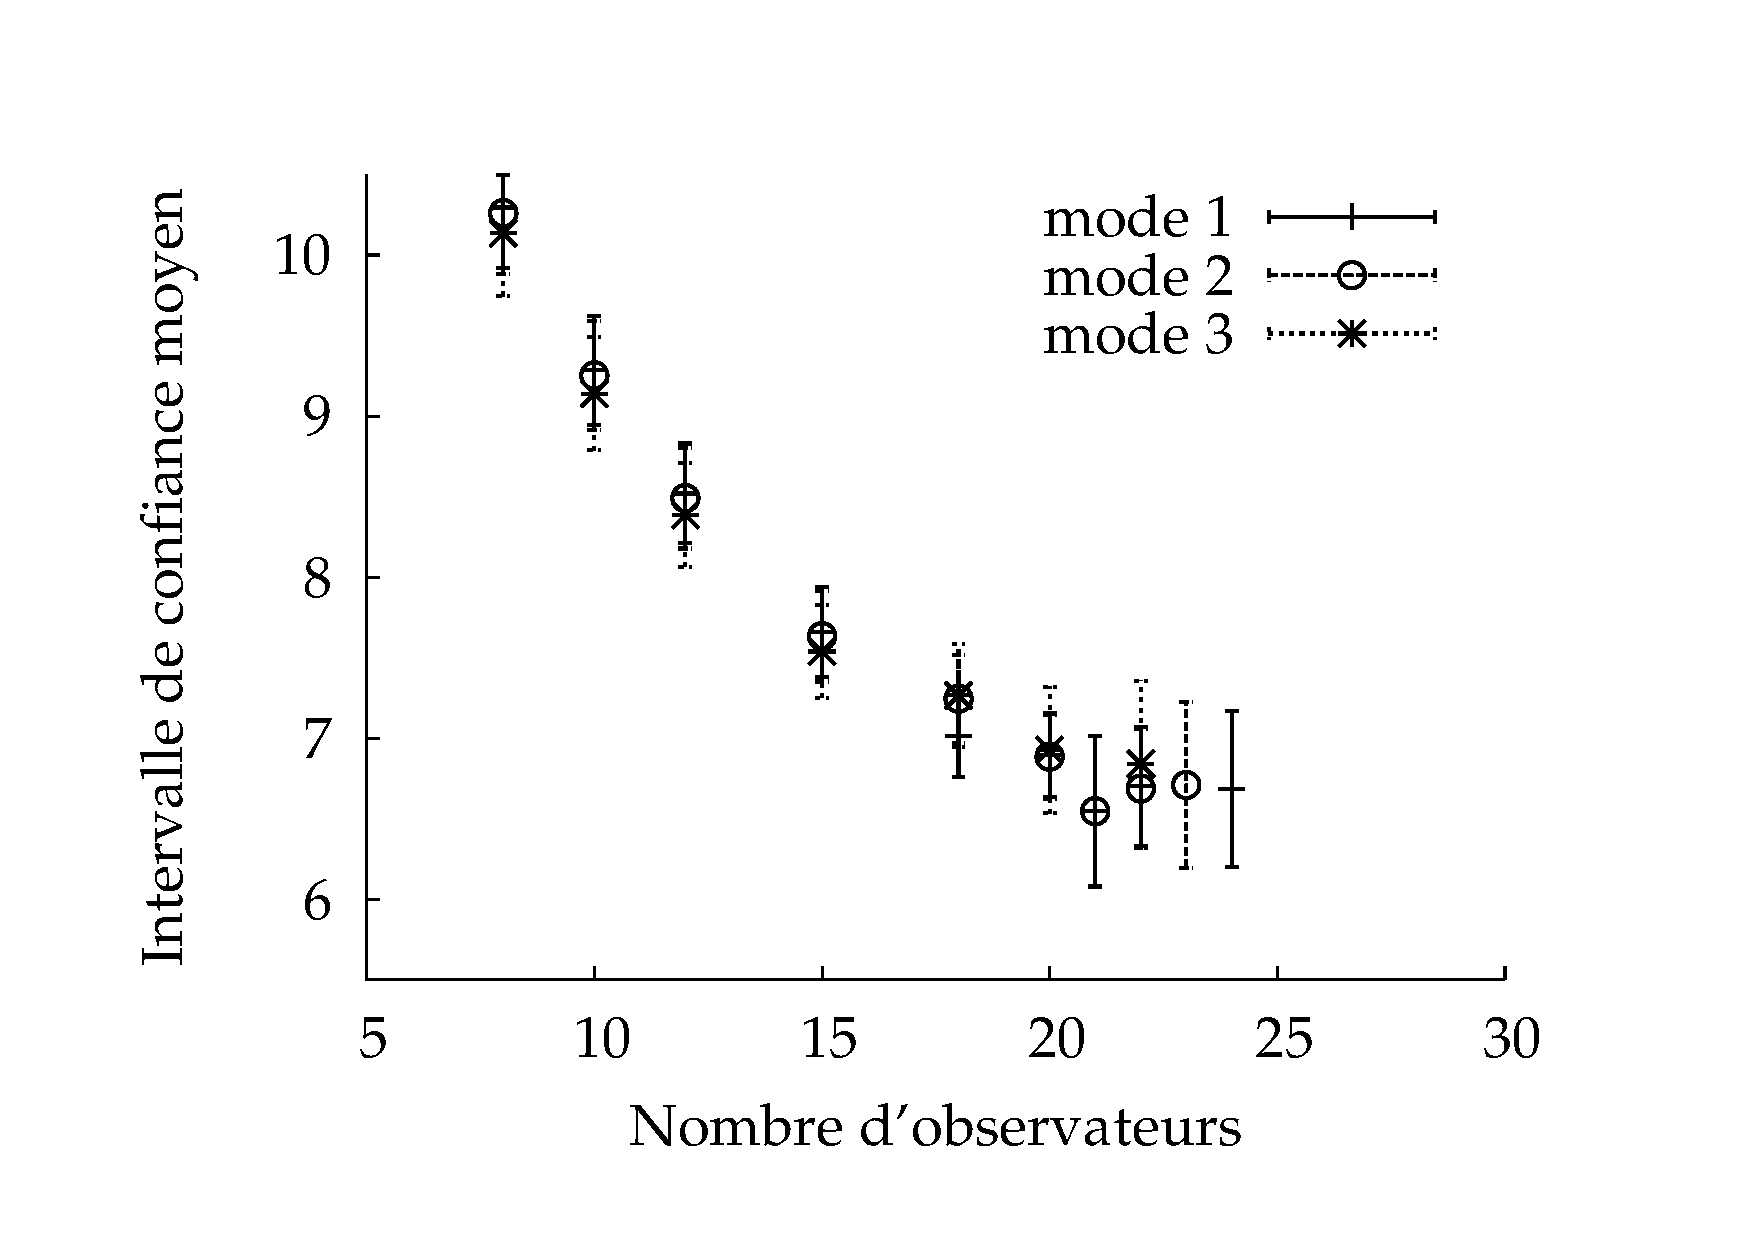
\includegraphics[page=1, width=0.48\linewidth, trim= 70 50 90 70]{plot/chap2/IC-SAMVIQ-ACR}}\\
\caption{Intervalle de confiance moyen en fonction du nombre d'observateurs pour les deux méthodologies et les trois modes de rejet. Les trois modes sont : (1) sans critère de rejet ; (2) avec le critère de rejet de la méthodologie ACR ; (3) avec le critère de rejet de la méthodologie SAMVIQ.}
\end{figure}

Les valeurs obtenues semblent être proches les unes des autres entre les méthodologies ACR et SAMVIQ. Cependant, elles ne tiennent pas compte du fait que la gamme de notation utile est réduite dans la méthodologie ACR. Elle représente seulement 80\% de l'échelle de la méthodologie SAMVIQ. Ainsi, un intervalle de confiance de 10 sur une échelle allant de 0 à 100 est plus précis que ce même intervalle sur une échelle allant de 0 à 80. Afin de pouvoir comparer nos deux ensembles d'intervalles, nous ajustons ceux issus de la méthodologie ACR en leur appliquant un coefficient multiplicateur de 1,25 afin de compenser la différence de gamme des échelles.

Le tableau~\ref{tab:valIC-acr-samviq} présente les intervalles de confiance moyens issus des méthodologies ACR et SAMVIQ sans rejet, avant et après ajustement et les nombres d'observateurs correspondants. Les intervalles de confiance issus de la méthodologie ACR sont tous supérieurs à ceux issus de la méthodologie SAMVIQ. De plus, sachant que le nombre requis d'observateur pour la méthodologie SAMVIQ est de 15, il en faudrait plus de 22 avec la méthodologie ACR pour obtenir la même précision.

\begin{table}[htbp]
\centering
\begin{tabular}{cccc}\toprule
\multirow{2}{2.5cm}{\strong{nombre d'observateurs}} & \multicolumn{2}{c}{\textbf{avant ajustement}} & \textbf{après ajustement}\\
\cmidrule{2-4}
		& \strong{IC ACR }	& \strong{IC SAMVIQ} 	& \strong{IC ACR}\\ \toprule
8		&	10,252					& 10,296						& 12,815		\\ \midrule
10	&	9,253					&	9,284						&	11,567		\\ \midrule
12	&	8,495					& 8,519						&	10,619		\\ \midrule
15	&	7,640					& 7,658						&	9,550		\\ \midrule
18	&	6,999					& 7,014						&	8,749		\\ \midrule
20	&	6,652					& 6,893						&	8,315		\\ \midrule
% 21	&								& 6,545						&	\\
22	&	6,352					& 6,701						&	7,940		\\ \bottomrule
% 23	&								& 6,024						&	\\
% 24	&								& 6,683						&	\\
% 25	&	5,969					&	5,964						&	7,461		\\ \bottomrule
% 28	&	5,647					&									&	7,059		\\\hline
\end{tabular}
\caption{Intervalles de confiance moyens issus des méthodologies ACR et SAMVIQ sans rejet, avant et après ajustement et nombres d'observateurs correspondants.}
\label{tab:valIC-acr-samviq}
\end{table}

Ce résultat est important car il nous indique qu'à précision égale, la méthodologie SAMVIQ requiert moins d'observateurs. Bien que plus longue pour chacun d'eux, cette dernière se révèle moins donc couteuse en observateurs. C'est est un avantage intéressant pour la mise en place de tests, car cela réduit la quantité d'observateurs nécessaire pour estimer la qualité d'un ensemble de séquences. Étant donné le cout des tests et la difficulté de recruter des observateurs, c'est ce facteur déterminant qui nous a convaincu de l'utiliser pour effectuer tous les autres tests subjectifs de qualité.


\subsubsection{Intervalle de confiance des intervalles de confiance moyens}
Le tableau~\ref{tab:icIC-acr-samviq} présente les intervalles de confiance mesurés sur les intervalles de confiance moyens que nous venons de présenter. La tendance globale est à la décroissance en fonction du nombre d'observateurs. Cette tendance n'est cependant pas vérifiée dans le cas de la méthodologie SAMVIQ au-delà de 15 observateurs, mais cela s'explique par le fait que ces valeurs sont calculées avec un nombre de séquences inférieur aux autres. La décroissance observée montre que la précision sur l'intervalle de confiance moyen augmente avec le nombre d'observateurs. Ceci s'explique simplement par le fait que le dispersion entre observateurs est plus importante avec un faible nombre d'observateurs.

\begin{table}[htbp]
\centering
\begin{tabular}{ccccp{0.5cm}ccc}\toprule
\multirow{3}{2.4cm}{\strong{nombre d'observateurs}} & \multicolumn{3}{c}{\textbf{ACR}} & & \multicolumn{3}{c}{\textbf{SAMVIQ}}\\
\cmidrule{2-8}
		& \multirow{2}{1.1cm}{\strong{sans rejet}}	& \multirow{2}{1.4cm}{\strong{rejet ACR}} 	& \multirow{2}{1.7cm}{\strong{rejet SAMVIQ}}	& & \multirow{2}{1.1cm}{\strong{sans rejet}}	& \multirow{2}{1.4cm}{\strong{rejet ACR}} 	& \multirow{2}{1.7cm}{\strong{rejet SAMVIQ}}	\\
\\ \toprule
8			& 0,369					& 0,380					& 0,413					& & 0,377					& 0,380		& 0,389		\\ \midrule
10		& 0,330					& 0,341					& 0,371					& & 0,339					& 0,341		& 0,351		\\ \midrule
12		& 0,302					& 0,312					& 0,339					& & 0,310					& 0,313		& 0,321		\\ \midrule
15		& 0,270					& 0,280					& 0,304					& & 0,278					& 0,280		& 0,289		\\ \midrule
18		& 0,247					& 0,256					& 0,278					& & 0,254					& 0,275		& 0,321		\\ \midrule
20		& 0,234					& 0,243					& 0,264					& & 0,259					& 0,261		& 0,393		\\ \midrule
22		& 0,224					& 0,232					& 0,252					& & 0,369					& 0,372		& 0,518		\\ \bottomrule
\end{tabular}
\caption{Intervalles de confiance des intervalles de confiance moyens issus des méthodologies ACR et SAMVIQ pour les trois modes de rejet.}
\label{tab:icIC-acr-samviq}
\end{table}

Le mode sans rejet fournit toujours des intervalles de confiance légèrement inférieurs à ceux fournis par les modes de rejet des méthodologies ACR et SAMVIQ. En effet, le nombre total d'observateur disponibles pour ce calcul est supérieur en l'absence de rejet. Ainsi pour un même nombre d'observateurs, la moyenne est calculée avec plus d'intervalle de confiance dans le mode sans rejet. L'intervalle de confiance sur cette moyenne est donc moins important. Néanmoins, les différences entre ces intervalles de confiance sont peu importantes.

De la même manière, les intervalles de confiance fournis par le mode de rejet de la méthodologie SAMVIQ sont supérieurs à ceux fournis par le mode de rejet de la méthodologie ACR. La raison est identique, puisque le nombre d'observateurs retenus par le critère de rejet de la méthodologie SAMVIQ est inférieur à celui du critère de rejet de la méthodologie ACR comme l'indique les valeurs du tableau~\ref{tab:nbObsRejet}.


\subsection{Conclusion}
Dans le but de sélectionner une méthodologie d'évaluation subjective de la qualité, nous avons comparé ACR et SAMVIQ avant de choisir celle qui répond le plus à nos besoins. Nous avons montré que non seulement elles n'ont pas le même comportement, mais de plus, la corrélation entre les évaluations qu'elles fournissent diminue quand les vidéos sont de grande taille. C'est précisément le cas dans le cadre de la télévision haute définition. Il nous faut donc être particulièrement attentif quant au choix de méthodologie.

Le compromis précision-nombre d'observateurs est au c\oe ur des études que nous avons menées. Nous avons montré qu'à même nombre d'observateurs utilisés, la méthodologie SAMVIQ est plus précise. La précision obtenue avec 15 observateurs par SAMVIQ en nécessite plus de 22 avec la méthodologie ACR. SAMVIQ permet ainsi de réduire le nombre d'observateurs nécessaires et donc le cout des tests. Cela nous a conduit à l'utiliser pour évaluer la qualité des séquences vidéos TVHD codées. C'est ainsi que nous avons évalué la qualité de 192 séquences de TVHD et créé la base présentée dans l'annexe~\ref{annex:base}. La figure~\ref{fig:MOSrateCodeurRefHD} présente les MOS et leurs intervalles de confiance à 95\% en fonction du débit pour les 24 contenus codés à sept débits chacun.


\section{Préférence entre télévision haute définition et télévision standard} \label{sec:hdVSsd}
La télévision haute définition devant cohabiter avec la télévision standard, elle doit fournir une qualité sensiblement supérieure. L'élément permettant ce gain est le changement de définition. D'un autre côté, l'étape de codage amène des dégradations qui font chuter la qualité. Le compromis entre ces deux effets fixe la préférence entre télévision haute définition et télévision standard. Or, aucune étude n'a jusqu'ici montré clairement les différences qualitatives engendrées par le passage d'une définition à l'autre. Notre objectif ici est de mesurer le niveau de préférence subjective de l'observateur moyen entre ces deux définitions. Pour cela, nous souhaitons effectuer des tests subjectifs de préférence. Cependant, aucune norme existante ne prévoit l'évaluation de séquences à plusieurs définitions. C'est pourquoi nous devons tout d'abord combler ce manque en concevant une méthodologie de comparaison adaptée à ce problème. Les résultats de tels tests de préférence sont influencés entre deux effets opposés. D'une part, la définition élargie de la TVHD entraine une qualité visuelle accrue. D'autre part, les dégradations de codage la font chuter. Nous commencerons par présenter la méthodologie de comparaison subjective simultanée conçue pour répondre à nos besoins. Puis, l'étude de préférence proprement dite sera analysée et commentée.


\subsection{Conception d'une méthodologie de comparaison subjective de contenus à plusieurs définitions}
Aucune norme existante ne prévoit l'évaluation simultanée de contenus de plusieurs définitions. C'est pourquoi nous avons du concevoir un protocole de test répondant à nos besoins. De plus, plutôt que l'utilisation de contenus existants au format 576i, nous avons opté pour la création de contenus nouveaux à partir de leur version 1080i. Nous les avons ensuite codés avec la même méthodologie de codage que pour les séquences de TVHD. Enfin et avant les tests de préférence proprement dits, les séquences dégradées et les contenus ont été évalués afin de disposer de leurs MOS.


\subsubsection{Création de contenus au format de télévision standard}
Nous utilisons les contenus SVT2002 présentés dans l'annexe~\ref{annex:base}. Bien qu'ils existent à la fois aux formats 1080i, 720p et 576i, seule la version 1080i a été utilisée. En effet, chaque version a été obtenue lors d'une prise de vue différente. Les contenus 1080i et 576i ne sont donc pas identiques. C'est pourquoi nous n'avons pas utilisé la version 576i, bien que logiquement dédiée à la TVSD.

La problématique majeure lors de la mise en place de ce test est la visualisation de séquences TVSD et TVHD pendant une même session de test. En effet, chaque format a sa propre distance de visualisation, ce qui devrait entrainer l'utilisation de deux écrans comme dans les travaux de l'ITU~\cite{itu-crtlcd}. Celui affichant de la TVHD serait placé à trois fois la hauteur de l'écran, celui affichant de la TVSD à six fois la hauteur de l'écran. Afin d'éviter les biais introduits par les différences d'afficheur, il faudrait prendre deux écrans rigoureusement identiques. Nous devions donc afficher les deux formats sur le même écran. L'idée de demander à l'utilisateur de changer de distance à chaque comparaison n'est évidemment pas envisageable. De plus, modifier la définition d'affichage de l'écran en cours de présentation ferait apparaitre une transition gênante sur l'écran. Celle-ci pouvant influencer le jugement de l'observateur, nous avons préféré utiliser une autre méthodologie.

Afin de pouvoir effectuer les tests de comparaison sur un seul écran, nous avons pris le parti de générer les contenus SD directement à partir des contenus HD 1080i. Pour cela, nous utilisons la méthode décrite sur la figure~\ref{fig:schemahdvssd}. Le contenu HD est traité par un filtre demi-bande puis sous-échantillonné d'un facteur deux dans chaque dimension. La définition de l'image résultante est donc de 960\texttimes540. Elle n'est pas rigoureusement identique à celle du format 576i, qui fait 720\texttimes576. Nous l'appellerons QHD pour \emph{quart de HD}. Afin de visualiser les contenus SD et HD sur le même écran, l'image QHD est ensuite insérée au centre d'une image de définition 1920\texttimes1080. Le reste de l'image est défini par un gris moyen. Un exemple d'image dans ce format est visible sur la figure~\ref{fig:vueQHD}.

\begin{figure}[htbp]
	\centering
	% schéma de l'obtention des séquences au format QHD
\begin{tikzpicture}[node distance = 2.2cm, text centered]
% Place nodes
\node (tvhd) {TVHD};
\node[action, right of=tvhd, text width=4em] (codage) {codage H.264};
\node[action, right of=codage, text width=4em] (décodage) {décodage H.264};
\node[right of=décodage, text width=4em] (tvhdCode) {TVHD codée};
\node[action, below of=tvhd, text width=5em, node distance = 1.25cm] (filtre) {filtrage demi-bande};
\node[action, below of=filtre, text width=2em, node distance = 1.25cm] (down) {$\downarrow$ 2};
\node[below of=down, node distance = 1cm] (qhd) {};
\node[below of=qhd, node distance = 0.25cm] {QHD};
\node[action, right of=qhd, text width=4em] (codageQHD) {codage H.264};
\node[action, right of=codageQHD, text width=4em] (décodageQHD) {décodage H.264};
\node[right of=décodageQHD, text width=4em, node distance = 1.5cm] {QHD codée};
\node[action, right of=décodageQHD, text width=4em, node distance = 3cm] (insertion) {insertion dans TVHD};
\node[right of=insertion, text width=5em, node distance = 2.8cm] (qhdINtvhd) {QHD dans TVHD};
\node[action, above of=qhdINtvhd, text width=4em, node distance = 2cm] (pref) {test de préférence};
\node[right of=pref, node distance = 2.5cm] (mesure) {préférence};

% Draw edges
\path [fleche] (tvhd) -- (codage);
\path [fleche] (codage) -- (décodage);
\path [fleche] (décodage) -- (tvhdCode);

\path [fleche] (tvhd) -- (filtre);
\path [fleche] (filtre) -- (down);
\path [fleche] (down) |- (codageQHD);
\path [fleche] (codageQHD) -- (décodageQHD);
\path [fleche] (décodageQHD) -- (insertion);
\path [fleche] (insertion) -- (qhdINtvhd);
\path [fleche] (qhdINtvhd) -- (pref);
\path [fleche] (tvhdCode) -| (pref);
\path [fleche] (pref) -- (mesure);

\end{tikzpicture}

	\caption{Schéma d'obtention des séquences du test de préférence entre TVHD et TVSD.}
	\label{fig:schemahdvssd}
\end{figure}

\begin{figure}[htbp]
	\centering
	% schéma sur la distance d'observation des images QHD dans HDvsSD

\begin{tikzpicture}[auto,scale=0.5]
	\pgfdeclareimage[interpolate=true,height=9cm]{mobcal}{img/chap2/mobcal_h264_12d_SDpitit} % déclaration de l'image
	\pgftext[at=\pgfpoint{0cm}{0cm},left,base]{\pgfuseimage{mobcal}}

	\draw (0,9) -- node[anchor=east] {$O=3H=6h$} (-9,-9) -- (16,0);
	\draw [<->,latex-latex] (18,9) -- node {$H$} (18,0);
	\draw [<->,latex-latex] (16.5,6.75) -- node {$h$} (16.5,2.25);
\end{tikzpicture}%ici la figure

	\caption{Schéma de la visualisation d'une image QHD et d'une image HD sans modifier la distance d'observation.}
	\label{fig:vueQHD}
\end{figure}

Ce choix est motivé par plusieurs raisons. Tout d'abord, la différence entre les deux définitions est minime. La figure~\ref{fig:comparaisonTVSD-QHD} montre les dimensions spatiales des deux formats. L'image QHD contient 1,25 fois plus de pixels et conserve le ratio 16$:$9 de la TVHD, contre 4$:$3 pour la TVSD. Néanmoins, nous considérons que cette différence ne modifie pas significativement l'évaluation subjective de l'observateur moyen. Ensuite, malgré l'existence de contenus quasiment équivalents au format 576i, la simplicité du schéma d'obtention permet une création rapide des différents contenus QHD. %Les opérations de filtrage et de sous-échantillonnage sont courantes et simples. De plus, bien que le codage soit lent pour le codage HD, il se révèle évidemment plus rapide quand il s'agit de coder des contenus au format QHD.

Enfin, l'argument le plus important est que la définition QHD ayant deux fois moins de lignes que la définition TVHD, l'observateur peut visualiser les deux formats sur un même écran, sans avoir à bouger. La QHD est vue à une distance de six fois la hauteur de l'écran, et la TVHD à trois fois comme l'illustre la figure~\ref{fig:vueQHD}.

\begin{figure}[htbp]
	\centering
	% schéma de comparaison des formats QHD et TVSD

\begin{tikzpicture}[scale=.8]
\filldraw[draw=blue!50,fill=blue!10] (-4.8,-2.7) rectangle (4.8,2.7);
\filldraw[draw=blue!50,fill=blue!30] (-3.6,-2.88) rectangle (3.6,2.88);
% \draw[draw=blue!50] (-4.8,-2.7) rectangle (4.8,2.7);
\draw	(-3.6,-2.88) node[anchor=south west] {TVSD}
			(4.2,2.7) node[anchor=north] {QHD};

% QHD
\draw [<->,latex-latex] (5,-2.7) -- node[anchor=west] {540} (5,2.7);
\draw [<->,latex-latex] (-4.8,3) -- node[anchor=south] {960} (4.8,3);

% TVSD
\draw [<->,latex-latex] (-5,-2.88) -- node[anchor=east] {576} (-5,2.88);
\draw [<->,latex-latex] (-3.6,-3) -- node[anchor=north] {720} (3.6,-3);

\end{tikzpicture}
	\caption{Comparaison entre les définitions de QHD et de TVSD.}
	\label{fig:comparaisonTVSD-QHD}
\end{figure}


\subsubsection{Codage des contenus}
Suite à la création de contenus au format QHD, chacun est dégradé par le codeur de référence \avc~\cite{h264-jm}. C'est le même codeur que celui utilisé pour créer la base de séquences TVHD présentée à l'annexe~\ref{annex:base}. Nous avons déterminé sept débits de compression pour chaque séquence QHD. Ils sont présentés dans le tableau~\ref{tab:bitratesSD}. Parmi ces sept débits, deux sont retenus pour la comparaison avec la TVHD. Afin de les distinguer, ils sont graissés dans le tableau~\ref{tab:bitratesSD}. La sélection de ces débits résulte de la volonté de comparer la TVHD avec deux qualités distinctes et correspondant à une diffusion TVSD respectivement de qualité moyenne et bonne. Nous les appelons respectivement $Q_m$ et $Q_b$. De la même manière, sept débits de compression ont été définis pour chaque contenu TVHD. Les débits retenus sont présentés dans le tableau~\ref{tab:bitratesHD}.

\begin{table}[htbp]
\centering
\begin{tabular}{cc}\toprule
\strong{contenu} 						& \textbf{débit QHD (Mbps)}\\ \toprule
\emph{New Mobile \& Calendar}	& 1,2 ; 1,4 ; 1,7 ; \strong{1,8} ; 2,5 ; \strong{3} ; 4\\ \midrule
\emph{Parkrun}							& 4 ; 5 ; \strong{5,3} ; 7 ; 8 ; \strong{9} ; 12 \\ \midrule
\emph{Knightshields}					& 1 ; 1,4 ; \strong{1,6} ; 1,8 ; 2,5 ; \strong{3} ; 4\\ \midrule
\emph{Stockholm Pan}				& 0,6 ; 1 ; \strong{1,2} ; 1,4 ; \strong{1,8} ; 2,5 ; 6\\\bottomrule
\end{tabular}
\caption{Débits de compression pour chaque contenu QHD.}
\label{tab:bitratesSD}
\end{table}


\subsubsection{Évaluation subjective de la qualité des séquences}
La salle de test, les conditions d'expérimentation et le matériel sont les mêmes que pour l'évaluation subjective des séquences de la base de l'annexe~\ref{annex:base}. La figure~\ref{fig:MOSrateCodeurRefSD} présente les MOS en fonction du débit pour les quatre contenus SVT2002. Les MOS obtenus par les deux débits retenus pour correspondre à des qualités moyenne et bonne sont présentés dans le tableau~\ref{tab:bitratesSDQ60Q80}. Nous remarquons que les MOS obtenus ne correspondent pas exactement au terme choisi. Notamment, les séquences \emph{Parkrun} et \emph{Knighshields} obtiennent une valeur de $Q_m$ qui correspond plus à une qualité médiocre que moyenne. Ces MOS sont accompagnés de la différence entre ces deux qualités. Nous remarquons notamment que l'écart n'est pas significatif pour le contenu \emph{New Mobile \& Calendar}. En effet, la différence de qualité est faible compte tenu de la répartition des intervalles de confiance à 95\% obtenus lors de l'évaluation subjective de la base de l'annexe~\ref{annex:base}.

\begin{figure}[htbp]
\centering
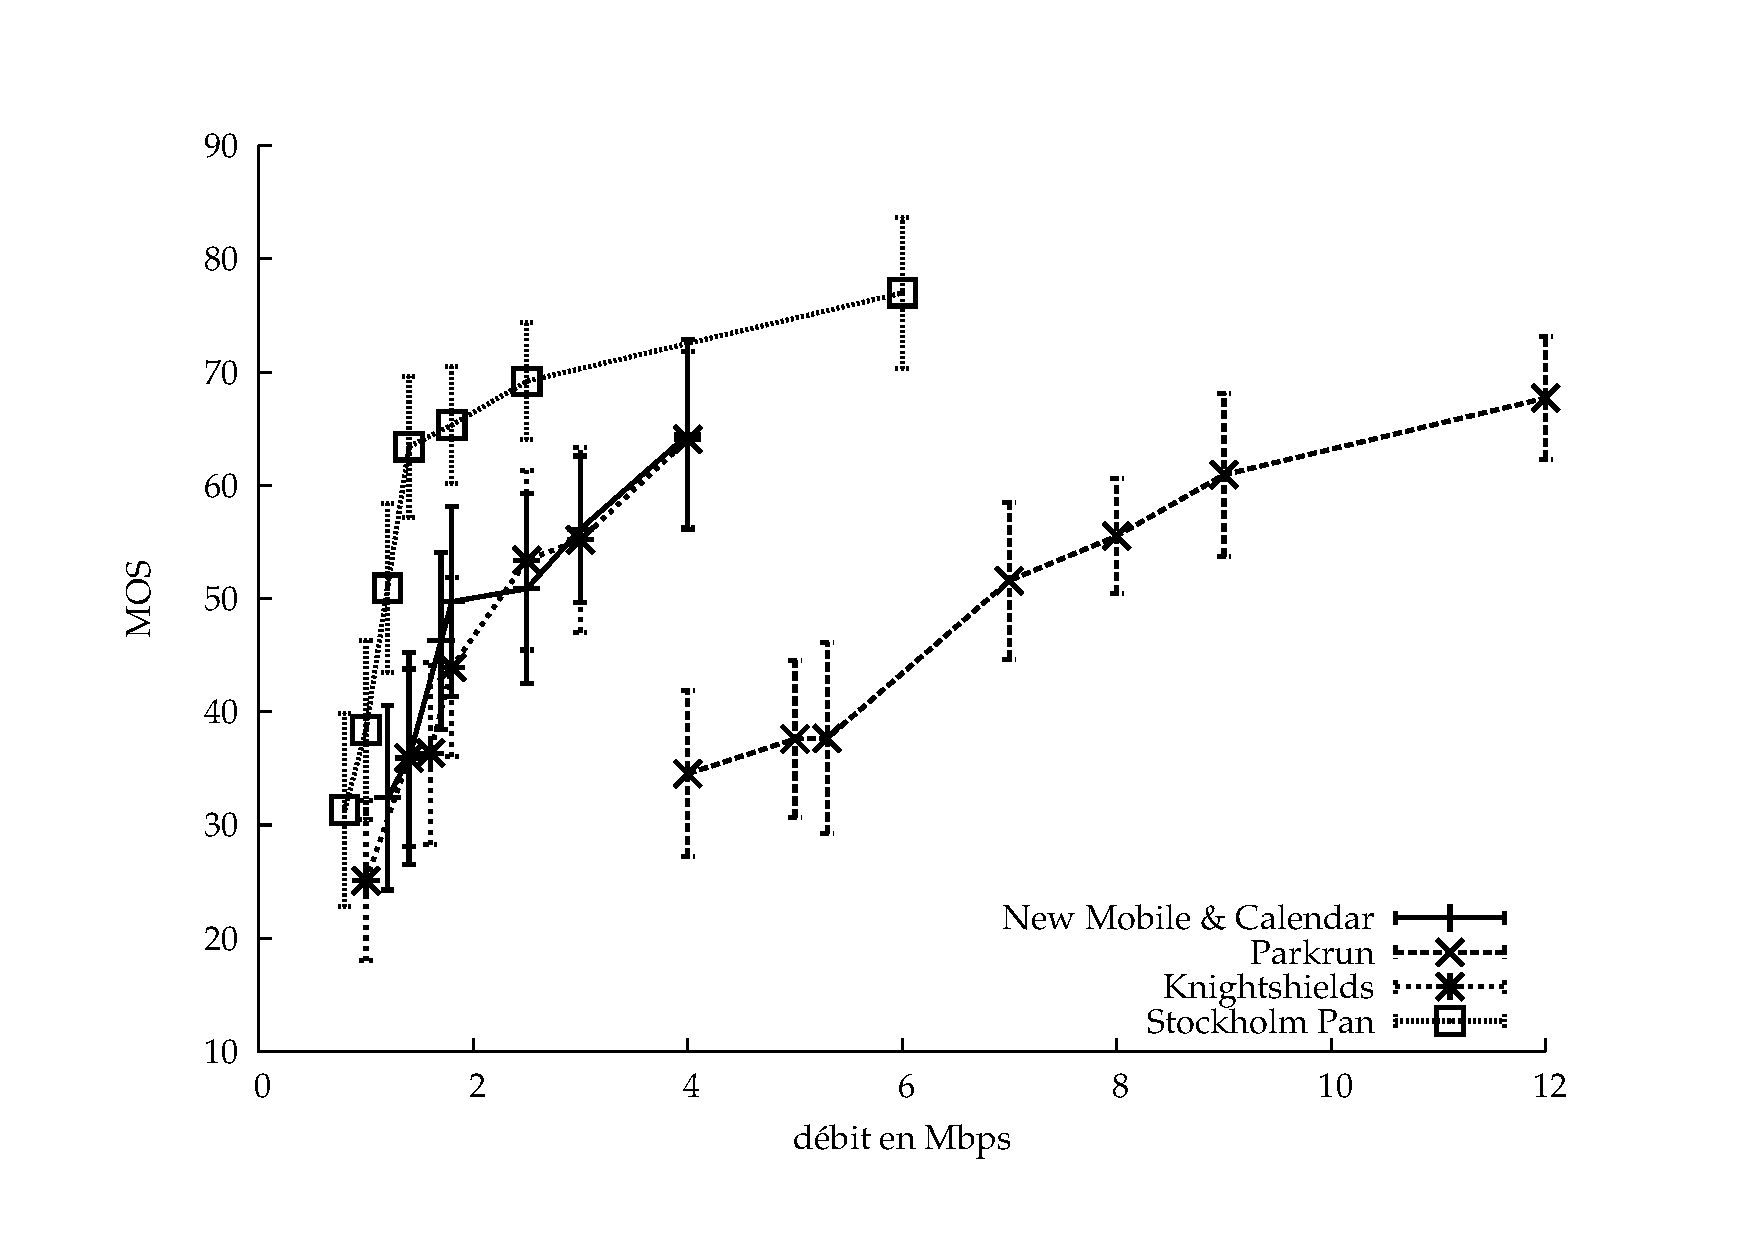
\includegraphics[page=1, width=0.9\linewidth, trim= 70 50 90 70]{plot/debit-mosSD}
\caption{Notes de qualité en fonction du débit, exprimé en Mbps, obtenues pour le codeur de référence H.264 par les séquences QHD.}
\label{fig:MOSrateCodeurRefSD}
\end{figure}

\begin{table}[htbp]
\centering
\begin{tabular}{cDDp{0.1cm}c} \toprule
\multirow{2}{2.5cm}{\strong{contenu}} & \multicolumn{2}{c}{\strong{MOS}} & & \multirow{2}{1.5cm}{$Q_b - Q_m$}\tabularnewline
\cmidrule{2-3}
 & $Q_m$ & $Q_b$ & \tabularnewline \toprule
\emph{New Mobile \& Calendar}	& 49,7 & 56,1 & & 6,4\tabularnewline \midrule
\emph{Parkrun}							& 37,7 & 60,9 & & 23,2\tabularnewline \midrule
\emph{Knightshields}					& 36,3 & 55,2 & & 18,9\tabularnewline \midrule
\emph{Stockholm Pan}				& 50,9 & 65,3 & & 14,4\tabularnewline \bottomrule
\end{tabular}
\caption{MOS des séquences compressées à des débits correspondant à des qualités moyenne et bonne en TVSD, et différence entre les deux qualités.}
\label{tab:bitratesSDQ60Q80}
\end{table}


\subsubsection{Description du protocole d'évaluation}
Le protocole conçu dérive de la méthodologie comparative avec jugement catégoriel décrite dans la recommandation ITU-R BT.500-11~\cite{itu-bt500-11} et présentée section~\ref{ssec:Méthode_avec_échelle_dévaluation_par_catégorie}. Dans notre cas, l'attribution des deux séquence, une au format HD et l'autre au format SD, est aléatoire. De plus, après une première visualisation, l'observateur peut revoir les séquences autant de fois qu'il le désire, c'est le principe d'accès aléatoire présent dans la méthodologie SAMVIQ~\cite{ebu-samviq}. C'est la principale modification au protocole classique de comparaison. Elle se justifie par la précision accrue qu'elle apporte, comme nous l'avons montré dans la section précédente.

Après la présentation, l'observateur doit rapporter sa préférence entre les deux contenus. Pour cela, il utilise l'échelle de comparaison présentée dans le tableau~\ref{tab:compscale}. Les valeurs numériques relevées ne sont jamais indiquées à l'observateur. De plus, les termes utilisés dans l'échelle évitent les connotations qualitatives. Ainsi, l'observateur rapporte sa préférence globale, et pas seulement la qualité visuelle. Les tests effectués consistent donc en la comparaison d'un ensemble de sept séquences HD avec un ensemble de deux séquences SD. Une session est donc composée de 14 présentations par contenu. %Il faut bien saisir la complexité de la tâche demandée aux observateurs. Il est toujours délicat de comparer des choses très différentes. C'est pour cela que lors de la séance préparatoire, il leur était précisément indiqué de noter selon leur préférence globale. Néanmoins, cette complexité entraine une dispersion inévitable. C'est la raison pour laquelle les intervalles de confiance sont relativement élevés.

\begin{table}[htbp]
\centering
\begin{tabular}{cc}\toprule
\textbf{préférence} & \textbf{valeur} \\ \toprule
Je préfère beaucoup plus A que B & +3 \\ \midrule
Je préfère plus A que B & +2 \\ \midrule
Je préfère un peu plus A que B & +1 \\ \midrule
Je n'ai pas de préférence & 0 \\ \midrule
Je préfère un peu moins A que B & --1 \\ \midrule
Je préfère moins A que B & --2 \\ \midrule
Je préfère beaucoup moins A que B & --3 \\ \bottomrule
\end{tabular}
\caption{Échelle de comparaison utilisée pour les tests de préférence entre télévision standard et télévision haute définition.}
\label{tab:compscale}
\end{table}


\subsection{Effets opposés de la taille de l'écran et des distorsions}
Pour évaluer la préférence moyenne entre TVHD et TVSD par rapport à leur différence de qualité, nous l'évaluons en fonction du $\Delta$MOS, calculé comme la différence entre le MOS de la TVHD et le MOS de la TVSD, pour chaque débit. Pour mieux comprendre le sens d'une telle représentation, la figure ~\ref{fig:lectureCourbesHDvsSD} délimite l'espace entre quatre quadrants, chacun ayant une signification précise. Les droites en pointillés sont particulièrement intéressantes. La verticale représente l'égalité des qualités TVHD et TVSD. L'horizontale représente l'isopréférence de l'observateur moyen entre TVHD et TVSD.

\begin{figure}[htbp]
\centering
\begin{tikzpicture}[scale=2.5]% comment lire les courbes HDvsSD

% \begin{tikzpicture}[scale=2]
	% The graphic
	\filldraw[draw=red!30,fill=red!30] (0,0) rectangle (2.5,1);
	\filldraw[draw=green!30,fill=green!30] (0,0) rectangle (-2.5,1);
	\filldraw[draw=blue!30,fill=blue!30] (0,0) rectangle (2.5,-1);
	\filldraw[draw=yellow!30,fill=yellow!30] (0,0) rectangle (-2.5,-1);

 	\draw[->] (-2.5,-1) -- (2.6,-1) node[below] {$\Delta$MOS} coordinate(x axis);
 	\draw[->] (-2.5,-1) -- (-2.5,1.2) node[above, text width=2cm, text centered] {préférence moyenne} coordinate(y axis);

	\draw (-2.6,0) node{0};
	\draw (0,-1.1) node{0};
	\draw[dotted] (-2.5,0) -- (2.5,0);
	\draw[dotted] (0,1) -- (0,-1);

	\draw (2.5,0.9) node[left] {HD préférée};
	\draw (2.5,0.7) node[left] {$MOS_{HD} > MOS_{SD}$};
	\draw (-2.5,0.9) node[right] {HD préférée};
	\draw (-2.5,0.7) node[right] {$MOS_{HD} < MOS_{SD}$};
	\draw (2.5,-0.9) node[left] {SD préférée};
	\draw (2.5,-0.7) node[left] {$MOS_{HD} > MOS_{SD}$};
	\draw (-2.5,-0.9) node[right] {SD préférée};
	\draw (-2.5,-0.7) node[right] {$MOS_{HD} < MOS_{SD}$};

	\draw (2.5,0.05) node[left, blue]{isopréférence};% (image size)};
	\draw (0,0) node[above, blue, rotate=90]{$MOS_{HD} = MOS_{SD}$};% (distortions)};
% \end{tikzpicture}
\end{tikzpicture}
\caption{Lecture des courbes de préférence entre TVHD et TVSD en fonction du $\Delta$MOS.}
\label{fig:lectureCourbesHDvsSD}
\end{figure}

% FIXME essayer de les placer sur la même page !

\begin{figure}[htbp]
\centering
\subfloat{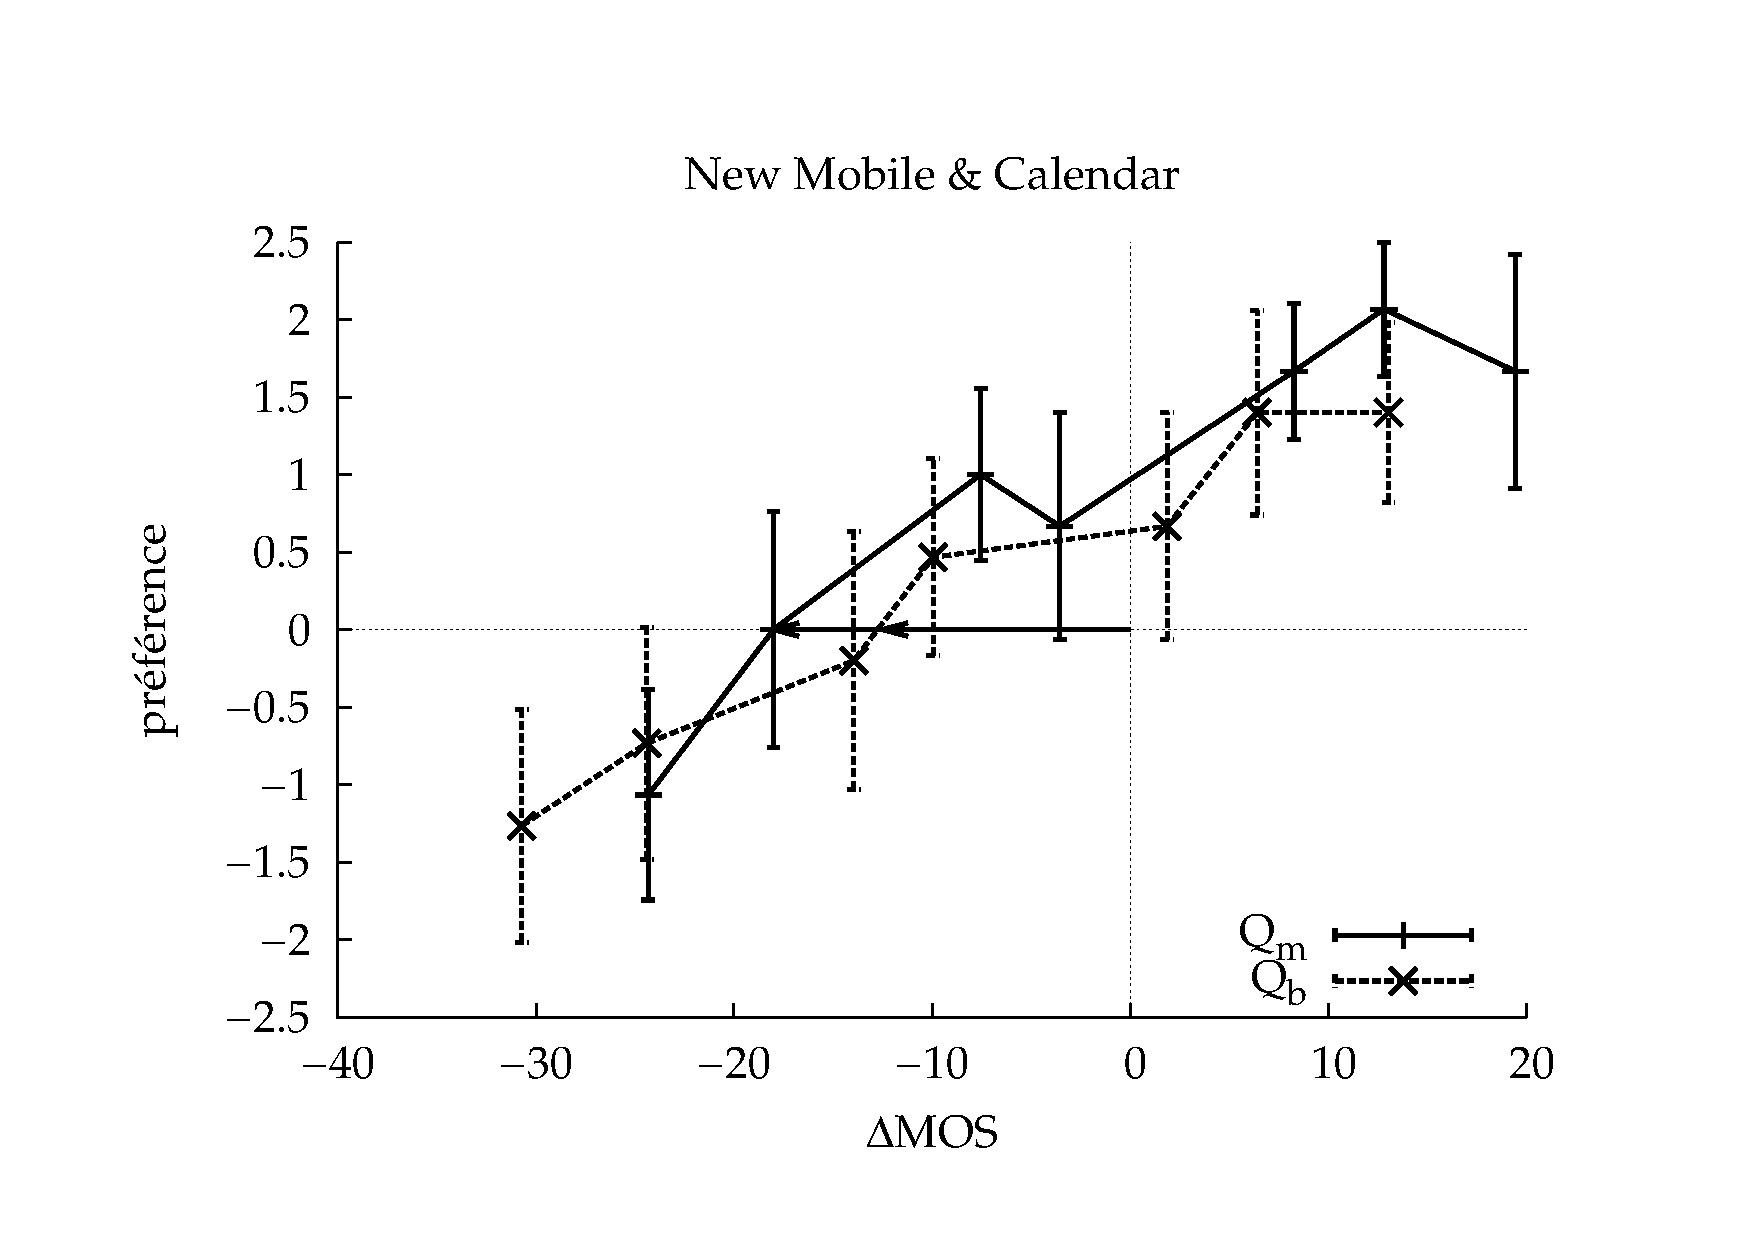
\includegraphics[page=1, width=0.48\linewidth, trim= 70 50 90 70]{plot/HDvsSD-LCD}}\hfill
\subfloat{\includegraphics[page=2, width=0.48\linewidth, trim= 70 50 90 70]{plot/HDvsSD-LCD}}\\
\subfloat{\includegraphics[page=3, width=0.48\linewidth, trim= 70 50 90 70]{plot/HDvsSD-LCD}}\hfill
\subfloat{\includegraphics[page=4, width=0.48\linewidth, trim= 70 50 90 70]{plot/HDvsSD-LCD}}\\
\caption{Préférence moyenne entre TVHD et TVSD en fonction du $\Delta$MOS pour quatre séquences SVT2002.}
\label{fig:HDvsSD-LCD}
\end{figure}

La figure~\ref{fig:HDvsSD-LCD} présente ces courbes pour les quatre contenus SVT2002. %De plus, elle présente les intervalles de confiance à 95\% calculés sur la préférence et sur les MOS.
Les flèches indiquent les valeurs $\Delta$MOS$_0$, prises à l'équilibre de la préférence entre TVHD et TVSD pour chaque contenu. Si $\Delta$MOS$_0$ est négatif, cela signifie que quand l'observateur moyen n'a pas de préférence entre les deux séquences, c'est celle au format HD qui a la moins bonne qualité. Le tableau~\ref{tab:DeltaMOS-MOShd-LCD} contient les valeurs de $\Delta$MOS$_0$ pour tous les contenus ainsi que le MOS de la version TVHD en ces points. Ce MOS$_{\HD}$ correspond à la qualité à partir de laquelle l'observateur moyen préfère la TVHD.%Les valeurs au passage à zéro ont été obtenues par interpolation linéaire.

\begin{table}[htbp]
\centering
\begin{tabular}{ccccc}\toprule
\multirow{2}{2.5cm}{\strong{contenu}} & \multicolumn{2}{c}{$Q_m$} & \multicolumn{2}{c}{$Q_b$}\tabularnewline
\cmidrule{2-5}
													& $\Delta$MOS$_0$ 	& MOS$_{\HD}$ 	& $\Delta$MOS$_0$ 	& MOS$_{\HD}$\\ \toprule
\emph{New Mobile \& Calendar}	& --18,0 						& 31,7					& --12,50						& 43,6\\ \midrule
\emph{Parkrun}							& --8,0 							& 29,6					& --18,0						& 42,9\\ \midrule
\emph{Knightshields}					& --1,8 							& 34,5					& 0								& 55,2\\ \midrule
\emph{Stockholm Pan}				& --12,0 						& 38,9					& --17.6						& 47,7\\ \bottomrule
\end{tabular}
\caption{$\Delta$MOS$_0$ et MOS$_{\HD}$ pour les qualités $Q_m$ et $Q_b$, et les quatre contenus SVT2002.}
\label{tab:DeltaMOS-MOShd-LCD}
\end{table}

Au vu du faible écart entre $Q_m$ et $Q_b$ pour le contenu \emph{New Mobile \& Calendar}, nous l'avons écarté de l'analyse. En effet, cela traduit le fait que l'observateur moyen fait une distinction de qualité insuffisante entre les deux séquences. La conséquence est que les préférences et les $\Delta$MOS sont proches les uns des autres.

Nous remarquons tout d'abord que lorsque la qualité de la TVHD décroit, la TVSD finit par être préférée à la TVHD, ce qui est le comportement attendu. En effet, à qualité TVSD constante, plus les dégradations introduites dans la TVHD vont gêner l'observateur et plus il va préférer l'autre version disponible.

Ensuite, les valeurs de $\Delta$MOS$_0$ sont toutes négatives ou nulles. Cela signifie que quand les observateurs n'ont pas de préférence particulière pour l'un ou l'autre des formats, la qualité intrinsèque de la TVSD est supérieure. De plus, cette supériorité est significative pour tous les contenus sauf \emph{Knightshields}. Cette différence de qualité en faveur de  la TVSD est compensée par la taille de l'image en TVHD. C'est ce que nous appelons l'\emph{effet grand écran}. L'observateur moyen est prêt à perdre un peu de qualité intrinsèque s'il peut bénéficier d'une image plus grande. La TVHD peut alors présenter plus de dégradations et obtenir la même préférence que la TVSD.

Ceci est d'autant plus vrai que $\Delta$MOS$_0$ est négatif. Or en dehors de la séquence \emph{New Mobile \& Calendar} que nous avons écarté, nous avons toujours $\Delta$MOS$_0(Q_m) > \Delta$MOS$_0(Q_b)$. Ainsi, quand la TVHD est comparée à une TVSD de bonne qualité $Q_b$, l'effet grand écran est prédominant. L'observateur moyen tire avantage de la taille de l'écran pour profiter pleinement de la TVHD.

Par contre, quand la TVHD est comparée à une TVSD de qualité moyenne $Q_m$, cet effet décroit. Les valeurs de $\Delta$MOS$_0$ croissent significativement, sauf pour \emph{Knightshields} pour qui les valeurs ne sont pas significativement différentes. Ainsi, quand les observateurs n'ont pas de préférence particulière entre les qualités de la TVHD et de la TVSD, leurs qualités intrinsèques sont plus proches. Cela signifie que l'effet grand écran perd ici de son influence au profit de l'impact des dégradations même de la séquence. Celle-ci est tellement dégradée que l'observateur moyen tend à préférer la TVSD car subir des distorsions sur une petite image est moins gênant que sur une grande. Ici, l'effet des dégradations est prédominant dans l'élaboration de la préférence de l'observateur.

Ceci fournit une information de première importance pour les diffuseurs de télévision haute définition. La TVHD doit être de qualité significativement supérieure afin de tirer tout le bénéfice de l'effet grand écran et non pas le transformer en déficit. %La qualité visuelle en TVHD doit donc être assurée pour que les usagers trouve un intérêt au passage à cette nouvelle technologie.


\subsection{Conclusion}
Cette section a permis de déterminer la préférence de l'observateur moyen entre la télévision haute définition et la télévision standard. L'étude menée a consisté à comparer directement les deux formats lors de tests subjectifs. Pour cela, un protocole et une méthodologie de visualisation simultanée des deux formats ont été conçus. Ces tests ont donc été réalisés avec d'un côté le respect maximal des recommandations en terme de conditions expérimentales, et de l'autre, la nécessité de définir de nouvelles propriétés à des tests sans précédent dans la littérature.

L'enseignement de cette étude est que l'observateur moyen doit composer avec deux effets contradictoires. D'un côté, il peut bénéficier d'une plus grande image et donc d'une meilleure qualité visuelle. De l'autre, il peut subir des dégradations importantes dues au codage \avc, ce qui fait chuter cette même qualité visuelle. Afin de la conserver à un haut niveau et donc de satisfaire l'observateur, un service de TVHD doit donc assurer une qualité visuelle de haut niveau. L'exploitation intéressante de la haute définition doit être liée à une faible quantité de dégradations visibles.


\section{Impact de l'affichage sur la qualité} \label{sec:Études_Impact_Affichage_Qualité}
La transition vers la haute définition s'accompagne d'une modification des techniques d'affichage. Cela a évidemment un impact sur la qualité d'image que nous cherchons à évaluer. Nous nous intéressons à l'effet lié aux technologies CRT et LCD, qui sont techniquement très différentes. Les avantages du LCD sont son encombrement réduit et sa plus grande gamme de luminosité. Cependant, le temps de réponse de l'écran et les défauts de restitution des zones sombres et du mouvement ont un impact important sur la perception de la qualité. Le mouvement sur un écran LCD est accompagné d'un flou caractéristique. Celui-ci est dû à la manière dont l'image est affichée. Dans la technologie CRT, une image est affichée par un balayage pixel par pixel. Ainsi, l'image n'est pas maintenue entre deux balayages successifs. La persistance rétinienne permet de créer un mouvement apparent grâce à la grande vitesse de balayage. Par contre,  sur un écran LCD, les pixels sont affichés tous ensemble et l'image est maintenue affichée en attendant la suivante. Or, pour un contenu en mouvement, l'\oe il humain a naturellement tendance à le suivre au cours du temps. Ce suivi, combiné au maintien de l'image sur l'écran, entraine l'intégration temporelle de l'objet sur la rétine, ce que l'observateur ressent comme du flou. Les figures~\ref{fig:integrationLCD} et~\ref{fig:integrationCRT} illustrent ces principes. Ce défaut majeur a été étudié par Sylvain Tourancheau~\cite{tourancheau-vpqm2007, tourancheau-icip2007}. Il a notamment montré l'impact de la définition sur la différence de perception de la qualité entre un écran CRT et un écran LCD.

\begin{figure}[htbp]
	\centering
	\subfloat[\label{fig:integrationLCD} Perception d'un objet en mouvement avec un écran LCD.]{\begin{tikzpicture}[scale=1.4]\filldraw[fill=blue!30] (0,0.5) rectangle (1,1.5);
\filldraw[fill=blue!30] (1,0.8) rectangle (2,1.8);
\filldraw[fill=blue!30] (2,1.1) rectangle (3,2.1);

\draw[->] (0,0) -- (4,0) node[below] {temps} coordinate(x axis);
\draw[->] (0,0) -- (0,2.5) node[above] {espace} coordinate(y axis);
\draw (0, -0.2) node{$i$};
\draw (1,-0.2) node{$i+1$};
\draw (1,0) -- (1,0.1);
\draw (2,-0.2) node{$i+2$};
\draw (2,0) -- (2,0.1);
\draw (3,-0.2) node{$i+3$};
\draw (3,0) -- (3,0.1);

\draw[help lines,->] (0,1.5) -- (4,2.7);
\draw[help lines,->] (0,0.2) -- (4,1.4);

\filldraw[fill=blue!30] (4,2.7) -- (4,1.4) -- (4.2,1.75) -- (4.2,2.45) -- cycle;
\draw[help lines,dashed] (0,0.5) -- (4.5,1.85);
\draw[help lines,dashed] (0,1.2) -- (4.5,2.55);

\draw (4,3) -- (4,1) node[below]{intégration};
\end{tikzpicture}}\hfill
	\subfloat[\label{fig:integrationCRT} Perception d'un objet en mouvement avec un écran CRT.]{\begin{tikzpicture}[scale=1.4]\filldraw[fill=blue!30] (0,0.5) rectangle (0.05,1.5);
\filldraw[fill=blue!30] (1,0.8) rectangle (1.05,1.8);
\filldraw[fill=blue!30] (2,1.1) rectangle (2.05,2.1);

\draw[->] (0,0) -- (4,0) node[below] {temps} coordinate(x axis);
\draw[->] (0,0) -- (0,2.5) node[above] {espace} coordinate(y axis);
\draw (0, -0.2) node{$i$};
\draw (1,-0.2) node{$i+1$};
\draw (1,0) -- (1,0.1);
\draw (2,-0.2) node{$i+2$};
\draw (2,0) -- (2,0.1);
\draw (3,-0.2) node{$i+3$};
\draw (3,0) -- (3,0.1);

\draw[help lines,->] (0,1.5) -- (4,2.7);
\draw[help lines,->] (0,0.5) -- (4,1.7);

\filldraw[fill=blue!30] (4,2.7) -- (4,1.7) -- (4.2,1.75) -- (4.2,2.65) -- cycle;
\draw (4,3) -- (4,1.4) node[below]{intégration};
\end{tikzpicture}}\\
	\caption{Comparaison de la perception d'un objet en mouvement avec un écran LCD et CRT.}
\end{figure}

Le second effet est lié au type de méthodologie utilisée dans le redimensionnement d'image. En effet, alors que les écrans de TVHD ont tous une définition supérieure à celle de la TVSD, ils devront, pendant une période, être capable d'afficher des images dans les deux définitions. Or, ce traitement a un cout en termes de qualité d'image et nous voulons mesurer cette perte. Dans le but d'évaluer l'impact du type de technologie d'affichage, des tests ont été réalisés à la fois sur l'écran LCD et sur l'écran CRT. Parmi ceux-ci, nous en avons effectué sur des séquences de définition QHD, QHD redimensionnée et TVHD afin d'évaluer l'impact de l'adaptation de l'image à une certaine définition.


\subsection{Impact du type de technologie d'affichage} \label{ssec:impactTechnoAffichage}
La figure~\ref{fig:nuageMOSCRTLCD} présente les MOS mesurés sur écran LCD en fonction des MOS mesurés sur écran CRT pour 96 séquences de TVHD. La droite pointillée correspond à l'égalité des MOS. Le coefficient de corrélation linéaire entre les deux ensembles de données est de 0,950. Cela montre la bonne cohérence des deux évaluations. Il existe donc une relation forte entre les deux ensembles de MOS. Il est possible de définir une fonction de transformation de l'un à l'autre comme l'a fait Tourancheau~\cite{tourancheau-vpqm2007}. Cependant, le nuage de points montre une nette supériorité pour le CRT. En effet, les qualités mesurées sur le CRT sont, à quelques exceptions près, toujours supérieures à celles mesurées sur le LCD. La racine carrée de l'erreur quadratique moyenne reqm par contenu est présentée dans le tableau~\ref{tab:diffMOS}.

\begin{figure}[htbp]
	\centering
	\begin{tikzpicture}[only marks, scale=0.07]
		\pgfsetplotmarksize{1.5cm}
		\draw plot[mark=+] file {plot/chap2/MOS-LCD-CRT.txt};
		\draw[->] (0,0) -- node[below=0.5cm] {MOS sur CRT} (95,0);
		\draw[->] (0,0) -- node[above=0.7cm, sloped] {MOS sur LCD} (0,95) ;
		\foreach \x in {0,15,30,45,60,75,90} \draw (\x,1) -- (\x,-1) node[anchor=north] {\x};
		\foreach \y in {0,15,30,45,60,75,90} \draw (1,\y) -- (-1,\y) node[anchor=east] {\y};
		\draw[dotted] (0,0) -- (90,90);
	\end{tikzpicture}
	\caption{MOS LCD en fonction des MOS CRT pour 96 séquences.}
	\label{fig:nuageMOSCRTLCD}
\end{figure}

\begin{table}[htbp]
\centering
\begin{tabular}{cc}\toprule
\textbf{séquence}						& \textbf{reqm}	\\ \toprule
\emph{New Mobile \& Calendar}	& 12,47	\\\midrule
\emph{Parkrun}							& 10,02	\\\midrule
\emph{Knightshields}					& 11,69	\\\midrule
\emph{Stockholm Pan}				& 8,60		\\\midrule
\emph{Concert}							& 12,07	\\\midrule
\emph{Foot}								& 16,38	\\\midrule
\emph{Movie}								& 18,49	\\\midrule
\emph{Voile}								& 14,87	\\\midrule
\emph{Crédits}							& 16,68	\\\midrule
\emph{Golf}									&  9,72		\\\midrule
\emph{Show}								& 14,99	\\\midrule
\emph{Standing}							& 16,17	\\\bottomrule
\end{tabular}
\caption{Racine carrée de l'erreur quadratique moyenne entre les qualités subjectives mesurées sur écran CRT et sur écran LCD pour chaque séquence SVT2002 et Euro1080.}
\label{tab:diffMOS}
\end{table}

Les plus fortes valeurs correspondent aux contenus \emph{Foot}, \emph{Movie}, \emph{Crédits} et \emph{Standing}. Les plus faibles correspondent à \emph{Stockholm Pan} et \emph{Golf}. Les origines de ces valeurs extrêmes sont variées. Foot se distingue par un fort mouvement d'ensemble dans la séquence. Il en est de même pour \emph{Crédits} où, en plus, du texte défile de bas en haut. Or, nous savons que le flou de mouvement est un des défauts majeurs de l'affichage LCD. Par contre, \emph{Movie} est très statique et présente un concert dans une cathédrale filmé de haut. \emph{Standing} est également très statique et ne présente qu'un orateur en plan rapproché poitrine. L'attention de l'observateur, non captée par une scène à si faible contenu informatif, se détourne rapidement pour détecter les dégradations, notamment dans les nombreuses zones sombres présentes autour de l'orateur. Le rendu de ces zones sombres est également un défaut connu de la technologie LCD. À l'opposé, \emph{Stockholm Pan} et \emph{Golf} sont des séquences très statiques et lumineuses. La première est un panorama de la ville de Stockholm en pleine journée. La seconde est un plan sur des joueurs de golf avec un fort ensoleillement. Avec ce type de contenu, l'écran LCD fournit une bonne qualité d'image.

Ces résultats illustrent donc l'impact de la technologie d'affichage utilisée. Cela a son importance et les constructeurs d'écran l'ont bien compris, puisque tous les écrans actuels incorporent de nombreux post-traitements, toujours en nombre croissant. De plus, cette étude confirme les résultats de celle de l'ITU~\cite{itu-crtlcd} présentée en \ref{ssec:itu}. Cependant cette fois-ci, nous utilisons deux écrans de résolution native 1920\texttimes1080, ce qui n'introduit pas de biais supplémentaire.


\subsection{Impact de l'adaptation de l'image à une définition supérieure}
Lors de l'affichage d'une image de TVSD sur un écran de TVHD, une technique de sur-échantil\-lon\-nage doit être utilisée. Celle-ci engendre des dégradations visibles. Pour déterminer la perte de qualité provoquée, nous avons évalué la qualité de séquences sur-échantillonnées. Les séquences au format QHD crées dans la section précédente ont subit un tel traitement. Le résultat de ce traitement est nommé TVHD'. L'algorithme Lanczos3, très utilisé et réputé dans le domaine du redimensionnement, est appliqué sur ces 28 séquences et les quatre contenus correspondants. Cette méthode d'interpolation est définie sur une fenêtre comme un produit de fonctions sinus cardinal normalisées. Le noyau obtenu est utilisé pour convoluer l'image à retailler. L'approximation effectuée est fonction de la taille de la fenêtre utilisée. La figure~\ref{fig:TVHD2QHD2TVHDp} présente le schéma de création de chaque type de séquence à partir de de la source TVHD.

\begin{figure}[htbp]
	\centering
	\begin{tikzpicture}[text centered, text width=3em, node distance = 2.5cm]
	\node (tvhd) {TVHD};
	\node[action, right of=tvhd, text width=5em] (filtre) {filtre demi-bande};
	\node[action, right of=filtre] (down) {$\downarrow$ 2};
	\node[right of=down] (qhd) {QHD};
	\node[action, right of=qhd, text width=5em] (up) {$\uparrow$ 2 Lanczos3};
	\node[right of=up, text width=3.2em] (tvhdp) {TVHD'};
	\path [fleche] (tvhd) -- (filtre);
	\path [fleche] (filtre) -- (down);
	\path [fleche] (down) -- (qhd);
	\path [fleche] (qhd) -- (up);
	\path [fleche] (up) -- (tvhdp);
	\end{tikzpicture}
	\caption{Schéma de création des séquences QHD et TVHD' à partir des séquences TVHD.}%
	\label{fig:TVHD2QHD2TVHDp}%
\end{figure}

La qualité des séquences TVHD' est mesurée dans les mêmes conditions d'expérimentation que pour les séquences de TVHD et de QHD. Les figures~\ref{fig:HD-SDup-LCD} et~\ref{fig:SD-SDup-LCD} présentent respectivement les MOS des séquences de TVHD' en fonction des MOS des séquences de QHD et des MOS des séquences de TVHD originales mesurés sur un écran LCD. Les figures~\ref{fig:HD-SDup-CRT} et~\ref{fig:SD-SDup-CRT} présentent respectivement les MOS des séquences de TVHD' en fonction des MOS des séquences de QHD et des MOS des séquences de TVHD originales mesurés sur un écran CRT.

\begin{figure}[htbp]
	\centering
\subfloat[\label{fig:HD-SDup-LCD}MOS des séquences de TVHD' en fonction des MOS des séquences de TVHD sur LCD.]{
	\begin{tikzpicture}[only marks, scale=0.09]
		\pgfsetplotmarksize{1cm}
		\draw plot[mark=+] file {plot/chap2/HD-SDup-LCD.txt};
		\draw[->] (20,20) -- node[below=0.5cm] {MOS TVHD} (85,20);
		\draw[->] (20,20) -- node[above=0.7cm, sloped] {MOS TVHD'} (20,85) ;
		\foreach \x in {20,40,60,80} \draw (\x,21) -- (\x,19) node[anchor=north] {\x};
		\foreach \y in {20,40,60,80} \draw (21,\y) -- (19,\y) node[anchor=east] {\y};
		\draw[dotted] (20,20) -- (80,80);
	\end{tikzpicture}}\hfill
\subfloat[\label{fig:SD-SDup-LCD}MOS des séquences de TVHD' en fonction des MOS des séquences de QHD sur LCD.]{
	\begin{tikzpicture}[only marks, scale=0.09]
		\pgfsetplotmarksize{1cm}
		\draw plot[mark=+] file {plot/chap2/SD-SDup-LCD.txt};
		\draw[->] (20,20) -- node[below=0.5cm] {MOS QHD} (85,20);
		\draw[->] (20,20) -- node[above=0.7cm, sloped] {MOS TVHD'} (20,85) ;
		\foreach \x in {20,40,60,80} \draw (\x,21) -- (\x,19) node[anchor=north] {\x};
		\foreach \y in {20,40,60,80} \draw (21,\y) -- (19,\y) node[anchor=east] {\y};
		\draw[dotted] (20,20) -- (80,80);
	\end{tikzpicture}}\\
	\subfloat[\label{fig:HD-SDup-CRT}MOS des séquences de TVHD' en fonction des MOS des séquences de TVHD sur CRT.]{
	\begin{tikzpicture}[only marks, scale=0.09]
		\pgfsetplotmarksize{1cm}
		\draw plot[mark=+] file {plot/chap2/HD-SDup-CRT.txt};
		\draw[->] (20,20) -- node[below=0.5cm] {MOS TVHD} (85,20);
		\draw[->] (20,20) -- node[above=0.7cm, sloped] {MOS TVHD'} (20,85) ;
		\foreach \x in {20,40,60,80} \draw (\x,21) -- (\x,19) node[anchor=north] {\x};
		\foreach \y in {20,40,60,80} \draw (21,\y) -- (19,\y) node[anchor=east] {\y};
		\draw[dotted] (20,20) -- (80,80);
	\end{tikzpicture}}\hfill
	\subfloat[\label{fig:SD-SDup-CRT}MOS des séquences de TVHD' en fonction des MOS des séquences de QHD sur CRT.]{
	\begin{tikzpicture}[only marks, scale=0.09]
		\pgfsetplotmarksize{1cm}
		\draw plot[mark=+] file {plot/chap2/SD-SDup-CRT.txt};
		\draw[->] (20,20) -- node[below=0.5cm] {MOS QHD} (85,20);
		\draw[->] (20,20) -- node[above=0.7cm, sloped] {MOS TVHD'} (20,85) ;
		\foreach \x in {20,40,60,80} \draw (\x,21) -- (\x,19) node[anchor=north] {\x};
		\foreach \y in {20,40,60,80} \draw (21,\y) -- (19,\y) node[anchor=east] {\y};
		\draw[dotted] (20,20) -- (80,80);
	\end{tikzpicture}}\\
	\caption{Comparaison des MOS des séquences QHD, TVHD' et TVHD sur un écran CRT et un écran LCD.}
\end{figure}

Il est clair que l'adaptation de l'image à une définition supérieure a un impact sur la qualité perçue. Dans les quatre comparaisons, les séquences ayant subi un redimensionnement ont une qualité nettement inférieure. Il est logique que la comparaison avec la TVHD soit à l'avantage de celle-ci. Le traitement ne peut retrouver la qualité originale perdue dans le sous-échantil\-lon\-nage. La perte est sensible, surtout dans les hautes qualités. La différence est moins prononcée dans les qualités basses, ce qui est dû aux dégradations. Celles-ci sont alors particulièrement visibles et gênantes et l'impact du redimensionnement y est moins important. Néanmoins, les applications de TVHD situent leur gamme dans les hautes et très hautes qualités, c'est donc dans ces gammes qu'il faut être performant.

Sur écran LCD, les MOS des séquences de TVHD et ceux des séquences de TVHD' montrent un coefficient de corrélation linéaire de 0,940 et une racine carrée de l'erreur quadratique moyenne de 13,73. Malgré la nette différence en faveur de la TVHD, les MOS conservent une relation forte. Sur écran CRT, le coefficient de corrélation chute à 0,839 et la racine carrée de l'erreur quadratique moyenne vaut 16,50. La relation est beaucoup moins importante et l'erreur s'accroit. Nous savons que les MOS mesurés sur CRT sont plus élevés que sur LCD. Si la corrélation chute sur cet écran, cela renforce l'importance de l'écart entre TVHD et TVHD'.

Plus étonnant, la différence de qualité entre la version TVHD' et la version QHD est approximativement du même ordre que celle entre la version TVHD' et la version de TVHD. En effet la racine carrée de l'erreur quadratique moyenne est de 12,80 sur l'écran LCD et de 14,61 sur l'écran CRT. Dans ce cas, bien que les observateurs bénéficient d'une grande image, l'impact du traitement de redimensionnement est tel qu'ils attribuent une meilleure qualité à la version non traitée. De plus, sur écran LCD, les MOS des séquences de QHD et ceux des séquences de TVHD' produisent un coefficient de corrélation linéaire de 0,960. Sur écran CRT, il chute à 0,906. Bien que moins importante, nous constatons la même chute que pour la comparaison entre TVHD et TVHD'.

Pour les services de TVHD, cela signifie qu'un écran ne gagne pas en qualité à étirer l'image à la taille de la dalle. Néanmoins, les technologies d'affichage moderne incluent des traitements permettant d'atténuer les dégradations dues à cet étirement. Nous n'en avons pas évalué, mais il nous apparait ici comme évident que ce type de traitements est indispensable.


\subsection{Conclusion} % TODO réflexion de fond à mener
Nous tirons deux conclusions majeures de cette section. Tout d'abord, nous avons montré la différence de qualités visuelles mesurées sur deux écrans de différentes technologies. Les MOS mesurés sur un écran de type CRT sont significativement supérieurs à ceux mesurés sur un écran de type LCD. Cependant, cette conclusion doit être relativisée par le fait que l'écran CRT était un matériel professionnel et que l'écran LCD était utilisé sans aucun post-traitement d'affichage. %Le but est donc uniquement de comparer les technologies d'affichage.

Nous nous sommes aussi intéressés à l'impact du redimensionnement d'image pour l'affichage. Celui-ci est couramment utilisé dans les téléviseurs modernes. Ce type de traitement a évidemment un impact négatif sur la qualité comparée à la qualité originale de la TVHD. Il est plus surprenant de constater qu'un écart important est mesuré quand ces séquences redimensionnées sont comparées avec les séquences de définition standard. Bien que permettant un effet grand écran artificiel, cette pratique est destructrice de qualité, et son utilisation seule n'apporte rien à l'utilisateur final.


\section{Conclusion}
Plusieurs aspects de la qualité visuelle en télévision haute définition ont été étudiés. Nous avons d'abord définit clairement la notion de qualité d'usage que nous avons réduit à la qualité visuelle. Trois aspects ont par la suite été développés. Concernant l'impact de la méthodologie d’évaluation subjective de la qualité, nous avons montré :
\begin{itemize}
\item que les méthodologies ACR et SAMVIQ ne fournissent pas des mesures de qualités similaires en TVHD, le choix de l'une ou l'autre doit donc être fait en connaissance de cause ;
\item que la taille de l'image, et donc celle du champ visuel excité, a une influence sur l'évaluation de qualité, ce qui explique une chute du coefficient de corrélation entre les évaluations produites par les méthodologies ACR et SAMVIQ en TVHD ;
\item qu'à nombre d'observateurs identique, la méthodologie SAMVIQ fournit des MOS de plus grande précision que la méthodologie ACR.
\end{itemize}

Dans la suite de nos travaux, la méthodologie SAMVIQ sera privilégiée. Elle a ainsi permis d'évaluer la qualité sur une base importante de 192 séquences TVHD. Les résultats de cette évaluation sont utilisés dans une étude de préférence entre la télévision haute définition et télévision standard. Dans cette étude, nous avons :
\begin{itemize}
\item conçu une méthodologie de comparaison visuelle de contenus à plusieurs définitions ;
\item identifié deux effets contradictoires avec lesquels l'observateur moyen doit composer lorsqu'il passe de la TVSD à TVHD, à savoir la taille de l'écran et la quantité de dégradations contenue ;
\item déterminé les zones d'influence de ces deux effets ;
\item montré que le gain en qualité visuelle de la télévision haute définition est directement lié à une faible quantité de dégradations perçues.
\end{itemize}

Enfin, nous avons évalué l'impact de l'affichage sur la qualité. Pour cela, nous avons d'une part effectué des tests à la fois sur écran LCD et sur écran CRT. D'autre part, nous avons évalué des séquences vidéos à différentes définitions, ayant subit pour cela un redimensionnement de taille. Ceci a permis :
\begin{itemize}
\item de montrer que la différence de technologie d'affichage introduit un biais de qualité en faveur de l'écran CRT ;
\item de constater que les techniques de redimensionnement d'image provoquent des pertes de qualité sensibles.
\end{itemize}

L'ensemble de ces contributions nous a permis de mieux comprendre l'impact de la télévision haute définition sur la qualité visuelle. Les changements que cette nouvelle technologie implique sont nombreux et nécessitent des précautions quant à leur utilisation par les usagers. Ceux-ci doivent bénéficier d'une qualité visuelle sensiblement supérieure afin d'assurer le succès du système. Dans cette optique, il peut être intéressant de connaitre l'impact des dégradations de type codage sur la qualité visuelle. C'est l'objet du prochain chapitre.


\ornementChapitre

% %%%%%%%%%%%%%%%%%%%%%%%%%%%%%%%%%%%%%%%%%%%%%%%%%
%%%
%%% Auteur : Stéphane Péchard - stephane.pechard@univ-nantes.fr
%%% Fichier : 6-methode.tex - sixième chapitre : Méthode des tubes
%%% Version : 0.1
%%% Date : 2007/07/30
%%%
%%%%%%%%%%%%%%%%%%%%%%%%%%%%%%%%%%%%%%%%%%%%%%%%%
\chapter{Méthodologie d'évaluation subjective de l'impact d'un système dégradant sur la qualité visuelle} \label{chap:methode}
% \opt{final}{\lettrine[lines=4]{D}{iffuser de la télévision haute définition}}\opt{nofinal}{Diffuser de la télévision haute définition} nécessite le transport d'une très grande quantité d'information. À la base, sans faire appel aux techniques de compression d'information, celle-ci est multipliée par cinq par rapport à la TVSD. C'est pourquoi la compression est indispensable à la mise à disposition d'un tel service. Le débit de la TVHD 1080i avant compression est d'environ 800 Mbps, rien que pour la vidéo. Parallèlement, les débits visés pour la diffusion de la TVHD sont de l'ordre de 10 Mbps. Il faut donc réduire de façon très importante la quantité d'information à transmettre d'un facteur d'au moins 80. En pratique, un facteur 100 est visé. La première génération de TVHD actuellement utilisée aux États-Unis ou au Japon utilise la norme de compression MPEG-2. Pour sa généralisation en Europe, il est prévu d'utiliser la norme \avc, aussi appelée MPEG-4/Advanced Video Coding. Plus récente et plus performante, celle-ci permet de diviser les débits MPEG-2 par deux à qualité visuelle équivalente. Évidemment, une telle compression des données affecte quelque peu le rendu visuel. En effet, les techniques de compression sans perte ne réduisent le débit que d'un facteur deux environ, taux de compression très insuffisant. Il faut se résoudre à utiliser, comme le fait MPEG-2, des techniques de compression avec pertes. Vu les taux de compression utilisés, les distorsions dues à la compression deviennent visibles. La qualité visuelle de l'image est donc affectée. La perte d'information est alors perçue par l'observateur sous la forme d'apparition de phénomènes dégradants spatiaux et temporels non réalistes.

% Mesurer ces dégradations permet d'en déterminer l'impact sur la qualité visuelle. Or, pour un débit donné, le but d'un système moderne de compression d'information est de minimiser les dégradations qu'il génère. Il semblerait donc logique de pouvoir calculer la quantité de dégradations en fonction du débit et utiliser cette relation pour déterminer la qualité perçue correspondant à un certain débit. Ce n'est malheureusement pas aussi élémentaire. En effet, la relation entre la qualité ressentie et le niveau des dégradations n'est pas simple du fait de la diversité des dégradations mais aussi et surtout car elle fait intervenir un élément très complexe : le jugement humain. Nous remarquons que les systèmes de codage n'optimisent pas leurs procédés selon l'impact que ceux-ci peuvent avoir sur le jugement humain mais plutôt selon des paramètres statistiques élémentaires basés sur des différences entre signaux numériques d'entrée et de sortie. Or, il est connu que les appréciations issues du jugement humain et ces paramètres statistiques élémentaires ne sont pas très corrélées.

\opt{final}{\lettrine[lines=4]{I}{l existe plusieurs approches pratiques possibles}}\opt{nofinal}{Il existe plusieurs approches pratiques possibles} pour mesurer de manière subjective les dégradations générées par un système dégradant. Celles que nous avons présentées dans le premier chapitre étaient globales, c'est-à-dire qu'elles considéraient la séquence dans son entier et que le système dégradant s'appliquaient entièrement sur la séquence. Nous proposons ici une approche plus fine. Il existe d'autres méthodes adoptant une approche fine~\cite{farias-phd,eusipco2006-wolff} mais elles utilisent une classification des dégradations présentes dans la séquence. Ce type de méthode suppose une mesure indépendante de chaque dégradation, ce qui n'est pas sans soulever quelques problèmes pratiques.

Dans ce chapitre, nous présentons une méthodologie permettant d'estimer l'impact de dégradations de codage sur la qualité perçue par l'observateur moyen. L'approche envisagée s'inspire des travaux de Farias~\cite{farias-phd}. Cependant, nous préférons ne pas considérer plusieurs types de dégradations qui seraient appliqués arbitrairement sur tout ou partie d'une séquence vidéo. Nous renversons cette approche en considérant un unique type de dégradation provenant du codage, au lieu d'une liste de dégradations qu'il est difficile de déterminer étant donné la diversité des conséquences visibles d'un processus de compression. Dans un second temps, nous exploiterons la méthodologie pour rechercher une éventuelle relation entre les pertes de qualité locales et la perte de qualité globale. %Cependant, nous considérons que cette dégradation s'applique de manière différente suivant l'activité spatio-temporelle locale du contenu. Nous passons donc d'un partitionnement des dégradations en type à un partitionnement du contenu en zones spatio-temporelles. Pour cela, nous proposons une méthode de classification spatio-temporelle d'un contenu vidéo. Chaque partie obtenue est ensuite dégradée et évaluée indépendemment. Dans notre contexte, nous restreignons notre étude aux dégradations introduites pas le système de codage \avc. Une fois que nous disposons des pertes de qualité de chaque type de contenu, nous essayons de savoir si il est possible de les relier avec la perte de qualité globale. Un tel résultat serait très intéressant dans l'optique d'un critère objectif de qualité. Dans un second temps, nous cherchons à créer un paramètre de contrôle de dégradation par type de contenu. Celui-ci permet alors de construire un modèle de perte de qualité basé sur une fonction de gêne.


\section{Vers une classification du contenu et non des dégradations}
Avant de décrire notre méthode de classification spatio-temporelle et de l'exploiter, nous commençons par détailler l'approche proposée par Farias, dont nous nous inspirons. Elle utilise sa méthode pour mesurer les dégradations présentes dans une vidéo codée par MPEG-2 et créer des critères objectifs de qualité. Nous expliciterons ensuite les défauts dans la réalisation de la méthode et les modifications que nous nous proposons d'y apporter afin de mieux répondre à la problématique.


\subsection{Approche de Farias}
Farias~\cite{farias-phd} propose de considérer une liste de dégradations et de tester leur influence sur la qualité perçue suivant la tâche demandée à l'observateur. La figure~\ref{fig:approcheFarias} présente une schématisation simplifiée de cette approche. Les dégradations considérées sont :
\begin{itemize}
\item l'effet de bloc, dû à l'apparition d'incohérences spatiales sur les bords des blocs d'image, unité de base utilisée par le codeur ;
\item le flou, dû à la perte de détails spatiaux ;
\item le bruit, motif non prévisible de faible intensité ;
\item l'effet \emph{ringing}, apparition d'oscillations irrégulières le long des contours.
\end{itemize}

Elles correspondent aux phénomènes majeurs liés à un système de codage MPEG-2. Chaque dégradation est synthétisée par des traitements de bas niveaux comme par exemple un filtre moyenneur pour générer le flou. L'étape suivante est d'appliquer ces traitements à des contenus originaux de manière individuelle ou combinée. L'auteur réalise ceci par zones spatiales de l'image. Une zone de dégradation est définie par la région spatio-temporelle de la séquence où la dégradation est appliquée. La localisation de ces zones est arbitraire, il peut s'agir par exemple de trois rectangles verticaux de même taille. Dans l'exemple de la figure~\ref{fig:approcheFarias}, seule la partie gauche est utilisée. Cette pratique est justifiée par le fait qu'elle évite aux observateurs de se rappeler où se situent les dégradations. Plusieurs tâches sont demandées aux observateurs lors des tests subjectifs. Huit campagnes de test différentes regroupent des actions de détection, de mesure de gêne, de description et de mesure d'intensité des dégradations insérées sur une ou des combinaisons de plusieurs dégradations synthétiques. L'ensemble de ces tâches permet de construire des fonctions de gêne en fonction de chaque dégradation ou de certaines combinaisons. Ces fonctions permettent de localiser la qualité perçue dans l'espace multi-dimensionnel des dégradations retenues. Cette caractérisation permet ensuite de concevoir des métriques de qualité liées à ces dégradations, dans un contexte de codage MPEG-2 pour la télévision standard. La métrique consiste à mesurer dans une séquence codée la contribution de chaque type de dégradation. Le cumul est ensuite obtenu par combinaison des contributions. La loi de combinaison est construite grâce aux résultats des tests subjectifs. De plus, l'utilisation de dégradations synthétiques permet de disposer des paramètres de chaque traitement. Il est donc aisé de les utiliser pour contrôler l'intensité des dégradations et donc obtenir leurs fonctions de gêne. Cette possibilité est un avantage indéniable de la méthode.

\begin{figure}[htbp]
	\centering
	\begin{tikzpicture}[text centered]% \begin{tikzpicture}[text centered]
	\draw[legende] (-3.25,2.5) rectangle (11.25,-4);
	\node at (4,2.1) {\strong{création de séquences dégradées par partie avec des dégradations synthétiques}};
	\node at (0,0) {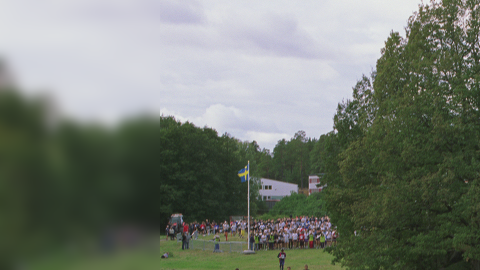
\includegraphics[width=6cm]{img/chap3/aboveMarathonFlou}};
	\draw (-1,1.7) -- (-1,-1.7);
	\node at (-2,1.2) {flou};
	\node at (4,0) {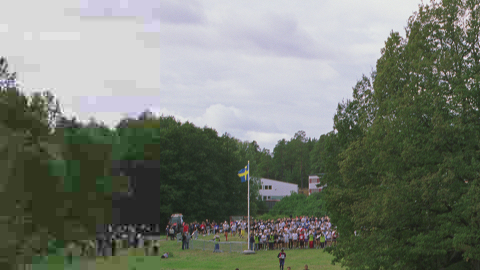
\includegraphics[width=6cm]{img/chap3/aboveMarathonBloc}};
	\draw (3,1.7) -- (3,-1.7);
	\node at (2,1.2) {effet de bloc};
	\node at (8,0) {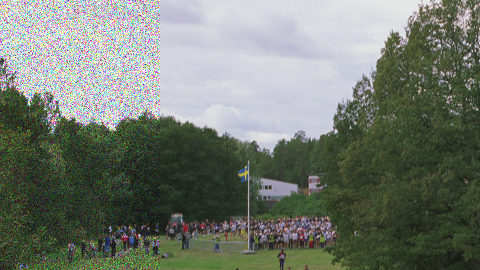
\includegraphics[width=6cm]{img/chap3/aboveMarathonBruit}};
	\draw (7,1.7) -- (7,-1.7);
	\node at (6,1.2) {bruit};
	\node at (2.5,-2) {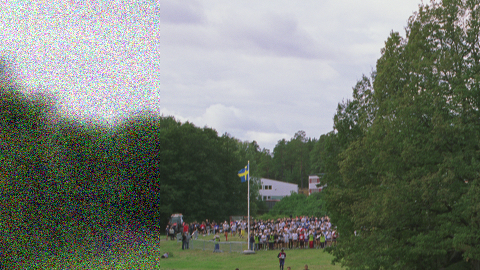
\includegraphics[width=6cm]{img/chap3/aboveMarathonFlouBruit.png}};
	\draw (1.5,-0.3) -- (1.5,-3.7);
	\node at (0.5,-0.8) {bruit+flou};
	\node at (5.5,-2) {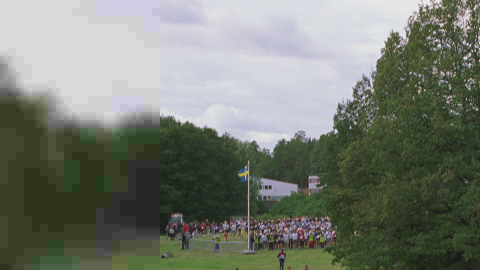
\includegraphics[width=6cm]{img/chap3/aboveMarathonBlocFlou.png}};
	\draw (4.5,-0.3) -- (4.5,-3.7);
	\node[text width=1.5cm] at (3.5,-0.8) {effet de bloc+flou};
	\node at (9,-2) {\dots};

	\node[action,text width=6cm] (node) at (0,-5.5) {tests de détection, description, mesure de gêne et d'intensité};
	\draw[fleche] (0,-4) -- (node);
	\draw[fleche] (node) -- (4,-5.5);

	\foreach \x in {4,4.5,5,5.5}
	{
			\draw[legende] (\x,-6.25) rectangle (\x + 1.5,-4.5);
			\draw[->] (\x + .25,-5.75) -- (\x + 1.25,-5.75);
			\draw[->] (\x + .25,-5.75) -- (\x + .25,-4.75) node[above=-0.1cm, font=\tiny] {gêne};
	}
	\node[below, font=\tiny] at (6.75,-5.75) {$I_{\mathit{flou}}$};
	\node[text width=5cm] at (5.5,-7) {une fonction de gêne par combinaison de dégradations};
	\draw[fleche] (7,-5.5) -- (8,-5.5);

	\draw[->] (8.5,-6.5) -- (10.5,-6.5) node[below] {$f(I_{\mathit{flou}}, \dots)$};
	\draw[->] (8.5,-6.5) -- (8.5,-4.5) node[right] {gêne};
% \end{tikzpicture}
	\end{tikzpicture}
	\caption{Schématisation de l'approche de Farias. $I_{\mathit{flou}}$ est un exemple de paramètre d'intensité d'une dégradation synthétique.}
	\label{fig:approcheFarias}
\end{figure}

L'inconvénient majeur de cette approche réside dans l'application arbitraire des dégradations à certaines zones spatiales de l'image. Or, lors de la construction de notre base de séquences présentée dans l'annexe~\ref{annex:base}, nous avons constaté la forte dépendance au contenu du procédé de codage. Nous considérons ainsi qu'une dégradation a une influence différente selon le domaine spatio-temporel où elle se situe. De plus, la campagne de test se révèle particulièrement complexe pour les observateurs car les dégradations synthétiques ne correspondent pas à des dégradations classiques de codage. L'impact mesuré est donc différent de celui recherché.

Une approche alternative a été proposée par Wolff~\cite{eusipco2006-wolff}. Elle consiste à considérer cette fois-ci des dégradations issues d'un système de codage \avc. L'évaluation subjective se fait toujours en utilisant une échelle différente pour chaque dégradation. Les observateurs ont deux tâches : évaluer la gêne globale sur la séquence et mesurer la force de chaque type de dégradation. Cette fois-ci en revanche, aucun contrôle de l'intensité des dégradations n'est possible. La critique principale de cette approche est liée à l'évaluation subjective qui demande aux observateurs d'isoler certaines dégradations, ce qui est une tâche complexe. Rien n'assure que le codage corresponde à une superposition des types de dégradations proposées. Encore une fois, l'approche est intéressante, mais la démarche risque de fournir des évaluations subjectives difficilement exploitables.


\subsection{Notre approche}
La gêne perçue par l'observateur dépend fortement du contexte local de chaque zone spatio-temporelle. Donc plutôt que de dégrader synthétiquement des zones choisies arbitrairement avec une ou plusieurs dégradations, notre approche consiste à dégrader des zones spatio-temporelles cohérentes avec un système de codage réel. La figure~\ref{fig:monApproche} schématise son fonctionnement. Nous substituons donc le partitionnement en dégradations par un partitionnement en zones spatio-temporelles cohérentes. Ainsi, notre objectif est de générer des séquences dégradées en fonction de ces zones et les évaluer subjectivement. Nous pourrons obtenir une fonction de gêne pour chaque zone spatio-temporelle. Une telle fonction représente la qualité subjective moyenne en fonction de l'intensité de la dégradation. Deux problèmes se posent alors. Le premier est le cumul des évaluations obtenues pour les zones. Afin d'obtenir une note de qualité globale sur la séquence, nous devons trouver une loi de combinaison adéquate. Le second problème concerne le contrôle de la quantité de dégradations injectées dans chaque zone. En effet, le débit seul n'est pas suffisant à représenter cette quantité. De plus, le partitionnement spatio-temporelle soulève des questions quand à la répartition et la visibilité des dégradations. Il nous faudra donc définir un paramètre de contrôle de la quantité de dégradations injectées dans les séquences dégradées.

\begin{figure}[htbp]
	\centering
	\begin{tikzpicture}[text centered]% \begin{tikzpicture}[text centered]
	\draw[legende] (-3.25,10) rectangle (3.25,-2.5);
	\node[text width=5cm] at (0,9.3) {\strong{création de séquences dégradées par classe de contenu}};
	\node at (0,7) {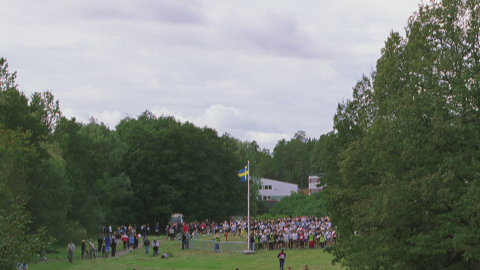
\includegraphics[width=6cm]{img/chap3/aboveMarathon}};
	\draw (-3,8) -- (-1.5,7.3) -- (1.1,7.3) -- (2.2,8.7);
	\node[legende,font=\small] at (-0.5,8) {zone uniforme};
	\node at (0,3.5) {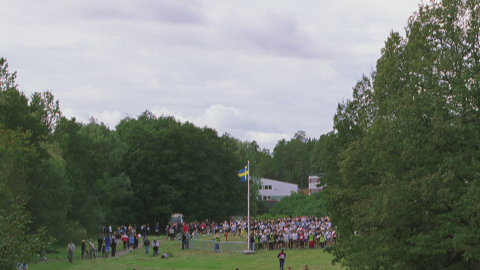
\includegraphics[width=6cm]{img/chap3/aboveMarathon}};
	\draw (-2.5,1.8) -- (-1.6,2.5) -- (1.2,2.5) -- (1.2,1.8);
	\node[legende,font=\small] at (-0.5,2.15) {textures fines};
	\node at (0,0) {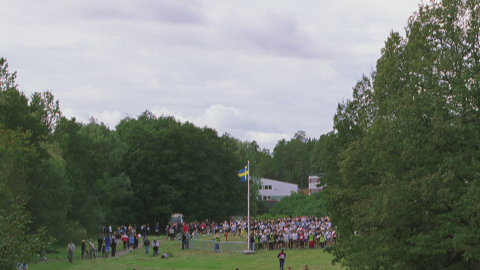
\includegraphics[width=6cm]{img/chap3/aboveMarathon}};
	\draw (-3,1) -- (-1.5,0.3) -- (1.1,0.3) -- (2.2,1.7);
	\draw (-2.5,-1.7) -- (-1.6,-1) -- (1.2,-1) -- (1.2,-1.7);
	\node[legende,font=\small] at (0,-0.5) {textures fortes et structurées};
	\node at (0,-2.1) {\dots};

	\node[action,text width=2cm] (node) at (6,7) {tests SAMVIQ};
	\draw[fleche] (3.25,7) -- (node);
	\draw[fleche] (node) -- (8,7);

	\foreach \x in {6.5,6,5.5,5}
	{
			\draw[legende] (8,\x) rectangle (9.5,\x + 1.5);
			\draw[->] (8.25,\x + .25) -- (8.25,\x + 1.25) node[above=-0.1cm, font=\tiny] {gêne};
			\draw[->] (8.25,\x + .25) -- (9.25,\x + .25);
	}
	\node[above] at (9.25,5.25) {?};
	\node[text width=3.5cm] at (6.25,5.5) {une fonction de gêne par classe de contenu};

	\draw[fleche] (8.75,5) -- (8.75,3.5);
	\node at (8,4.25) {cumul ?};
	\draw[->] (7.75,1) -- (9.75,1) node[below] {$D$};
	\draw[->] (7.75,1) -- (7.75,3) node[left] {gêne};
% \end{tikzpicture}
\end{tikzpicture}
	\caption{Schématisation de notre approche avec $D$ le débit utilisé pour dégrader la séquence d'origine. Les classes de contenu sont des approximations simplifiées pour la visualisation.}
	\label{fig:monApproche}
\end{figure}

Plusieurs bénéfices se dégagent a priori d'une telle approche. Tout d'abord, les défauts synthétiques introduits par Farias ne correspondent pas à la réalité du codage vidéo utilisé dans l'industrie. Notre approche est donc celle de Wolff qui utilise des dégradations réalistes liées à l'usage envisagé en production de télévision haute définition. Elles correspondent donc uniquement aux décisions prises par le codeur \avc{} lors de la quantification. De plus, l'aspect profondément temporel du processus d'évaluation de la qualité de la vidéo est trop souvent sous-estimé. Notre approche permet de tenir compte de cet aspect en évaluant notamment l'impact temporel des dégradations introduites. Ensuite, la gêne introduite par une dégradation dépend directement de son contexte local. Deux défauts de même intensité dont l'un est masqué par son contexte ne seront pas jugés de la même manière. Par exemple, appliquer une certaine erreur de quantification donne une dégradation particulièrement visible dans une zone homogène. Cependant, cette même erreur peut être partiellement ou totalement masquée dans une zone texturée. C'est pourquoi nous introduisons la notion de classification spatiale. %En considérant ensemble les aspects spatial et temporel, la classification nécessaire est spatio-temporelle.

L'étape préliminaire de notre méthode consiste à établir une typologie locale de la source vidéo. Ceci permet de définir l'ensemble de zones spatio-temporelles désiré. Les séquences suivent ensuite le schéma de la figure~\ref{fig:schemaGlobal}. Elles sont tout d'abord segmentées temporellement. Chaque segment est ensuite catégorisé suivant le partitionnement défini. Des séquences dégradées indépendamment par classe sont ensuite générées et évaluées. Ces évaluations fournissent des fonctions de gêne par type de zones. Cette gêne correspond à l'impact du système de codage sur chacune des partitions de l'espace spatio-temporelle de la séquence. Enfin, la question en suspend concerne la détermination d'un paramètre de contrôle de la quantité de dégradation injectée dans chaque zone. Nous en proposerons plusieurs modèles d'estimation.

\begin{figure}[htbp]
	\centering
	\begin{tikzpicture}[text centered, text width=2cm, node distance=2cm]% \begin{tikzpicture}[text centered, text width=2cm, node distance=2cm]
	\node[text width=1.5cm] (seq) {séquence};
	\node[action, right of=seq, node distance=2.5cm] (seg) {segmentation temporelle};
	\node[action, right of=seg, node distance=3cm] (classif) {classification};
	\node[action, below of=seq, node distance=2.6cm, text width=1.5cm] (codage) {codage H.264};
	\node[action, right of=codage, node distance=3cm, text width=2.5cm] (gene) {génération des séquences partiellement dégradées};
	\node[action, right of=gene, node distance=3cm] (eval) {évaluation subjective};
	\node[action, right of=eval, node distance=3cm, text width=2cm] (cumul) {cumul des évaluations locales};
	\node[right of=cumul, node distance=3cm, text width=1.5cm] (mos) {mesure globale de qualité};
	\draw[fleche] (seq) -- (seg);
	\draw[fleche] (seq) -- (codage);
	\draw[fleche] (seg) -- (classif);
	\draw[fleche] (codage) -- (gene);
	\draw[fleche] (classif) -- (gene) node[pos=0.5,right, text width=3cm] {séquences de classes};
	\draw[fleche] (gene) -- (eval);
	\draw[fleche] (eval) -- (cumul);
	\draw[fleche] (cumul) -- (mos);
% \end{tikzpicture}
\end{tikzpicture}
	\caption{Schéma global de la méthodologie proposée.}
	\label{fig:schemaGlobal}
\end{figure}


\section{Segmentation spatio-temporelle et classification du contenu d'une séquence vidéo} \label{sec:methodeClassifST}
Dans le but de mesurer l'impact de chaque zone spatio-temporelle, nous devons tout d'abord être en mesure de les dégrader indépendamment. C'est pourquoi une typologie du contenu local a été définie, conduisant à distinguer cinq classes de contenu local. Ensuite, la segmentation spatio-temporelle ne peut être réaliser en même dans le temps et dans l'espace. Nous devons donc séparer le problème en deux phases comme le montre la figure~\ref{fig:segmentationClassification}. Tout d'abord, un suivi temporel est réalisé localement grâce à une estimation de mouvement. Puis, chaque volume élémentaire élémentaire est labellisé suivant son contenu. Nous réalisons ces deux phases sur des contenus non dégradés de résolution 1920\texttimes1080 en mode entrelacé.

\begin{figure}[htbp]
	\centering
	\begin{tikzpicture}[text centered, text width=2cm, node distance=4.5cm]
		\node[text width=1.5cm] (seq) {séquence};
		\node[action, right of=seq, node distance=3cm] (seg) {segmentation temporelle};
		\node[action, right of=seg] (classif) {classification de chaque segment};
		\node[right of=classif, node distance=4cm, text width=3cm] (out) {séquence segmentée avec chaque segment classifié};

		\draw[fleche] (seq) -- (seg);
		\draw[fleche] (seg) -- (classif) node[above, pos=0.5] {segments};
		\draw[fleche] (classif) -- (out);
	\end{tikzpicture}
	\caption{Découpement de la méthodologie en deux phases successives.}
	\label{fig:segmentationClassification}
\end{figure}


\subsection{Définition des classes de contenu local} \label{ssec:classes_De_Contenu}
Nous proposons une typologie du contenu local d'une source vidéo en adéquation avec les considérations spatio-temporelles que nous avons énoncées. La catégorisation qui découle de cette typologie correspond à une segmentation spatio-temporelle du flux vidéo. Nous considérons le signal d'image $I$ comme la somme d'une composante structurelle $I_S$ et une composante texturelle $I_T$ auxquelles s'ajoute une composante éventuelle de bruit $I_B$ : $I = I_S + I_T + I_B$. La composante structurelle correspond à la valeur moyenne locale et aux transitions brusques de valeur moyenne sur les contours de l'image. La composante texturelle correspond aux variations du signal d'image autour de sa valeur moyenne locale. Plusieurs zones sont alors définies, en fonction du comportement de ces composantes. Notons que la composante de bruit $I_B$, bien que peu considérée ici, peut s'avérer particulièrement visible en TVHD. Ceci s'explique à la fois par les médiocres performances des appareils de capture et par l'amplification du rendu de ce défaut par les écrans de technologie LCD.

Quatre types de zones sont ainsi définies. Il s'agit des zones uniformes, des zones de textures fines, des zones de textures fortes et des zones de contours. Nous en déduisons cinq classes de contenu local en distinguant les zones uniformes de faible et de forte luminance.


\subsubsection{Zones uniformes}
Les zones uniformes correspondent à une évolution soit constante, soit très régulière et faible du signal d'image, où les textures sont très fines, constituées de hautes fréquences spatiales. Ici, $I_T$ et $I_B$ sont proches de zéro et $I_S$ ne contient pas de contours, donc $I \simeq I_S$.

Les défauts générés dans ces zones sont généralement des pertes des détails fins, laissant apparaitre des plaques, apparentées à de l'effet de bloc. Le rendu est simplifié par le codage \avc{} en annulant les faibles contrastes de texture. Ceci est dû à la décomposition en DCT \emph{(Discrete Cosine Transform)} entière  des blocs 16\texttimes16 de l'image. Les composantes continues de ces blocs sont regroupées dans un bloc 4\texttimes4 qui est à son tour codé par une transformation de Hadamard. La quantification a ensuite lieu dans cet espace transformé, ce qui explique la perte des hautes fréquences.

Le mouvement ajoute à ces zones l'effet dit de « vitre sale ». La structure de codage en bloc est visible et ne bouge pas, alors que les objets de la scène sont en mouvement. La cohérence temporelle n'est pas respectée, à cause des changements de stratégie de codage prise par le codeur au cours du temps.


\subsubsection{Zones de textures fines}
Il s'agit par exemple de la texture d'une chevelure ou d'un terrain de sport comme le football. Ces textures sont plutôt aléatoires et de moyennes fréquences spatiales. $I_S$ ne contient pas de contours et $I_T$ est de dynamique pas très importante. $I_B$ est de dynamique faible ou nulle. %Dans ce cas, le signal d'image est de la forme $I = I_S + I_T + I_B$.

Le faible nombre de niveaux de quantification utilisés pour le codage de ces zones simplifie le rendu des textures, ce qui entraine un phénomène de rendu en plaques. Celui-ci correspond à la succession temporelle de modifications de la structure des textures. La structure passe d'une composition assez complète à une version simplifiée ne contenant plus les détails et vice versa, ce qui est particulièrement gênant pour le spectateur.


\subsubsection{Zones de textures fortes et structurées}
Dans ces zones, la composante structurelle ne contient pas de rupture. La composante texturelle est de dynamique moyenne à forte pouvant être la somme d'une texture structurée et d'une texture fine. Les défauts visibles dans ces zones sont des irrégularités constatées dans le rendu des structures. L'effet vient de l'interaction de la position de ces structures et de la structure d'échantillonnage. Ces structures ont un meilleur contraste quand elles sont placées entre deux pixels que lorsqu'elles tombent sur un pixel, comme le montre la figure~\ref{fig:zone3}. Le rendu varie le long du déplacement de la structure, ce qui peut entrainer jusqu'à son déchiquetage. La perception du mouvement manque alors de cohérence.

\begin{figure}[htbp]
	\centering
	\begin{tikzpicture}[text centered]% \begin{tikzpicture}[text centered]
\foreach \i in {0,1,2,3,4} {
	\foreach \j in {0,1,2,3,4,5,6,7,8,9} {
		\draw[help lines] (\j,\i-0.1) -- (\j,\i+0.1);
		\draw[help lines] (\j-0.1,\i) -- (\j+0.1,\i);
	};
};
\draw[thick] (0.5,-0.5) -- (1.2,0) -- (1.7,1.5) -- (2.2,1.5) -- (2.4,2) -- (3.9,2.8) -- (4.1,3.4) -- (5.4,4.5);
\draw[thick] (2.9,-0.5) -- (3.6,0) -- (4.1,1.5) -- (4.6,1.5) -- (4.8,2) -- (6.3,2.8) -- (6.5,3.4) -- (7.6,4.5);

\fill[fill=white] (-1,2.5) rectangle (2.5,4.5);

\path[fleche] (1,4.5) -- (4,4.5) node[above,pos=0.5] {mouvement};

\path[fleche] (1,3.5) -- (3.8,3.1);
\path[fleche] (1,3.5) -- (4.7,2.1);

\path[fleche] (6.5,-0.2) -- (6.5,2.8);
\path[fleche] (6.5,-0.2) -- (2.6,1.9);

\node at (6.5,-0.5) {contraste fort};
\node[text width=2cm] at (0,3.5) {contraste faible};
% \end{tikzpicture}
\end{tikzpicture}
	\caption{Schéma montrant l'interaction de la position de la structure de texture et de la structure d'échantillonnage.}
	\label{fig:zone3}
\end{figure}


\subsubsection{Zones de contours}
Dans ces zones, la composante structurelle contient un ou plusieurs contours. De plus,$I_T$ est de dynamique inférieure à celle de $I_S$, soit $I_T \ll I_S$.

Les défauts présents dans ces zones sont similaires à ceux présents dans les zones à textures structurées. Cependant, ils sont amplifiés puisque le contraste y est encore plus important. En mouvement perpendiculaire au contour, la structure d'erreur est d'autant plus visible que le contraste est fort.


\subsubsection{Classes de contenu}
À partir de cette définition de la source vidéo en type de zones, nous définissons des classes de contenu local. Celles-ci correspondent en grande partie aux zones, à une exception près. En effet, nous avons montré que l'un des principaux défaut des écrans LCD était leur difficulté à rendre les zones de faible luminance. Or l'\oe il humain distingue bien les faibles variations de luminance dans ces zones sombres. Dans le but de les étudier en particulier, nous avons décidé de créer deux classes distinctes pour les zones uniformes selon qu'elles sont à luminance plutôt faible ou plutôt forte.

Nous sommes désormais en mesure d'identifier les cinq classes de contenu local que nous allons utiliser. Il s'agit des classes :
\begin{itemize}
\item $C_1$ pour les zones uniformes de luminance faible ;
\item $C_2$ pour les zones uniformes de luminance moyenne et forte ;
\item $C_3$ pour les zones de textures fines ;
\item $C_4$ pour les zones de textures moyennes et fortes ;
\item $C_5$ pour les zones de contours.
\end{itemize}


\subsection{Segmentation temporelle}
L'étape de segmentation consiste à créer des volumes spatio-temporels élémentaires le long du mouvement local. La détermination de la durée adaptée découle de la manière dont l'\oe il fixe une scène. Notre vision est une succession de saccades et de fixations. Les saccades sont des mouvement rapides permettant de déplacer le regard d'un point de fixation à l'autre. Les fixations, moments où le regard reste stationnaire, correspondent donc à la vision utile. La durée d'une fixation est l'intervalle entre deux saccades soit environ 200 ms en moyenne. Cette durée moyenne varie d'un individu à l'autre et en fonction de la tâche à accomplir. C'est pourquoi nous considérons des ensembles de cinq images consécutives, correspondant donc à une durée moyenne de fixation. Un tel groupe de cinq images est appelé un « tronçon ».

Le principe de construction des volumes élémentaires est de suivre temporellement chaque bloc de l'image centrale sur les quatre autres images du tronçon. Cet ensemble de cinq blocs forme ce que nous appelons un « tube » spatio-temporel élémentaire. Une estimation de mouvement permet ainsi de suivre l'évolution de chaque bloc au cours du temps. Ce concept de tubes tridimensionnels a été introduit par Wolf et Pinson~\cite{wolf-spatempmetric}. Dans leurs travaux, les tubes sont toujours orientés suivant la direction du temps, alors que dans notre approche, ils sont orientés chacun dans la direction locale du mouvement. Cela les rend plus cohérents en termes d'activités spatiale et temporelle.

Le traitement débute par séparer la vidéo source entrelacée en deux trames. Chaque trame est découpée en blocs de taille 16\texttimes8 qui correspondent à des blocs 16\texttimes16 pour les images entrelacées. Il y a donc 8040 blocs 16\texttimes16 dans une image 1920\texttimes1080 dont nous ne considérons pas les huit dernières lignes. Pour chaque groupe de cinq trames, la trame centrale est le centre de l'estimation de mouvement calculée pour chaque bloc. Elle utilise les deux trames de même parité suivantes et les deux précédentes comme le montre la figure~\ref{fig:tubeDansImage}.

\begin{figure}[htbp]
	\centering
	\begin{tikzpicture}[scale=0.5]
		% schéma du tube dans une image

% \begin{tikzpicture}[scale=0.5]

% zones de recherche
\filldraw[fill=blue!20, dashed] (0,-6) -- (4.5,-3.75) -- (4.5,3.5) -- (0,1.25) node[below right=-2pt, rotate=26.2]{\iflanguage{french}{zone de recherche}{research area}} -- cycle;
\fill[fill=blue!20] (6,-0.25) -- (8.5,1) --  (8.5,-2.75) -- (6,-4) -- cycle;
\fill[fill=blue!20] (16,-4) -- (18.5,-2.75) --  (18.5,1) -- (16,-0.25) -- cycle;
\fill[fill=blue!20] (20,-6) -- (24.5,-3.75) --  (24.5,3) -- (20,0.75) -- cycle;

% blocs rouges
\filldraw[fill=red!40] (0.6,-1) -- (1.1,-0.75) --  (1.1,0) -- (0.6,-0.25) -- cycle;
\filldraw[fill=red!40] (6.3,-0.75) -- (6.8,-0.5) --  (6.8,-1.25) -- (6.3,-1.5) -- cycle;
\filldraw[fill=red!40] (12,-1.25) -- (12.5,-1) --  (12.5,-1.75) -- (12,-2) -- cycle;
\filldraw[fill=red!40] (17.7,-1.75) -- (18.2,-1.5) --  (18.2,-2.25) -- (17.7,-2.5) -- cycle;
\filldraw[fill=red!40] (23.4,-3) -- (23.9,-2.75) --  (23.9,-2) -- (23.4,-2.25) -- cycle;

% lignes reliant les blocs rouges
\draw[help lines, dashed] (0.6,-0.25) -- (12,-1.25) -- (23.4,-2.25);
\draw[help lines, dashed] (1.1,0) -- (12.5,-1) -- (23.9,-2);
\draw[help lines, dashed] (0.6,-1) -- (12,-2) -- (23.4,-3);
\draw[help lines, dashed] (1.1,-0.75) -- (12.5,-1.75) -- (23.9,-2.75);

\foreach \i in {0.25,0.5,0.75,1,1.25,1.5,1.75} % grille sur l'image centrale
{
	\draw (10+2*\i,\i) -- (10+2*\i,-6+\i);
	\draw (10,-3*\i) -- (14,2-3*\i);

	\foreach \j in {0,1,3,4} % grille sur les autres images
	{
		\draw[help lines] (5*\j + 2*\i, \i) -- (5*\j + 2*\i, -6 + \i);
		\draw[help lines] (5*\j,-3*\i) -- (5*\j + 4,2-3*\i);
	}
}

\draw[dashed] (6,-0.25) -- (8.5,1) --  (8.5,-2.75) -- (6,-4) -- cycle;
\draw[dashed] (16,-4) -- (18.5,-2.75) --  (18.5,1) -- (16,-0.25) -- cycle;
\draw[dashed] (20,-6) -- (24.5,-3.75) --  (24.5,3) -- (20,0.75) -- cycle;
\draw[dashed] (0,-6) -- (4.5,-3.75) -- (4.5,3.5) -- (0,1.25) -- cycle;
\draw (2,-8) node{$i-2$};
\draw (7,-8) node{$i-1$};
\draw (12,-8) node{trame $i$};
\draw (17,-8) node{$i+1$};
\draw (22,-8) node{$i+2$};


% \end{tikzpicture}


	\end{tikzpicture}
	\caption{Schéma de l'estimation de mouvement d'un bloc.}
  \label{fig:tubeDansImage}
\end{figure}

Tous les vecteurs de mouvement inclus dans la zone de recherche sont évalués. La taille de cette zone de recherche est choisie de telle sorte que le mouvement le plus rapide de la séquence y soit contenu. Le vecteur de mouvement retenu est celui qui minimise l'erreur quadratique moyenne entre le bloc de la trame centrale et les blocs des quatre autres trames. Ce calcul est effectué sur les trois composantes YCbCr des blocs. Enfin, le vecteur de mouvement d'un bloc 16\texttimes16 est pris comme la moyenne des deux vecteurs des blocs 16\texttimes8 pair et impair correspondants.

Devant la complexité et le temps de calcul d'un tel traitement sur des séquences de TVHD, l'estimation de mouvement est effectuée sur une représentation multi-résolution de chaque trame. Elle est d'abord calculée sur la plus basse résolution. Puis, le vecteur de mouvement obtenu est ajusté en prenant compte de la résolution supérieure, et ainsi de suite. Trois niveaux hiérarchiques ont ainsi permis de réduire significativement le temps de calcul.


\subsection{Classification des tubes}
Une fois la segmentation temporelle terminée, nous avons à disposition un ensemble de tubes spatio-temporels orientés suivant le mouvement local. Nous devons maintenant leur assigner une classe à chacun. %, tout en assurant la cohérence temporelle du contenu.
La classification d'un tube est déduite de ses caractéristiques d'activité. Ces caractéristiques permettent d'assigner une classe à chaque tube.


\subsubsection{Caractéristiques d'activité d'un tube}
Elles sont basées sur la quantité de gradient horizontaux et verticaux contenus dans chaque tube. Pour un pixel $p(m,n,r)$ d'un tube, la composante horizontale $\Delta H$ et la composante verticale $\Delta V$ du gradient spatial sont calculées par :
\begin{equation}
\Delta H(m,n,r) = | p(m, n+1,r) - p(m,n,r)| \ \text{et}\ \Delta V(m,n,r) = | p(m+1, n,r) - p(m,n,r)|
\end{equation}
%
dont nous calculons les sommes $\overline{\Delta H}$ et $\overline{\Delta V}$ sur le tube $t$ :
%
\begin{equation}
\overline{\Delta H} = \sum_{\substack{1\le m\le 16 \\ 1\le n\le 16 \\ 1\le r \le 5}} \Delta H(m,n,r) \quad \text{et}\quad \overline{\Delta V} = \sum_{\substack{1\le m\le 16 \\ 1\le n\le 16 \\ 1\le r \le 5}} \Delta V(m,n,r).
\end{equation}

Ainsi, chaque tube peut être localisé dans un espace $\Psi=(\overline{\Delta H}, \overline{\Delta V})$ que nous partitionnons suivant nos classes de contenu. La figure~\ref{fig:deltaHdeltaV} présente la structure d'un tel espace. Ainsi, un tube dont les caractéristiques se situent dans la région étiquetée ($C_1\bigcup C_2$) appartient à une zone homogène. Si elles se situent dans $C_3$ ou $C_4$, alors il appartient respectivement à une zone de textures fines ou de contours. Enfin, $C_5$ est la région indéterminée. Elle contient les tubes pour lesquels nous ne pouvons lever l'ambiguïté concernant l'orientation spatiale. Pour ces tubes, nous calculons les composantes du gradient suivant les deux directions diagonales, à 45° et 135°  :
\begin{equation}
\Delta D_{45}(m,n,r) = | p(m+1, n-1,r) - p(m,n,r)| \ \text{et}\ \Delta D_{135}(m,n,r) = | p(m+1, n+1,r) - p(m,n,r)|
\end{equation}
%
dont nous calculons également les sommes $\overline{\Delta D_{45}}$ et $\overline{\Delta D_{135}}$ sur le tube $t$ :
\begin{equation}
\overline{\Delta D_{45}} = \sum_{\substack{1\le m\le 16 \\ 1\le n\le 16 \\ 1\le r \le 5}} \Delta D_{45}(m,n,r) \qquad \text{et}\qquad \overline{\Delta D_{135}} = \sum_{\substack{1\le m\le 16 \\ 1\le n\le 16 \\ 1\le r \le 5}} \Delta D_{135}(m,n,r).
\end{equation}

\begin{figure}[htbp]
	\centering
	\subfloat[\label{fig:deltaHdeltaV}Espace $\Psi=(\overline{\Delta H}, \overline{\Delta V})$ des gradients horizontal et vertical.]{\begin{tikzpicture}[scale=3.2]% \begin{tikzpicture}[scale=3.2]

\clip (-0.15,-0.15) rectangle (2,2);
\fill[fill=black!20] (0,0) -- (22:1.6cm) arc (22:68:1.6cm) node[below right=20pt,text width=1cm,text centered] {?};

\fill[fill=green!20] (0,0) -- (0:1.1) arc (0:90:1.1);
\draw[thick] (1.1,0) arc (0:90:1.1);

\fill[fill=blue!20] (0,0) -- (68:1.6cm) arc (68:90:1.6cm) node[below right=5pt,text width=1cm,text centered] {$C_4$};
\fill[fill=blue!20] (0,0) -- (0:1.6cm) arc (0:22:1.6cm)  node[below=20pt,text width=2cm,text centered] {$C_4$};
\draw[thick] (0,0) -- (68:1.8cm);
\draw[thick] (0,0) -- (22:1.8cm);

\fill[fill=green!20] (0,0) -- (0:0.8) arc (0:90:0.8);
\draw (0.7,0.7) node {$C_3$};
\draw[thick] (0.8,0) arc (0:22:0.8);
\draw[thick] (0,0.8) arc (90:68:0.8);

\fill[fill=yellow!20] (0,0) -- (0:0.6) arc (0:90:0.6);
\draw (0.35,0.25) node[text width=2cm] {($C_1\bigcup C_2$)};
\draw[thick] (0.6,0) arc (0:90:0.6);

\draw[thick, ->] (-1.7,0) -- (1.7,0) node[right] {$\overline{\Delta H}$};
\draw[thick, ->] (0,-1.7) -- (0,1.7) node[above] {$\overline{\Delta V}$};

\draw[thin, <->] (0.9,0) arc (0:22:0.9) node[below right] {$A_1$};
\draw[thin, <->] (1.3,0) arc (0:68:1.3);
\draw (1.15,0.8) node {$A_2$};

% \end{tikzpicture}\end{tikzpicture}}\hfill
	\subfloat[\label{fig:deltaD}Espace $\Psi'=(\overline{\Delta D_{45}}, \overline{\Delta D_{135}})$ des gradients diagonaux.]{\begin{tikzpicture}[scale=3.2]\clip (-0.15,-0.15) rectangle (2,2);

\fill[fill=black!20] (0,0) -- (22:1.6) arc (22:68:1.6) node[below right=20pt,text width=1cm,text centered] {$C'_5$};

\fill[fill=green!20] (0,0) -- (0:1.1) arc (0:90:1.1);
\draw[thick] (1.1,0) arc (0:90:1.1);

\fill[fill=blue!20] (0,0) -- (68:1.6) arc (68:90:1.6) node[below right=5pt,text width=1cm,text centered] {$C'_4$};
\fill[fill=blue!20] (0,0) -- (0:1.6) arc (0:22:1.6)  node[below=20pt,text width=2cm,text centered] {$C'_4$};
\draw[thick] (0,0) -- (68:1.8);
\draw[thick] (0,0) -- (22:1.8);

\fill[fill=green!20] (0,0) -- (0:0.8) arc (0:90:0.8);
\draw (0.7,0.7) node {$C'_3$};
\draw[thick] (0.8,0) arc (0:22:0.8);
\draw[thick] (0,0.8) arc (90:68:0.8);

\fill[fill=yellow!20] (0,0) -- (0:0.6) arc (0:90:0.6);
\draw (0.35,0.25) node[text width=2cm] {($C'_1\bigcup C'_2$)};
\draw[thick] (0.6,0) arc (0:90:0.6);

\draw[thick, ->] (-1.7,0) -- (1.7,0) node[right] {$\overline{\Delta D_{45}}$};
\draw[thick, ->] (0,-1.7) -- (0,1.7) node[above] {$\overline{\Delta D_{135}}$};

\draw (0.6,-0.08) node{$Y_1$};
\draw (0.8,-0.08) node{$Y_2$};
\draw (1.1,-0.08) node{$Y_3$};
\end{tikzpicture}}\\
	\caption{Espaces permettant la classification des blocs.}
\end{figure}

Comme précédemment, chaque tube est localisé dans un espace $\Psi'=(\overline{\Delta D_{45}}, \overline{\Delta D_{135}})$, formé de manière identique à $\Psi$ et présenté sur la figure~\ref{fig:deltaD}. Dans ce nouveau plan, un tube dont les caractéristiques se situent dans la région étiquetée ($C'_1\bigcup C'_2$) appartient à une zone homogène. Si elles se situent dans $C'_3$ ou $C'_4$, alors il appartient respectivement à une zone de textures fines ou de contours. Si elles sont dans $C'_5$, le tube appartient à une zone de textures fortes.

Enfin, la distinction entre les tubes des classes $C_1$ et $C_2$ correspondant respectivement aux zones uniformes de luminance faible et aux zones uniformes de luminance moyenne et forte se fait à l'aide d'un seuil. Nous considérons qu'une zone est de faible luminance si sa luminance moyenne est inférieure à un cinquième de la dynamique environ. C'est pourquoi, si le tube a un niveau de gris moyen sur l'ensemble de ces pixels inférieur à 50 sur l'échelle $[\text{0};\text{255}]$, il est assigné à la classe $C_1$. Sinon, il appartient à la classe $C_2$. La classification se termine une fois chaque tube de la séquence classé. Les objets en mouvement le long de la séquence entière sont ainsi suivis. Les tubes voisins et appartenant à la même classe se regroupent naturellement en un volume spatio-temporel de cette classe.


\subsubsection{Assurer une cohérence temporelle}
Si la classification d'un tube était uniquement assurée par le calcul des gradients, des discontinuités importantes pourraient apparaitre. Afin d'obtenir une classification cohérente d'un tronçon à l'autre, un suivi des tubes de proche en proche est réalisé. Pour cela, les tubes spatio-temporels qui se suivent temporellement sont assemblés afin de constituer des régions spatio-temporelles sur la séquence entière. Ceci est illustré par la figure~\ref{fig:overlapTubes}. Cet assemblage consiste à regrouper un tube d'un tronçon avec le tronçon suivant pour faire correspondre des tubes qui se suivent temporellement. Cela permet de prolonger les tubes d'un tronçon à l'autre en cumulant les gradients sur une durée supérieure à un tube. La classification se fait alors sur cet ensemble de tubes, assurant une cohérence temporelle.

\begin{figure}[htbp]
	\centering
	\begin{tikzpicture}[scale=1.5]
		% \begin{tikzpicture}[scale=2.5]

% jointure derrière les tubes
\draw(0.9,-0.8)--(3.9,-0.4);
\draw(4.3,-0.3)--(7.6,0.5);
\draw[dashed](4.3,-0.3)--(3.9,-0.4);

% blocs rouges
\filldraw[fill=red!40] (0.7,-0.7) -- (0.9,-0.5) --  (0.9,-0.8) -- (0.7,-1) -- cycle;
\filldraw[fill=red!40] (1.45,-0.6) -- (1.65,-0.4) --  (1.65,-0.7) -- (1.45,-0.9) -- cycle;
\filldraw[fill=red!40] (2.2,-0.5) -- (2.4,-0.3) --  (2.4,-0.6) -- (2.2,-0.8) -- cycle;
\filldraw[fill=red!40] (2.95,-0.4) -- (3.15,-0.2) --  (3.15,-0.5) -- (2.95,-0.7) -- cycle;
\filldraw[fill=red!40] (3.7,-0.3) -- (3.9,-0.1) --  (3.9,-0.4) -- (3.7,-0.6) -- cycle;

% blocs bleus
\filldraw[fill=blue!40] (4.1,-0.2) -- (4.3,0) --  (4.3,-0.3) -- (4.1,-0.5) -- cycle;
\filldraw[fill=blue!40] (4.925,0) -- (5.125,0.2) --  (5.125,-0.1) -- (4.925,-0.3) -- cycle;
\filldraw[fill=blue!40] (5.75,0.2) -- (5.95,0.4) --  (5.95,0.1) -- (5.75,-0.1) -- cycle;
\filldraw[fill=blue!40] (6.575,0.4) -- (6.775,0.6) --  (6.775,0.3) -- (6.575,0.1) -- cycle;
\filldraw[fill=blue!40] (7.4,0.6) -- (7.6,0.8) --  (7.6,0.5) -- (7.4,0.3) -- cycle;

% jointure inter-tube
\draw[dashed](4.1,-0.2)--(3.7,-0.3);
\draw[dashed](4.3,0)--(3.9,-0.1);
\draw[dashed](4.1,-0.5)--(3.7,-0.6);

% images
\foreach \j in {0,1,2,3,4,5,6,7,8,9} % grille sur les autres images
{
	\draw[help lines](0.75*\j,0)--(1 + 0.75*\j,1)--(1+0.75*\j,-1)--(0.75*\j,-2)--cycle;
}

% tubes
\draw(0.7,-0.7)--(3.7,-0.3);
\draw(0.7,-1)--(3.7,-0.6);
\draw(0.9,-0.5)--(3.9,-0.1);
\draw(4.1,-0.2)--(7.4,0.6);
\draw(4.3,0)--(7.6,0.8);
\draw(4.1,-0.5)--(7.4,0.3);

% labels
\path (0,-2.2) node {$i-2$}  -- (0.75,-2.2) node {$i-1$} -- (1.5,-2.2) node {$i$} -- (2.25,-2.2) node {$i+1$} -- (3,-2.2) node {$i+2$} -- (3.75,-2.2) node {$i+3$} -- (4.5,-2.2) node {$i+4$} -- (5.25,-2.2) node {$i+5$} -- (6,-2.2) node {$i+6$} -- (6.75,-2.2) node {$i+7$};
\path (1.5,1.5);


% \end{tikzpicture}
	\end{tikzpicture}
	\caption{Schéma de la fusion des tubes se chevauchant.}
  \label{fig:overlapTubes}
\end{figure}


\subsubsection{Paramétrage de la création du partitionnement des espaces \texorpdfstring{$\Psi$}{Psi} et \texorpdfstring{$\Psi'$}{Psi'}} \label{ssec:paramClass}
Les paramètres permettant de modifier la classification sont les angles et les rayons délimitant les régions des espaces $\Psi$ et $\Psi'$. Le rayon de la région $C_1$ est nommé $Y_1$, le premier de la région $C_3$ est nommé $Y_2$ et le second $Y_3$. L'angle le plus petit est nommé $A_1$, alors que le plus grand est nommé $A_2$. Réduire ou augmenter les valeurs de ces paramètres influent sur les tailles des régions spatio-temporelles et donc sur l'appartenance d'un tube à telle ou telle classe.

Diverses combinaisons de paramètres ont été testées, indépendamment pour chaque contenu. Un ensemble de paramètre pertinent permet de bien distinguer les zones spatio-temporelles principales de la séquence. Une telle vérification peut se faire visuellement. Ainsi, les paramètres ont été déterminées de manière à obtenir une classification aussi réaliste que possible.


\subsection{Conclusion}
Dans cette section, nous avons présenté la méthode de segmentation spatio-temporelle et de classification utile à notre étude. Cette méthode est effectuée en deux phases. La première consiste à segmenter temporellement des séquences en tubes élémentaires. Ceux-ci ont la particularité de suivre le mouvement local et ainsi de conserver un contenu cohérent. La seconde phase classe chaque tube suivant l'activité spatiale de son contenu. La cohérence temporelle est assurée par un suivi de proche en proche des tubes.


\section{Mise en \oe uvre de la méthodologie}
Afin de tester la méthodologie proposée, nous avons utilisé les douze contenus de l'ensemble SVT2006 décrits dans la section~\ref{ssec:seq-svt2006} et les séquences dégradées par le codage \avc{} correspondantes. À partir de ces données, nous avons généré des séquences partiellement dégradées. Le tableau~\ref{tab:paramClasses} donne les valeurs des paramètres de la création des régions pour chaque contenu. Ces paramètres ont été déterminés après visualisation des séquences. Plusieurs étapes sont requises pour générer les séquences finales comme le montre la figure~\ref{fig:miseEnOeuvre}. La première de ces étapes est la génération d'une séquence vidéo contenant en chaque pixel une représentation de la classe du pixel correspondant dans la séquence d'origine. Cette séquence est utilisée pour substituer les pixels dégradés aux pixels originaux. Des traitements sont utilisés pour assurer la segmentation totale de la séquence et pour adoucir la visibilité des transitions.

\begin{figure}[htbp]
	\centering
	\begin{tikzpicture}[scale=1.5, text width=2.5cm, node distance=3.2cm, text centered]
		\node[text width=1.4cm] (seq) {tubes classifiés};
		\node[action, right of=seq, node distance=3cm] (seg) {génération des séquences de classes};
		\node[action, right of=seg] (comp) {complétion de la segmentation};
		\node[action, right of=comp] (gene) {génération des séquences partiellement dégradées};
		\node[right of=gene, text width=2cm] (out) {séquences partiellement dégradées};
		\draw[fleche] (seq) -- (seg);
		\draw[fleche] (seg) -- (comp);
		\draw[fleche] (comp) -- (gene);
		\draw[fleche] (gene) -- (out);
	\end{tikzpicture}
	\caption{Étapes de la génération des séquences partiellement dégradées.}
  \label{fig:miseEnOeuvre}
\end{figure}

\begin{table}[htbp]
\centering
\begin{tabular}{cccccc}\toprule
\strong{contenu}					& $A_1$ & $A_2$ & $Y_1$ & $Y_2$ & $Y_3$ \\ \toprule
\emph{Above Marathon}			& 20 & 70 & 8 & 10 & 13\\ \midrule
\emph{Captain}						& 20 & 70 & 8 & 10 & 13\\ \midrule
\emph{Dance in the Woods}	& 20 & 70 & 8 & 10 & 13\\ \midrule
\emph{Duck Fly}						& 10 & 80 & 8 & 10 & 13\\ \midrule
\emph{Fountain Man}				& 25 & 65 & 8 & 10 & 13\\ \midrule
\emph{Group Disorder}			& 20 & 70 & 10 & 15 & 20\\ \midrule
\emph{Inside Marathon}			& 20 & 70 & 10 & 15 & 20\\ \midrule
\emph{New Parkrun}				& 20 & 70 & 8 & 10 & 13\\ \midrule
\emph{Rendezvous}				& 20 & 70 & 8 & 10 & 13\\ \midrule
\emph{Stockholm Travel}		& 25 & 65 & 8 & 10 & 13\\ \midrule
\emph{Tree Pan}						& 20 & 70 & 8 & 10 & 13\\ \midrule
\emph{Ulriksdals}					& 20 & 70 & 8 & 10 & 13\\ \bottomrule
\end{tabular}
\caption{Valeurs des paramètres de création des régions pour chaque contenu.}
\label{tab:paramClasses}
\end{table}


\subsection{Résultats de la classification}
Le procédé de classification fournit les classes de chaque tube. Chaque classe représente une certaine proportion du contenu total. Ces proportions sont présentées dans le tableau~\ref{tab:proportionsClasses}. Nous remarquons que la classe $C_1$ couvre une gamme de proportions allant de pratiquement zéro (0,13\%) à 42\%. La classe $C_2$ couvre la plus large gamme de valeurs. Les vidéos contenant de l'eau qui tombent comme \emph{Captain} ou \emph{Fountain Man} ont une proportion particulièrement élevée de zones de type $C_2$ avec plus de 78\%. Ceci est dû à la classification dans $C_2$ des zones de chute d'eau. Les classes $C_3$ et $C_4$ ont une forte importance, entre 6\% et 54\% pour la première et entre 0.36\% à plus de 60\% pour la dernière. Enfin, la classe $C_5$ a une importance particulièrement faible, en dessous de 3\% sauf pour deux vidéos. Ces proportions sont consistantes avec la nature du contenu. Ceux-ci sont réalistes avec des scènes en extérieur. Ainsi, nous y trouvons peu de contours, quelques zones homogènes comme le ciel ou les vêtements et beaucoup de textures comme les arbres et l'herbe.

\begin{table}[htbp]
\centering
\begin{tabular}{cccccc} \toprule
\strong{contenu}					& $C_1$ & $C_2$ & $C_3$ & $C_4$ & $C_5$ \\ \toprule
\emph{Above Marathon}			& 3,75 & 17,45 & 27,79 & 50,06 & 0,94\\\midrule
\emph{Captain}						& 13,14 & 78,26 & 6,81 & 0,36 & 1,43 \\\midrule
\emph{Dance in the Woods}	& 3,80 & 22,57 & 53,86 & 16,75 & 3,02 \\\midrule
\emph{Duck Fly}						& 0,13 & 8,97 & 19,50 & 60,70 & 10,70\\\midrule
\emph{Fountain Man}				& 10,52 & 70,71 & 13,37 & 3,94 & 1,46 \\\midrule
\emph{Group Disorder}			& 25,28 & 38,59 & 29,80 & 4,54 & 1,79\\\midrule
\emph{Inside Marathon}			& 5,64 & 47,64 & 39,77 & 6,75 & 0,20 \\\midrule
\emph{New Parkrun}				& 41,89 & 32,98 & 17,67 & 3,49 & 3,97 \\\midrule
\emph{Rendezvous}				& 8,78 & 12,38 & 19,87 & 56,91 & 2,05 \\\midrule
\emph{Stockholm Travel}		& 8,02 & 58,63 & 14,23 & 1,53 & 17,59\\\midrule
\emph{Tree Pan}						& 1,96 & 16,63 & 22,58 & 58,15 & 0,68 \\\midrule
\emph{Ulriksdals}					& 13,54 & 41,31& 40,48 & 3,31 & 1,36 \\\bottomrule
\end{tabular}
\caption{Proportions des classes de chaque contenu exprimées en pourcentage.}
\label{tab:proportionsClasses}
\end{table}


\subsection{Création de masques de classes}
À partir des classes des tubes d'une séquence, une séquence de classes est générée. Il s'agit d'assigner une valeur particulière de luminance à chaque pixel appartenant à une classe donnée. Ceci permet de repérer visuellement les zones spatio-temporelles. La figure~\ref{fig:videoClasse} présente un exemple de classification obtenue par notre méthode. Bien sûr, elle ne rend pas compte de l'aspect temporel de celle-ci.

\begin{figure}[htbp]
	\centering
	
\includegraphics[width=0.98\linewidth]{img/chap3/videoClasseMobcalOrdered}
	\begin{tikzpicture}
		\draw[legende] (-2.5,-4.4) rectangle (2.5,-5);
		\node at (0,-4.7) {
\includegraphics[scale=7]{img/chap3/legendClasse1} $C_1$ 
\includegraphics[scale=7]{img/chap3/legendClasse2} $C_2$ 
\includegraphics[scale=7]{img/chap3/legendClasse3} $C_3$ 
\includegraphics[scale=7]{img/chap3/legendClasse4} $C_4$ 
\includegraphics[scale=7]{img/chap3/legendClasse5} $C_5$};
	\end{tikzpicture}
	\caption{Image de la séquence des classes du contenu New Mobile \& Calendar.}
	\label{fig:videoClasse}
\end{figure}

Tous les pixels de l'image centrale d'un tronçon sont assignés à une classe. Cependant, la méthode de création des tubes laisse des pixels sans classification sur les autres images. Parallèlement, elle provoque aussi le recouvrement partiel de tubes à d'autres endroits. La segmentation n'est donc pas complète. Afin de créer des séquences dont tous les pixels sont étiquetés, nous leur assignons tous une classe en affectant à un pixel non étiqueté la classe du tube le plus proche spatialement. La même méthode est utilisée pour déterminer la classe d'un pixel où se recouvre plusieurs tubes. La figure~\ref{fig:avecTrous} présente un exemple de vidéos de classe avant ce traitement. La figure~\ref{fig:sansTrous} présente ce même exemple après ce traitement. Ainsi, chaque pixel du contenu traité appartient à une unique classe.

\begin{figure}[htbp]
	\centering
	\subfloat[\label{fig:avecTrous}Avant traitement.]{
\includegraphics{img/chap3/avantRemplissageTrousOrdered}}\hfill
	\subfloat[\label{fig:sansTrous}Après traitement.]{
\includegraphics{img/chap3/apresRemplissageTrousOrdered}}\\
	\begin{tikzpicture}
		\draw[legende] (-3.5,-4.4) rectangle (3.5,-5);
		\node at (0,-4.7) {
\includegraphics[scale=7]{img/chap3/legendTrou} sans étiquette 
\includegraphics[scale=7]{img/chap3/legendClasse1} $C_1$ 
\includegraphics[scale=7]{img/chap3/legendClasse2} $C_2$ 
\includegraphics[scale=7]{img/chap3/legendClasse3} $C_3$ 
\includegraphics[scale=7]{img/chap3/legendClasse4} $C_4$ 
\includegraphics[scale=7]{img/chap3/legendClasse5} $C_5$};
	\end{tikzpicture}
	\caption{Comparaison de deux vidéos de classe, la première avant suppression des zones sans classes et des ambiguïtés de classification, la seconde après.}
\end{figure}


\subsection{Génération des séquences partiellement dégradées}
Les séquences partiellement dégradées sont générées à partir du contenu original, de sa segmentation et classification et des séquences codées à différents débits par \avc{} correspondantes. Les segments d'une séquence dégradée correspondant à une classe sont insérées dans le contenu original. Ce procédé crée une séquence dégradée par classe et par débit. Seuls les segments de la séquence d'une classe donnée sont ainsi dégradés, les autres segments étant ceux de la vidéo d'origine. Les étapes sont présentées sur la figure~\ref{fig:etapesSeqPartDeg} avec seulement le quart de la première image du contenu \emph{Above Marathon}. L'image~\ref{fig:aM-2M-C1} représente les différents segments avec leur classe. L'image~\ref{fig:aM-MC} montre l'image dégradée partiellement : seuls les segments de classe $C_1$ sont dégradés. Ceci est visible sur l'arbre central. Nous créons ainsi cinq séquences partiellement dégradées par contenu et par débit. Pour cette étude, vingt débits ont été sélectionnés par des experts. Ils sont donnés dans le tableau~\ref{tab:debitsClasses}. Par ailleurs, les bordures entre une zone dégradée et une zone d'origine pouvant être visibles, nous les avons adoucies à l'aide d'une fonction d'apodisation d'extension spatiale d'une dizaine de pixels.

\begin{figure}[htbp]
	\centering
	\subfloat[\label{fig:aM}Image du contenu original.]{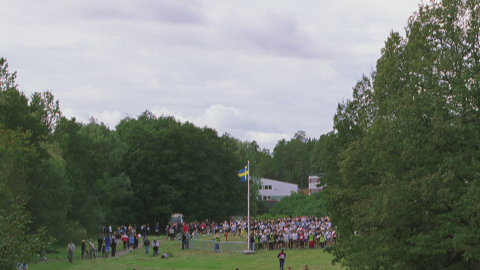
\includegraphics[scale=0.56]{img/chap3/aboveMarathon}}\\
	\subfloat[\label{fig:aM-2M-C1}Image de la vidéo de classes.]{
\includegraphics[scale=0.56]{img/chap3/aboveMarathonMetaClassesOrdered}}\\
	\begin{tikzpicture}
		\draw[legende] (-2.5,0.3) rectangle (2.5,-0.3);
		\node {
\includegraphics[scale=7]{img/chap3/legendClasse1} $C_1$ 
\includegraphics[scale=7]{img/chap3/legendClasse2} $C_2$ 
\includegraphics[scale=7]{img/chap3/legendClasse3} $C_3$ 
\includegraphics[scale=7]{img/chap3/legendClasse4} $C_4$ 
\includegraphics[scale=7]{img/chap3/legendClasse5} $C_5$};
	\end{tikzpicture}\\
	\subfloat[\label{fig:aM-MC}Image de la séquence partiellement dégradée. Les segments de la classe $C_1$ sont ici seuls dégradés.]{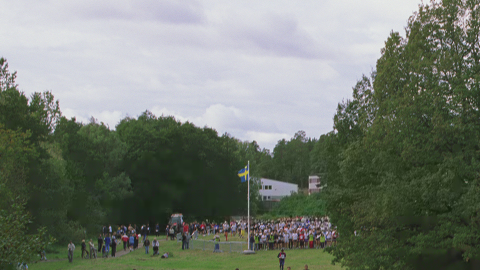
\includegraphics[scale=0.56]{img/chap3/aboveMarathon-2M-class1}}\\
	\caption{Les trois étapes de création des séquences partiellement dégradées.}
	\label{fig:etapesSeqPartDeg}
\end{figure}


\begin{table}[htbp]
\centering
\begin{tabular}{cc}\toprule
\textbf{contenu}						& \textbf{débits (Mbps)} \\ \toprule
\emph{Above Marathon}			& 5 ; 8 ; 10	\\\midrule
\emph{Captain	}						& 1 ; 3 ; 5		\\\midrule
\emph{Dance in the Woods}	& 3 ; 5 ; 6		\\\midrule
\emph{Duck Fly}						& 4 ; 6 ; 8		\\\midrule
\emph{Fountain Man}				& 1 ; 5			\\\midrule
\emph{Group Disorder}			& 2 ; 4			\\\midrule
\emph{Rendezvous}				& 6 ; 8			\\\midrule
\emph{Ulriksdals}					& 1 ; 4			\\\bottomrule
\end{tabular}
\caption{Débits en Mbps utilisés pour la création de séquences partiellement dégradées.}
\label{tab:debitsClasses}
\end{table}


\subsection{Évaluation subjective de la qualité des séquences dégradées}
Afin de disposer des notes de qualité de chacune des séquences partiellement dégradées, nous effectuons une campagne de tests. La mesure obtenue est liée à l'impact d'une classe donnée sur la qualité perçue pour le niveau de dégradation créé par le codage au débit considéré. Les tests ont été réalisés dans les mêmes conditions que pour l'évaluation de la qualité visuelle des vidéos de la base de l'annexe~\ref{annex:base}. Une session SAMVIQ pour un contenu donné et à un débit $B$ est composée :

\begin{enumerate}
\item du contenu de référence explicite, servant d'ancre de haute qualité ;
\item de la séquence partiellement dégradée par la classe $C_1$, codé au débit $B$ ;
\item de la séquence partiellement dégradée par la classe $C_2$, codé au débit $B$ ;
\item de la séquence partiellement dégradée par la classe $C_3$, codé au débit $B$ ;
\item de la séquence partiellement dégradée par la classe $C_4$, codé au débit $B$ ;
\item de la séquence partiellement dégradée par la classe $C_5$, codé au débit $B$ ;
\item de la séquence entièrement dégradée, par le codage au débit $B$ ;
\item d'une séquence entièrement dégradée à bas débit, servant d'ancre de basse qualité ;
\item d'une séquence entièrement dégradée à un débit moyen, choisi selon $B$ et le bas débit ;
\item de la référence cachée.
\end{enumerate}

Une session permet donc de recueillir à la fois les notes de qualités de chaque séquence entièrement dégradée et celles de toutes les séquences partiellement dégradées.


\subsection{Conclusion}
Nous avons présenté la méthode de segmentation spatio-temporelle et de classification de séquences vidéo que nous avons conçue afin de mesurer l'impact des dégradations dans chaque type de segment spatio-temporel. Cela nous a permis de connaitre les pertes de qualité liées à chaque classe séparément. Nous avons également mesuré les pertes de qualité quand l'ensemble de la séquence est dégradé. Celles-ci sont issues des tests de qualité de la base de l'annexe~\ref{annex:base}. Il ne reste désormais plus qu'à tenter de relier les impacts visuels des dégradations locales à celle des dégradations globales.


\section{De la perte de qualité subjective locale à l'estimation globale} \label{sec:deLocalAGlobal}
Nous cherchons à savoir s'il est possible de relier les pertes de qualité locales d'un côté et la perte de qualité globale de l'autre. Il n'est pas évident a priori qu'une telle relation soit simple, étant donné que le cumul correspondant est fait au niveau du cerveau humain au cours de l'évaluation subjective de qualité. Si nous pouvons identifier cette relation, cela sera très intéressant pour construire un modèle objectif de qualité. En effet, celui-ci pourrait alors évaluer séparément chaque classe de contenu avant de cumuler les qualités locales en une note de qualité globale.

Commençons par clarifier les termes utilisés. La note de qualité visuelle du contenu $S_j$ non dégradé est notée MOS$(S_j)$. Dans la méthodologie SAMVIQ, elle correspond à la note de la référence cachée. La note de la séquence entièrement dégradée à un débit $B_k$ correspondante est notée MOS$(S_j,B_k)$. De plus, une note de qualité partielle, notée MOS($S_j, B_k, C_i$), est obtenue pour chaque contenu $S_j$, codé au débit $B_k$ et avec une dégradation présente uniquement sur les segments de classe $C_i$. La différence entre MOS$(S_j)$ et MOS$(S_j,B_k)$ représente la perte de qualité globale de la séquence. Nous la notons DMOS$(S_j,B_k)$. La différence entre une note de qualité partielle MOS($S_j, B_k, C_i$) et la note de qualité MOS$(S_j)$ est appelée $\Delta$MOS($C_i, S_j, B_k$). Elle indique la perte de qualité induite par les dégradations de la classe $C_i$. Pour un contenu $S_j$ et un débit $B_k$ donnés, la relation recherchée est donc entre DMOS$(S_j,B_k)$ et les cinq valeurs $\Delta$MOS($C_i, S_j, B_k$) avec $i\in [\text{1};\text{5}]$. La figure~\ref{fig:DMOSDeltaMOS} représente les différentes valeurs présentes dans ce type de relation. Sur une échelle de qualité allant de 0 à 100, la valeur MOS$(S_j)$ est la note maximale obtenue et MOS$(S_j,B_k)$ la note minimale. Les $\Delta$MOS($C_i, S_j, B_k$) sont donc compris entre ces deux extrêmes.

Plusieurs modèles de cumul ont été testés dans le but d'établir la relation cherchée. Nous présentons ici les plus intéressants. Nous distinguerons deux catégories : les modèles linéaires et les non linéaires.

\begin{figure}[htbp]
	\centering
	\begin{tikzpicture}[yscale=1.5]% échelle
\draw[->,-latex,very thick] node[left=72pt] {0} (-3,0) -- node[anchor=west,pos=1] {100} (-3,10);

% ref et deg
\draw[thick,dashed] (-3,9) -- (2.5,9) node[right]{MOS$(S_j)$};
\draw[thick,dashed] (-3,2) -- (2.5,2) node[right]{MOS$(S_j,B_k)$};

% DMOS
\draw[<->,latex-latex,thick] (-4,2) -- node[left]{DMOS$(S_j,B_k)$} (-4,9);

% DeltaMOS des classes
\draw[<->,latex-latex,thick] (-2,5) 	-- node[above,pos=0,rotate=90]	{$\Delta$MOS$(S_j,C_1,B_k)$} (-2,9);
\draw[<->,latex-latex,thick] (-1,4) 	-- node[above,pos=0,rotate=90]	{$\Delta$MOS$(S_j,C_2,B_k)$} (-1,9);
\draw[<->,latex-latex,thick] (0,6) 	-- node[above,pos=0,rotate=90]	{$\Delta$MOS$(S_j,C_3,B_k)$} (0,9);
\draw[<->,latex-latex,thick] (1,7) 	-- node[above,pos=0,rotate=90]	{$\Delta$MOS$(S_j,C_4,B_k)$} (1,9);
\draw[<->,latex-latex,thick] (2,3) 	-- node[above,pos=0,rotate=90]	{$\Delta$MOS$(S_j,C_5,B_k)$} (2,9);

\end{tikzpicture}
	\caption{Représentation des différentes valeurs présentes dans la relation entre la perte de qualité globale, notée DMOS$(S_j,B_k)$, et les pertes locales notées $\Delta$MOS($C_i, S_j, B_k$) avec $i\in [\text{1};\text{5}]$.}
	\label{fig:DMOSDeltaMOS}
\end{figure}


\subsection{Modèles linéaires} \label{ssec:modeleLin}
Ces modèles, les plus simples consistent à calculer le DMOS du contenu $S_j$ au débit $B_k$ par :
\begin{equation}
\text{DMOS}(S_j,B_k) = \sum_{\substack{1\le i \le 5}}\Delta\text{MOS}(C_i, S_j, B_k) \times \delta_i
\end{equation}
%
avec $\delta_i$ valant 0 ou 1. Ainsi, soit la contribution d'une classe est prise en compte entièrement, soit elle ne l'est pas du tout. En effet, ceci nous renseignera sur l'importance relative de chaque classe sur le cumul. Il y a ainsi 31 modèles différents possibles. Nous évaluons les performances de chacun d'eux par deux critères : le coefficient de corrélation linéaire et l'écart-type de la différence, noté $\sigma_e$. Cet écart-type est calculé entre les $\Delta$MOS$_i$ et leurs prédictions linéaires $\Delta$MOSp$_i$ issues d'un modèle donné $X$. La prédiction consiste à calculer  :
\begin{equation}
\Delta\text{MOSp}_i = \left(\rho_{X\Delta} \times \left(\frac{X_i - \overline{X}}{\sigma_X}\right) \times \sigma_\Delta \right) + \overline{\Delta}
\end{equation}
%
avec $\rho_{X\Delta}$ le coefficient de corrélation entre les notes $X_i$ issues du modèle $X$ et les $\Delta$MOS$_i$, $\overline{X}$ la moyenne des $X_i$, $\sigma_X$ l'écart-type des $X_i$, $\overline{\Delta}$ la moyenne des $\Delta$MOS$_i$ et $\sigma_\Delta$ l'écart-type des $\Delta$MOS$_i$.

Le tableau~\ref{tab:combination} présente certains des modèles proposés avec le coefficient de corrélation et la racine carrée de l'erreur quadratique moyenne qu'ils donnent. Pour les modèles dont le coefficient de corrélation est inférieur à 0,9, seuls ceux issus de l'utilisation d'une seule classe sont présentés. Le nom de chaque modèle est symbolisé par la somme des classes prises en compte dans celui-ci.

\begin{table}[htbp]
\centering
\begin{tabular}{ccc}\toprule
\textbf{modèle}					& \textbf{coefficient de corrélation}		& $\sigma_e$ \\ \toprule
$C_2+C_4+C_5$					& 0,9485			& 4,11			\\\midrule
$C_2+C_4$							& 0,9440			& 4,28			\\\midrule
$C_2+C_3+C_5$					& 0,9094			& 5,40			\\\midrule
$C_1+C_2+C_3+C_4+C_5$	& 0,9058			& 5,50			\\\midrule
$C_1+C_2+C_4+C_5$			& 0,9052			& 5,52			\\\midrule
$C_2+C_3+C_4+C_5$			& 0,9041			& 5,55			\\\midrule
$\cdots$								& $\cdots$		& $\cdots$	\\\midrule
% $C_2+C_3$						& 0,8978			& \\\midrule
% $C_1+C_2+C_4$				& 0,8939			& \\\midrule
% $C_1+C_2+C_3+C_4$		& 0,8936			& \\\midrule
% $C_2+C_3+C_4$				& 0,8892			& \\\midrule
% $C_1+C_4+C_5$				& 0,8739			& \\\midrule
% $C_1+C_2+C_3+C_5$		& 0,8447			& \\\midrule
% $C_1+C_3+C_4+C_5$		& 0,8442			& \\\midrule
% $C_1+C_4$						& 0,8379			& \\\midrule
% $C_1+C_2+C_3$				& 0,8291			& \\\midrule
% $C_1+C_3+C_4$				& 0,8183			& \\\midrule
% $C_1+C_3+C_5$				& 0,7995			& \\\midrule
% $C_2+C_5$						& 0,7765			& \\\midrule
$C_2$									& 0,7664			& 8,33			\\\midrule
% $C_1+C_3$						& 0,7635			& \\\midrule
% $C_3+C_4+C_5$				& 0,7515			& \\\midrule
% $C_3+C_5$						& 0,7154			& \\\midrule
% $C_4+C_4$						& 0,7154			& \\\midrule
% $C_3+C_4$						& 0,7130			& \\\midrule
$C_3$									& 0,7094			& 9,15			\\\midrule
% $C_1+C_2+C_5$				& 0,7073			& \\\midrule
% $C_1+C_2$						& 0,6810			& \\\midrule
$C_4$									& 0,6400			& 9,97			\\\midrule
% $C_1+C_5$						& 0,6102			& \\\midrule
$C_5$									& 0,5472			& 10,86		\\\midrule
$C_1$									& 0,5349			& 10,96		\\\bottomrule
\end{tabular}
\caption{Modèles linéaires de cumul des pertes de qualité locales accompagnés de leur performances respectives.}
\label{tab:combination}
\end{table}

Les performances révèlent l'importance relative de chaque classe dans le processus de cumul effectué par l'observateur moyen. Malgré sa simplicité, une telle approche permet de bonnes corrélations avec quelques classes stratégiques. La combinaison des seules zones homogènes de forte luminance $C_2$ et des zones de textures fortes $C_4$ fournit une très bonne corrélation avec le jugement humain. Ceci s'explique notamment par la nature des contenus, composés en majorité de ce type de zones. Malgré ses faibles proportions et ses mauvaises performances individuelles, la classe des contours $C_5$ est présente dans cinq des six premiers modèles les plus performants. Ainsi, l'ensemble des dégradations de ces trois classes $C_2$, $C_4$ et $C_5$ sont étroitement liées à la qualité globale de la séquence. Leur impact sur la perception de la qualité par l'observateur moyen est donc particulièrement important.

À l'opposé, lorsqu'une seule classe est utilisée, nous obtenons parmi les plus mauvaises performances. Cela signifie que la qualité d'une seule classe de contenu ne suffit pas à représenter la qualité globale de la séquence, ce qui semble évident a priori. En contrepartie, la combinaison des cinq classes n'obtient pas la meilleure performance, indiquant que certaines zones ne sont pas ou peu prises en compte dans la construction du jugement de qualité de l'observateur moyen. Cela pourrait être affiné avec des valeurs non entières de $\delta$.

Un modèle linéaire simple peut donc suffire à fournir une très bonne corrélation entre la qualité globale et les qualités locales. Ce résultat est très intéressant car il montre que les qualités locales peuvent être cumulées afin d'approcher la qualité globale. Ainsi, nous pouvons passer de l'évaluation de la séquence entière à une évaluation par parties, chacune exploitant la classe de contenu où elle est calculée.


\subsection{Modèles non linéaires}
Des modèles non linéaires peuvent également être envisagés. Le premier que nous proposons est également très simple et ne considère que les valeurs maximales des $\Delta$MOS. Le second est plus évolué et introduit la notion d'unités de dégradation.


\subsubsection{Modèle basé sur les valeurs maximales des pertes locales}
Ce modèle considère que les classes avec la plus grande perte locale contribuent le plus à la perte globale. Il s'exprime par :
\begin{equation}
\text{DMOS}(S_j,B_k) = \max_i \left(\Delta\text{MOS}(C_i, S_j, B_k)\right)
\end{equation}
%
Ainsi, en ne retenant que la classe de plus grand $\Delta$MOS pour chaque contenu, le coefficient de corrélation linéaire vaut 0,9467 et la racine carrée de l'erreur quadratique moyenne vaut 4,179. Si la somme des deux classes qui contribuent le plus est utilisée, c'est-à-dire :
\begin{equation}
\text{DMOS}(S_j,B_k) = \max_i \left(\Delta\text{MOS}(C_i, S_j, B_k)\right) + \max_{l, l\neq i} \left(\Delta\text{MOS}(C_l, S_j, B_k)\right)
\end{equation}
%
alors le coefficient de corrélation linéaire vaut 0,9530 et la racine carrée de l'erreur quadratique moyenne vaut 3,933. Les classes retenues sont majoritairement les classes $C_2$ et $C_3$, ce qui confirme leur importance.

Le modèle utilisant les deux classes de plus forte contribution obtient de meilleures performances que tous les modèles linéaires présentés précédemment. L'idée de résumer la perte à ses plus grands contributeurs est donc bonne. Cependant, l'inconvénient majeur de cette méthode est qu'elle nécessite la connaissance a priori de toutes les notes de qualités locales afin de pouvoir en sélectionner les valeurs maximales.


\subsubsection{Modèle de prédiction des qualités basé sur l'unité de dégradation}
Ce modèle ne prédit pas les pertes de qualité locales, mais directement les notes de qualité, c'est-à-dire les MOS. Il exploite pour cela la notion d'unité de dégradation~\cite{ccir}. La définition de l'unité de dégradation $U_{\mathit{ijk}}$ associée à la qualité $Q_{\mathit{ijk}} =$ MOS($C_i, S_j, B_k$) de la classe $C_i$ du contenu $S_j$ au débit $B_k$ est :
\begin{equation}
U_{\mathit{ijk}} = \frac{\hat{Q}_{j} - Q_{\mathit{ijk}}}{Q_{\mathit{ijk}}} = \frac{\hat{Q}_{j}}{Q_{\mathit{ijk}}} - 1
\end{equation}
avec $\hat{Q}_{j} = 100$ la qualité de référence. En effet, nous considérons ici que la qualité de référence doit être optimale, c'est-à-dire que la prise de vue est parfaite. Or dans nos tests, le MOS $Q_{j}$ de la référence cachée est la plus haute valeur et ne vaut jamais 100. C'est pourquoi dans ce modèle, nous appliquons une pondération $w_j$ à chaque MOS du contenu $S_j$ afin de transformer la valeur de la référence cachée pour qu'elle vaille 100 :
\begin{equation}
Q_{\mathit{ijk}}' = w_j \times Q_{\mathit{ijk}} = \frac{100}{Q_{j}}\times Q_{\mathit{ijk}}.
\end{equation}
Un modèle de cumul des unités de dégradation de chaque classe $C_i$ est définie par :
\begin{equation}
U_{jk} = \sum_{i=1}^5 U_{\mathit{ijk}} = \frac{\hat{Q}_{j}}{Q_{\mathit{jk}}} - 1
\end{equation}
et la prédiction de la note de qualité globale du contenu $S_j$ au débit $B_k$ est donc :
\begin{equation}
Q_{\mathit{jk}} = \frac{\hat{Q}_{j}}{1+U_{\mathit{jk}}}.
\end{equation}

Nous utilisons ce modèle pour prédire les MOS des 20 séquences du tableau~\ref{tab:debitsClasses}. Le coefficient de corrélation linéaire entre les MOS subjectifs et les MOS prédits vaut 0,9160. La racine carrée de l'erreur quadratique moyenne vaut 5,934. En considérant uniquement les trois classes les plus significatives, à savoir $C_2$, $C_4$ et $C_5$, le coefficient de corrélation augmente à 0,9583 et l'erreur chute à 4,226. Encore une fois, ne considérer que les classes les plus importantes améliore significativement les performances. Ce modèle obtient ainsi la meilleure corrélation pour une erreur légèrement supérieure à celle des meilleurs modèles linéaires et des modèles basé sur les valeurs maximales des pertes locales.


\subsection{Conclusion}
Nous venons de présenter plusieurs modèles de cumul des pertes de qualités locales en une évaluation de la perte globale de qualité. Seul le dernier est une prédiction directe des notes de qualité. Les meilleurs modèles obtiennent une très bonne corrélation entre les données subjectives et leur prédiction. Le tableau~\ref{tab:MeilleuresCombinaisons} récapitule les meilleures performances de chaque modèle. Le principal enseignement de cette étude est qu'il est possible de trouver une relation entre des évaluations de qualité partielles et l'évaluation de la séquence complète. De plus, les modèles proposés sont tous simples d'utilisation, ce qui renforce leur intérêt.

\begin{table}[htbp]
\centering
\begin{tabular}{ccc}\toprule
\textbf{modèle}							& \textbf{coefficient de corrélation}	& \textbf{reqm}	\\ \toprule
linéaire											& 0,9485												& 4,11\\ \midrule
non linéaire									& 0,9530												& 3,933\\ \midrule
prédiction des notes de qualité 	& 0,9583 												& 4,226\\ \bottomrule
\end{tabular}
\caption{Meilleures performances des modèles de cumul des pertes de qualité locales.}
\label{tab:MeilleuresCombinaisons}
\end{table}


\section{Conclusion}
Ce chapitre a permis de présenter et d'exploiter une méthodologie originale. Son but est de permettre la caractérisation de l'impact d'un système dégradant de type codage sur la qualité visuelle. Dans le cadre de la télévision haute définition, le système de codage retenu suit la norme \avc. Notre approche prolonge les travaux de Farias~\cite{farias-phd} mais nous remplaçons son partitionnement en type de dégradations par un partitionnement en zones spatio-temporelles cohérentes. L'idée étant posée, il fallait ensuite construire une méthode permettant de l'exploiter. Nous avons donc proposé une segmentation spatio-temporelle qui introduit notamment la notion de tubes 3D dont l'originalité est de suivre le mouvement local. Cette segmentation permet de dégrader un contenu par zones spatio-temporelles suivant leur activité spatiale. Chaque zone est ensuite évaluée individuellement, ce qui permet de recueillir les qualités locales de chaque séquence. Ainsi, l'analyse de l'impact du codage sur la qualité visuelle est plus fine. Néanmoins, la méthode est indépendante du système dégradant, elle pourrait être utilisée dans d'autres contextes.

La question à laquelle nous avons ensuite répondu est celle du cumul de ces notes de qualité par type de contenu en une note de qualité globale. Nous avons montré que de simples combinaisons linéaires entre les pertes de qualité par type de contenu et la perte globale de qualité permettaient d'obtenir une relation forte. Ainsi, l'impact sur la qualité globale peut être déduite des impacts sur chaque type de contenu local.


%Ce résultat est très intéressant car il ouvre la voie à un modèle objectif évaluant la quantité de dégradation globale à partir des dégradations locales. %Dans un second temps, nous avons proposé une fonction de gêne pour l'une des zones spatio-temporelles définies. Pour cela, nous avons contruit plusieurs paramètres de contrôle de la quantité de dégradations d'une même zone spatio-temporelle, répondant ainsi à la problématique de l'injection de dégradation dans une classe.


\ornementChapitre

% \chapter*{Bilan des tests subjectifs réalisés} \addcontentsline{toc}{chapter}{Bilan des tests subjectifs réalisés} % TODO à vérifier
Cette première partie a abordé la question de la qualité visuelle en télévision haute définition d'un point de vue subjectif. Nous l'avons vu, cet aspect nécessite de lourdes expérimentations. À titre informatif, voici quelques chiffres caractérisant, chacun à leur façon, l'ensemble des tests que nous avons réalisés. Nous avons utilisé :
\begin{itemize}
\item une salle de test dédiée et normalisée selon les recommandations internationales~\cite{itu-bt500-11,itu-bt710-4} ;
\item une chaine complète de lecture de séquences de télévision haute définition non compressées comprenant deux écrans haute définition, un lecteur temps-réel et un serveur de stockage ;
\item près de deux téraoctets de séquences vidéos ;
\item plus de 750 jours cumulés de codage H.264 avec le codeur de référence~\cite{h264-jm} ;
\item une interface de notation pour chacune des trois méthodologies utilisées ;
\item 20 sessions SAMVIQ, 4 sessions ACR et 2 sessions de préférence ;
\item 600 séances de test pour environ 300 heures d'évaluation subjective de la qualité ;
\item une base de plus de 200 observateurs uniques, dont l'acuité est vérifiée par le test de Monoyer~\cite{monoyer-plates} et l'absence de daltonisme par les tests d'Ishihara~\cite{ishihara-plates}.
\end{itemize}

Les deux écrans de résolution 1920\texttimes1080 utilisés étaient un CRT JVC DT-V 1910CG et un LCD Philips T370HW01. Le premier, de type CRT, a une hauteur d'image de 20,5 cm, ce qui donne une distance d'observation de 61,5 cm en se plaçant à trois fois la hauteur de l'écran. Le second écran est un LCD de 46 cm de hauteur, correspondant à une distance d'observation normalisée de 138 cm. Le lecteur temps-réel de contenu haute définition 1080i non compressé était un système Dorémi V1-UHD.


% photo ?

%
% %%% partie 2 - Partie « objective »
% \part[Critères objectifs de qualité vidéo \texorpdfstring{\\}{}en télévision haute définition]{Critères objectifs de qualité vidéo \\en télévision haute définition}
% %%%%%%%%%%%%%%%%%%%%%%%%%%%%%%%%%%%%%%%%%%%%%%%%%
%%%
%%% Auteur : Stéphane Péchard - stephane.pechard@univ-nantes.fr
%%% Fichier : 4-metriques.tex - chapitre 4 :  Critères objectifs de qualité vidéo et création d'une base de séquences (30 pages)
%%% Version : 0.1
%%% Date : 2007/09/10
%%%
%%%%%%%%%%%%%%%%%%%%%%%%%%%%%%%%%%%%%%%%%%%%%%%%%
\chapter{Critères objectifs de qualité vidéo : état de l'art} \label{chap:criteres}
\opt{final}{\lettrine[lines=4]{L}{a littérature propose}}\opt{nofinal}{La littérature propose} de nombreuses méthodes d'évaluation objective de la qualité de la vidéo. Ce chapitre a pour objectif de présenter de façon structurée une vue d'ensemble des principales approches existantes. Nous la limitons sciemment au domaine applicatif qui nous concerne : le codage. Pourtant, les applications de l'évaluation objective de la qualité vidéo sont plus diverses. La transmission, les post-traitements, les capteurs ou les afficheurs sont également des éléments pouvant faire l'objet de critères de qualité spécifiques. Les critères objectifs de qualité vidéo sont de trois types différents, suivant la disponibilité ou non du signal vidéo d'origine, dit de référence, car supposé non dégradé. Pour le premier type, appelé avec référence complète (noté FR pour \emph{Full Reference}), les méthodes disposent de la vidéo de référence en plus de la vidéo dont la qualité est à mesurer. Ceci est le cas ici car le codage s'effectue à partir de la vidéo de référence et la version dégradée est la vidéo après codage/décodage. La plupart des méthodes proposées dans la littérature fonctionnent de cette manière et c'est ce type que nous traiterons ici en grande majorité. Nous ne considérerons pas le cas du transcodage. Le second type de méthodes, appelées avec référence réduite (RR pour \emph{Reduced Reference}), produit une mesure de qualité en ne disposant que d'un ensemble réduit de caractéristiques mesurées sur la référence. Les mêmes caractéristiques calculées sur la vidéo dégradée leur sont comparées afin de construire la note de qualité finale. Le peu d'information disponible pour la conception rend celle-ci plus difficile que pour les méthodes avec référence complète. Par contre, ce type de méthode s'applique très bien à la transmission de la vidéo car la référence réduite est codée avec une quantité d'informations binaires très réduite par rapport à celle utilisée dans le codage du contenu. Enfin, les méthodes sans référence (notées NR pour \emph{No Reference}) calculent un critère sans aucune connaissance du signal d'origine. Alors que l'\oe il humain est le plus souvent capable d'évaluer une qualité d'image sans connaitre la référence associée, la conception d'un critère de qualité visuelle sans référence est une tâche particulièrement complexe. C'est pourquoi peu de critères de ce type ont été proposés dans la littérature jusqu'à présent. Cependant, pour améliorer les performances des méthodes avec référence réduite ou sans références, il est possible de s'appuyer des a priori sur le système dégradant utilisé.

Nous utiliserons en plus ici une classification de plus haut niveau que celle distinguant les niveaux de disponibilité de la référence. Celle que nous adoptons distingue les approches n'exploitant pas les propriétés du système visuel humain de celles qui en exploitent. Les premières tiennent uniquement compte des données brutes de la vidéo. Les secondes intègrent des principes de plus ou moins haut niveau du système visuel humain. Ceci leur permet de rendre compte de l'impact des données sur la perception de la qualité. Dans cette catégorie d'approche, plusieurs courants co-existent. La figure~\ref{fig:vueGlobale} tente de représenter l'ensemble des approches abordées dans ce chapitre, avec des exemples de critères pour chacune d'elle. Ces critères seront mentionnés et détaillés dans la suite de ce chapitre.

\begin{figure}[htbp]
  \centering
  \begin{tikzpicture}[text centered,scale=1.04]% \begin{tikzpicture}[text centered]

% ellipses bleues
\filldraw[thick,dashed,fill=blue!20] (1.5,0.1) ellipse (3cm and 1.2cm);
\filldraw[thick,dashed,fill=blue!20] (-0.5,-1.75) ellipse (2cm and 0.7cm);
\filldraw[thick,dashed,fill=blue!20] (1,-3.5) ellipse (3cm and 1cm);
\filldraw[thick,dashed,fill=blue!20] (6.5,-1.5) ellipse (2.5cm and 2cm);

% ellipses
\draw (-2,-1.5) ellipse (3cm and 2cm);
\draw (3,-1.5) ellipse (6cm and 3cm);

% texte
\draw (-4,0.75) node[text width=2cm] {\strong{Approches signal}};
\draw (7.5,-4.5) node[text width=3cm] {\strong{Approches perceptuelles}};

\draw (-4,-1.5) node[text width=2cm] {PSNR WPSNR};
\draw (-2,-0.5) node {VQM};

\draw (2.8,0.25) node[text width=4cm,color=blue!80] {\strong{Modèles avec connaissance du système dégradant}};
\draw (1,1) node {Farias};
\draw (0,0.5) node {NROQM};
\draw (0,-0.25) node {Marziliano};
\draw (0.8,-0.8) node {Wang};

\draw (1.75,-3.75) node[text width=4cm,color=blue!80] {\strong{Modèles basés sur des principes perceptuels}};
\draw (-1.25,-3.2) node {NHK};
\draw (-0.5,-2.9) node {KPN};
\draw (1.5,-2.9) node {Tapestries};

\draw (0,-1.75) node[color=blue!80,text width=2cm] {\strong{Modèles structurels}};
\draw (-1.5,-2) node {SSIM};
\draw (-1.5,-1.5) node {VSNR};

\draw (6.5,-0.5) node[text width=3cm,color=blue!80] {\strong{Modèles basés sur le SVH bas niveau}};
\draw (8,-1.5) node {Sarnoff};
\draw (7.5,-2.25) node {NVFM};
\draw (6.5,-3) node {VDP};
\draw (5.5,-2.25) node {PDM};
\draw (5,-1.5) node {DVQ};

% \end{tikzpicture}
\end{tikzpicture}
  \caption{Vue d'ensemble des critères objectifs de qualité vidéo.}
  \label{fig:vueGlobale}
\end{figure}

Dans la catégorie des approches perceptuelles, nous distinguons trois groupes d'approche. Le premier est composé des approches basées sur la modélisation de la vision humaine bas niveau. Le second correspond aux approches basées sur la fidélité structurelle. Celles-ci incluent des propriétés de plus haut niveau du système visuel humain. Le dernier groupe est composé des approches basées sur la mesure explicite de dégradations haut niveau.

Ce chapitre est organisé de la manière suivante. Nous commencerons par développer les critères objectifs basés signal. Nous délimiterons leur usage, tout en nuançant les critiques portées habituellement à leur égard. Les sections suivantes traiteront successivement des approches basées sur la modélisation fine de la vision humaine bas niveau, des approches basées sur la fidélité structurelle et des approches basées sur la mesure explicite de dégradations haut niveau. Nous terminerons par une discussion sur les différentes questions soulevées par ces approches.


\section{Défauts\dots mais aussi mérites du PSNR} \label{sec:modelesMathematiques}
Les communautés scientifiques du codage et du traitement de l'image et de la vidéo utilisent depuis longtemps des métriques basées signal. Il s'agit du rapport signal sur bruit crête, ou PSNR \emph{(Peak signal to noise ratio)} et de ses dérivés. Cet usage est devenu presque exclusif, entretenant l'habitude de leur manipulation. Il y a plusieurs raisons à cet usage. La principale est que le PSNR n'est pas systématiquement inadapté. Il existe des situations où son utilisation a du sens. La seconde raison est sa simplicité et sa rapidité d'exécution, qui le rend d'utilisation très aisée. Enfin jusqu'ici, peu d'autres métriques objectives de la littérature sont venues remettre cet usage en question.

Cependant, la communauté de la qualité d'image et de la vidéo s'interroge sur le bien fondé d'une telle popularité~\cite{girod-mse, eskicioglu-icassp2000, vqeg-frtv2}. S'il est en effet critiquable et facilement mis en défaut, il convient pourtant de lui reconnaitre quelques vertus. Après tout, il ne serait tout simplement pas utilisé s'il ne rendait pas un minimum de service aux utilisateurs. C'est d'ailleurs une critique plus générale qu'il faut énoncer. Le bon usage d'une métrique passe par la maitrise de ses capacités et de ses limites. La métrique idéale et universelle n'existe pas encore. Revenons maintenant sur les critiques usuelles portées à l'encontre du PSNR avant de nuancer notre propos par quelques exemples.


\subsection{Les critiques habituelles}
Le défaut majeur imputable au PSNR est que son calcul étant effectué pixel par pixel, tous ayant la même importance, il ne tient pas compte de l'activité du contenu de la vidéo. Cela a deux conséquences. La première est qu'un désalignement spatial ou temporel a des effets particulièrement désastreux sur la mesure. Alors que le décalage d'une image d'un pixel est généralement imperceptible pour l'observateur, le PSNR le considérera comme une dégradation non négligeable. De même, une désynchronisation temporelle sera particulièrement mal évaluée. C'est pour cela qu'il est incapable de prédire l'impact des erreurs de transmission. La seconde conséquence est que le cumul des erreurs tel qu'il est effectué n'a aucune considération perceptuelle de ces erreurs. Il ne permet pas d'établir une relation forte et cohérente avec les notes de qualité vidéo fournies par l'observateur moyen. À titre d'exemple, nous avons calculé les performances du PSNR sur l'ensemble de 168 séquences dégradées de la base présentée à l'annexe~\ref{annex:base}. Si nous calculons le coefficient de corrélation entre les évaluations subjectives fournies par les observateurs et le PSNR, nous obtenons une très faible valeur de 0,4077. La figure~\ref{fig:nuagePSNRlcd} présente les MOS prédits par le PSNR en fonction des mesures subjectives mesurés sur écran LCD.

\begin{figure}[htbp]
	\centering
	\begin{tikzpicture}[only marks, scale=0.07]
	\pgfsetplotmarksize{1cm}
	\draw plot[mark=+] file {plot/chap4/MOSLCD-MOSpPSNR.txt};
	\draw[->] (0,0) -- coordinate (x axis) (85,0);
	\draw[->] (0,0) -- coordinate (y axis) (0,85);
	\foreach \x in {0,20,40,60,80} \draw (\x cm,1cm) -- (\x cm,-1cm) node[anchor=north] {\x};
	\foreach \y in {0,20,40,60,80} \draw (1cm,\y cm) -- (-1cm,\y cm) node[anchor=east] {\y};
	\node[below=0.5cm] at (x axis) {MOS prédits};
	\node[left=0.9cm,rotate=90] at (0,50) {MOS};
	\draw[dotted] (0,0) -- (80,80);
	\end{tikzpicture}
	\caption{MOS prédits par le PSNR en fonction des MOS subjectifs mesurés sur écran LCD.}
	\label{fig:nuagePSNRlcd}
\end{figure}

La conséquence de ces défauts est un manque de cohérence et de robustesse. Le PSNR n'est pas capable de bien prédire la qualité entre différents contenus, différentes résolutions, différentes cadence d'affichage ou différents systèmes dégradants. Illustrons cela par un exemple. Les figures~\ref{fig:PSNR1},~\ref{fig:PSNR2} et~\ref{fig:PSNR3} présentent le MOS en fonction du PSNR pour trois contenus différents de la base de l'annexe~\ref{annex:base}. Ces trois mêmes courbes sont regroupées sur la figure~\ref{fig:PSNR123}. Nous constatons qu'avec un même contenu et un même système dégradant, la relation entre le PSNR et le MOS est globalement monotone, même si pour certains contenus tels que \emph{Voile}, nous observons une non monotonie. La figure~\ref{fig:PSNR123} illustre parfaitement le manque de robustesse inter-contenu du PSNR. Les valeurs maximales des MOS des trois contenus sont de 69,1, 68,3 et 67,3, c'est-à-dire très proches compte tenu de la dynamique de l'échelle. En revanche, les PSNR correspondant sont respectivement de 27,16 dB, 33,61 dB et 40,2 dB. Cette différence est indiquée d'une flèche sur la figure~\ref{fig:PSNR123}. Le même type de problème survient si le PSNR est utilisé pour évaluer différents types de dégradations~\cite{ebrahimi-spie2004}. Il est donc impossible de comparer des PSNR calculés dans des scénarii trop différents, comme par exemple dans l'évaluation de performances de différents codeurs.

\begin{figure}[htbp]
	\centering
	\subfloat[\label{fig:PSNR1} Séquence \emph{Parkrun}.]{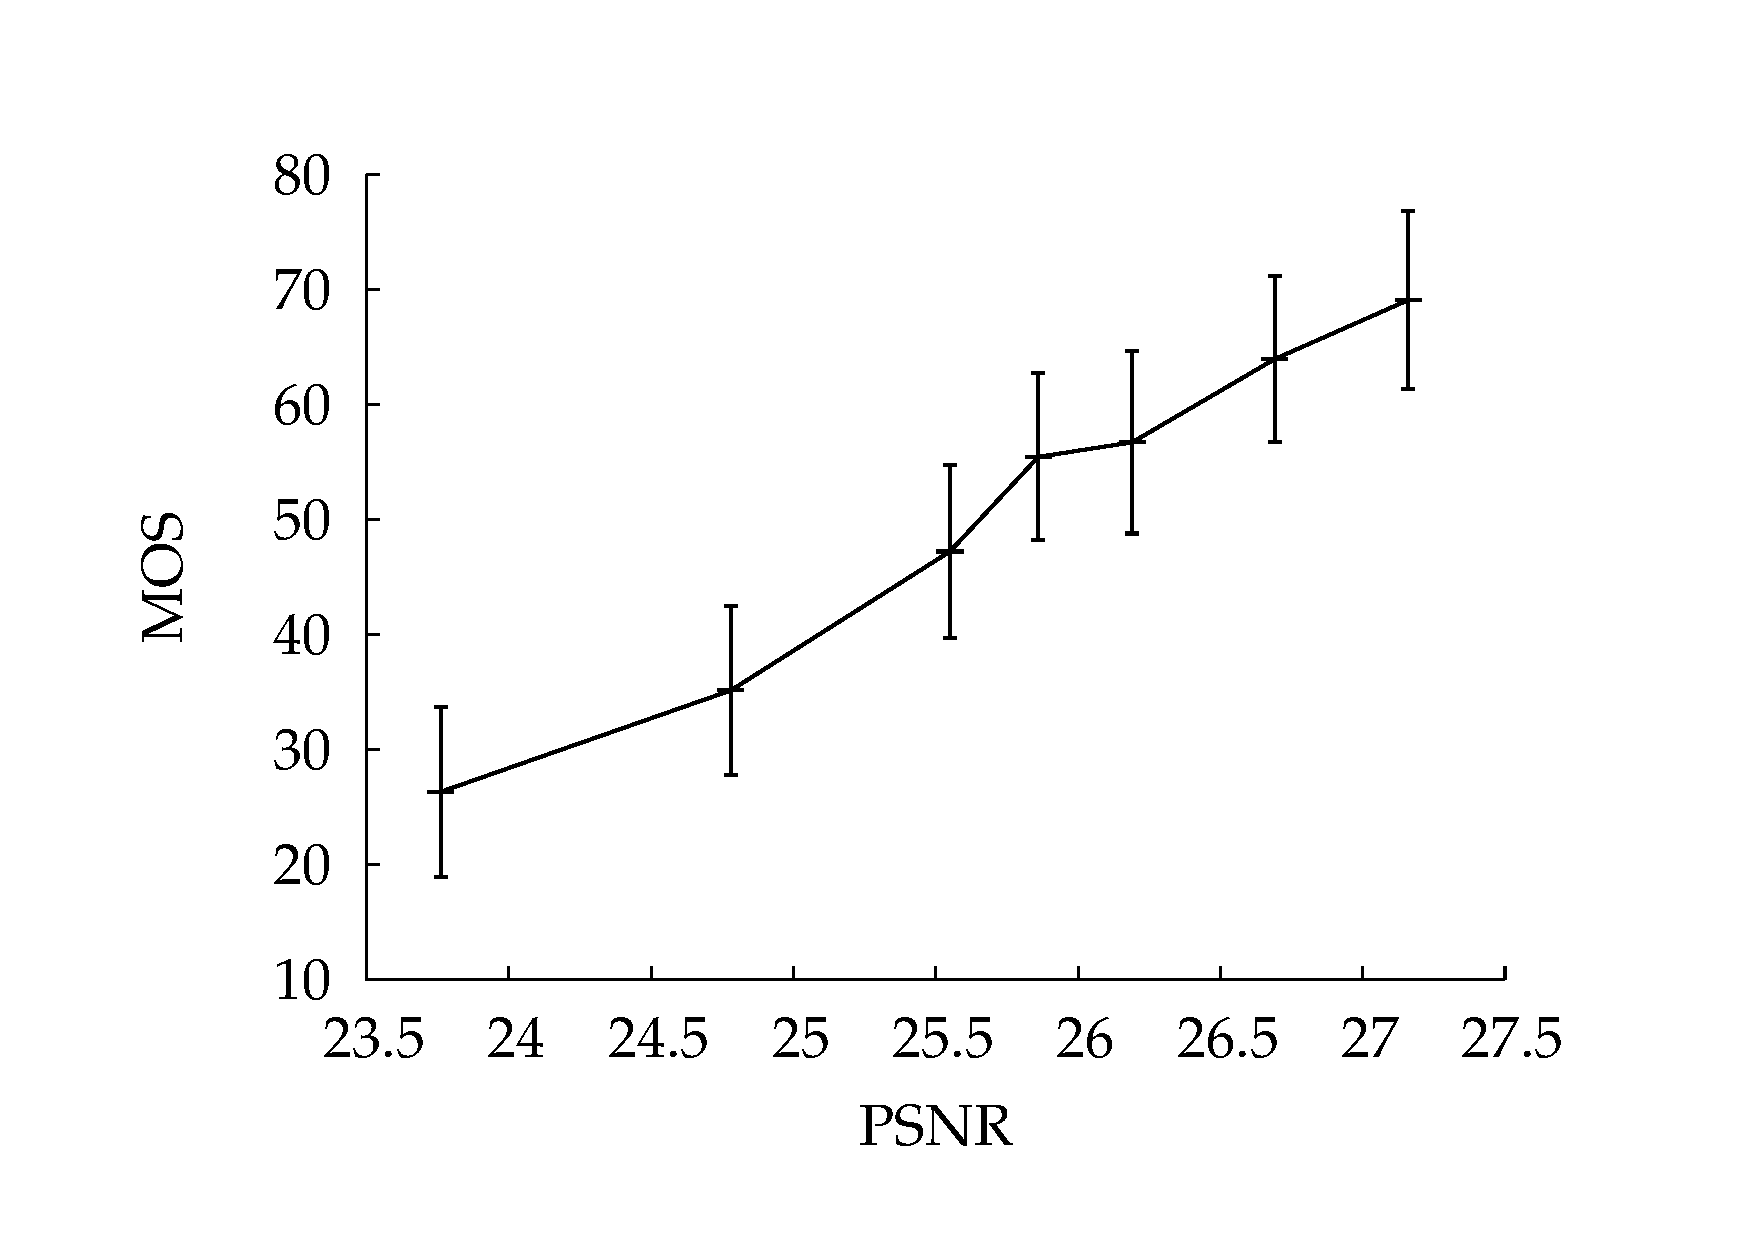
\includegraphics[width=0.48\linewidth, trim=80 25 110 82, page = 1]{plot/MOS-PSNR}}\hfill
	\subfloat[\label{fig:PSNR2} Séquence \emph{Duck Fly}.]{\includegraphics[width=0.48\linewidth, trim=80 25 110 82, page = 2]{plot/MOS-PSNR}}\\
	\subfloat[\label{fig:PSNR3} Séquence \emph{Voile}.]{\includegraphics[width=0.48\linewidth, trim=80 25 110 82, page = 3]{plot/MOS-PSNR}}\hfill
	\subfloat[\label{fig:PSNR123} Séquences \emph{Parkrun}, \emph{Duck Fly} et \emph{Voile}.]{\includegraphics[width=0.48\linewidth, trim=80 25 110 82, page = 4]{plot/MOS-PSNR}}\\
	\caption{MOS en fonction du PSNR (en dB) pour trois séquences différentes.}
\end{figure}

Cela étant, ces défauts ne sont pas systématiquement comblés par les autres critères de la littérature. En fait, peu s'avèrent réellement robustes dans toutes les situations. C'est pourquoi elles sont généralement spécialisées, comme peut l'être le PSNR, mais dans une moindre mesure.


\subsection{Application à un contexte limité}
L'exemple précédent délimite des conditions d'utilisation du PSNR. S'il est restreint à un contexte donné, il peut fournir une relation forte avec les MOS.  Rodrigues~\cite{rodrigues-pcs2007} l'utilise pour évaluer sa technique d'amélioration du codage MPEG-4 de l'erreur de prédiction du mouvement des images B. Il compare le PSNR moyen des images codées en mode B d'une séquence avec et sans l'usage de cette technique. Il effectue cette comparaison sur plusieurs contenus, mais il ne compare pas les PSNR d'un contenu à l'autre. De même, il calcule le PSNR sur les trois composantes couleurs pour mesurer le gain obtenu sur chacune d'elle, mais il ne compare pas les PSNR entre différentes composantes.

Les limites du PSNR sont, en l'occurence, bien prises en compte par Rodrigues. Son usage doit ainsi se limiter à des comparaisons où peu de conditions changent. Par exemple, le PSNR peut être utilisé pour mesurer le gain en débit obtenu par des algorithmes centrés sur une très petite partie d'un schéma de codage~\cite{merkle-eusipco2007}. À l'inverse, une régulation de débit basée sur le PSNR peut poser des problèmes, car aucun contrôle sur la qualité visuelle n'est alors effectué.


\subsection{Le PSNR amélioré}
Il existe quelques tentatives d'amélioration du PSNR, notamment le WSNR \emph{(Weighted signal to noise ratio)}~\cite{damera-ieee2000}. Cela consiste à appliquer une pondération du SNR par une CSF comme celle de Mannos et Sakrison~\cite{mannos-ieee1974}. Le calcul de l'erreur locale est ainsi plus pertinente, mais le problème du cumul n'est pas traité. Cette méthode permet de gagner en précision par rapport au SNR, mais sans atteindre les performances d'autres critères.

Oelbaum~\cite{oelbaum-pcs2007} propose une technique d'amélioration des critères de qualité en général et applicable entre autre au PSNR. Elle est basée sur l'observation que nous venons de faire : la corrélation entre les MOS et les notes objectives est forte dans le cas du codage à plusieurs débits d'un même contenu donné par un codeur donné. L'auteur exploite cette propriété pour réduire la différence entre la qualité prédite et la qualité subjective. La figure~\ref{fig:methodOelbaum} présente son modèle. La méthode nécessite la création de deux séquences additionnelles codées/décodées. La première doit être de haute qualité visuelle, entre 80 et 100 sur une échelle de 0 à 100. La seconde doit être de basse qualité, entre 0 et 20. Pour déterminer ces qualités, il faut donc effectuer des tests subjectifs. L'application de la méthode au PSNR est la suivante. Fixons les qualités subjectives des ancres de haute et basse qualité à 90 et 10 respectivement. Leurs PSNR sont $\mathit{PSNR}_h$ et $\mathit{PSNR}_b$ respectivement. Deux paramètres $\mathit{slope}$ et $\mathit{offset}$ sont calculés de la manière suivante :
\begin{equation}
\mathit{slope}=\frac{\mathit{PSNR}_h - \mathit{PSNR}_b}{90-10}\qquad \text{et}\qquad \mathit{offset} = \mathit{PSNR}_b - (10\times \mathit{slope}).
\end{equation}
%
Une fois ces paramètres connus, le PSNR amélioré d'une séquence dégradée, appelé PSNR$^+$, est calculé par :
\begin{equation}
\mathit{PSNR}^+ = \frac{\mathit{PSNR} - \mathit{offset}}{\mathit{slope}}
\end{equation}

\begin{figure}[htbp]
	\centering
	\begin{tikzpicture}[text centered, node distance = 3cm]% \begin{tikzpicture}[text centered, node distance = 3cm]
% Place nodes
	\node[text width=1.5cm] (ref) {séquence originale};
	\node[action, right of=ref, node distance = 2.2cm] (codage) {codage};
	\node[right of=codage, text width=2cm, node distance = 2.5cm] (deg) {séquence dégradée};
	\node[below of=deg, node distance = 2cm, text width=2cm, node distance = 2.5cm] (seqBas) {séquence de basse qualité};
	\node[below of=seqBas, node distance = 2cm, text width=2cm, node distance = 2.5cm] (seqHaut) {séquence de haute qualité};
	\node[action, right of=deg, text width=1.5cm] (critDeg) {critère de qualité};
	\node[action, right of=seqBas, text width=1.5cm] (critBas) {critère de qualité};
	\node[action, right of=seqHaut, text width=1.5cm] (critHaut) {critère de qualité};
	\node[below of=critBas, node distance = 1cm] (tmp) {};
	\node[action, right of=tmp, text width=3cm, rotate=90, node distance = 3.2cm] (regression) {régression};
	\node[action, right of=critDeg, node distance = 3.2cm] (correction) {correction};
	\node[right of=correction, node distance = 2cm] (psnr) {$\mathit{PSNR}^+$};

% Draw edges
	\path[fleche] (ref) -- (codage);
	\path[fleche] (codage) -- (deg);
	\path[fleche] (deg) -- (critDeg);
	\path[fleche] (codage) |- (seqBas);
	\path[fleche] (seqBas) -- (critBas);
	\path[fleche] (codage) |- (seqHaut);
	\path[fleche] (seqHaut) -- (critHaut);
	\path[fleche] (critBas) -- (regression) node[above=2pt,pos=0.5] {$\mathit{PSNR}_b$};
	\path[fleche] (critHaut) -- (regression) node[below=4pt,pos=0.5] {$\mathit{PSNR}_h$};
	\path[fleche] (critDeg) -- (correction) node[above,pos=0.5] {PSNR};
	\path[fleche] (regression) -- (correction) node[right,pos=0.5] {$\mathit{slope, offset}$};
	\path[fleche] (correction) -- (psnr);
% \end{tikzpicture}
\end{tikzpicture}
	\caption{Schéma de la technique d'amélioration des critères de qualité d'Oelbaum~\cite{oelbaum-pcs2007}.}
	\label{fig:methodOelbaum}
\end{figure}

L'auteur évalue les performances de sa méthode sur un ensemble de 54 séquences CIF dégradées par un codage H.264 et évaluées par 20 observateurs. Il ne précise pas les paramètres de codage de ces séquences. Les ancres basse et haute sont codées par le codeur de référence H.264~\cite{h264-jm} en fixant les pas de quantification pour chacune. L'auteur ne précise pas non plus si les performances qu'il fournit sont calculées après l'application d'une fonction d'ajustement. Une telle fonction permet de transformer les PSNR$^+$ en une prédiction du MOS, appelé MOSp. Le coefficient de corrélation entre les MOS et les PSNR$^+$ est de 0,831 alors qu'il est de 0,665 avec un simple PSNR. L'\emph{outlier ratio} des PSNR$^+$ est de 0,722, alors qu'il est de 0,907 pour les PSNR. Cet indicateur calcule le rapport $\frac{N_{e}}{N_n}$ entre le nombre de configurations mal évaluées $N_e$ et le nombre total de notes objectives $N_n$. Une configuration est considérée comme mal évaluée si $|\MOS - \MOSp| > 2\times\IC$ avec $\IC$ l'intervalle de confiance à 95\% du MOS. Le gain est significatif, sans pour autant suffire à rendre le PSNR très robuste.

Outre ce gain en performance insuffisant dans le cas du PSNR, cette approche originale a d'autres désavantages. Le premier est qu'elle nécessite la création de nouvelles séquences, dont il faut évaluer la qualité de manière subjective pour que la régression linéaire soit efficace. Cela peut être fait par des experts sans mettre en place un ensemble de tests psychophysiques mais nécessite tout de même une intervention, ce qui réduit l'automatisation de la méthode. De plus, pour créer ces ancres basse et haute, l'auteur conseille d'utiliser un codeur proche, en termes de technologie, de celui utilisé pour coder les séquences évaluées. Enfin, dans le cas plus général de l'utilisation de cette méthode avec des critères de qualité vidéo sans référence, elle nécessite tout de même les paramètres $\mathit{slope}$ et $\mathit{offset}$. En conséquence, un critère sans référence devient avec référence réduite, celle-ci étant constituée de ces deux paramètres.


\section{Approches basées sur la modélisation fine de la vision humaine bas niveau}
Ce type d'approche cherche à modéliser plus ou moins finement les phénomènes bas niveau de la vision. Les connaissances nécessaires à cette modélisation sont le plus souvent issus d'expérimentations psychovisuelles. La complexité du système de vision humaine fait que ces travaux durent depuis de nombreuses années. Les premiers résultats portaient sur l'image fixe, avant de s'intéresser plus récemment à la vidéo.


\subsection{Métriques de qualité en images fixes}
Le schéma classique de la version la plus évoluée d'une telle métrique est donné sur la figure~\ref{fig:ApprocheSVH}. Historiquement, les différents éléments qui le constitue sont apparus progressivement.

\begin{figure}[htbp]
	\centering
	\begin{tikzpicture}[text centered, node distance = 3cm]% \begin{tikzpicture}[text centered]
% Place nodes
	\node[text width=2cm] (ref) {séquence originale};
	\node[action, below of=ref, text width=2.5cm, node distance = 2.4cm] (couleur) {décomposition dans un espace de couleurs antagonistes};
	\node[below of=couleur, text width=2cm, node distance = 2.4cm] (deg) {séquence dégradée};
	\node[action, right of=couleur, text width=2cm] (csf) {fonction de sensibilité aux contrastes};
	\node[action, right of=csf, text width=2.5cm] (canaux) {décomposition en canaux perceptuels};
	\node[action, right of=canaux, text width=2cm] (masq) {fonction de masquage};
	\node[action, right of=masq, node distance = 2cm] (cumul) {cumul};
	\node[right of=cumul, node distance = 1.5cm] (note) {note};

% Draw edges
	\path[fleche] (ref) -- (couleur);
	\path[fleche] (deg) -- (couleur);
	\path[fleche] (couleur) -- (csf);
	\path[fleche] (csf) -- (canaux);
	\path[fleche] (canaux) -- (masq);
	\path[fleche] (masq) -- (cumul);
	\path[fleche] (cumul) -- (note);
% \end{tikzpicture}\end{tikzpicture}
	\caption{Schéma générique d'une métrique de qualité basée sur la modélisation fine de la vision humaine bas niveau.}
	\label{fig:ApprocheSVH}
\end{figure}

Les premières modélisations du système visuel humain reposent sur une approche à un seul canal perceptuel. Dans les travaux de Mannos, seule une fonction de sensibilité aux contrastes (CSF) permet de définir le système~\cite{mannos-ieee1974}. Une CSF décrit l'évolution de la sensibilité visuelle en fonction des fréquences spatiales et de l'orientation du signal à détecter. La sensibilité visuelle est définie comme l'inverse du contraste d'un signal à son seuil différentiel de visibilité.

Un élément important de la perception est l'effet de masquage. Celui-ci se caractérise par la modification de la perception d'un signal par la présence d'un autre signal. En pratique, cela consiste à prendre en considération le contexte spatial et temporel dans le calcul d'une mesure locale comme un contraste. L'inclusion de ces effets de masquage dans les métriques de qualité mono-canal a permis de sensiblement les améliorer~\cite{kusayama-pcs2001}.

Les effets de masquage sont mieux caractériser par les modélisations multi-canaux que par les modélisations mono-canal car ils permettent d’intégrer certaines spécificités des champs récepteurs du système visuel. Zetzsche~\cite{zetzsche-vcip1989} propose le premier modèle utilisant une décomposition en canaux perceptuels. Celle-ci utilise une pyramide ROG \emph{(ratio of gaussian)} à cinq niveaux de résolution et un ensemble de filtres gaboriens ayant une sélectivité angulaire de 30 degrés. Plusieurs types de décomposition ont été proposés. Par exemple, le VDP de Daly~\cite{daly-vdp} utilise une version adaptée de la transformée Cortex de Watson~\cite{watson-cortex}. Celle-ci se caractérise par des filtres à sélectivité radiale dyadique et à sélectivité angulaire de 30 degrés. Lubin~\cite{lubin-jnd} décompose les images originales et dégradées en sous-bandes à l'aide de sept filtres passe-bandes de fréquences centrales allant de 32 à 0,5 cycle par degré. Une décomposition pyramidale à cinq niveaux permet ensuite de créer un ensemble d'images de plusieurs résolutions.

Le premier critère de qualité d'images en couleur a été proposé par Faugeras~\cite{faugeras-ieee1979}. À partir de la réponse des cônes de la rétine, il effectue une décomposition dans un espace couleur perceptuel. Il obtient ainsi une composante achromatique et deux composantes chromatiques. Ce calcul repose sur la théorie classique des signaux antagonistes, largement utilisé~\cite{lambrecht-cmpqm,lai-perceptual,krauskopf-vr1982}. L'\oe il humain étant plus sensible à la luminance qu'à la chrominance, il est courant de donner moins d'importance ou de précision à cette dernière. C'est par exemple le cas de la décomposition en canaux de Le Callet~\cite{lecallet-phd} qui limite le plan fréquentiel des composantes chromatiques aux deux premières bandes de fréquences spatiales, alors que celui de la composante achromatique en compte quatre. De même, le cumul inter-composante exploite cette propriété en privilégiant la luminance.

La dernière étape de cumul est très importante dans la mesure où elle permet d'obtenir la note de qualité finale à partir des contributions locales. Cependant, ce cumul est souvent simplifié car la manière dont il est opéré par le système visuel humain n'est toujours pas bien connue~\cite{wang-ovqa}. Peu d'originalité en découle, les auteurs préférant privilégier les étages précédents. La sommation de Minkowski est alors souvent utilisée pour intégrer les mesures locales. Cette sommation est de la forme :
\begin{equation}
S_M = \left( \frac{1}{N_v} \sum\limits_{i=1}^{N_v} v_i^\beta \right)^{\frac{1}{\beta}}
\end{equation}
%
avec $\beta$ l'exposant de la sommation et $v$ le vecteur de $N_v$ éléments. Cependant, cette somme ne permet de pondérer les données qu’en fonction de leur amplitude et non en fonction de leur répartition spatiale ou temporelle~\cite{wang-icassp2002}. La complexité des phénomènes haut niveau mis en jeu lors de la construction finale de la note subjective de qualité n'est donc pas entièrement considérée.


\subsection{Passage à la vidéo}
La conception de critères objectifs de qualité adaptés à la vidéo pose l'épineux problème de la dimension temporelle. Celle-ci implique des modifications à la fois au niveau du calcul des erreurs locales et de leur cumul en une note de qualité. Ce type de métrique de qualité vidéo peut ainsi se décomposer en deux étages principaux comme le montre la figure~\ref{fig:ApprocheSVHVideo}.

\begin{figure}[htbp]
	\centering
	\begin{tikzpicture}[text centered, node distance = 3cm]% \begin{tikzpicture}[text centered]
% Place nodes
	\node[text width=2cm] (ref) {séquence originale};
	\node[action, right of=ref, text width=3cm, node distance = 3.5cm] (mesure) {mesure des erreurs locales};
	\node[action, right of=mesure] (cumul) {cumul};
	\node[right of=cumul, node distance = 2cm] (note) {note};

% Draw edges
	\path[fleche] (ref) -- (mesure);
	\path[fleche] (mesure) -- (cumul);
	\path[fleche] (cumul) -- (note);
% \end{tikzpicture}\end{tikzpicture}
	\caption{Les deux étages principaux d'un critère de qualité vidéo.}
	\label{fig:ApprocheSVHVideo}
\end{figure}

Il est courant que les critères d'évaluation de la qualité vidéo soient adaptés de critères pour images fixes. Ainsi, Watson adapte sa DCTune~\cite{watson-dctune} pour proposer la DVQ~\cite{watson-dvq}. Les éléments de vision qu'il intègre sont assez nombreux : adaptation en luminance, décomposition en composantes couleur, décomposition spatio-fréquentielle, filtrage spatial et temporel et masquage de contraste. Le point intéressant est le passage de la notion de visibilité de bruit DCT de l'image à la vidéo. L'auteur intègre pour cela un modèle mathématique qui s'adapte aux seuils de visibilité pour rendre compte du mouvement. Ce modèle établit un seuil pour chaque fonction DCT de base 8\texttimes8. Les paramètres mathématiques ont été déterminés par des simulations de stimuli de bruit DCT dynamique. À partir d'expériences psychophysiques, Watson propose un modèle tridimensionnel séparable, produit d'une fonction temporelle, d'une fonction spatiale et d'une fonction d'orientation. Le cumul final est effectué par une sommation de Minkowski.

Le premier modèle de vision connu est celui de Lukas et Budrikis~\cite{lukas-PQMonVM}, adaptée à la télévision noir et blanc. Il incorpore deux éléments principaux. Le premier est un modèle spatio-temporel non linéaire permettant de filtrer les erreurs de la séquence dégradée. La non linéarité agit comme un contrôle du gain, permettant au modèle de s'adapter aux changements de niveau de luminance de fond. Le second élément est une fonction de masquage. Le stimulus d'entrée est pondéré suivant la quantité d'activité spatio-temporelle locale. Enfin, la mesure de distorsion est calculée par la norme $L_p$ de l'image des erreurs masquées. Les auteurs montrent que les observateurs basent leur jugement sur l'évaluation de zones critiques plutôt que sur l'ensemble de la séquence. Ils justifient ainsi la pertinence de la mesure d'erreurs locales. Cependant, le cumul appliqué à ces erreurs est une simple moyenne, ce qui ne rend le résultat final beaucoup moins pertinent.

Plus récemment, Winkler a proposé la PDM \emph{(Perceptual distortion metric)}~\cite{winkler-hvei1999} pour l’évaluation de qualité de séquences d’images couleur. Il s'agit d'une amélioration de la NVFM \emph{(Normalized video fidelity metric)} de Lambrecht~\cite{lindh-icip1996}. Après la décomposition des composantes couleur, la décomposition perceptuelle est effectuée dans le temps, puis dans l'espace. L'aspect temporel est considéré comme décomposable par un filtre passe-bas, fournissant le canal \emph{sustained} et un filtre passe-bande, produisant le canal \emph{transient}. Les filtres utilisés sont modélisés par deux filtres à réponse impulsionnelle infinie, plus adaptés que des filtres à réponse finie en termes de temps de réponse et de précision. Le filtre passe-bas est appliqué aux trois composantes couleur, alors que le filtre passe-bande n'est appliqué qu'à la composante achromatique. L'auteur justifie cette pratique par le fait que la sélectivité au contraste chromatique est faible dans les hautes fréquences temporelles. Cela permet également de réduire la complexité du traitement. Après les décompositions spatiale et temporelle, le signal en sortie chaque canal est pondéré afin que l’ensemble des filtres approxime la courbe de sensibilité spatio-temporelle du système visuel. L'auteur reconnait que la séparabilité des domaines spatial et temporel est problématique. Il traite cette question en ajustant ses filtres de façon à ce que la prédiction obtenue par le modèle corresponde aux résultats d'expériences de sensibilité au contraste spatio-temporel. À nouveau, le cumul final est effectué par des sommations de Minkowski, en séparant les cumuls fréquentiel et spatial. Les exposants sont 2 pour le cumul spatial et 4 pour le cumul temporel, donnant ainsi plus d'importance aux images temporelles plus dégradées.

En fait, nous constatons que les critères de qualité vidéo privilégient grandement le calcul des mesures locales par rapport à leur cumul qui reste très simple, voire simpliste. La sommation de Minkowski est utilisée par de nombreux autres modèles~\cite{deridder-spie1992,lindh-icip1996,lubin-jnd,masry-spic2004}, autant pour l'intégration temporelle que des mesures locales. Cependant, elle ne permet de pondérer les données qu’en fonction de leur amplitude et non en fonction de leur répartition spatiale ou temporelle~\cite{wang-icassp2002}. La complexité des phénomènes haut niveau mis à contribution lors de la construction de la mesure subjective n'est donc pas pleinement considérée. Comme exemple de méthode de cumul plus élaboré, citons des travaux précédents~\cite{lecallet-ieee2006}. Nous nous sommes intéressés particulièrement au cumul temporel, utilisant des caractéristiques de qualité de la littérature. Pour cela, nous avons utilisé un réseau de neurones à convolution qui intègre les caractéristiques par tranches temporelles avant de les intégrer temporellement. Le réseau est ainsi bien adapté à l'évaluation continue de la qualité. Dans cette étude, nous disposions de l'évaluation continue de quatre séquences de trois minutes. Cette méthode s'est montrée efficace et est utilisable avec référence réduite à partir des caractéristiques extraites des séquences de référence et dégradée, mais aussi sans référence en utilisant celles de la séquence dégradée. L'usage de l'évaluation continue de la qualité permet d'obtenir suffisamment de données pour rendre pertinente l'utilisation du réseau. Cela n'est pas contre pas possible avec d'autres méthodologies.

Au final, la problématique du cumul reste peu prise en compte dans les critères de qualité vidéo car elle est encore mal comprise. Malheureusement, cela ne permet pas de tirer tout le bénéfice des élaborations des étages précédents, aussi raffinés soient-ils. En fait, il est illusoire de privilégier un seul des éléments de la figure~\ref{fig:ApprocheSVHVideo}. Chacun doit être caractérisé en détail car c'est le moins performant qui limitera les performances de l'ensemble.


\subsection{Performances et limites}
\subsubsection{VQEG Phase 1 : comparaison de critères}
Comparer des métriques de qualité nécessite d'importantes ressources. Le rassemblement de matériel et de contenu, la génération et l'évaluation subjective des séquences, et enfin la production de notes objectives de qualité à partir des modèles est une tâche extrêmement complexe. Le groupe de normalisation VQEG s'est chargé d'évaluer une dizaine de critères de qualité avec référence complète pour la télévision~\cite{vqeg-frtv1}. Il s'agissait de la première expérience menée par le groupe d'experts, c'est pourquoi elle est nommée Phase 1. Cette évaluation a permis des avancées significatives dans le domaine de l'évaluation de la qualité vidéo. La mise à disposition des notes subjectives et des séquences est d'un grand intérêt scientifique pour la communauté de la qualité vidéo.

Parmi les critères évalués où figure également le PSNR, six reposent sur une modélisation plus ou moins poussée de la vision humaine bas niveau :
\begin{itemize}
\item le modèle de Sarnoff est la suite des travaux de Lubin. Il est basé sur un modèle de discrimination visuelle qui simule la réponse à un signal vidéo des mécanismes spatio-temporels du système visuel humain. La mesure de qualité est calculée à partir des différences perceptuelles entre les réponses de la séquence d'origine et de la séquence dégradée.
\item le modèle du NHK utilise des filtres spatio-temporels pour émuler les caractéristiques de la vision humaine. Ils sont appliqués sur les différences entre la séquence originale et la séquence dégradée. La mesure finale est une pondération des mesures issues des filtres.
\item le modèle de l'ÉPFL est le PDM de Winkler~\cite{winkler-hvei1999}.
\item le modèle de Tapestries consiste en deux parties : un modèle perceptuel et une extraction de caractéristiques. Le modèle perceptuel simule le système visuel humain et pondère les dégradations suivant leur visibilité. Il inclut une mesure de contraste, un filtrage spatial et une pondération tenant compte de l'orientation. L'extraction de caractéristiques mesure uniquement l'effet de bloc. Les deux parties fournissent une mesure de qualité. L'une ou l'autre des mesures est retenue comme mesure finale de la qualité, suivant le résultat de l'extraction.
\item le modèle de la NASA est la DVQ de Watson~\cite{watson-dvq}.
\item le modèle de KPN comporte trois étapes. La première est une CSF appliquée sur les composantes de luminance et de chrominance. La seconde extrait les contours de luminance à l'aide d'un filtre de Sobel. Une mesure globale des contours est obtenue en moyennant les mesures sur l'espace et le temps. La troisième étape est un calcul d'erreur de chrominance à partir des composantes Cr et Cb. Enfin, les indicateurs obtenus sont cumulés en une note de qualité.
\end{itemize}

L'ensemble de séquences utilisé est constitué de 24 contenus différents. Chacun est dégradé par 16 traitement différents. Afin de comparer les performances des critères de qualité, des indicateurs sont utilisés. Le tableau~\ref{tab:resultatsVQEGPhase1} présente les résultats de deux de ces indicateurs, obtenus sur l'ensemble des séquences. L'indicateur 1 est le coefficient de corrélation de rang calculé entre les MOS et les notes objectives issues des modèles, notées MOSp. Tapestries explique la très faible valeur qu'il obtient par des problèmes techniques. L'indicateur 2 est l'\emph{outlier ratio}. Pour chaque indicateur, des tests statistiques permettent de déterminer si la différence entre deux critères est significative.

\begin{table}[htbp]
\centering
\begin{tabular}[c]{cccccccc}\toprule
\strong{critère} & \strong{PSNR} & \strong{Sarnoff} & \strong{NHK} & \strong{ÉPFL} & \strong{Tapestries} & \strong{NASA} & \strong{KPN} \\ \toprule
indicateur 1 & 0,786 & 0,792 & 0,718 & 0,784 & 0,248 & 0,786 & 0,803 \\ \midrule
indicateur 2 & 0,678 & 0,656 & 0,725 & 0,611 & 0,844 & 0,636 & 0,578\\ \bottomrule
\end{tabular}
\caption{Performances des critères basés sur la modélisation de la vision humaine dans la première campagne d'évaluation de critères de qualité pour la télévision de VQEG~\cite{vqeg-frtv1}.}
\label{tab:resultatsVQEGPhase1}
\end{table}

La première surprise est que le PSNR obtient des performances statistiquement équivalentes aux autres. Les experts de VQEG Phase 1 expliquent cela par le fait que les conditions testées sont très nombreuses. Ainsi, chaque critère se retrouve défavorisée dans une ou plusieurs conditions, ce qui tend à faire chuter ses performances. Au contraire, le PSNR reste globalement moyen. L'autre explication avancée est que les séquences ont été réalignées et normalisées avant le calcul du PSNR. Or le désalignement est un phénomène très mal prédit par le PSNR. Pourtant, toutes les métriques ont bénéficié de ce traitement. Enfin, les tests subjectifs ont tous été réalisés dans les mêmes conditions, avec le même type d'écran et la même procédure. Alors que le PSNR serait incapable de s'adapter à des changements de ces conditions, VQEG Phase 1 considère que les autres modèles pourraient y gagner en performances face au PSNR.

La seconde surprise est qu'en fait, tous les critères se sont avérés statistiquement équivalents. En conséquence, VQEG Phase 1 fut dans l'incapacité d'en proposer un en vue de sa normalisation, même en restreignant les critères à un sous-ensemble de conditions. La conclusion finale de cette campagne est qu'aucun des critères proposés ne fut capable de remplacer l'évaluation subjective de la qualité.


\subsubsection{Des modèles limités}
L'utilisation seule de ces modèles bas niveau, aussi sophistiqué soient-ils, ne suffit donc pas à refléter la perception de la qualité par le système visuel humain. La raison principale est l'absence de considérations de haut niveau. Nous savons par exemple que la tâche influe sur l'évaluation de la qualité de l'observateur moyen~\cite{fuhrmann-jei1995}. Les aspects comme l'attention, l'intérêt ou la construction du jugement affectent également l'évaluation de qualité. Frater~\cite{frater-ieee2001} a étudié la différence entre la sensibilité aux dégradations présentes à l'arrière-plan et celles au premier plan dans un environnement de vidéoconférence. Il montre que cette différence augmente quand le discours de la personne au premier plan est diffusé. Enfin, alors que la modélisation des mécanismes bas niveau est bien maitrisée au niveau local, leur combinaison en une note de qualité globale n'est pas encore très bien connue. En pratique, elle se réduit la plupart du temps à une sommation de Minkowski qui permet de pondérer les données en fonction de leur amplitude. Cette méconnaissance est particulièrement problématique et ruine en grande partie les efforts apportés aux autres éléments de l'approche.

Tektronix~\cite{ferguson-vpqm2007} est la dernière société à continuer dans cette voie, avec un modèle très poussé. Il ne considère cependant pas ces aspects haut niveau. Leur impact sur la qualité perçue, leur importance par rapport aux éléments actuellement considérés et la manière de les intégrer dans un modèle d'évaluation de la qualité sont autant de question qui restent en suspens.


\section{Approches basées sur la fidélité structurelle}
Les critères adoptant cette approche sont plus récents. Ils se basent non pas sur des propriétés bas niveau de la vision, mais sur des propriétés supposées haut niveau portant sur la réaction du système visuel humain à une image dégradée. La principale hypothèse est que notre perception est particulièrement adaptée à l'extraction de l'information structurelle d'une image. L'idée est donc de mesurer les dégradations de cette information structurelle.

La première mesure ayant utilisé ce concept est la SSIM \emph{(Structural similarity)} de Wang et Bovik~\cite{wang-ssim}, adaptée à l'évaluation de qualité des images fixes. Quelques contributions ont par la suite apporté des améliorations à la version originale, et notamment son adaptation à la vidéo. En quelques années, SSIM est devenue assez utilisée, surtout par la communauté universitaire américaine, car elle allie une simplicité de mise en \oe uvre et des performances supérieures au PSNR. D'autres métriques utilisent des principes similaires que nous allons maintenant détailler.


\subsection{SSIM : index de similarité structurelle} \label{ssec:ssim}
L'index de similarité SSIM utilise l'index de qualité d'image UQI \emph{(Universal image quality index)} des mêmes auteurs~\cite{wang-uiqi}. Cet index UIQI définit des mesures de comparaison de luminance $l(x,y)$, de contraste $c(x,y)$ et de structure $s(x,y)$ entre deux signaux $x$ et $y$ de luminance :
\begin{equation}
l(x,y) = \dfrac{2\mu_x \mu_y}{\mu_x^2 + \mu_y^2} , \qquad c(x,y) = \dfrac{2\sigma_x \sigma_y}{\sigma_x^2 + \sigma_y^2}, \qquad s(x,y) = \dfrac{\mathit{cov}_{xy}}{\sigma_x \sigma_y}
\end{equation}
%
avec $\mu_x$ la moyenne de $x$, $\mu_y$ la moyenne de $y$, $\sigma_x^2$ la variance de $x$, $\sigma_y^2$ la variance de $y$ et $\mathit{cov}_{xy}$ la covariance entre $x$ et $y$. L'index de similarité UQI entre $x$ et $y$ correspond alors à :
\begin{equation}
\text{UQI}(x,y) = l(x,y) \times c(x,y) \times s(x,y) = \dfrac{4\mu_x\mu_y\mathit{cov}_{xy}}{(\mu_x^2+\mu_y^2)(\sigma_x^2 + \sigma_y^2)}
\end{equation}

Le passage à SSIM~\cite{wang-ssim} résulte de la prise en compte des cas où $\mu_x^2+\mu_y^2$ ou $\sigma_x^2 + \sigma_y^2$ peuvent être proches de zéro. La formule est alors transformée de la manière suivante :
\begin{equation}
\text{SSIM}(x,y) = \dfrac{(2\mu_x\mu_y+c_1)(2\mathit{cov}_{xy}+c_2)}{(\mu_x^2+\mu_y^2 + c_1)(\sigma_x^2 + \sigma_y^2 + c_2)}
\end{equation}
%
avec $c_1 = (k_1L)^2$, $c_2 = (k_2L)^2$, $L$ la dynamique des valeurs des pixels, soit 255 pour des images codées sur 8 bits, $k_1$ = 0,01 et $k_2$ = 0,03 par défaut.

Pour l'évaluation de qualité d'une image, la formule précédente est appliquée sur la luminance uniquement. Typiquement, les grandeurs sont calculées sur des fenêtres de taille 8\texttimes8. La fenêtre courante peut se déplacer pixel par pixel sur l'ensemble de l'image. Cependant, les auteurs proposent de ne considérer qu'un sous-ensemble de ces fenêtres, par exemple en réduisant leur nombre d'un facteur deux dans les deux dimensions. Ceci permet de diminuer la complexité du calcul. La carte de mesures SSIM obtenue peut laisser apparaitre des effets de bloc indésirables. Pour limiter cet effet, les auteurs utilisent une fonction de pondération $w = \{w_i|i=1,2,\dots,N_w\}$ gaussienne, circulaire, symétrique, de taille 11\texttimes11, d'écart-type 1,5 et de somme $\sum_{i=1}^{N_w}w_i=1$. Les grandeurs précédentes sont alors :
\begin{equation}
\mu_x = \sum\limits_{i=1}^{N_w} w_i x_i , \quad \mu_y = \sum\limits_{i=1}^{N_w} w_i y_i, \quad \sigma_{xy} = \sum\limits_{i=1}^{N_w} w_i(x_i-\mu_x)(y_i-\mu_y),
\end{equation}
\begin{equation}
\mu_x = \sum\limits_{i=1}^{N_w} w_i x_i , \quad \mu_y = \sum\limits_{i=1}^{N_w} w_i y_i, \quad \sigma_{xy} = \sum\limits_{i=1}^{N_w} w_i(x_i-\mu_x)(y_i-\mu_y),
\end{equation}
\begin{equation}
\sigma_x = \left(\sum\limits_{i=1}^{N_w} w_i(x_i-\mu_x)^2\right)^{\frac{1}{2}}, \quad \sigma_x = \left(\sum\limits_{i=1}^{N_w} w_i(y_i-\mu_y)^2\right)^{\frac{1}{2}}.
\end{equation}
%
Enfin, la métrique de qualité MSSIM entre les images $X$ et $Y$ est la moyenne des mesures SSIM sur les $N_f$ fenêtres de la luminance de l'image :
\begin{equation}
\text{MSSIM}(X,Y) = \frac{1}{N_f} \sum\limits_{i=1}^{N_f} \text{SSIM}(x_i,j_i).
\end{equation}

Les auteurs évaluent les performances de leur métrique sur une base de 29 images originales. Les images dégradées sont obtenues par codage/décodage JPEG ou JPEG2000. Un total de 175 images JPEG et 169 images JPEG2000 sont évaluées par un panel de 13 à 25 observateurs suivant les sessions. Ces images forment la première version de la base LIVE~\cite{sheikh-live}, connue pour être la première base d'images fixes mise à disposition de la communauté avec les MOS de chaque image. Celles-ci sont en couleur, mais seule la luminance est utilisée pour la construction de la métrique. En effet, les auteurs ne remarquent pas d'améliorations sensibles en utilisant les composantes de chrominance. Le coefficient de corrélation entre les MOS et les notes objectives issues du modèle est de 0,967. En comparaison, le coefficient de corrélation avec le PSNR est de 0,905 et de 0,956 avec le modèle de Sarnoff.

Il est étonnant de constater que le PSNR soit aussi fortement corrélé avec les évaluations subjectives sur une base de 344 images. La seconde version de la base~\cite{sheikh-ip2006} comporte 779 images. Sur ce nouvel ensemble, le coefficient de corrélation du PSNR avec le MOS est de 0,8709. Ces valeurs sont très supérieures à celles couramment constatées~\cite{oelbaum-pcs2007} sur une telle quantité d'image. Les très bons résultats du PSNR peuvent laisser penser que les images utilisées ne sont pas suffisamment représentatives pour évaluer correctement le PSNR.

Signalons également que la relation entre les mesures de similarité globale et les MOS est non linéaire. La fonction MOS $= f(\text{SSIM})$ est de type exponentielle. %Ainsi, le coefficient de corrélation fournit par les auteurs est non linéaire.
La conséquence est qu'une faible variation de la mesure de similarité peut entrainer une importante erreur de prédiction du MOS. Or, de nombreux facteurs interviennent dans le calcul de la mesure et sont donc susceptibles de provoquer de telles variations.


\subsection{Améliorations et adaptation à la vidéo de SSIM}
Plusieurs critères de qualité ont été créés à partir de SSIM. Chen en propose deux très proches. Le premier est le ESSIM \emph{(Edge-based SSIM)}~\cite{chen-icassp2006}. L'unique changement porte sur la grandeur de structure $s$. Elle est remplacée par une mesure de comparaison des contours $e$. La première étape de l'algorithme est de calculer les cartes de gradient des images originale et dégradée à l'aide de deux filtres de Sobel. À partir de ces cartes, la direction et l'amplitude du gradient de chaque pixel de l'image sont calculés. Pour chaque fenêtre de calcul de l'index, les directions des pixels sont quantifiées selon huit directions discrètes, également réparties entre 0 et 180 degrés. Les vecteurs $\Upsilon_x$ et $\Upsilon_y$ sont les histogrammes de ces directions pour les images original et dégradée respectivement. La mesure de comparaison des contours est alors :
\begin{equation}
e(x,y) = \frac{\mathit{cov}(\Upsilon_x,\Upsilon_y) + c_3}{\sigma(\Upsilon_x)\cdot\sigma(\Upsilon_y) + c_3}
\end{equation}
%
avec $c_3$ une constante pour les cas où $\sigma(\Upsilon_x)\cdot\sigma(\Upsilon_y)$ est proche de zéro, $\sigma^2(\Upsilon_x)$ et $\sigma^2(\Upsilon_y)$ les variances des vecteurs $\Upsilon_x$ et $\Upsilon_y$ respectivement et $\mathit{cov}(\Upsilon_x, \Upsilon_y)$ la covariance entre les vecteurs $\Upsilon_x$ et $\Upsilon_y$.

Le second critère de Chen~\cite{chen-icip2006} est le GSSIM \emph{(Gradient-based SSIM)}. Il utilise le même principe mais modifie également la grandeur de contraste $c$. Celle-ci est calculée avec les écart-types des vecteurs $\Upsilon_x$ et $\Upsilon_y$. L'auteur compare ses métriques avec l'originale et le PSNR sur des sous-parties de la base LIVE. ESSIM est évaluée sur 489 images et GSSIM sur 779. Dans les deux cas, les performances des métriques proposées sont supérieures à celles de SSIM. Cela montre que prendre en compte l'activité du voisinage de calcul permet de mieux caractériser la structure de l'image.

L'extension de SSIM à la vidéo~\cite{wang-vqasdm} est proposée par les auteurs de SSIM eux-mêmes. La figure~\ref{fig:VSSIM} en présente la structure.

\begin{figure}[htbp]
	\centering
	\begin{tikzpicture}[text centered, text width=2cm,node distance=3cm]% \begin{tikzpicture}
\node (ref) {vidéo de référence};
\node[below of=ref,node distance=1.5cm] (tmp) {};
\node[below of=tmp,node distance=2cm] (deg) {vidéo dégradée};
\node[action, right of=deg,text width=1.5cm] (ssim) {calcul SSIM};
\node[action, right of=ssim,node distance=3.5cm] (cumulImage) {cumul sur l'image $i$};
\node[action, right of=cumulImage] (cumulSeq) {cumul sur la séquence};
\node[right of =cumulSeq,text width=1.2cm,node distance=2.5cm] (vssim) {VSSIM};
\node[action, above of=cumulImage,node distance=2cm] (calculw) {calcul de $w_{\mathit{ij}}$};
\node[action, right of=calculw] (calculW) {calcul de $W_i$};

\path[fleche] (ref) -| (calculw) node[right=-0.2cm, pos=0.7] {luminance};
\path[fleche] (calculw) -- (cumulImage) node[right=-0.8cm,pos=0.5] {$w_{\mathit{ij}}$};
\path[fleche] (calculW) -- (cumulSeq) node[right=-0.8cm,pos=0.5] {$W_i$};
\path[fleche] (deg) -- (ssim);
\path[fleche] (ssim) -- (cumulImage) node[below,pos=0.5] {$\text{SSIM}_{\mathit{ij}}$};
\path[fleche] (cumulImage) -- (cumulSeq) node[below,pos=0.5] {$Q_i$};
\path[fleche] (cumulSeq) -- (vssim);
\path[fleche] (ref) -| (ssim);
\path[fleche] (ref) -| (calculW) node[right,pos=0.7] {vecteurs de mouvement};

% \end{tikzpicture}
\end{tikzpicture}
	\caption{Structure du critère de qualité vidéo VSSIM.}
	\label{fig:VSSIM}
\end{figure}

Plusieurs adaptations sont à appliquer avant d'obtenir la métrique que nous nommerons VSSIM. Tout d'abord, Wang utilise ici les trois composantes couleurs. L'index SSIM est donc calculée sur les trois composantes $Y$, $C_b$ et $C_r$ successivement. Soit $\text{SSIM}_{\mathit{ij}}^Y$, $\text{SSIM}_{\mathit{ij}}^{C_b}$ et $\text{SSIM}_{\mathit{ij}}^{C_r}$ les index SSIM des composantes $Y$, $C_b$ et $C_r$ de l'image $i$ et de la fenêtre locale de calcul $j$ respectivement. La taille de la fenêtre est usuellement de 8\texttimes8. L'index local est alors :
\begin{equation}
\text{SSIM}_{\mathit{ij}} =W_Y \cdot \text{SSIM}_{\mathit{ij}}^Y + W_{C_b} \cdot \text{SSIM}_{\mathit{ij}}^{C_b} + W_{C_r} \cdot \text{SSIM}_{\mathit{ij}}^{C_r}
\end{equation}
%
avec les pondérations fixées à $W_Y=0,8$ et $W_{C_b}=W_{C_r}=0,1$. Le cumul sur l'image $i$ est effectué par :
\begin{equation}
Q_i = \dfrac{\sum\limits_{j=1}^{N_w} w_{\mathit{ij}} \text{SSIM}_{ij}}{\sum\limits_{j=1}^{N_w} w_{\mathit{ij}}} \qquad \text{avec } w_{\mathit{ij}} =
\begin{cases}
0 							&			\text{si } \mu_x \leqslant 40\, ; \\
\dfrac{\mu_x-40}{10} 		&			\text{si } 40 < \mu_x \leqslant 50\, ; \\
1							&			\text{si } \mu_x > 50 ;
\end{cases}
\end{equation}
%
avec $w_{\mathit{ij}}$ la pondération de l'image $i$ et de la fenêtre locale de calcul $j$ et $N_w$ le nombre de pondérations utilisées. Pour obtenir ces pondérations, l'auteur considère que les régions sombres attirent peu l'attention. Elles doivent donc avoir moins d'importance. Cette hypothèse est cependant discutable, dans la mesure où la visibilité dans les zones sombres dépend de facteurs extérieurs comme le type de technologie d'affichage par exemple. Pour tenir compte de cette hypothèse, la luminance moyenne $\mu_x$ de la fenêtre est utilisée. Enfin, la métrique globale sur la séquence est obtenue par cumul temporel :
\begin{equation}
\text{VSSIM} = \dfrac{\sum\limits_{i=1}^{N_W} W_i Q_i}{\sum\limits_{i=1}^{N_W} W_i} \qquad \text{avec }
W_i =
\begin{cases}
\sum\limits_{j=1}^{N_w} w_{\mathit{ij}} 									&			\text{si } M_i \leqslant 0,8\, ;\\
\dfrac{1,2-M_i}{0,4}\sum\limits_{j=1}^{N_w} w_{\mathit{ij}} 	&			\text{si } 0,8 < M_i \leqslant 1,2\, ;\\
0																									&			\text{si } M_i > 1,2 ;
\end{cases}
\end{equation}
%
avec $W_i$ le facteur de pondération de l'image $i$ et $N_W$ le nombre d'images considérées. Pour l'obtention des pondérations de chaque image $i$, l'auteur utilise le vecteur de mouvement moyen de l'image. En effet, il considère que plus l'image contient de mouvement, moins les dégradations sont perceptibles. Cette hypothèse est importante car elle correspond au passage du critère de l'image fixe à la vidéo. Elle est pourtant discutable car, comme nous l'avons montré à la section~\ref{sec:Études_Impact_Affichage_Qualité}, le type de technologie d'affichage a un impact sur la perception du mouvement, et donc des dégradations. Le mouvement de l'image $i$ est évaluée selon :
\begin{equation}
M_i = \dfrac{\frac{1}{N_w}\sum\limits_{j=1}^{N_w} m_{\mathit{ij}}}{K_M}
\end{equation}
%
avec $m_{\mathit{ij}}$ le vecteur de mouvement de l'image $i$ et de la fenêtre $j$et $K_M=16$ par défaut.

Les performances de ce critère sont évaluées sur la base de séquences utilisées par VQEG dans sa première campagne d'évaluation de critères objectifs de qualité pour la télévision~\cite{vqeg-frtv1}. Malgré sa simplicité, VSSIM obtient de meilleurs performances que tous les autres critères de l'évaluation. La critique que nous avions exposée pour la métrique SSIM concernant la non linéarité de la relation entre ses mesures et les DMOS est ici également formulable. Cette version utilise des éléments susceptibles à de grandes variations comme la luminance locale et les vecteurs de mouvement. Cela peut donc entrainer de grandes variations de la prédiction de la note de qualité. Par ailleurs, comme pour les approches basées sur la modélisation fine de la vision humaine bas niveau, le cumul utilisé est simpliste puisqu'il se réduit à de simples moyennes pondérées sur le temps et l'espace.


\subsection{VSNR : rapport signal à bruit perceptuel}
Plus récemment, Chandler et Hemami~\cite{chandler-vsnr} ont proposé VNSR \emph{(Visual signal-to-noise ratio)}, métrique avec référence complète basée à la fois sur les propriétés bas niveau du système visuel humain et sur des propriétés cognitives de plus haut niveau. La métrique se décompose en deux étapes. La première vérifie si les dégradations sont bien au-dessus du seuil de visibilité avant de les mesurer. Si ce n'est pas le cas, elles ne sont pas considérées par la suite. Cette détermination est effectuée dans chaque sous-bande d'une décomposition en ondelettes. La seconde étape consiste à mesurer la perception des dégradations au-delà du seuil de visibilité. Pour cela, la perception du contraste des dégradations est approchée par l'erreur quadratique moyenne des mesures de contraste de ces dégradations.

Le point intéressant est la prise en compte dans cette seconde étape d'une propriété cognitive de plus haut niveau : la précédence. Il s'agit de la capacité du système visuel humain à considérer la structure d'une image de manière globale dans un premier temps puis localement~\cite{navon-cp1977, schyns-c1999}. Navon résume cette propriété par l'expression : « les arbres avant la forêt ». Pour l'illustrer, Schyns a proposé une expérimentation connue basée sur des stimuli hybrides comme celui de la figure~\ref{fig:angrysmile}. Ils combinent un visage d'homme et un de femme ayant une expression faciale neutre ou menaçante. L'expérience consiste à s'éloigner de l'image et constater que les expressions s'inversent à partir d'une certaine distance. Les résultats de l’étude suggèrent que la perception de la structure d'une image s'effectue progressivement par bandes de fréquences, dans le sens croissant des fréquences. Chandler intègre cette propriété en considérant l'influence des sous-bandes inférieures sur la sous-bande courante.

\begin{figure}[htbp]
	\centering
	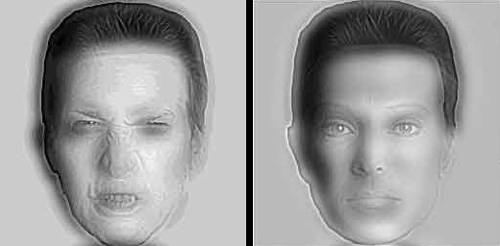
\includegraphics[width=0.96\linewidth]{img/chap4/angrysmile}
	\caption{Stimuli utilisé lors de l'étude de Schyns et Oliva~\cite{schyns-c1999}.}
	\label{fig:angrysmile}
\end{figure}

Cette version de la métrique n'intègre pas encore la gestion des couleurs ou de la localisation spatiale des dégradations. Malgré sa sensibilité aux déformations géométriques comme un décalage spatial ou une rotation, les premiers résultats obtenus sont au même niveau que ceux de SSIM, ce qui encourage les auteurs à poursuivre dans cette voie. Pourtant, l'évaluation pourrait gagner en pertinence en utilisant une base d'images différente de la base LIVE~\cite{sheikh-live} qui n'est pas sans défaut.


\section{Approches basées sur la mesure explicite de dégradations haut niveau}
La qualité visuelle d'une image ou d'une vidéo dépend directement des dégradations visibles qu'elle contient. Celles-ci se définissent comme les causes de la perte de qualité. Nous pouvons les classer en quatre groupes suivant leur origine : la capture, le codage, le transport et l'affichage. Nous ne nous intéressons ici qu'au codage, mais chacune a son importance dans la qualité finale du média concerné.

En fait, l'unique origine des dégradations dues au codage est la quantification réalisée par le codeur. Cependant, elles se manifestent par différents phénomènes visibles, dépendants de nombreux facteurs comme le débit, le contenu ou les paramètres de codage. À haut niveau, elles sont souvent traduites par une liste de dégradations indépendantes comme le flou ou l'effet de bloc~\cite{yuen-sp1998, bretillon-phd, punchihewa-ivcnz2002, crete-phd}. Connaitre a priori le type de dégradation mesurée permet d'exploiter certaines propriétés du média. C'est pourquoi il existe de nombreuses métriques sans référence dans cette catégorie.

Nous commençons ici par proposer un catalogue des dégradations de codage. Puis, nous présenterons un exemple d'étude de la perception des dégradations~\cite{farias-phd}, avant de détailler des mesures et des métriques de qualité basées sur cette approche.

\subsection{Un catalogue de dégradations} \label{ssec:catalogueDeg}
La première étape d'une telle approche est de constituer une liste des dégradations. Cette liste est généralement spécifique à un système dégradant. Nous y distinguons les dégradations spatiales des dégradations temporelles. Ces dernières font l'objet de bien moins d'intérêt que les premières dans la littérature. Voici une liste possible des dégradations spatiales provoquées par le codage :
\begin{description}
\item[Les effets de bloc] \emph{(blockiness)} résultent du traitement par blocs des codeurs comme JPEG et les différentes versions de MPEG. Ils se caractérisent par l'apparition de structures verticales et horizontales plus ou moins régulières, non contenues dans la vidéo ou l'image originale.
\item[L'effet d'ondulation] \emph{(ringing)} résulte d'irrégularités dans la reconstruction des hautes fréquences du bloc reconstruit. Après transformation inverse, des erreurs apparaissent sous forme d'ondulations, particulièrement visible le long des contours fortement contrastés.
\item[Le flou] \emph{(blur)} est provoqué par la suppression des hautes fréquences. Il apparait comme la perte de détails de l'image originale.
\item[Le crénelage] prend habituellement la forme de dentelures et de contours déchirés. Cet effet est le plus important sur des contours proches des directions verticale et horizontale. Le long des diagonales, l'effet est visible mais moins important.
\item[La bavure des couleurs] \emph{(colour bleeding)} est provoquée par une saturation excessive des couleurs. Il se manifeste par le mélange ou la superposition d'une couleur avec une autre au niveau des contours.
\item[Le bruit granulaire] est dû à la quantification des coefficients DCT dans une zone peu détaillée. Avec des valeurs de luminance variant peu d'une image à l'autre, le résultat oscille autour de la valeur à coder. Il apparait comme un fourmillement.
\end{description}

Les dégradations temporelles usuelles sont :
\begin{description} % TODO voir activité de contour = en2fr(edge busyness) avec Domino
\item[Le bruit moustique] \emph{(mosquito noise)} est lié à la différence de codage d'une image à l'autre des informations de la compensation de mouvement soumises à quantification. Il est nommé par comparaison aux battements d'ailes du moustique.
\item[L'activité de contour] \emph{(edge busyness)} se manifeste par une fluctuation autour des contours animés.
\item[L'effet de trainage] \emph{(ghosting effect)} est dû à l'application d'un filtre passe-bas à chaque image prédite afin d'atténuer les détails dans MPEG-2 et de stabiliser l'estimation de mouvement. Il est perçu comme du flou.
% \item scintillement \emph{(flicker)} : provoqué par un faible taux de rafraichissement de l'image ; se manifeste par une discontinuité de la visualisation temporelle des images ;
% \item \emph{judder} : conséquence de la conversion d'un signal vidéo de 24 images par seconde à 29,97 images par seconde, se manifeste par l'apparition de saccades, notamment lors des déplacements latéraux de la caméra ; survient notamment avec les films en haute définition, codés en 24 images par seconde, mais diffusés sur des écrans ou du matériel qui ne supportent que le 60Hz ;
\end{description}

La question de l'exhaustivité d'une telle liste se pose. Jusqu'où aller dans la classification des dégradations ? Celles contenues dans la liste que nous proposons sont les plus classiquement répertoriées dans la littérature~\cite{yuen-sp1998, bretillon-phd}. Cependant, elles sont caractéristiques d'un contexte de codage. Un autre système dégradant pourrait générer une autre liste ou plutôt réduire cette liste. Par ailleurs, toutes les dégradations d'une même liste ne font pas nécessairement l'objet d'une mesure. En fait, alors que le catalogue des dégradations distinguables est assez important, les mesures se limitent généralement à celles ayant le plus d'impact visuel. Il s'agit couramment de l'effet de bloc, du \emph{ringing} et du flou~\cite{farias-phd, crete-phd}. La figure~\ref{fig:artefacts} présente des exemples de ces trois principales dégradations à être considérées dans les mesures de qualité.

\begin{figure}[htbp]
	\centering
	\subfloat[Image originale.]{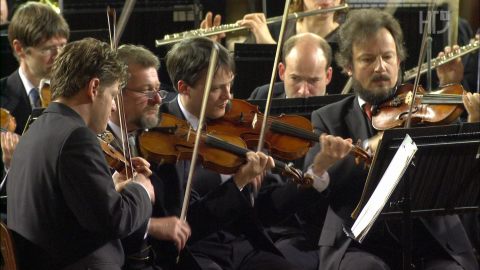
\includegraphics[width=0.43\linewidth]{img/chap4/seqHD}}\hfill
	\subfloat[Image avec effet de bloc.]{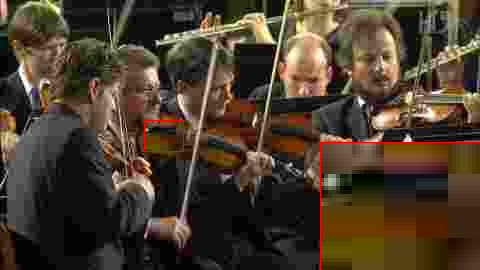
\includegraphics[width=0.43\linewidth]{img/chap4/seqHDbloc}}\\
	\subfloat[Image floue.]{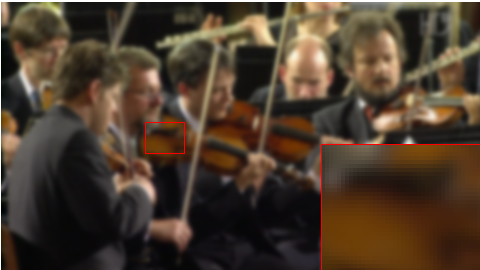
\includegraphics[width=0.43\linewidth]{img/chap4/seqHDflou}}\hfill
	\subfloat[Image avec \emph{ringing}.]{\includegraphics[width=0.43\linewidth]{img/chap4/seqHDjp2}}
	\caption{Illustration sur une image des principales dégradations spatiales prises en compte par les métriques de qualité. Le coin en bas à droite est un agrandissement de la zone entourée de rouge.}
	\label{fig:artefacts}
\end{figure}


\subsection{Un exemple d'étude de la perception des dégradations}
À titre d'exemple d'étude de la perception des dégradations, détaillons cette partie des travaux de thèse de Farias~\cite{farias-phd}. Nous rappelons qu'elle y propose plusieurs expérimentations psychophysiques permettant de modéliser la gêne induite par l'effet de bloc, le flou, le \emph{ringing} et le bruit. Les tâches confiées aux observateurs sont de quatre ordres, parfois même combinés dans une expérimentation :
\begin{itemize}
\item détection d'une ou plusieurs dégradations ;
\item description d'une ou plusieurs dégradations ;
\item mesure de l'intensité d'une ou plusieurs dégradations ;
\item mesure de la gêne due à une ou plusieurs dégradations.
\end{itemize}
%
Les dégradations synthétiques et un codage MPEG-2 sont appliqués à des vidéos de référence par régions isolées. En fonction de l'intensité de la dégradation insérée, l'auteur est capable d'en mesurer l'impact sur les grandeurs évaluées par les observateurs.

Considérons par exemple la première expérimentation qui consiste à détecter et à noter la gêne de l'effet de bloc et du flou. La combinaison des deux dégradations est effectuée de la manière suivante. Pour chaque contenu et chaque zone de dégradation, deux séquences dégradées $S_b$ et $S_n$ sont générées avec les dégradations synthétiques d'effet de bloc et de flou respectivement. Une séquence $S$ utilisée pour l'expérimentation est générée par la moyenne de $S_b$ et $S_n$ :
\begin{equation}
S = \frac{1}{2} \left(S_b + S_n\right).
\end{equation}
%
Cette relation est déterminée à partir de l'observation de la séquence générée. De même, un débit de codage MPEG-2 produisant une combinaison visuellement similaire est déterminé par les auteurs. Cette approche est très discutable dans la mesure où rien n'assure que les vidéos utilisées dans cette étude soient représentatives en termes de contenu et de complexité.

L'auteur utilise cinq séquences vidéos originales, trois zones de dégradation pour chaque séquence et six intensités de dégradations synthétiques ou de débit par zone de dégradation et par vidéo. Cet ensemble de 90 séquences et les cinq vidéos originales sont évalués par 30 observateurs. L'analyse statistique des expérimentations est faite à partir du logarithme de l'erreur quadratique totale, noté $\mathit{LTSE}$ :
\begin{equation}
\mathit{LTSE} = \log\left( \frac{1}{IJK}\sum_i \sum_j\sum_k \left( S'(i,j,t) - S_0(i,j,t) \right)^2\right)
\end{equation}
%
avec $i$, $j$ et $t$ les coordonnées spatio-temporelles des pixels de la séquence dégradée $S'$ et de la séquence d'origine $S_0$ et $I$, $J$ et $K$ les dimensions spatio-temporelles de ces séquences. La détection d'une dégradation conduit à une réponse binaire. La probabilité de détection est calculée en ajustant les données subjectives à une fonction psychométrique de la forme :
\begin{equation}
P(\mathit{LTSE}) = 1 - 2^{-(s_T\cdot \mathit{LTSE})^\kappa}
\end{equation}
%
avec $P$ la probabilité de détection, $s_T$ la sensibilité et $\kappa$ la pente de la fonction. Le seuil de détection est donnée par $\frac{1}{s_T}$. Les MOS, compris en 0 et 100, obtenus lors d'une expérimentation de mesure de la gêne sont nommés MAV \emph{(mean annoyance value)}. La prédiction de la gêne en fonction de l'erreur est effectuée par :
\begin{equation}
A_p(\mathit{LTSE}) = A_{min} + \frac{A_{\textit{max}} - A_{\textit{min}}}{1+\exp\left(-\frac{(\mathit{LTSE}-\mathit{LTSE'})}{\eta}\right)}
\end{equation}
%
avec $A_p$ la gêne prédite par le modèle, $A_{\textit{max}}$ et $A_{\textit{min}}$ les limites de la gamme de valeur de la gêne $A_p$ et $\eta$ la pente de la fonction. La valeur $\mathit{LTSE'}$ correspond à la valeur de la gêne à mi-dynamique $[A_{\textit{min}},A_{\textit{max}}]$.

Les résultats de cette expérimentation sont les suivants. Tout d'abord, les dégradations générées synthétiquement sont visuellement proches des dégradations générées par codage MPEG-2. Elles ont de plus des propriétés de visibilité et de gêne similaires. La figure~\ref{fig:farias} présente le type de fonction obtenu pour une séquence et une zone dégradée. Les fonctions de détection et de gêne pour les dégradations synthétiques et pour un codage MPEG-2 ont la même forme. De plus, les seuils de visibilité sont hautement corrélés avec les valeurs de mi-gêne, ce qui prouve la cohérence de l'expérimentation. La différence la plus notable est que la gêne des dégradations synthétiques est légèrement inférieure à celle des dégradations de codage MPEG-2 pour la même valeur de $\mathit{LTSE}$, ce qui peut s'expliquer par le fait que le codage MPEG-2 introduit une variété de dégradations plus vaste que celle retenue.

\begin{figure}[htbp]
	\centering
	\subfloat[Probabilité de détection en fonction de l'erreur.]{\begin{tikzpicture}% \begin{tikzpicture}
\node at (0,0) {\includegraphics[width=6cm]{img/chap4/farias1}};
% \draw (-3,-2.36) rectangle (3,2.35);

\draw[legende] (-0.2,-0.1) rectangle (2.9,-2.2);

\draw (2.6,-0.4) node[anchor=east,font=\scriptsize] {modèle synthétique};
\draw (2.6,-0.9) node[anchor=east,font=\scriptsize] {données synthétiques};
\draw (2.6,-1.4) node[anchor=east,font=\scriptsize] {modèle MPEG};
\draw (2.6,-1.9) node[anchor=east,font=\scriptsize] {données MPEG};
\fill[blue] (2.6,-0.45) rectangle (2.8,-0.4);
\fill[blue,rotate=135] (-2.525,-1.175) rectangle (-2.575,-1.375);
\fill[blue,rotate=135] (-2.45,-1.25) rectangle (-2.65,-1.3);
\fill[red] (2.6,-1.45) rectangle (2.8,-1.4);
\draw[thick,red] (2.7,-1.92) circle (0.07);

\node[anchor=north] at (-2.8,-2.3) {2,5};
\node[anchor=north] at (-1.65,-2.3) {3};
\node[anchor=north] at (-0.55,-2.3) {3,5};
\node[anchor=north] at (0.6,-2.3) {4};
\node[anchor=north] at (1.7,-2.3) {4,5};
\node[anchor=north] at (2.85,-2.3) {5};
\node[below=0.3cm] at (0,-2.4) {$\mathit{LTSE}$};

\node[anchor=east] at (-2.9,-2.4) {0};
\node[anchor=east] at (-2.9,-1.95) {0,1};
\node[anchor=east] at (-2.9,-1.5) {0,2};
\node[anchor=east] at (-2.9,-1.05) {0,3};
\node[anchor=east] at (-2.9,-0.6) {0,4};
\node[anchor=east] at (-2.9,-0.15) {0,5};
\node[anchor=east] at (-2.9,0.3) {0,6};
\node[anchor=east] at (-2.9,0.75) {0,7};
\node[anchor=east] at (-2.9,1.2) {0,8};
\node[anchor=east] at (-2.9,1.65) {0,9};
\node[anchor=east] at (-2.9,2.1) {1};
\node[rotate=90] at (-3.8,0) {probabilité de détection};

% \end{tikzpicture}\end{tikzpicture}}\hfill
	\subfloat[Gêne moyenne en fonction de l'erreur.]{\begin{tikzpicture}% \begin{tikzpicture}
\node at (0,0) {\includegraphics[width=6cm]{img/chap4/farias2}};
% \draw (-3,-2.36) rectangle (3,2.35);

\def\shiftX{-2.5}
\def\shiftY{2}

\draw[legende] (-0.2+\shiftX,-0.1+\shiftY) rectangle (2.9+\shiftX,-2.2+\shiftY);
\draw (2.6+\shiftX,-0.4+\shiftY) node[anchor=east,font=\scriptsize] {modèle synthétique};
\draw (2.6+\shiftX,-0.9+\shiftY) node[anchor=east,font=\scriptsize] {données synthétiques};
\draw (2.6+\shiftX,-1.4+\shiftY) node[anchor=east,font=\scriptsize] {modèle MPEG};
\draw (2.6+\shiftX,-1.9+\shiftY) node[anchor=east,font=\scriptsize] {données MPEG};
\fill[blue] (2.6+\shiftX,-0.45+\shiftY) rectangle (2.8+\shiftX,-0.4+\shiftY);
\fill[blue,rotate=135] (0.675,-0.825) rectangle (0.625,-1.025);
\fill[blue,rotate=135] (0.75,-0.9) rectangle (0.55,-0.95);
% \fill[blue,rotate=135] (-2.525,-1.175) rectangle (-2.575,-1.375);
% \fill[blue,rotate=135] (-2.45,-1.25) rectangle (-2.65,-1.3);
\fill[red] (2.6+\shiftX,-1.45+\shiftY) rectangle (2.8+\shiftX,-1.4+\shiftY);
\draw[thick,red] (2.7+\shiftX,-1.92+\shiftY) circle (0.07);

\node[anchor=north] at (-1.8,-2.3) {3};
\node[anchor=north] at (-0.55,-2.3) {3,5};
\node[anchor=north] at (0.65,-2.3) {4};
\node[anchor=north] at (1.85,-2.3) {4,5};
\node[below=0.3cm] at (0,-2.4) {$\mathit{LTSE}$};

\node[anchor=east] at (-2.9,-2.35) {0};
\node[anchor=east] at (-2.9,-1.9) {10};
\node[anchor=east] at (-2.9,-1.45) {20};
\node[anchor=east] at (-2.9,-1.05) {30};
\node[anchor=east] at (-2.9,-0.55) {40};
\node[anchor=east] at (-2.9,-0.1) {50};
\node[anchor=east] at (-2.9,0.45) {60};
\node[anchor=east] at (-2.9,0.85) {70};
\node[anchor=east] at (-2.9,1.4) {80};
\node[anchor=east] at (-2.9,1.85) {90};
\node[anchor=east] at (-2.9,2.3) {100};
\node[rotate=90] at (-3.8,0) {gêne moyenne};


% \end{tikzpicture}
\end{tikzpicture}}
	\caption{Exemple de résultats obtenu par Farias~\cite{farias-phd}.}
	\label{fig:farias}
\end{figure}

Une telle étude permet de déterminer des fonctions de gêne très intéressantes pour déterminer l'impact des dégradations de codage sur la perception de la qualité. Comme nous l'avons déjà mentionné, la principale limitation de ce type d'approche est la difficulté des tâches demandées aux observateurs. Une telle complexité peut modifier ou biaiser les mesures subjectives sur lesquelles il est difficile de construire des modèles pertinents et fiables.


\subsection{Mesures de dégradations}
\subsubsection{Mesure de l'effet de bloc}
L'effet de bloc étant courant avec les systèmes de codage à base de transformation DCT, de nombreuses mesures dédiées ont vu le jour~\cite{karunasekera-spie1993,coudoux-jvcir1997}. De plus, l'origine de la dégradation étant bien connue, il est pratique de l'exploiter pour effectuer la mesure. C'est pourquoi des critères sans référence sont possibles~\cite{perra-icip2005,liu-measureReducBlock,meesters-sp2002, babu-pv2004}. Il existe beaucoup plus de méthodes pour images fixes que pour la vidéo. Leontaris~\cite{leontaris-icassp2005} en a évaluer plusieurs dont la plupart étaient pour images fixes. Il a mesuré leurs performances image par image et, pour la vidéo, considère la moyenne temporelle, ce qui ne semble pas les désavantager significativement par rapport à celles conçues pour la vidéo.

Les techniques de mesure peuvent être classées selon le domaine considéré pour le calcul : domaine spatial ou domaine fréquentiel. Le premier groupe contient les mesures utilisant le domaine des fréquences spatiales~\cite{gao-tcsvt2002}. Ils exploitent le fait que les frontières de bloc sont spatialement régulières et forment donc des pics de fréquences. Par exemple, Farias~\cite{farias-phd} en propose une basée sur celle pour images fixes de Wang~\cite{wang-icip2000}. Celle-ci modélise l'image dégradée par la somme de l'image d'origine et d'un signal de pur effet de bloc. La méthode calcule d'abord les gradients horizontaux et verticaux de l'image originale. Elle applique ensuite une FFT \emph{(Fast Fourier transform)} unidimensionnelle. La mesure globale de l'effet de bloc est estimée comme la différence entre les puissances spectrales des deux images. La méthode intègre également les effets de masquage dus au contenu de l'image. Elle considère ainsi qu'un effet de bloc est moins visible dans une zone de texture que dans une zone sans texture.

Le second groupe de mesures utilisent le domaine spatial~\cite{pan-iscs2004,wang-icip2002}. Celles-ci estiment l'effet de bloc en détectant les contours non naturels correspondant à la dégradation. Par exemple, Vlachos~\cite{vlachos-detection} propose un critère basé sur la corrélation entre des sous-images de l'image originale. En tout, huit sous-images sont créées. Chacune est constituée des pixels de l'image originale situés à une position donnée dans un bloc 8\texttimes8. Ceci est illustré sur la figure~\ref{fig:vlachos}. La sous-image $s(0,1)$ contient ainsi les pixels indiqués par un point. Les quatre sous-images utilisées pour la corrélation inter-bloc sont $s_1=s(7,7)$, $s_2=s(0,7)$, $s_3=s(7,1)$ et $s_4=s(0,1)$. Les quatre sous-images utilisées pour la corrélation intra-bloc sont $s_5=s_4=s(0,1)$, $s_6=s(1,3)$, $s_7=s(0,3)$ et $s_8=s(3,3)$ car dans le cas d'une séquence entrelacée, les pixels d'une sous-image appartiennent à une même trame. %Le résultat des corrélations sont des surfaces dont seules les valeurs maximales sont retenues pour la suite. La mesure de l'effet de bloc $B$ est calculée comme le rapport entre la somme des valeurs maximales des corrélations inter-bloc $C_r$ et la somme des valeurs maximales des corrélations intra-bloc $C_a$ :
La mesure de l'effet de bloc $M_B$ est calculée comme le rapport entre la corrélation inter-bloc $C_r$ et la corrélation intra-bloc $C_a$ :
\begin{equation}
M_B = \frac{\sum\limits_{i=6}^8 C_r(s_5, s_i)}{\sum\limits_{i=2}^4 C_a(s_1,s_i)}.
\end{equation}
%
Dans une image avec peu d'effet de bloc, ce rapport sera proche de l'unité, alors qu'il sera significativement supérieur en présence d'effet de bloc. Ce type de méthode a l'avantage de savoir exactement où sont situés les dégradations si le codeur utilise un découpage en bloc régulier. Par contre, la mesure est perturbée par le contenu de l'image ou la vidéo qui se superpose aux effets de bloc.

\begin{figure}[htbp]
  \centering
  \begin{tikzpicture}[scale=0.4]% \begin{tikzpicture}

\foreach \y in {0,1,2,3,4,5,6,7,9,10,11,12,13,14,15,16} {
	\foreach \x in {0,1,2,3,4,5,6,7,9,10,11,12,13,14,15,16} {
		\draw (\x,\y) -- (\x+0.8,\y) -- (\x+0.8,\y+0.8) -- (\x,\y+0.8) -- cycle;
	}
}

\draw[dashed] (8.4,-0.2) -- (8.4,17);
\draw[dashed] (-0.2,8.4) -- (17,8.4);

\draw (0.4,6.35) node{$\bullet$};
\draw (9.4,6.35) node{$\bullet$};
\draw (0.4,15.35) node{$\bullet$};
\draw (9.4,15.35) node{$\bullet$};

\draw (0.4,0.35) node{$\blacksquare$}; % $\blacksquare$
\draw (9.4,0.35) node{$\blacksquare$};
\draw (0.4,9.35) node{$\blacksquare$};
\draw (9.4,9.35) node{$\blacksquare$};

\draw (7.4,0.35) node{$\bigstar$}; % \bigstar
\draw (16.4,0.35) node{$\bigstar$};
\draw (7.4,9.35) node{$\bigstar$};
\draw (16.4,9.35) node{$\bigstar$};

\draw (7.4,6.35) node{$\blacktriangledown$}; % \blacktriangledown
\draw (16.4,6.35) node{$\blacktriangledown$};
\draw (7.4,15.35) node{$\blacktriangledown$};
\draw (16.4,15.35) node{$\blacktriangledown$};

% \end{tikzpicture}
\end{tikzpicture}
  \caption{Pixels considérés dans les sous-images de la mesure de l'effet de bloc de Vlachos. Cas d'une image entrelacée.}
  \label{fig:vlachos}
\end{figure}

Ces mesures exploitent une propriété connue des systèmes de codage utilisant un découpage par blocs. Cependant, même pour un tel codage, Crete~\cite{crete-phd} a montré que s'appuyer sur la périodicité de l'effet pouvait être risqué, notamment dans les cas à fort taux de compression. Elle définit le phénomène de bloc étendu comme la diminution du nombre de frontières artificielles dues au codage. Cela provoque l'apparition de frontières très visibles délimitant des zones homogènes où les frontières entre blocs sont invisibles. Ce phénomène est illustré sur la figure~\ref{fig:blocEtendu}. Une métrique qui associe un poids à chaque frontière et qui construit sa note finale en fonction de ces poids attribuera une valeur nulle à ces frontières invisibles. La note finale sera ainsi diminuer pour les fortes compressions, alors que ces frontières n'ont pas d'impact perceptuel. Seules quelques mesures prennent en compte ce phénomène~\cite{gao-tcsvt2002,pan-iscs2004}.

\begin{figure}[htbp]
  \centering
  \includegraphics[width=0.8\linewidth]{img/chap4/blocEtendu}
  \caption{Illustration du phénomène de bloc étendu. Le coin en haut à droite est un agrandissement de la zone entourée de noir. Photo \href{http://www.sxc.hu/photo/946616}{www.sxc.hu}.}
  \label{fig:blocEtendu}
\end{figure}


\subsubsection{Mesure du flou} \label{ssec:flou}
Le principe usuel de la mesure du flou est d'évaluer les pertes en hautes fréquences via la variation de l'étalement des contours. À l'heure actuelle, il en existe bien moins que de mesures de l'effet de bloc dans la littérature~\cite{elder-pami1998,wu-icsp2005,hu-icip2006}.

Celle de Marziliano~\cite{marziliano-blurmetric} est de type sans référence. Elle détecte les contours verticaux sur la composante de luminance par un filtre de Sobel. L'auteur considère en effet comme suffisant de ne mesurer le flou que sur les contours verticaux. L'image est ensuite parcourue horizontalement, c'est-à-dire dans la direction normale aux contours. Les origines et les terminaisons des contours sont détectées à partir des valeurs minimales et maximales locales de la ligne considérée. La figure~\ref{fig:marzi} présente le profil d'une ligne d'une image. Les contours détectés sont indiqués par les lignes en tirets. Les valeurs minimales et maximales locales sont indiquées par les lignes en pointillés. La largeur du contour est calculée par la différence entre son origine et sa terminaison. Elle correspond à la mesure locale du flou pour ce contour. La mesure globale de flou de l'image est calculée en moyennant les mesures locales de tous les contours  détectés. Cette technique a l'avantage d'être très intuitive. Cependant dans le cas du codage, elle va être perturbée par d'autres dégradations comme l'effet de bloc qui va créer des contours artificiels.

\begin{figure}[htbp]
  \centering
  \begin{tikzpicture}[xscale=0.258,yscale=0.0325]
\draw (140,0) rectangle (180,250);
\draw[very thick] (140,150) -- (142,158) -- (143,148) -- (144,152) -- (145,168) -- (146,190) -- (148,197) -- (149,197) -- (150,188) -- (151,168) -- (153,130) -- (154,119) -- (155,116) -- (156,116) -- (157,114) -- (158,111) -- (159,111) -- (160,115) -- (161,117) -- (162,117) -- (163,113) -- (165,92) -- (166,90) -- (169,64) -- (171,41) -- (172,47) -- (176,200) -- (177,220) -- (178,216) -- (179,216) -- (180,215);
\draw[yscale=7.9385] (142,19.8) circle (0.3);
\draw[dotted] (142,0) -- (142,158);
\draw[yscale=7.9385] (143.05,18.6) circle (0.3);
\draw[dotted] (143,0) -- (143,148);
\draw[yscale=7.9385] (144,19.1) circle (0.3);
\draw[loosely dashed,thick] (144,0) -- (144,152);
\draw[yscale=7.9385] (148.05,24.9) circle (0.3);
\draw[dotted] (148,0) -- (148,197);
\draw[yscale=7.9385] (151.05,21.2) circle (0.3);
\draw[loosely dashed,thick] (151,0) -- (151,168);
\draw[yscale=7.9385] (159.05,14) circle (0.3);
\draw[dotted] (159,0) -- (159,111);
\draw[yscale=7.9385] (161,14.8) circle (0.3);
\draw[dotted] (161,0) -- (161,117);
\draw[yscale=7.9385] (167,10.4) circle (0.3);
\draw[loosely dashed,thick] (167,0) -- (167,85);
\draw[yscale=7.9385] (171,5.34) circle (0.3);
\draw[dotted] (171,0) -- (171,41);
\draw[yscale=7.9385] (174,15.2) circle (0.3);
\draw[loosely dashed,thick] (174,0) -- (174,120);
\draw[yscale=7.9385] (177,27.8) circle (0.3);
\draw[dotted] (177,0) -- (177,220);
\draw[yscale=7.9385] (178,27.2) circle (0.3);
\draw[dotted] (178,0) -- (178,216);
\draw[yscale=7.9385] (179,27.2) circle (0.3);
\draw[dotted] (179,0) -- (179,216);

\foreach \x in {140,150,160,170,180} \draw (\x,1) -- (\x,-1) node[anchor=north] {\x};
\foreach \y in {0,50,100,150,200,250} \draw (139.75,\y) -- (140.25,\y) node[anchor=east] {\y};
\node at(160,-20) {Position};
\node[rotate=90] at(137,125) {Niveau de gris};
\end{tikzpicture}
  \caption{Profil d'une ligne d'une image et points utilisés pour la mesure du flou~\cite{marziliano-blurmetric}.}
  \label{fig:marzi}
\end{figure}


\subsubsection{Mesure du \emph{ringing}}
Comme pour le flou, il existe peu de mesures du \emph{ringing}~\cite{feng-spie2006}. Suite à ses travaux sur le flou, Marziliano~\cite{marziliano-ringingmetric} s'y est intéressée, particulièrement dans le cadre de JPEG2000. Sa mesure de \emph{ringing} utilise d'ailleurs celle de flou. En parcourant chaque ligne de l'image, le défaut est mesuré le long de chaque contour. Deux mesures sont alors définies, l'une à gauche du contour, l'autre à droite. Le support total du \emph{ringing} est définit comme la différence entre une largeur constante d'oscillation du \emph{ringing} et la largeur du contour calculée par la mesure de flou. La largeur constante d'oscillation est un a priori sur les effets de la décomposition en ondelettes utilisée dans JPEG2000. La différence entre le minimum et le maximum de l'image de différence est multipliée par la taille de ce support de \emph{ringing}. La mesure de \emph{ringing} du contour est égale à la moyenne entre la valeur de la mesure de gauche et celle de droite. La mesure globale de \emph{ringing} de l'image est calculée en moyennant les mesures locales de tous les contours détectés.

Cette technique souffre évidemment des mêmes défauts que celle de flou. Elle utilise de plus une hypothèse sur la valeur de la largeur d'oscillation spécifique au codage JPEG2000. Cela rend sa mesure extrêmement spécifique à ce système dégradant et en réduit d'autant l'utilisabilité. Elle est cependant l'une des rares mesures de ce défaut.


\subsection{Métriques de qualité}
Certaines études vont plus loin que la mesure de dégradations. À partir d'une ou plusieurs de ces mesures, elles construisent une métrique de qualité. %Nous les classons suivant le nombre de dégradation qu'elles considèrent.


\subsubsection{Métriques basées sur une seule dégradation}
Seule Marziliano a utilisé une unique mesure de dégradations pour prédire la qualité subjective d'images fixes. Elle a évalué les performances de sa mesure de flou par des tests subjectifs réalisés par dix experts avec cinq images fixes originales~\cite{marziliano-blurmetric}. Celles-ci sont dégradées soit synthétiquement par un filtre gaussien, soit par un codeur JPEG2000. Cinq dégradations de chaque type sont appliqués sur chaque image. Le coefficient de corrélation entre les notes subjectives et les mesures calculées est de 0,96 pour les images dégradées par le filtrage gaussien et de 0,85 pour les images dégradées par JPEG2000. Les bonnes performances avec le filtre gaussien ne sont pas surprenantes car la mesure y est bien adapté, de par son principe. La faible valeur obtenue avec JPEG2000 s'explique par le fait que cette compression n'engendre pas seulement du flou mais aussi d'autres dégradations, dont du \emph{ringing}.

Elle évalue également sa métrique de \emph{ringing}~\cite{marziliano-ringingmetric}. Des tests subjectifs sont réalisés avec neuf images originales et cinq qualités JPEG2000. Le coefficient de corrélation entre les mesures subjectives et les notes objectives est de 0,85. L'auteur explique cette faible valeur par le fait qu'il est difficile pour les observateurs d'évaluer le \emph{ringing} seul dans les images JPEG2000. Ceci montre la difficulté de réaliser des tests psychophysiques demandant aux observateurs de ne se focaliser que sur un unique type de dégradations alors que d'autres sont simultanément présents.


\subsubsection{Métriques basées sur plusieurs dégradations}
Baser une métrique de qualité sur plusieurs mesures de dégradations pose le problème de leur cumul. Les modèles utilisés par la majorité des métriques sont souvent simples. Par exemple, Wang combine une mesure de flou et une d'effet de bloc~\cite{wang-icip2002}. Ces deux mesures sont issues de sa mesure d'effet de bloc~\cite{wang-icip2000}. Le flou est alors estimé par le décalage d'énergie des hautes fréquences vers les basses fréquences. Trois caractéristiques sont calculées avant de générer la note de qualité finale. Chacune est mesurée verticalement et horizontalement, la moyenne des deux mesures étant considérée dans la suite. La première caractéristique est la mesure de l'effet de bloc $b_W$. La seconde est dérivée de la mesure de flou et de celle d'effet de bloc, les auteurs la nomment mesure d'activité $a_W$. La dernière est issue du calcul des gradients vertical et horizontal. Les compteurs $z_h$ et $z_v$ sont incrémentés à chaque fois que les gradients horizontal et vertical s'annulent respectivement. La caractéristique $z_W$ est égale à la moyenne de ces compteurs divisée par le nombre de valeurs du gradient. Enfin, la note de qualité est donnée par le modèle :
\begin{equation}
M_W = \alpha + \beta\cdot b_W^{\gamma_1}\cdot a_W^{\gamma_2}\cdot z_W^{\gamma_3}
\end{equation}
%
avec $\alpha$, $\beta$, $\gamma_1$, $\gamma_2$ et $\gamma_3$ les paramètres à optimiser. Cette optimisation est obtenue à partir de données subjectives, c'est-à-dire que les valeurs retenues sont celles minimisant l'erreur de prédiction de MOS connus. Le danger de ce type d'approche est le sur-entrainement du modèle. Si les données manquent de variété, par exemple dans la gamme d'activité des images, les paramètres ne s'adapteront pas à des conditions différentes et le modèle manquera de robustesse.

Farias~\cite{farias-phd} propose un critère de qualité intégrant à la fois une mesure d'effet de bloc $b_F$, une de flou $f_F$ et une de bruit $n_F$. Les mesures utilisées sont adaptées de mesures existantes dans la littérature comme celle de Vlachos~\cite{vlachos-detection} pour l'effet de bloc et celle de Marziliano~\cite{marziliano-blurmetric, marziliano-ringingmetric} pour le flou. Le modèle de cumul final utilise une sommation de Minkowski :
\begin{equation}
M_F = \left( w_b\cdot b_F^p + w_f\cdot f_F^p + w_n\cdot n_F^p \right)^{\frac{1}{p}}
\end{equation}
%
avec $\beta$ l'exposant de la sommation et $w_b$, $w_f$ et $w_n$ les pondérations des mesures $b_F$, $f_F$ et $n_F$ respectivement. Ces pondérations peuvent être nulles, si l'une ou plusieurs des mesures ne sont pas prises en compte. Le cumul adopté est donc très simple. Cela est regrettable compte tenu de la nature de l'étude. Elle consistait en effet à mesurer à la fois la gêne induite par chaque dégradation, par leurs combinaisons et par un système dégradant de type MPEG-2. Cela aurait pu mener à un modèle de cumul plus évolué car bâtit sur des résultats psychovisuels individuels, combinés et comparés à des dégradations réelles.

Caviedes~\cite{caviedes-nrqm} a une approche similaire mais en plus de mesures de dégradations liées au codage, il intègre des mesures de contraste et de netteté. Au final, il combine six mesures : $b_C$ pour l'effet de bloc ; $r_C$ pour le \emph{ringing} ; $c_C$ pour le \emph{clipping}, dégradation due à la troncation de bits imposée par la précision des calculs ; $n_C$ pour le bruit ; $o_C$ pour le contraste et enfin $s_C$ pour la netteté. La méthode de détermination du cumul est la suivante. Les auteurs disposent d'un ensemble de séquences d'entrainement, dont ils connaissent les mesures subjectives et les six notes objectives. Plutôt que de chercher une solution de manière exhaustive, les auteurs adoptent une approche incrémentale. Les mesures sont ajoutées et évaluées au fur et à mesure. Cela permet à la fois de limiter les calculs mais aussi d'évaluer l'apport de chaque contribution en termes d'impact sur la qualité subjective. Dans un premier temps, les six mesures principales sont calculées. La seconde étape fournit les interactions entre certaines de ces mesures. Finalement, la mesure de qualité NROQM \emph{(No-reference objective quality metric)} est obtenue par la formule :
\begin{equation}
\begin{array}{rl}
M_C =	& - \frac{1}{\gamma_3}\left(1+o_C + \frac{n_C}{\gamma_1}\right)\left( b_C^{\gamma_2} + \frac{b_C}{1+b_C}r_C^{\gamma_2} \right) - (1+ o_C)(1+\gamma_4\times c_C)^{\gamma_5}\\
			& - \gamma_6n_Cs_Co_C - \frac{1}{\left( 1+\gamma_4c_C\right)^{\gamma_7}}\left( \frac{n_C}{o_C}\right)^{\gamma_8} - \left( \gamma_9+\gamma_{10}o_C\right)^{\gamma_{11}} + s_C
\end{array}
\end{equation}
%
avec $\gamma_i ; i \in [1 ; 11]$ les paramètres du modèle. Plus évolué, celui-ci montre bien la complexité à laquelle le cumul de différentes mesures peut mener. L'approche incrémentale adoptée est originale. Elle permet de ne pas considérer toutes les mesures en un bloc, mais de les ajouter au modèle une par une. La question qui se pose néanmoins est de savoir si l'ordre adopté pour ajouter ces mesures a une influence sur le modèle de cumul obtenu.


\section{Discussion}
\subsection{Sur la diversité des approches}
Dans ce chapitre, nous avons présenté quelques critères de qualité afin d'appréhender les diverses approches existant dans la littérature. Ce panorama montre la richesse et le dynamisme du domaine de l'évaluation objective de la qualité de l'image et de la vidéo. Cela n'est pas surprenant devant l'importance actuelle de ces médias numériques.

L'approche purement signal est la plus utilisée par le domaine du codage alors que c'est celle qui propose le moins de critères. Pourtant, nous pouvons nous interroger sur la prise de conscience de ses limites et de son bon usage. Lorsque la demande en robustesse s'accroit, les utilisateurs de critères de qualité sont alors demandeurs de critères précis, robustes et si possible, capables d'évaluer une séquence en temps-réel. Reconnaissons tout de même que peu de critères existants remplissent ces conditions.

Les critères basés sur la modélisation bas niveau du système visuel humain sont intéressants car ils sont proches du phénomène réel de la vision humaine. Cette proximité leur permet d'être génériques, car ils ne dépendent ni d'un système dégradant, ni d'un système d'affichage, ni d'un mode de transmission. Les études engagées dans cette voie permettent parallèlement d'acquérir une connaissance accrue sur le mode de fonctionnement bas niveau de l'observateur humain. Les applications de telles connaissances sont larges et vont bien au-delà de l'évaluation de la qualité d'image ou de la vidéo. Cependant dans le contexte de l'évaluation de la qualité vidéo, la modélisation des phénomènes bas niveau ne suffit pas. L'absence de prise en compte des aspects haut niveau restreint fortement les performances. De plus, ces critères sont souvent complexes à mettre en \oe uvre et à expliquer aux ingénieurs désireux d'en appréhender l'usage.

Les approches basées sur la fidélité structurelle permettent de considérer certains aspects de plus haut niveau. La simplicité des calculs mis en jeu facilite le traitement, l'analyse et l'optimisation des algorithmes. Cependant, le paradigme structurel de l'image, tel qu'il est posé en hypothèse, est discutable. Aucune définition de cette structure n'est usuellement admise. Rien n'assure que les dégradations de la structure mesurées par ces critères correspondent à une réalité perceptuelle.

Enfin, les approches basées sur la mesure explicite de dégradations haut niveau sont étroitement liés aux systèmes dégradants existants. La principale limite de l'approche vient de la difficulté d'isoler les effets d'une dégradation donnée. Une liste de dégradations ne correspond pas à des effets isolés appliqués successivement, mais à un processus complexe où les dégradations se superposent les unes aux autres dans l'espace et dans le temps. Cette technique rend également délicate l'évaluation subjective des dégradations, car il est difficile pour l'observateur de les isoler.


\subsection{Sur les performances}
Nous l'avons vu, il difficile de comparer une telle diversité d'approches ou même certains critères existants. VQEG est le groupe d'experts chargé de cette tâche. En plus de 10 ans d'existence, il a publié deux études comparatives sur les critères d'évaluation de la télévision avec référence complète~\cite{vqeg-frtv1,vqeg-frtv2}. Les travaux actuels portent sur l'évaluation de la télévision avec référence réduite ou sans référence, du multimédia et de la télévision haute définition. Le plan de tests portant sur le multimédia~\cite{vqeg-MMtestplan} est sur le point d'être achevé. Pour comprendre le considérable effort que cela représente, signalons que ce plan prévoit l'étude avec trois résolutions d'affichage, 14 tests par résolutions et 136 vidéos par test. Ces tests sont réalisés par de nombreux laboratoires de par le monde, pour un total dépassant 5000 vidéos évaluées.

La première campagne a notamment montré que les critères basés sur la modélisation bas niveau du système visuel humain n'obtiennent pas de performances significativement supérieures à celles du PSNR. Lors de la seconde campagne d'évaluation, deux tests distincts ont été réalisés. Le premier utilisait des séquences au format PAL de 625 lignes, le second des séquences au format NTSC de 525 lignes. Les résultats de l'étude sur les deux tests sont proches, sans être cependant identiques. En général, les critères obtiennent des performances différentes sur les deux tests. Le meilleur coefficient de corrélation, obtenu par VQM~\cite{wolf-vqmtech}, est de 0,938 sur les séquences NTSC. Le même critère n'obtient plus que 0,886 sur l'autre test. Métrique un peu particulière car combinant des aspects signal et perceptuel, VQM sera plus particulièrement détaillée dans le chapitre suivant. La différence de performance est sensible, alors que les deux jeux de séquences ne sont pas très différents. Il semble donc difficile de réaliser un critère robuste qui fonctionnerait bien dans des configurations différentes. La quête du critère unique à usage multiple est semble-t-il vaine, tant la diversité des conditions d'utilisation est grande.

Les approches basées sur la mesure explicite de dégradations haut niveau obtiennent de bonnes performances sur des images dégradées synthétiquement. Cependant, ces performances chutent fortement dans des conditions réelles de codage. Ainsi, les utiliser individuellement pour considérer la qualité n'est pas envisageable. En combiner plusieurs soulève le problème de leur combinaison. %En outre, considérer une liste de dégradations haut niveau ne permet pas d'atteindre l'origine réelle de toutes ces dégradations : l'erreur de quantification.


\subsection{Sur les cumuls}
Tout critère se trouve confronté au problème du cumul des grandeurs locales en une note de qualité finale. Pourtant, nous avons constaté que cet aspect était rarement approfondi par les critères de qualité d'image et de vidéo. Ce cumul est souvent réduit à une sommation de Minkowski qui ne prend pas en compte tous les aspects des grandeurs à fusionner. Or, nous considérons qu'il revêt une grande importance dans la structure globale d'un critère de qualité. En effet, il correspond à l'élaboration finale de la note de qualité. C'est là que l'observateur fusionne l'ensemble des erreurs qu'il a perçu en une évaluation quantitative de la qualité de la séquence.

Nous distinguons trois intégrations majeures : sur les grandeurs locales, sur l'espace et sur le temps. Suivant l'approche adoptée, la nature des grandeurs locales varie. Si le critère décompose la vidéo en composantes perceptuelles, il faudra fusionner les fréquences. S'il utilise des caractéristiques calculés dans des blocs, il faudra fusionner ces caractéristiques. La figure~\ref{fig:figCumul} présente un exemple d'enchainement de ces intégrations.

\begin{figure}[htbp]
	\centering
	\begin{tikzpicture}[text centered, node distance = 3cm]% \begin{tikzpicture}[text centered]
% Place nodes
	\node[text width=2cm] (info) {grandeurs locales};
	\node[action, right of=info, text width=2cm] (cumul) {cumul sur les grandeurs};
	\node[action, right of=cumul] (spatial) {cumul spatial};
	\node[action, right of=spatial,text width=2cm] (temp) {cumul temporel};
	\node[right of=temp] (note) {note finale};

% Draw edges
	\path[fleche] (info) -- (cumul);
	\path[fleche] (cumul) -- (spatial);
	\path[fleche] (spatial) -- (temp);
	\path[fleche] (temp) -- (note);
% \end{tikzpicture}\end{tikzpicture}
	\caption{Exemple d'enchainement des cumuls à effectuer pour fusionner les grandeurs locales en une note de qualité finale.}
	\label{fig:figCumul}
\end{figure}

L'ordre utilisé sur cette figure n'est qu'un exemple. En fait, la manière dont les différents cumuls s'enchainent est une question à laquelle peu de travaux se sont intéressés. Citons le cas du cumul fréquentiel, pour lequel Bekkat~\cite{bekkat-phd} a montré que l'ordre entre le cumul angulaire et le cumul radial n'était pas un élément sensible. D'après Le Callet~\cite{lecallet-phd}, il faut systématiquement effectuer le cumul fréquentiel avant le cumul spatial car cet ordre traduit la stratégie du système visuel humain à percevoir les dégradations d’abord localement, puis à regrouper l’ensemble des dégradations perçues sur tous les sites de l’image.

Au final, la méthode de cumul idéale n'est pas encore bien connue. Mettant en jeu des comportements haut niveau du système visuel humain, la construction du jugement à partir de mesures locales nécessite encore un approfondissement certain. En particulier, le passage de l'évaluation de qualité de l'image à celle de la vidéo est un point sensible du problème, spécifique aux critères de qualité vidéo. En effet, utiliser un critère pour image fixe et considérer que la mesure de qualité de la séquence est la moyenne des mesures de qualité des images de la séquence est particulièrement inefficace. Les interactions espace-temps ont donc un impact non négligeable dans la construction du jugement. Pourtant, il existe encore peu d'études sur ce point précis dans la littérature.


\section{Conclusion}
Dans ce chapitre, nous avons réalisé une vue d'ensemble des approches existantes en termes de critères objectifs de la qualité vidéo. Nous avons classé les grands courants de recherche actuels en quatre familles principales : l'approche purement signal ; les approches basées sur la modélisation de la vision humaine bas niveau ; les approches basées sur la fidélité structurelle ; les approches basées sur la mesure explicite de dégradations haut niveau.

L'approche purement signal consiste à utiliser des outils basiques considérant les différences pixel à pixel entre séquences. Bien que très répandues et utilisables dans des conditions particulières, ces métriques ne sont pas assez robustes dans leur prédiction de la qualité vidéo. Les approches basées sur la modélisation de la vision humaine bas niveau sont plus évoluées et plus complexes. Malgré leur capacité à mesurer des phénomènes locaux, elles ne prennent assez en considération les aspects haut niveau du système visuel humain pour réussir à en reproduire fidèlement le comportement. Tentant de prendre en compte certains de ces aspects haut niveau, les approches basées sur la fidélité structurelle ont montré de bonnes performances sur certains ensembles de séquences. Cependant, les métriques proposées ont l'inconvénient de générer une prédiction très sensible aux facteurs intervenant dans leur calcul. De plus, la définition même de la structure d'une image ou d'une vidéo reste à établir clairement. Enfin, les approches basées sur la mesure explicite de dégradations haut niveau considèrent les impacts du codage tels que l'effet de bloc ou le flou. Cependant, mesurer ces effets individuellement n'a pas beaucoup de sens dans la mesure où le codage est un phénomène complexe où les dégradations sont inter-dépendantes. Les individualiser est une approche périlleuse, autant pour leur notation objective que pour leur évaluation subjective. Les travaux de Farias~\cite{farias-phd} ont de plus montré que cette approche n'est pas toujours robuste sur des contenus différents.

Les multiples approches proposées n'ont donc pas apporté, loin s'en faut, toutes les solutions à la problématique de l'évaluation objective de la qualité. Notamment, la problématique du cumul des grandeurs locales en une note de qualité finale n'est pas encore bien caractérisée et souvent sous-estimée. De plus, le cadre spécifique de la télévision haute définition, dont nous avons montré les différences significatives avec la télévision standard, n'est pas traité. VQEG prépare actuellement son plan de test adapté à ce contexte~\cite{vqeg-hdtvtestplan}. Comment les métriques existantes s'y comporterait-elles ? C'est l'une des questions auxquelles le chapitre suivant tente d'apporter une réponse.


\ornementChapitre

% %%%%%%%%%%%%%%%%%%%%%%%%%%%%%%%%%%%%%%%%%%%%%%%%%
%%%
%%% Auteur : Stéphane Péchard - stephane.pechard@univ-nantes.fr
%%% Fichier : 5-eval.tex - chapitre 5 :  Évaluation de critères sur une base de séquences haute définition (15 pages)
%%% Version : 0.1
%%% Date : 2008/02/12
%%%
%%%%%%%%%%%%%%%%%%%%%%%%%%%%%%%%%%%%%%%%%%%%%%%%%
\chapter{Performances de critères objectifs de qualité visuelle en télévision haute définition} \label{chap:evalCrit}
\opt{final}{\lettrine[lines=4]{U}{n critère objectif de qualité visuelle}}\opt{nofinal}{Un critère objectif de qualité visuelle} doit produire une grandeur reflétant autant que possible le jugement humain. Mesurer la fidélité du critère objectif à ce jugement humain revient à évaluer le critère correspondant. La question de l'évaluation des critères est cruciale. En effet, elle permet d'une part de connaitre les performances d'un critère vis-à-vis du jugement subjectif, et d'autre part de disposer d'indicateurs permettant la comparaison des critères objectifs entre eux. Pourtant, il est rare que les auteurs de critères objectifs fournissent un ensemble complet de tels indicateurs de performance. Nous cherchons donc ici à nous doter de mesures de performance mais également de moyens de distinguer si les mesures obtenues par deux critères sont significativement différentes ou pas.

Une fois ces outils définis, nous proposons de les mettre en application. Nous avons constaté qu'aucun critère de qualité vidéo n'était spécialisé dans l'évaluation de la qualité de la TVHD. Bien que nous ayons montré des différences sensibles entre la TVHD et la TVSD, peut-être que des critères existants peuvent prédire de manière efficace la qualité visuelle de la TVHD. Nous devons donc savoir comment des critères performants en TVSD s'adaptent à ce contexte différent. Ainsi, nous avons évalué deux critères de qualité vidéo avec référence complète sur une base de séquences de télévision haute définition. Pour cela, nous utiliserons la base présentée à l'annexe~\ref{annex:base}. Le premier critère est une adaptation à la vidéo du critère pour images fixes SSIM~\cite{wang-vqasdm}. Celui-ci est bien connu des universitaires de la communauté de la qualité d'image. Le second est le VQM de Wolf et Pinson~\cite{wolf-vqmtech}, plus connu des instances de normalisation. Il est l'un des meilleurs critères de la seconde campagne d'évaluation de VQEG~\cite{vqeg-frtv2}. Ce type de banc d'essai est intéressant dans la mesure où les auteurs des critères sont souvent les seuls à évaluer leurs propres travaux. Utiliser un critère connu dans différentes conditions, et notamment sur une base de séquences différente, fournit à la communauté scientifique de précieux enseignements sur ses capacités.

L'objectif de ce chapitre est donc double. Dans un premier temps, nous présenterons divers outils utiles au calcul des performances d'un critère. Nous y détaillerons également des méthodes de différenciation de certaines mesures de performance. Dans un second temps, nous utiliserons ces mesures de performance pour évaluer les deux critères de qualité vidéo testés.


\section{Validation des critères de qualité}
À partir de séquences d'une base de vidéos à tester comme celle de l'annexe~\ref{annex:base}, un critère objectif de qualité génère autant de notes objectives de qualité que de séquences. Avant de mesurer les performances du critère, ces notes sont souvent transformées en prédiction des mesures subjectives correspondantes par une fonction d'ajustement \emph{(mapping)}. Ceci est illustré sur la figure~\ref{fig:definMOS} où MS est un ensemble de mesures subjectives, NO un ensemble de notes objectives et MSP l'ensemble des prédictions. Typiquement, les mesures subjectives sont des MOS ou des DMOS. Les prédictions correspondantes sont respectivement notées MOSP et DMOSP. Les premières sont utilisées pour des mesures de qualité, alors que les secondes sont plutôt associées aux mesures de fidélité. Typiquement, les performances des critères avec référence complète sont calculées entre les NO et les DMOS.

\begin{figure}[htbp]
\centering
\begin{tikzpicture}[node distance=3cm]
\node (mos) {MS};
\node[action, below of=mos, text width=2cm, node distance=1.7cm] (func) {fonction d'ajustement};
\node[below of=func, node distance=1.7cm] (no) {NO};
\node[right of=func] (mosp) {MSP};
\node[action, right of=mosp, text width=2cm] (perf) {mesures de performance};
\node[right of=perf] (mesures) {cc, reqm, or, etc.};

\draw[fleche] (mos) -- (func);
\draw[fleche] (no) -- (func);
\draw[fleche] (func) -- (mosp);
\draw[fleche] (mosp) -- (perf);
\draw[fleche] (perf) -- (mesures);
\draw[fleche] (mos) -| (perf);

\end{tikzpicture}
\caption{Obtention des mesures de performance à partir des mesures subjectives MS et des notes objectives NO d'un ensemble de séquence.}
\label{fig:definMOS}
\end{figure}

La fonction d'ajustement a plusieurs buts. Le premier est d'adapter la dynamique des notes objectives à celle des mesures subjectives afin de pouvoir les comparer. Le second est de prendre en compte des phénomènes de saturation qui peuvent apparaitre au niveau des limites de l'échelle. Ces phénomènes dépendent de plusieurs choses comme la répartition des dégradations de l'ensemble de séquences ou la présence ou non d'une ancre basse dans la méthodologie d'évaluation subjective de la qualité. L'usage de telles fonctions peut cependant paraitre discutable. En effet, cela permet de compenser un phénomène courant du jugement humain. Ce phénomène est dû au fait que les ancres de haute et basse qualité tirent le jugement vers les extrémités car il est plus difficile de différencier les très basses ou les très bonnes qualités. Pourtant, la question qui se pose est de savoir si ce phénomène ne devrait pas être pris en compte par les critères objectifs, puisqu'il correspond à une réalité subjective. Pourtant, l'usage actuel veut qu'une telle fonction n'est pas incluse dans le critère, c'est pourquoi nous procéderons de même.

Les performances d'un critère sont ensuite mesurées entre les MS et les MSP correspondants. Les aspects à caractériser sont la précision, la monotonie et la cohérence de la relation. Afin de les évaluer, VQEG préconise l'usage de plusieurs mesures de performance~\cite{vqeg-MMtestplan}. Il est rare de voir l'usage de plus d'une ou deux mesures dans la littérature universitaire. Par exemple, certains auteurs ne fournissent que le coefficient de corrélation~\cite{eskicioglu-icassp2000,wang-icip2002,ebrahimi-spie2004,crete-phd}, auquel Oelbaum~\cite{oelbaum-pcs2007} ajoute l'\emph{outlier ratio}. Watson n'utilise quant à lui que la racine carrée de l'erreur quadratique moyenne~\cite{watson-dvq} pour évaluer son critère DVQ. Quelques auteurs seulement~\cite{chen-icassp2006,chandler-vsnr} en fournissent plus. Or, nous pensons que la complexité de la relation entre des mesures subjectives et des notes objectives ne peut se caractériser par une ou deux valeurs. Le coefficient de corrélation seul ne suffit pas à décrire les performances d'un critère de manière pertinente. De plus, il nous semble important de pouvoir comparer des performances évaluées sur des ensembles de vidéos de taille différente. En effet, la précision de la mesure de performance dépend du nombre de séquences utilisées. Pour pouvoir comparer des critères de précisions différentes, il existe des outils de calcul de la signifiance des différences entre mesures de performance. Encore une fois, ces outils sont peu utilisés dans le domaine universitaire.

Cette section présente donc plusieurs outils d'analyse des données issues des critères objectifs de qualité. Dans un premier temps, nous détaillerons la manière de générer des prédictions de mesures subjectives par une fonction d'ajustement. Puis, des mesures de performances et des outils pour les différencier seront données et discutées.


\subsection{Fonction d'ajustement}
Une telle fonction doit remplir deux conditions~\cite{brill-spic}. La première est qu'elle doit être définie pour les valeurs de mesures subjectives et de notes objectives traitées. La seconde est qu'elle doit être monotone sur le domaine de définition afin de conserver l'ordre des valeurs. Il existe évidemment un grand nombre de fonctions remplissant ces conditions, mais pour diverses raisons, certaines sont plus particulièrement préconisées ou adoptées. Par exemple, VQEG~\cite{vqeg-MMtestplan} a déterminé de manière empirique une fonction d'ajustement polynomiale :
\begin{equation}
\text{MSP}_1 = a x^3 + b x^2 + c x + d
\end{equation}
%
avec $a$, $b$, $c$ et $d$ quatre paramètres d'adaptation. La variable $x$ représente la note objective d'origine. L'ajustement consiste à minimiser la racine carrée de l'erreur quadratique moyenne entre les DMOS et les DMOSp en ajustant les quatre paramètres.

Une seconde fonction très utilisée est la fonction psychométrique suivante :
\begin{equation}
\text{MSP}_2 = \frac{a}{1+e^{-b(x - c)}} \label{eq:funcPsycho}
\end{equation}
%
avec $a$, $b$ et $c$ les trois paramètres à optimiser. $a$ correspond à la dynamique totale de la fonction, $b$ est lié à la pente et $c$ au décalage par rapport à l'origine. La figure~\ref{fig:foncAjust} présente un exemple de ces deux fonctions d'ajustement : figure~\ref{fig:foncAjustCubic} pour la fonction polynomiale cubique (avec $a$ = -1, $b$ = 3 et $c$ = $d$ = 1 sur un domaine où elle reste monotone) et figure~\ref{fig:foncAjustPsycho} pour la fonction psychométrique (avec $a$ = 1 et $b$ = $c$ = 2). Nous constatons sur ces figures la prise en compte des effets de saturation que nous avons décrits.

\shorthandoff{:} % debug pgf
\begin{figure}[htbp]
	\centering
	\subfloat[\label{fig:foncAjustCubic}Fonction d'ajustement polynomiale cubique avec $a$ = -1, $b$ = 3 et $c$ = $d$ = 1.]{%
	\begin{tikzpicture}[domain=0:2.2,xscale=2.1,yscale=0.8]
		\draw[->] (-0.042,0) -- (2.5,0) node[right] {$x$};
		\draw[->] (0,-0.175) -- (0,7.7) node[above] {$\mathit{DMOSp}_1$};
		\node[below] at(0,-0.175) {0};
		\draw (1,0) -- (1,-0.175) node[below] {1};
		\draw (2,0) -- (2,-0.175) node[below] {2};
		\draw (0,1) -- (-0.042,1) node[left] {1};
		\draw (0,7) -- (-0.042,7) node[left] {7};
		\draw plot function{-x*x*x + 3*x*x + x +1};
	\end{tikzpicture}}\hfill
	\subfloat[\label{fig:foncAjustPsycho}Fonction d'ajustement psychométrique avec $a$ = 1 et $b$ = $c$ = 2.]{%
	\begin{tikzpicture}[domain=-1:5,yscale=5.6]
		\draw[->] (-1,0) -- (5.5,0) node[right] {$x$};
		\draw[->] (0,-0.02) -- (0,1.1) node[above] {$\mathit{DMOSp}_2$};
		\node[below] at(0,-0.02) {0};
		\draw (2,0) -- (2,-0.02);
		\node[below] at(2,-0.005) {$b$};
		\draw (0,1) -- (-0.1,1) node[left] {1};
		\draw (0,0.5) -- (-0.1,0.5) node[left] {0.5};
		\draw plot function{1/(1+exp(-2*(x-2)))};
	\end{tikzpicture}}
	\caption{Forme de deux fonctions d'ajustement.}
	\label{fig:foncAjust}
\end{figure}
\shorthandon{:}


\subsection{Mesures de performance}
Un critère objectif de qualité qualifié d'efficace doit prédire les mesures subjectives de manière précise, monotone et cohérente. Afin d'évaluer ces trois aspects, VQEG a défini plusieurs mesures que nous allons décrire. De plus, nous introduirons des mesures plus originales encore peu utilisées.


\subsubsection{Mesures de précision}
Les premières mesures de performances rendent compte de la précision de la prédiction. Plus elles sont faibles, plus le critère est précis. Il s'agit de la racine carrée de l'erreur quadratique moyenne :
\begin{equation}
\text{reqm} = \sqrt{\dfrac{1}{N_n - N_p} \sum\limits_{i=1}^N \left(\MS(i) - \MSP(i) \right)^2}
\end{equation}
%
et de la racine carrée de l'erreur quadratique moyenne pondérée par l'intervalle de confiance :
\begin{equation}
\text{reqmp} = \sqrt{\dfrac{1}{N_n - N_p} \sum\limits_{i=1}^N \left( \dfrac{\MS(i) - \MSP(i)}{\IC(i) + \text{0,025}} \right)^2}
\end{equation}
%
avec $\IC(i)$ l'intervalle de confiance à 95\% de la mesure subjective $\MS(i)$, $i$ l'index sur les $N_n$ notes considérées et $N_p$ le nombre de paramètres de la fonction d'ajustement utilisée. Ainsi, avec la fonction psychométrique présentée précédemment, $N_p$ = 3. La valeur constante de 0,025 est ajoutée afin de stabiliser la mesure en cas d'intervalle de confiance de mesure très faible.

Brill~\cite{brill-spic} considère que les mesures classiques de précision ne prennent pas suffisamment en compte la variabilité inter-observateurs. Pour y remédier, il propose une mesure plus évoluée, basée sur le calcul d'une puissance résiduelle. Celle-ci est définie comme la différence $\Delta \mathit{OVQM}$ au-dessus de laquelle les notes subjectives correspondantes aux deux notes objectives de la différence sont statistiquement différentes. Pour calculer cette puissance, les auteurs utilisent le test \emph{t} de Student~\cite{gosset-biometrika} sur les notes objectives. Il est réalisé par paires de séquences dégradées, définissant ainsi un ensemble de différences entre notes objectives. Ce test permet de déterminer si deux signaux sont distincts ou non par l’étude de leur moyenne et de leur écart-type. Il fournit également la probabilité $p$ pour qu'entre deux séquences dégradées, celle obtenant la plus grande note objective soit celle de plus grande mesure subjective. La figure~\ref{fig:brill1} présente l'évolution de cette probabilité en fonction de $\Delta \mathit{OVQM}$ pour le PSNR et le JND de Lubin~\cite{lubin-jnd} dont les résultats sont issus de VQEG Phase 1~\cite{vqeg-frtv1}. Cette méthode originale confirme les résultats obtenus par VQEG, à savoir une faible distinction entre les deux méthodes. En revanche, elle nécessite des calculs plus complexes que les indicateurs classiques, ce qui peut restreindre son utilisation.

\begin{figure}[htbp]
	\centering
	\subfloat[\label{fig:brill1}Probabilité $p$ en fonction de $\Delta \mathit{OVQM}$ pour le PSNR et la version de JND de Lubin~\cite{lubin-jnd}.]{
	\begin{tikzpicture}[text centered]% \begin{tikzpicture}
\node at (0,0) {\includegraphics[width=6cm]{img/chap5/brill_refait}};

\draw[legende] (0,0) rectangle (2,-1.3);

\draw (0.1,-0.4) node[anchor=west] {JND};
\draw (0.1,-0.9) node[anchor=west] {PSNR};
\draw[thick] (1.3,-0.36) -- (1.9,-0.36);
\draw[thick, dashed] (1.3,-0.86) -- (1.9,-0.86);

\node[below=0.3cm] at (-3.8,0.5) {$p$};
\node[anchor=east] at (-2.9,-2.35) {0,55};
\node[anchor=east] at (-2.9,-1.85) {0,6};
\node[anchor=east] at (-2.9,-1.3) {0,65};
\node[anchor=east] at (-2.9,-0.8) {0,7};
\node[anchor=east] at (-2.9,-0.25) {0,75};
\node[anchor=east] at (-2.9,0.25) {0,8};
\node[anchor=east] at (-2.9,0.75) {0,85};
\node[anchor=east] at (-2.9,1.25) {0,9};
\node[anchor=east] at (-2.9,1.8) {0,95};
\node[anchor=east] at (-2.9,2.35) {1};

\node at (0.1,-3) {$\Delta \mathit{OVQM}$};
\node[anchor=north] at (-3,-2.3) {0};
\node[anchor=north] at (-2.2,-2.3) {0,1};
\node[anchor=north] at (-1.3,-2.3) {0,2};
\node[anchor=north] at (-0.4,-2.3) {0,3};
\node[anchor=north] at (0.4,-2.3) {0,4};
\node[anchor=north] at (1.3,-2.3) {0,5};
\node[anchor=north] at (2.2,-2.24) {0,6};
\node[anchor=north] at (2.9,-2.3) {0,7};

% \end{tikzpicture}\end{tikzpicture}}\hfill
	\subfloat[\label{fig:brill2} Proportions des erreurs du PSNR en fonction de $\Delta \mathit{OVQM}$.]{
	\begin{tikzpicture}[text centered]% \begin{tikzpicture}
\node at (0,0) {\includegraphics[width=6cm]{img/chap5/brill2_refait}};

\draw[legende] (-1.1,-1.1) rectangle (2.9,-2.7);

\draw (-0.4,-1.3) node[anchor=west, font=\footnotesize] {fausse égalité};
\draw (-0.4,-1.7) node[anchor=west, font=\footnotesize] {fausse différenciation};
\draw (-0.4,-2.1) node[anchor=west, font=\footnotesize] {faux ordonnancement};
\draw (-0.4,-2.5) node[anchor=west, font=\footnotesize] {décision correcte};

\draw[very thick, help lines, densely dashed] (-1,-1.3) -- (-0.4,-1.3);
\draw[thick, help lines, densely dotted] (-1,-1.7) -- (-0.4,-1.7);
\draw[very thick] (-1,-2.1) -- (-0.4,-2.1);
\draw[very thick, densely dashed] (-1,-2.55) -- (-0.4,-2.55);

\node[below=0.3cm,rotate=90] at (-4,0.5) {Proportions};
\node[anchor=east] at (-2.9,-2.8) {0};
\node[anchor=east] at (-2.9,-2.1) {0,1};
\node[anchor=east] at (-2.9,-1.4) {0,2};
\node[anchor=east] at (-2.9,-0.7) {0,3};
\node[anchor=east] at (-2.9,0) {0,4};
\node[anchor=east] at (-2.9,0.7) {0,5};
\node[anchor=east] at (-2.9,1.4) {0,6};
\node[anchor=east] at (-2.9,2.1) {0,7};
\node[anchor=east] at (-2.9,2.8) {0,8};

\node at (0,-3.5) {$\Delta \mathit{OVQM}$};
\node[anchor=north] at (-3,-2.8) {0};
\node[anchor=north] at (-1.6,-2.8) {0,1};
\node[anchor=north] at (-0.1,-2.8) {0,2};
\node[anchor=north] at (1.3,-2.8) {0,3};
\node[anchor=north] at (2.7,-2.8) {0,4};


% \end{tikzpicture}\end{tikzpicture}}
	\caption{Exemples de résultats obtenus par Brill~\cite{brill-spic}.}
	\label{fig:brill}
\end{figure}

Les auteurs proposent également une classification des erreurs d'un critère. Ces erreurs correspondent aux cas où le critère objectif et le test subjectif fournissent des conclusions différentes sur une paire de séquences. Trois cas sont possibles, que les auteurs classent dans l'ordre de gravité croissante : la fausse égalité est le cas où les deux mesures subjectives sont différentes mais où les notes objectives sont égales ; la fausse différenciation est le cas où les deux mesures subjectives sont égales mais où les notes objectives sont différentes ; le faux ordonnancement est le cas où les notes objectives sont dans l'ordre opposé des mesures subjectives.

La figure~\ref{fig:brill2} présente les proportions de ces erreurs pour le PSNR calculé sur les séquences de la première campagne de VQEG~\cite{vqeg-frtv1}. Cette méthode est intéressante dans la mesure où elle permet une visualisation directe de la précision d'un critère. De plus, elle fournit un indice de confiance sur la différence entre deux notes objectives. En effet, elle montre qu'en-dessous d'un certain seuil, il y a plus de chances que cette différence soit due à une erreur du critère plutôt qu'à la réalité.


\subsubsection{Mesure de monotonie}
Pour rendre compte de la monotonie de la relation entre les mesures subjectives et les notes objectives, le coefficient de corrélation linéaire~\cite{pearson-rslpt}, noté cc, est utilisé :
\begin{equation}
\text{cc} = \frac{\frac{1}{N_n}\sum\limits_{i=1}^{N_n} (\MS(i) - \mu_{\MS})\cdot (\MSP(i) - \mu_{\MSP})}{\sigma_{\MS} \cdot \sigma_{\MSP}}
\end{equation}
%
avec $\mu_{\MS}$ et $\mu_{\MSP}$ les moyennes respectives des distributions $\MS$ et $\MSP$ et $\sigma_{\MS}$ et $\sigma_{\MSP}$ les écarts-type respectifs des distributions $\MS$ et $\MSP$. Ce coefficient mesure la qualité de la dépendance linéaire entre les deux variables $\MS$ et $\MSP$. Il est compris entre -1 et 1. Plus il est proche de ces extrémités, plus la dépendance linéaire est forte.

En plus des indicateurs de performance fournis par VQEG, nous ajoutons le coefficient de corrélation de rang~\cite{spearman-ajp}, noté ccr :
\begin{equation}
\text{ccr} = 1 - \dfrac{6\times\sum\limits_{i=1}^{N_n} \left[r(\MS(i)) - r(\MSP(i))\right]^2}{N_n^3 - N_n}
\end{equation}
%
avec $r(X)$ le rang de l'élément $X$. Ce coefficient reflète, pour l'ensemble des séquences, les différences entre le classement d’une séquence dans l’ensemble des notes objectives et son classement dans l’ensemble des mesures subjectives.


\subsubsection{Mesure de cohérence}
La dernière mesure caractérise la cohérence du critère évalué. Elle évalue la proportion de mesures subjectives de qualité trop mal prédites par le critère objectif de qualité. Il s'agit de l'\emph{outlier ratio}, noté or. Il est égal au rapport entre le nombre de configurations mal évaluées $N_e$ et le nombre total de mesures $N_n$ :
\begin{equation}
\text{or} = \frac{N_{e}}{N_n}. \label{eq:or}
\end{equation}
%
Une configuration $i$ est considérée comme mal évaluée si le critère suivant est vérifié ($\IC$ est l'intervalle de confiance) :
\begin{equation}
|\MS(i) - \MSP(i)| > 2\times\IC(i).
\end{equation}
%
Plus ce rapport est faible, plus le critère est cohérent.


\subsubsection{Discussion}
Il existe d'autres mesures de performance. Citons par exemple l'erreur absolue moyenne, le coefficient de Kappa~\cite{cohen-kappa} utilisé dans le cas d'une échelle d'évaluation discrète ou encore les coefficients de corrélation utilisés par VQEG dans sa première campagne d'évaluation de critères objectifs~\cite{vqeg-frtv1}. En dehors des mesures plus originales de Brill~\cite{brill-spic}, la sélection présentée ici est classique mais complète. En effet, il est courant de constater l'usage d'une seule de ces mesures et de conclure sur les performances d'un critère à partir de seulement quelques chiffres. Pourtant, ces mesures sont importantes dans l'exploitation des résultats obtenus par un critère, et chacune apporte sa contribution à l'évaluation globale des performances. Sauf mention contraire, pour chaque critère que nous évaluerons par la suite, nous donnerons les valeurs des cinq mesures cc, ccr, reqm, reqmp et or.

Par ailleurs, nous regrettons que VQEG ait en partie changé de mesures de performances entre ses deux campagnes d'évaluation de critères pour la télévision. Cela ne permet pas de comparer les deux ensembles de critères objectifs, de les classer et de considérer les meilleurs à leur juste valeur.


\subsection{Signifiance de la différence entre deux mesures de performance}
Plus l'ensemble de séquences sur lequel les mesures de performance sont calculées est grand, plus celles-ci sont précises. Or, le nombre de séquence étant souvent restreint, la précision des mesures de performance est limitée. Pour savoir si la différence entre deux mesures est due à de réelles différences de performance entre les critères et non pas à cette imprécision, il existe des outils de calcul de signifiance. VQEG les a récemment introduits dans ces études~\cite{vqeg-MMtestplan,vqeg-hdtvtestplan}. Ils sont par contre encore peu utilisés par le monde universitaire. Leur intérêt est pourtant évident car ils permettent de comparer les mesures de performance sur des critères statistiques chiffrés.

Il y a deux moyens de tester la signifiance d'une différence entre deux mesures. Le premier est calculer directement son intervalle de confiance. La différence est alors considérée comme significative si les bornes de cet intervalle sont du même signe. La seconde est de comparer les intervalles de confiance des deux mesures. S'ils se chevauchent, c'est que la différence n'est pas significative. Usuellement, tous ces tests se font avec un niveau de signification de 0,05. Il s'agit donc d'intervalles de confiance à 95\%.


\subsubsection{Différence entre racines carrées de l'erreur quadratique moyenne}
Pour évaluer la différence entre deux reqm $\mathit{reqm}_1$ et $\mathit{rqm}_2$ tels que $\mathit{reqm}_1 > \mathit{reqm}_2$ et qu'ils soient calculés respectivement sur $N_1$ et $N_2$ paires d'éléments, nous considérons le rapport :
\begin{equation}
\zeta = \frac{\mathit{reqm}_1}{\mathit{reqm}_2}.
\end{equation}
%
Le test utilise la table de la distribution F avec pour paramètres le niveau de signification de 0,05 et les nombres de degrés de liberté de chaque écarts $N_1 - 1$ et $N_2 - 1$. La table fournit la valeur $F_{N_1-1;N_2-1}$ à comparer à $\zeta$. Si $\zeta > F_{N_1-1;N_2-1}$, alors la différence entre $\mathit{reqm}_1$ et $\mathit{reqm}_2$ est considérée comme statistiquement significative.

À l'usage, cette méthode se montre particulièrement critique. Par exemple, sur une base de séquences comme celle de l'annexe~\ref{annex:base}, nous avons $F_{\text{167};\text{167}}$ = 1,2908. Pour être statistiquement différents, les deux racines carrées de l'erreur quadratique moyenne doivent donc être différentes de près de 30\%. Cela montre bien l'importance de la taille de la base de séquences. Pourtant, des conditions aussi critiques rendent difficile l'obtention de différences significatives, ce qui peut expliquer le peu d'utilisation de ces outils dans la littérature. En effet, qui d'autre que VQEG a les moyens de créer une quantité de données suffisantes pour atteindre une telle précision ?


\subsubsection{Différence entre coefficients de corrélation}
Mesurer les performances d'un critère objectif sur une base de séquence est une première étape. La seconde est de les comparer avec celles d'autres critères. Pour cela, il est possible de déterminer si la différence entre deux coefficients de corrélation linéaire est significative ou non.

Considérons deux coefficients de corrélation $\mathit{cc}_1$ et $\mathit{cc}_2$, calculés respectivement sur $N_1$ et $N_2$ paires d'éléments. La première étape est de transformer $\mathit{cc}_1$ et $\mathit{cc}_2$ par la transformation en Z de Fisher~\cite{fisher-z} :
\begin{equation}
z_1 = \frac{1}{2} \ln\left(\frac{1+\mathit{cc}_1}{1-\mathit{cc}_1}\right) \text{ et } z_2 = \frac{1}{2} \ln\left(\frac{1+\mathit{cc}_2}{1-\mathit{cc}_2}\right).
\end{equation}
%
Cette transformation permet de passer d'une distribution non normale à une distribution normale dont l'écart-type est connu et vaut :
\begin{equation}
\sigma_z = \frac{1}{\sqrt{N_n-3}}
\end{equation}
%
avec $N_n$ le nombre d'éléments. Dans notre cas, nous calculons l'écart-type de la différence $z_1-z_2$ :
\begin{equation}
\sigma_{z_1-z_2} = \sqrt{\frac{1}{N_1-3} +\frac{1}{N_2-3}}.
\end{equation}
%
L'étape suivante est de calculer les bornes $z_b$ et $z_h$ de cet écart-type :
\begin{equation}
\begin{array}{c}
z_b = z_1-z_2 - 1,96\times \sigma_{z_1-z_2}\\
z_h = z_1-z_2 + 1,96\times \sigma_{z_1-z_2}.
\end{array}
% z_b = z_1-z_2 - 1,96\times \sigma_{z_1-z_2} \text{ et } z_h = z_1-z_2 + 1,96\times \sigma_{z_1-z_2}.
\end{equation}
%
Ces bornes sont ensuite converties par la transformation en Z inverse :
\begin{equation}
\mathit{cc}_b = \frac{e^{2z_b}-1}{e^{2z_b}+1} \text{ et } \mathit{cc}_h = \frac{e^{2z_h}-1}{e^{2z_h}+1}.
\end{equation}
%
L'intervalle de confiance de la différence des coefficients de corrélation est donc :
\begin{equation}
\mathit{cc}_b \leqslant \mathit{cc}_1 - \mathit{cc}_2 \leqslant \mathit{cc}_h.
\end{equation}
%
Le test final vérifie le signe des deux bornes. Si elles n'ont pas le même signe, cela signifie qu'il reste une incertitude sur la différence des corrélations. Par contre, si elles sont du même signe, cela signifie que la différence est significative. À titre d'illustration, la figure~\ref{fig:plotICcc} présente l'évolution des bornes haute et basse en fonction du coefficient de corrélation considéré. Trois valeurs de $N_n$ y sont utilisées.

\begin{figure}[htbp]
	\centering
	\begin{tikzpicture}[scale=6]
	\node at (-0.02,-0.02) {0};
	\draw[->] (0,0) -- (1.1,0) node[right] {cc};
	\draw[->] (0,0) -- (0,1.1) node[above] {bornes};
	\draw[dotted] (0,0) -- (1,1);

	\foreach \x in {0.2,0.4,0.6,0.8,1}
	{
		\draw (\x,0) -- (\x,-0.01) node[anchor=north] {\x};
		\draw (0,\x) -- (-0.01,\x) node[anchor=east] {\x};
	}

	\draw plot[smooth] file {plot/chap5/lhCC42};
	\draw plot[smooth] file {plot/chap5/lbCC42};
	\draw[densely dashed] plot[smooth] file {plot/chap5/lhCC168};
	\draw[densely dashed] plot[smooth] file {plot/chap5/lbCC168};
	\draw[loosely dashed] plot[smooth] file {plot/chap5/lhCC384};
	\draw[loosely dashed] plot[smooth] file {plot/chap5/lbCC384};

	\draw[legende] (0.1,0.8) rectangle (0.45,1.05);
	\draw[thick] (0.12,1) -- (0.22,1) node[anchor=west] {$N_n$=42};
	\draw[thick,densely dashed] (0.12,0.93) -- (0.22,0.93) node[anchor=west] {$N_n$=168};
	\draw[thick,loosely dashed] (0.12,0.85) -- (0.22,0.85) node[anchor=west] {$N_n$=384};

	\node at(0.5,0.1) {$cc_b$};
	\node at(0.1,0.5) {$cc_h$};
\end{tikzpicture}

	\caption{Bornes haute $cc_h$ et basse $cc_b$ d'un coefficient de corrélation cc pour plusieurs valeurs du nombre d'éléments $N_n$.}
	\label{fig:plotICcc}
\end{figure}


\subsubsection{Différence entre \emph{outlier ratio}}
L'\emph{outlier ratio} peut être décrit par une distribution binomiale de paramètres $(p, 1-p)$ avec $p$ définie par la relation~\ref{eq:or}. Cette distribution est caractérisée par sa moyenne $p$ et son écart-type :
\begin{equation}
\sigma_p = \sqrt{\frac{p(1-p)}{N_n}}
\end{equation}
%
avec $N_n$ le nombre total de mesures. Pour $N_n$ > 30, la distribution binomiale est approchée par une distribution gaussienne. L'intervalle de confiance à 95\% de l'\emph{outlier ratio} est donc :
\begin{equation}
\IC_{or} = \pm 2\sigma_p.
\end{equation}
%
Deux \emph{outlier ratios} sont considérés comme statistiquement différents si leurs intervalles de confiance ne se chevauchent pas.


\section{Évaluation du critère de qualité vidéo VSSIM}
Nous ne reviendrons pas sur la présentation technique du critère que nous avons faite à la section~\ref{ssec:ssim}. La figure~\ref{fig:VSSIM} de la page~\pageref{fig:VSSIM} en présente la structure originale. %Rappelons juste que, comme son nom l'indique, ce critère utilise l'index de qualité pour images fixes SSIM de Wang et Bovik~\cite{wang-ssim}.


\subsection{Mise en \oe uvre du critère}
Pour la mise en application de ce critère sur les séquences de notre base, plusieurs adaptations ont été nécessaires. La figure~\ref{fig:vssimMod} présente la structure modifiée du critère par rapport à la structure originale de la figure~\ref{fig:VSSIM}. Comme base de travail, nous avons utilisé une fonction logicielle fournie par l'auteur. Elle calcule une carte de mesures SSIM locales entre deux images. La taille des fenêtres locales où sont calculées ces mesures est paramétrable.

\begin{figure}[htbp]
	\centering
	\begin{tikzpicture}[text centered, text width=2cm,node distance=3cm]% \begin{tikzpicture}
\node[text width=1.4cm] (ref) {vidéo de référence};
\node[right of=ref] (refBis) {};
\node[action,right of=refBis,node distance=1.8cm] (convRef) {conversion vers 4$:$4$:$4};
\node[below of=ref,node distance=1cm] (tmp) {};
\node[below of=tmp,node distance=2cm,text width=1.4cm] (deg) {vidéo dégradée};
\node[action,right of=deg,node distance=2.4cm] (convDeg) {conversion vers 4$:$4$:$4};

\node[action, right of=convDeg,text width=1.5cm,node distance=2.4cm] (ssim) {calcul SSIM};
\node[action, right of=ssim,node distance=3.1cm] (cumulImage) {cumul sur l'image $i$};
\node[action, right of=cumulImage,node distance=2.8cm] (cumulSeq) {cumul sur la séquence};
\node[right of =cumulSeq,text width=1.2cm,node distance=2.15cm] (vssim) {VSSIM};
\node[action, above of=cumulImage,node distance=2cm] (calculw) {calcul de $w_{\mathit{ij}}$};
\node[action, right of=calculw,node distance=2.8cm] (calculW) {calcul de $W_i$};

\path[fleche] (ref) -- (convRef);
\path[fleche] (convRef) -| (calculw) node[right=-0.2cm, pos=0.7] {luminance};
\path[fleche] (calculw) -- (cumulImage) node[right=-0.8cm,pos=0.5] {$w_{\mathit{ij}}$};
\path[fleche] (calculW) -- (cumulSeq) node[right=-0.8cm,pos=0.5] {$W_i$};
\path[fleche] (deg) -- (convDeg);
\path[fleche] (convDeg) -- (ssim);
\path[fleche] (ssim) -- (cumulImage) node[below,pos=0.5] {$\text{SSIM}_{\mathit{ij}}$};
\path[fleche] (cumulImage) -- (cumulSeq) node[below,pos=0.5] {$Q_i$};
\path[fleche] (cumulSeq) -- (vssim);
\path[fleche] (convRef) -- (ssim);
\path[fleche] (convRef) -| (calculW) node[right,pos=0.7] {vecteurs de mouvement};

% \end{tikzpicture}
\end{tikzpicture}
	\caption{Structure adaptée du critère de qualité vidéo VSSIM pour sa mise en \oe uvre.}
	\label{fig:vssimMod}
\end{figure}

Pour effectuer le cumul sur les composantes, nous devons disposer des matrices $Y$, $C_b$ et $C_r$ correspondantes et de même taille. Or, les séquences d'origine sont au format 4$:$2$:$0 et 4$:$2$:$2. Une conversion au format 4$:$4$:$4 est d'abord effectuée. Ceci est réalisé en sur-échantillonnant les composantes $C_b$ et $C_r$ d'un facteur deux dans une ou deux directions suivant le format d'origine. Le sur-échantillonnage est effectué en recopiant la valeur du plus proche voisin de chaque pixel d'origine.

Les auteurs préconisent de ne pas utiliser toutes les fenêtres glissantes locales et d'en considérer qu'une sous-partie. Cependant, nous avons effectué le calcul sur l'ensemble des fenêtres car l'étape de génération des cartes SSIM n'est pas la plus complexe. La gestion des vidéos TVHD est elle-même très gourmande en ressources et nécessite un temps bien supérieur. Le gain engendré par l'utilisation d'une sous-partie de ces fenêtres serait donc minime. De plus, alors que les auteurs utilisent des fenêtres 8\texttimes8, nous utilisons des fenêtres de taille 16\texttimes16. Cela permet de simplifier en partie les calculs.

Enfin, nous ne disposons pas des vecteurs de mouvement de chaque fenêtre 16\texttimes16 de chaque image des séquences. Par contre, nous disposons du vecteur moyen des fenêtres de l'image centrale d'un groupe de cinq images successives. Ils sont issus de la méthode de classification spatio-temporelle d'une séquence vidéo présentée à la section~\ref{sec:methodeClassifST}. Nous avons donc décidé d'utiliser ce vecteur de mouvement moyen pour chacune des cinq fenêtres correspondantes. C'est l'approximation la plus grossière dans l'adaptation du critère. Néanmoins, nous considérons qu'elle ne perturbe pas les résultats de manière significative. En effet, notre méthode d'estimation de mouvement est particulièrement précise car elle s'appuie sur une durée d'estimation plus importante. %Ainsi, les vecteurs de mouvement calculés de cette manière sont précis et


\subsection{Performances sur une base de séquences TVSD}
Les auteurs~\cite{wang-vqasdm} ont évalué les performances de ce critère de qualité vidéo sur la base de séquences au format TVSD de VQEG~\cite{vqeg-frtv1}. Cela leur permet de les comparer avec celles obtenues par les autres critères de cette campagne d'évaluation. Le tableau~\ref{tab:perfVSSIMsurVQEG} présente ces performances. À titre de comparaison, nous y trouvons également les meilleures performances obtenues lors de cette campagne. Elles sont à mettre au crédit du critère de KPN. Rappelons cependant qu'elles ne sont pas significativement supérieures à celles des autres critères. Le coefficient de corrélation cc1 est calculé entre les notes objectives et les mesures subjectives après une régression basée sur la minimisation de l'erreur de prédiction. Le coefficient de corrélation cc2 est calculé après une régression non linéaire. Ces mesures de performance sont fournies par VQEG~\cite{vqeg-frtv1}.

\begin{table}[htbp]
\centering
\begin{tabular}{ccccc}\toprule
\strong{critère}	&	\strong{cc1}	& \strong{cc2}	& \strong{ccr} 	& \strong{or}	\\ \toprule
VSSIM					& 0,864				& 0,849				& 0,812				& 0,578			\\ \midrule
KPN						& 0,845 				& 0,827 				& 0,803				& 0,578			\\ \bottomrule
\end{tabular}
\caption{Performances de VSSIM sur la base de séquences TVSD de VQEG~\cite{vqeg-frtv1}.}
\label{tab:perfVSSIMsurVQEG}
\end{table}

Les résultats obtenus par VSSIM sont numériquement supérieurs à ceux des autres critères évalués lors de cette campagne. Malheureusement, les auteurs n'indiquent pas si la différence est significative ni le nombre exact de séquences utilisées. Cependant, pour que le coefficient de corrélation obtenu par VSSIM soit significativement différent de celui de KPN, il faudrait qu'ils soient évalués sur plus de 1500 séquences chacun. Or, VQEG n'a utilisé au maximum que 384 séquences. VSSIM n'est donc pas sensiblement meilleur que les autres critères de cette campagne d'évaluations.


\subsection{Performances sur une base de séquences haute définition}
Nous avons calculé les performances de VSSIM sur l'ensemble des séquences dégradées de l'annexe~\ref{annex:base}. Les DMOS prédits sont obtenus à partir des mesures VSSIM par une fonction d'ajustement de type psychométrique qui adapte la dynamique [0 ; 1] du critère à celle de notre échelle de qualité [0 ; 100]. Le tableau~\ref{tab:perfVSSIM} présente les performances obtenues. Deux types d'écran différents ont été utilisés. $N_n$ est le nombre de séquences sur lesquelles les performances sont calculées.

\begin{table}[htbp]
\centering
\begin{tabular}{cccccccc}\toprule
\strong{écran}	& $N_n$	& \strong{cc}	& \strong{ccr}	& \strong{reqm} 	& \strong{reqmp}	& \strong{or} \\ \toprule
LCD						& 168	& 0,7900 			& 0,7305			& 11,2713			& 1,8406				& 0,5476			\\ \midrule
CRT						& 84		& 0,5640 			& 0,5032			& 12,7042			& 2,1251				& 0,6786			\\ \bottomrule
\end{tabular}
\caption{Performances de VSSIM sur les séquences haute définition de la base de l'annexe~\ref{annex:base}.}
\label{tab:perfVSSIM}
\end{table}

L'intervalle de confiance sur la différence des deux coefficients de corrélation est [0,1653 ; 0,6035]. Cela montre qu'ils sont significativement différents. Par contre, le rapport des reqm vaut 1,1271 et $F_{167;83}$ = 1,3819 donc les reqm ne sont pas significativement différentes. Les intervalles de confiance sur les \emph{outlier ratio} sont respectivement [0,4708 ; 0,6244] et [0,5767 ; 0,7805] pour les types d'écrans LCD et CRT. La différence entre les deux est donc assez importante. Le type d'écran a donc une influence sur les performances de VSSIM, alors qu'il ne tient pas compte du type d'écran utilisé. Les figures~\ref{fig:nuageVSSIMLCD} et~\ref{fig:nuageVSSIMCRT} respectivement présentent les DMOS prédits en fonction des DMOS subjectifs mesurés sur écran LCD et CRT. Les droites en pointillés correspondent à l'égalité entre les DMOS et les DMOSP. Le calcul de DMOS peut parfois arriver à des valeurs négatives, si la séquence de référence est moins bien évaluée que la séquence dégradée. C'est le cas pour certaines séquences de la figure~\ref{fig:nuageVSSIMCRT}.

\begin{figure}[htbp]
	\centering
	\subfloat[\label{fig:nuageVSSIMLCD} DMOS prédits par le critère VSSIM en fonction des DMOS subjectifs mesurés sur écran LCD.]{\begin{tikzpicture}[only marks, scale=0.07]
	\pgfsetplotmarksize{1cm}
	\draw plot[mark=+] file {plot/chap5/DMOSLCD-DMOSpVSSIM.txt};
	\draw[->] (0,0) -- coordinate (x axis) (85,0);
	\draw[->] (0,0) -- coordinate (y axis) (0,85);
	\foreach \x in {0,20,40,60,80} \draw (\x cm,1cm) -- (\x cm,-1cm) node[anchor=north] {\x};
	\foreach \y in {0,20,40,60,80} \draw (1cm,\y cm) -- (-1cm,\y cm) node[anchor=east] {\y};
	\node[below=0.5cm] at (x axis) {DMOS prédits};
	\node[left=0.9cm,rotate=90] at (0,50) {DMOS};
	\draw[dotted] (0,0) -- (80,80);
\end{tikzpicture}}\hfill
	\subfloat[\label{fig:nuageVSSIMCRT} DMOS prédits par le critère VSSIM en fonction des DMOS subjectifs mesurés sur écran CRT.]{\begin{tikzpicture}[only marks, scale=0.07]
	\pgfsetplotmarksize{1cm}
	\draw plot[mark=+] file {plot/chap5/DMOSCRT-DMOSpVSSIM.txt};
	\draw[->] (0,-20) -- coordinate (x axis) (85,-20);
	\draw[->] (0,-20) -- coordinate (y axis) (0,65);
	\foreach \x in {0,20,40,60,80} \draw (\x cm,-19) -- (\x cm,-21) node[anchor=north] {\x};
	\foreach \y in {-20,0,20,40,60} \draw (1cm,\y cm) -- (-1cm,\y cm) node[anchor=east] {\y};
	\node[below=0.5cm] at (x axis) {DMOS prédits};
	\node[left=0.9cm,rotate=90] at (0,30) {DMOS};
	\draw[dotted] (0,0) -- (60,60);
\end{tikzpicture}
}\\
  \caption{DMOS prédits par le critère de qualité vidéo VSSIM en fonction des DMOS subjectifs mesurés sur écran LCD et CRT.}
\end{figure}

Les performances obtenues sont globalement peu satisfaisantes. La corrélation linéaire n'est pas bonne pour les deux types d'écran, révélant la monotonie médiocre du critère. Ceci est confirmé par la dispersion des points visible sur les figures~\ref{fig:nuageVSSIMLCD} et~\ref{fig:nuageVSSIMCRT}. Les erreur de l'ordre d'un dixième de la dynamique montrent quand à eux que la précision est assez moyenne. Les \emph{outlier ratio} confirment la tendance générale avec des valeurs indiquant une cohérence médiocre. De plus, la différence de corrélation entre VSSIM sur TVSD et VSSIM sur TVHD est significative. Cela indique que le critère est moins performant dans l'estimation de la qualité de la TVHD que dans celle de la TVSD.


\section{Évaluation du critère de qualité vidéo VQM} \label{ssec:evalVQM}
Le critère VQM \emph{(Video quality metric)} est proposé par Wolf et Pinson~\cite{wolf-vqmtech} du NTIA \emph{(National telecommunications and information administration)}. C'est le critère ayant obtenu les meilleurs résultats lors de la seconde campagne d'évaluation de critères objectifs de qualité vidéo réalisée par VQEG en 2003~\cite{vqeg-frtv2}. Il a par la suite fait partie des quatre critères retenus en vue d'une normalisation~\cite{itu-j144}. Les auteurs fournissent un logiciel permettant de mesurer directement la qualité de séquences avec le critère, ce qui permet d'éviter les adaptations comme celles réalisées pour VSSIM.


\subsection{Présentation du critère}
La figure~\ref{fig:vqmGlobal} présente la structure globale du critère. Dans la terminologie de VQM, un modèle est un algorithme spécifiquement optimisé pour atteindre une corrélation maximale entre les données objectives et subjectives dans différentes situations. Les cinq modèles existants sont :
\begin{itemize}
\item \emph{Television}, optimisé pour la télévision ;
\item \emph{Videoconferencing}, optimisé pour la vidéoconférence ;
\item \emph{General}, optimisé pour une utilisation générique, c'est-à-dire avec une large gamme de qualité et de débit ;
\item \emph{Developer}, optimisé pour une large gamme de qualité et de débit avec une contrainte de faible complexité ;
\item \emph{Peak-signal-to-noise-ratio}, utilisant le PSNR comme mesure de qualité.
\end{itemize}

\begin{figure}[htbp]
	\centering
	\begin{tikzpicture}[text centered,text width=2cm,node distance=1.5cm]% \begin{tikzpicture}[text centered,text width=2cm] % schéma schéma du critère VQM
\node (ref) {vidéo de référence};
\node[action,right of=ref,node distance=3cm] (codage) {codage};
\node[action,right of=codage,node distance=3cm] (decodage) {décodage};
\node[right of=decodage,node distance=3cm] (deg) {vidéo dégradée};

\node[action,below of=ref] (calibRef) {calibrage};
\node[action,below of=deg] (calibDeg) {calibrage};
\node[action,text width=3cm,below of=calibRef] (caracRef) {extraction de caractéristiques};
\node[action,text width=3cm,below of=calibDeg] (caracDeg) {extraction de caractéristiques};

\node[right of=caracRef,node distance=4.5cm] (tmp) {};
\node[action,text width=5cm,below of=tmp,node distance=1.2cm] (param) {calcul de paramètres de qualité};
\node[action,below of=param,text width=2.5cm,node distance=1.2cm] (modele) {modèle VQM};
\node[below of=modele,text width=2.5cm,node distance=1.2cm] (vqm) {note de qualité};

\path[fleche] (ref) -- (codage);
\path[fleche] (codage) -- (decodage);
\path[fleche] (decodage) -- (deg);
\path[fleche] (ref) -- (calibRef);
\path[fleche] (deg) -- (calibDeg);
\path[fleche] (calibRef) -- (caracRef);
\path[fleche] (calibDeg) -- (caracDeg);
\path[fleche] (caracRef) |- (param);
\path[fleche] (caracDeg) |- (param);
\path[fleche] (param) -- (modele);
\path[fleche] (modele) -- (vqm);

% \end{tikzpicture}
\end{tikzpicture}
	\caption{Structure globale du critère de qualité vidéo VQM~\cite{wolf-vqmtech}.}
	\label{fig:vqmGlobal}
\end{figure}

La première étape de calibrage permet de préparer les séquences à être comparées. Celle-ci estime :
\begin{itemize}
\item l'alignement et l'éventuelle correction spatiaux entre les deux séquences ;
\item l'estimation de la région spatiale d'intérêt pour l'extraction des caractéristiques ;
\item l'estimation et l'éventuelle correction du contraste et de la luminosité perçue ;
\item l'alignement et l'éventuelle correction temporels entre la séquence d'origine et la séquence dégradée.
\end{itemize}

VQM calcule ensuite des caractéristiques locales extraites de la séquence de référence et de celle à évaluer avant de les comparer. L'extraction des caractéristiques se fait par régions spatio-temporelles élémentaires. Une telle région est un ensemble de pixels défini par ses deux dimensions spatiales $(\Delta h,\Delta v)$ et sa dimension temporelle $\Delta t$. La figure~\ref{fig:vqmTube} en présente la structure. Par défaut, VQM utilise des régions de taille $(\Delta h,\Delta v,\Delta t)=($8,8,6$)$, mais ces valeurs peuvent différer d'un modèle à l'autre. Le critère utilise six caractéristiques. Deux caractérisent l'activité spatiale, une troisième les distorsions dans les composantes chromatiques, une quatrième le contraste local, une cinquième la quantité d'information temporelle et enfin la sixième est le produit de la caractéristique du contraste local et de celle de l'information temporelle.

\begin{figure}[htbp]
	\centering
	\begin{tikzpicture}[scale=0.4] % schéma du tube VQM dans une image

\draw[dashed,help lines] (3,3.5) -- (31,3.5);

\foreach \j in {0,3,6,9,12,15} % grille sur les autres images
{
	\draw[help lines] (2*\j,0) -- (4+2*\j,3) -- (4+2*\j,9) -- (2*\j,6) -- cycle;
	\filldraw[fill=white] (2*\j+1,2) -- (3+2*\j,3.5) -- (3+2*\j,7) -- (2*\j+1,5.5) -- cycle;
}

\path[thick,draw,<->] (33.3,3.6) -- (33.3,7.1) node[right,pos=0.5] {$\Delta v$};
\path[thick,draw,<->] (31,1.7) -- (33,3.2) node[right,pos=0.3] {$\Delta h$};
\path[thick,draw,<->] (2,10) -- (32,10) node[above,pos=0.5] {$\Delta t$};
\draw (2,-1) node{$t$};

\foreach \j in {1,2,3,4,5} % grille sur les autres images
{
	\draw (2+6*\j,-1) node{$t+\j$};
}

\draw[dashed,help lines] (1,5.5) -- (31,5.5);
\draw[dashed,help lines] (1,2) -- (31,2);
\draw[dashed,help lines] (3,7) -- (33,7);

\end{tikzpicture}

	\caption{Tube d'extension spatio-temporelle ($\Delta h$,$\Delta v$,$\Delta t$) utilisé dans VQM~\cite{wolf-vqmtech}.}
	\label{fig:vqmTube}
\end{figure}

Des fonctions sont utilisées pour mesurer les distorsions de la vidéo dégradée par rapport à la vidéo originale en fonction de l'évolution des caractéristiques. Il s'agit de différentes fonctions de comparaison, de calcul de distance, de cumul et de seuillage. La combinaison des caractéristiques et des fonctions fournit des paramètres de gain ou de perte de qualité en grande quantité. Cela permet de couvrir une large gamme de contextes et explique la diversité des modèles proposés. Chaque modèle consiste ensuite en une combinaison linéaire d'une sélection de fonctions appliquées aux caractéristiques. Les pondérations de ces combinaisons sont obtenues par optimisation. La sélection des fonctions est faire de sorte à retenir les plus pertinentes. Enfin, chaque modèle produit une valeur comprise entre 0 et 1. La valeur nulle correspond à la perception d'aucune distorsion, alors que la valeur un correspond à la perception maximale de distorsions.

Un logiciel est fourni par le laboratoire NTIA pour l'utilisation de VQM à des fins de recherche scientifique. Nous l'avons utilisé pour obtenir des notes objectives de qualité pour les séquences de la base présentée à l'annexe~\ref{annex:base}. Le contexte visé étant la télévision haute définition, nous avons utilisé le modèle \emph{Television}. Le calibrage est fait automatiquement par le logiciel. Cette étape a parfois tendance à réduire la durée des séquences, car la durée totale doit être un multiple de la taille d'une région spatio-temporelle. Ainsi, les séquences de douze secondes présentes dans la base sont réduites à dix secondes. De même, le calibrage réduit parfois les séquences de quelques pixels sur les bords pour éliminer les éléments qui ne présentent pas d'intérêt.


\subsection{Performances sur une base de séquences TVSD}
VQM a été évalué lors des deux campagnes effectuées par VQEG. Nous considérons ici les performances obtenues lors de la seconde campagne~\cite{vqeg-frtv2}. Celles-ci ont été calculées à partir de 64 séquences dégradées pour le format PAL et 63 pour le format NTSC. Le modèle \emph{General} fut alors utilisé. Le tableau~\ref{tab:perfVQMsurVQEG} présente ces résultats.

\begin{table}[htbp]
\centering
\begin{tabular}{ccccc} \toprule
\strong{format}	&	$N$	& \strong{cc}	& \strong{ccr}	& \strong{or}	\\ \toprule
PAL						& 64		& 0,886			& 0,879			& 0,31				\\ \midrule
NTSC					& 63		& 0,938 			& 0,936 			& 0,46				\\ \bottomrule
\end{tabular}
\caption{Performances du critère objectif de qualité vidéo VQM sur la base de séquences TVSD de VQEG~\cite{vqeg-frtv2}.}
\label{tab:perfVQMsurVQEG}
\end{table}

La différence entre les coefficients de corrélation des deux formats n'est pas significative. Cela n'est pas très surprenant étant donné leur proximité et le faible nombre de séquences sur lesquelles ils ont été évalués. Néanmoins, les résultats obtenus par VQM sur l'ensemble de séquences au format NTSC sont très bons en termes de corrélation. La monotonie de la relation entre le modèle et les DMOS est très forte. Pourtant, l'\emph{outlier ratio} reste assez élevé. Il est sensiblement meilleur pour le format PAL, alors que les corrélations sont plus faibles. Le modèle s'avère donc plus précis mais moins monotone dans ce contexte.

Suivant le format testé, la différence avec VSSIM peut être significative. En effet, la comparaison entre les coefficients de corrélation de VSSIM et de VQM au format PAL n'est pas significative. Elle l'est en comparant avec VQM au format NTSC. Nous constatons l'inverse pour les \emph{outlier ratio}. La différence est significative avec le format PAL, mais pas avec le format NTSC. Malheureusement, nous ne disposons pas de la distinction des formats pour les résultats de VSSIM, ce qui nous empêche de mener plus en avant cette comparaison.


\subsection{Performances sur une base de séquences haute définition}
Nous avons calculé les mêmes mesures de performances que pour VSSIM sur la base de séquences haute définition présentée à l'annexe~\ref{annex:base}. Le tableau~\ref{tab:perfVQM} les présente.

\begin{table}[htbp]
\begin{center}
\begin{tabular}{cccccccc}\toprule
\strong{écran}	& $N_n$	& \strong{cc}	& \strong{ccr}	& \strong{reqm} 	& \strong{reqmp}	& \strong{or} 	\\ \toprule
LCD						& 168	& 0,8981			& 0,8826			& 8,0866				& 1,2908					& 0,3988			\\ \midrule
CRT						& 84		& 0,8956			& 0,8562			& 6,8476				& 1,0609					& 0,3810			\\ \bottomrule
\end{tabular}
\end{center}
\caption{Performances du critère objectif de qualité vidéo VQM pour toutes les séquences de la base présentée à l'annexe~\ref{annex:base}.}
\label{tab:perfVQM}
\end{table}

Les figures~\ref{fig:nuageVQMLCD} et~\ref{fig:nuageVQMCRT} présentent les DMOS prédits en fonction des DMOS subjectifs mesurés sur écran LCD et CRT respectivement. Les DMOS prédits sont obtenus à partir des mesures VQM par une fonction d'ajustement  qui adapte la dynamique [0;1] du critère à celle de notre échelle de qualité [0;100].

\begin{figure}[htbp]
	\centering
	\subfloat[\label{fig:nuageVQMLCD} Mesures sur écran LCD.]{\begin{tikzpicture}[only marks, scale=0.07]
	\pgfsetplotmarksize{1cm}
	\draw plot[mark=+] file {plot/chap5/DMOSLCD-DMOSpVQM.txt};
	\draw[->] (0,0) -- coordinate (x axis) (85,0);
	\draw[->] (0,0) -- coordinate (y axis) (0,85);
	\foreach \x in {0,20,40,60,80} \draw (\x cm,1cm) -- (\x cm,-1cm) node[anchor=north] {\x};
	\foreach \y in {0,20,40,60,80} \draw (1cm,\y cm) -- (-1cm,\y cm) node[anchor=east] {\y};
	\node[below=0.5cm] at (x axis) {DMOS prédits};
	\node[left=0.9cm,rotate=90] at (0,50) {DMOS};
	\draw[dotted] (0,0) -- (80,80);
\end{tikzpicture}}\hfill
	\subfloat[\label{fig:nuageVQMCRT} Mesures sur écran CRT.]{\begin{tikzpicture}[only marks, scale=0.07]
	\pgfsetplotmarksize{1cm}
	\draw plot[mark=+] file {plot/chap5/DMOSCRT-DMOSpVQM.txt};
	\draw[->] (0,-20) -- coordinate (x axis) (85,-20);
	\draw[->] (0,-20) -- coordinate (y axis) (0,65);
	\foreach \x in {0,20,40,60,80} \draw (\x cm,-19cm) -- (\x cm,-21cm) node[anchor=north] {\x};
	\foreach \y in {-20,0,20,40,60} \draw (1cm,\y) -- (-1cm,\y) node[anchor=east] {\y};
	\node[below=0.5cm] at (x axis) {DMOS prédits};
	\node[left=0.9cm,rotate=90] at (0,30) {DMOS};
	\draw[dotted] (0,0) -- (60,60);
\end{tikzpicture}
}\\
  \caption{DMOS prédits par le critère VQM en fonction des DMOS subjectifs.}
\end{figure}

Les différences de coefficient de corrélation, de racine carrée de l'erreur quadratique moyenne et d'\emph{outlier ratio} entre LCD et CRT ne sont pas significatives. Cela confirme la faible influence du type d'écran sur les performances des critères. En revanche, pour les deux formats d'écran, la corrélation et la racine carrée de l'erreur quadratique moyenne de VQM sont significativement supérieures à celles obtenues par VSSIM. C'est également le cas pour l'\emph{outlier ratio} pour le type d'écran CRT. De plus, les différences entre indicateurs obtenus par VQM sur des séquences TVSD et sur des séquences TVHD ne sont pas significatives dans tous les cas. Les performances obtenues par le critère VQM sont donc assez bonnes, mais il perd globalement en performances pour prédire la qualité en TVHD par rapport à celle en TVSD.


\section{Discussion}
En plus des critères VSSIM et VQM, nous avons évalué les performances du critère PSNR sur cette même base. Celui-ci est calculé sur la composante de luminance de chaque image et la note de qualité de la séquence dégradée est la moyenne du PSNR des images correspondantes. Le coefficient de corrélation linéaire obtenu entre les notes objectives et les DMOS mesurés sur écran LCD est de 0,5434. La racine carrée de l'erreur quadratique moyenne correspondante est de 15,43 et l'\emph{outlier ratio} de 0,6131. Sur écran CRT, le coefficient de corrélation est de 0,3985, l'erreur de 14,11 et l'\emph{outlier ratio} de 0,6905. Il est clair que le PSNR n'est pas adapté à l'évaluation de la qualité de ces séquences TVHD.

Le tableau~\ref{tab:perfGlobaleVSSIM-VQM} récapitule les principales performances dont nous disposons pour les critères de qualité vidéo VSSIM et VQM ainsi que pour le PSNR. La valeur entre parenthèses est le nombre de séquences de l'ensemble concerné. Dans le cas du critère VSSIM en TVSD, le nombre de séquences utilisées est inconnu. Le symbole \texttimes{} indique que nous ne disposons pas de la valeur correspondante.

\begin{table}[htbp]
\centering
\begin{tabular}{cccccc}\toprule
\multicolumn{2}{c}{} & \multicolumn{2}{c}{\strong{TVSD}} & \multicolumn{2}{c}{\strong{TVHD}}			\\\cmidrule{3-6}
\multicolumn{2}{c}{} & \strong{PAL} (64) & \strong{NTSC} (63) & \strong{LCD} (168) & \strong{CRT} (84)		\\ \toprule
% \multirow{3}{1.2cm}{\strong{VSSIM}}
							& \strong{cc}		& \multicolumn{2}{c}{0,849} 		& 0,7900 		& 0,5640			\\\cmidrule{2-6}
\strong{VSSIM}	& \strong{reqm}	& \multicolumn{2}{c}{\texttimes} 	& 11,2713 	& 12,7042		\\\cmidrule{2-6}
							& \strong{or}		& \multicolumn{2}{c}{0,578} 		& 0,5476 		& 0,6786			\\\midrule

							& \strong{cc}		& 0,886 & 0,938 								& 0,8981 		& 0,8956			\\\cmidrule{2-6}
\strong{VQM}		& \strong{reqm}	& 8,3 & 7,4 										& 8,0866 		& 6,8476			\\\cmidrule{2-6}
							& \strong{or}		& 0,31 & 0,46 									& 0,3988 		& 0,3810			\\\midrule

							& \strong{cc}		& \multicolumn{2}{c}{\texttimes}	& 0,5434 		& 0,3985			\\\cmidrule{2-6}
\strong{PSNR}		& \strong{reqm}	& \multicolumn{2}{c}{\texttimes}	& 15,43 		& 14,11			\\\cmidrule{2-6}
							& \strong{or}		& \multicolumn{2}{c}{\texttimes}	& 0,6131 		& 0,6905			\\\bottomrule
\end{tabular}
\caption{Récapitulatif des performances obtenues par les critères VSSIM~\cite{wang-vqasdm} et VQM~\cite{vqeg-frtv2} sur différents ensembles de séquences.}
\label{tab:perfGlobaleVSSIM-VQM}
\end{table}


\subsection{Sur les différences inter-écrans}
Concernant les différences d'indicateurs obtenus sur les deux écrans, seule la différence de coefficient de corrélation du critère VSSIM est statistiquement significative. L'affichage a donc un assez faible impact sur la prédiction réalisée par les critères. Cela semble logique étant donné qu'aucun des deux ne prend en compte les caractéristiques de l'écran sur lequel sont visualisées les séquences. Or, nous avons remarqué à la section~\ref{ssec:impactTechnoAffichage} que les MOS obtenus sur les deux types d'écrans étaient sensiblement différents. Cependant, tenir compte de la technologie d'affichage reste une tâche délicate étant donnée la diversité des technologies et des traitements inclus dans les écrans modernes.


\subsection{Sur les différences inter-résolutions}
Dans une étude récente, les auteurs de VQM ont évalué le modèle \emph{General} sur des séquences au format TVHD~\cite{wolf-vpqm2007}. L'évaluation subjective a été réalisée en utilisant la méthodologie SSCQE sur une séquence de 30 minutes. Cette séquence était composée de 144 clips de 10 secondes chacun. Les versions dégradées ont été obtenues par cinq codeurs différents, chacun opérant avec plusieurs débits. Des dégradations de type erreurs de transmission ont également été utilisées. Vingt observateurs ont visualisé chaque clip. L'écran utilisé était de type plasma et de résolution native 1366\texttimes768. Remarquons que ce n'est pas la résolution TVHD que nous utilisons. Le coefficient de corrélation linéaire entre les MOS et les notes objectives est de 0,84 et la racine carrée de l'erreur quadratique moyenne est de 9,7. Malgré les différences notables entre les deux expérimentations, ces résultats sont proches de ceux que nous avons obtenus sur écran LCD. Cela confirme la valeur de notre expérimentation et de notre base de séquences.

Les différences inter-résolutions laissent peu d'équivoque : tous les coefficients de corrélation linéaires chutent entre les performances obtenus sur TVSD et sur TVHD. Les différences sont significatives pour le critère VSSIM, mais pas pour le critère VQM pour lequel le format PAL obtient le plus faible des coefficients. Par contre, l'évolution des racines carrées de l'erreur quadratique moyenne est moins évidente. En effet, la précision de VQM sur les séquences TVHD est meilleure que à celle obtenue sur TVSD. Quand à VSSIM, les \emph{outlier ratio} sont identiques entre TVSD et TVHD, ce qui veut dire que le critère conserve la même cohérence entre les deux formats. Par contre, les coefficients de corrélation indiquent une très forte chute de monotonie du critère.


\subsection{Sur les différences inter-critères}
Le critère VSSIM est donc peu performant sur la base de séquences haute définition que nous utilisons. Les meilleures performances ne permettent pas d'obtenir une relation très fiable entre les MOS et les MOS prédits. L'approche purement statistique adoptée par les auteurs semble trop simpliste pour rendre compte de l'impact sur le système visuel humain du format TVHD. Le passage à une résolution supérieure fait donc décroitre les performances de VSSIM, et avec elles son spectre d'utilisation. Le critère VQM obtient des coefficients de corrélation et des racines carrées de l'erreur quadratique moyenne significativement meilleurs, dans tous les cas de figure. Le coefficient de corrélation va jusqu'à 0,898 et la racine carrée de l'erreur quadratique moyenne est inférieure au dixième de la dynamique. Les \emph{outlier ratio} dénotent une meilleure cohérence. De plus, l'avantage de VQM sur VSSIM est qu'il pourrait créer un nouveau modèle, adapté à la TVHD. Pour cela, il suffirait de recalculer des pondérations de la combinaison finale optimisées pour ce format. Cependant en l'état, les performances de VQM sont insuffisantes pour une utilisation dans un contexte de TVHD. %Les critères testés révèlent ainsi leur incapacité à s'y adapter et à prédire précisément cette qualité vidéo particulière. De nouvelles pistes doivent être explorées pour prendre en compte les caractéristiques de la TVHD, afin de fournir à la communauté scientifique un critère mieux orientée vers ce nouveau format.

Les figures~\ref{fig:nuageVQMVSSIMLCD} et ~\ref{fig:nuageVQMVSSIMCRT} présentent les DMOS prédits par le critère VQM en fonction de ceux prédits par le critère VSSIM, respectivement sur écran de types LCD et CRT. Le coefficient de corrélation entre les deux ensembles est de 0,7798 pour l'écran LCD et de 0,4728 pour l'écran CRT. Les racines carrées de l'erreur quadratique moyenne sont respectivement de 10,3181 et de 11,9820. Aucune fonction d'ajustement n'est ici appliquée. La relation n'est donc pas très forte sur écran LCD. Elle est faible sur écran CRT. Cela signifie que, sans surprise, les deux critères effectuent des prédictions très différentes d'un même ensemble de DMOS. Il est également intéressant de noter que la relation entre VSSIM et VQM est à peine plus faible qu'entre VSSIM et les DMOS subjectifs. Cela renforce la conclusion selon laquelle VSSIM n'est pas un bon prédicteur du jugement humain.

\begin{figure}[htbp]
	\centering
	\subfloat[\label{fig:nuageVQMVSSIMLCD} Mesures sur écran LCD.]{\begin{tikzpicture}[only marks, scale=0.07]
	\pgfsetplotmarksize{1cm}
	\draw plot[mark=+] file {plot/chap5/DMOSpVSSIM-DMOSpVQM-LCD.txt};
	\draw[->] (0,0) -- coordinate (x axis) (85,0);
	\draw[->] (0,0) -- coordinate (y axis) (0,85);
	\foreach \x in {0,20,40,60,80} \draw (\x cm,1cm) -- (\x cm,-1cm) node[anchor=north] {\x};
	\foreach \y in {0,20,40,60,80} \draw (1cm,\y cm) -- (-1cm,\y cm) node[anchor=east] {\y};
	\node[below=0.5cm] at (x axis) {DMOS prédits par VSSIM};
	\node[rotate=90] at (-12,40) {DMOS prédits par VQM};
	\draw[dotted] (0,0) -- (80,80);
\end{tikzpicture}}\hfill
	\subfloat[\label{fig:nuageVQMVSSIMCRT} Mesures sur écran CRT.]{\begin{tikzpicture}[only marks, scale=0.07]
	\pgfsetplotmarksize{1cm}
	\draw plot[mark=+] file {plot/chap5/DMOSpVSSIM-DMOSpVQM-CRT.txt};
	\draw[->] (0,0) -- coordinate (x axis) (85,0);
	\draw[->] (0,0) -- coordinate (y axis) (0,85);
	\foreach \x in {0,20,40,60,80} \draw (\x cm,1cm) -- (\x cm,-1cm) node[anchor=north] {\x};
	\foreach \y in {0,20,40,60,80} \draw (1cm,\y cm) -- (-1cm,\y cm) node[anchor=east] {\y};
	\node[below=0.5cm] at (x axis) {DMOS prédits par VSSIM};
	\node[rotate=90] at (-12,40) {DMOS prédits par VQM};
	\draw[dotted] (0,0) -- (80,80);
\end{tikzpicture}
}\\
  \caption{DMOS prédits par le critère VQM en fonction des DMOS prédits par le critère VSSIM.}
\end{figure}


\section{Conclusion}
Dans un premier temps, ce chapitre a permis de présenter des outils de mesure des performances d'un critère de qualité. Ces outils évaluent les capacités d'un critère à prédire le jugement subjectif. Certains d'entre eux indiquent si deux mesures sont significativement différentes, ce qui permet de comparer différents critères entre eux. Leur intérêt est indiscutable quand à l'analyse des résultats fournis par un critère, alors qu'ils sont rarement utilisés de manière complète dans la littérature.

Dans une seconde phase, nous avons utilisé ces outils pour évaluer les performances de deux critères de qualité vidéo sur la base de séquences haute définition présentée à l'annexe~\ref{annex:base}. Le premier critère évalué est adapté à la vidéo à partir du critère de qualité d'image SSIM~\cite{wang-vqasdm}. Assez simple, celui-ci n'obtient pas de bonnes performances sur la base, avec un coefficient de corrélation maximal de 0,7900 avec les DMOS subjectifs. Le second critère évalué est le modèle \emph{Television} du VQM~\cite{wolf-vqmtech}. Plus performant sur tous les indicateurs, il obtient jusqu'à 0,8981 de coefficient de corrélation linéaire.

Cette étude a permis de dégager trois conclusions majeures :
\begin{itemize}
\item les performances ne sont pas significativement différentes selon que les MOS aient été obtenus avec un écran LCD ou un écran CRT ;
\item la différence de performances dans la prédiction de la qualité visuelle entre les formats TVSD et TVHD est sensible, la qualité de la TVHD étant globalement moins bien prédite ;
\item le critère VQM obtient des coefficients de corrélation et des racines carrées de l'erreur quadratique moyenne significativement meilleurs que VSSIM dans toutes les configurations testées.
\end{itemize}

Ce type d'évaluation, peu courante, montre que les critères conçus pour la télévision standard ne fonctionnent pas aussi bien pour la télévision haute définition. C'est pourquoi il nous a paru nécessaire de proposer des critères adaptés à ce contexte. %C'est l'objet des chapitres suivants.


\ornementChapitre

% %%%%%%%%%%%%%%%%%%%%%%%%%%%%%%%%%%%%%%%%%%%%%%%%%
%%%
%%% Auteur : Stéphane Péchard - stephane.pechard@univ-nantes.fr
%%% Fichier : introduction.tex - introduction générale de la thèse
%%% Version : 0.1
%%% Date : 2007/11/26
%%%
%%%%%%%%%%%%%%%%%%%%%%%%%%%%%%%%%%%%%%%%%%%%%%%%%

% commandes utiles dans ce chapitre
\newcommand\offset{\mathit{decalage}}
\newcommand\slope{\mathit{pente}}

\chapter[Critère objectif de qualité vidéo fondé sur le débit et une analyse du contenu]{Critère objectif de qualité vidéo \\fondé sur le débit et une analyse du contenu} \label{chap:MQV1}
\opt{final}{\lettrine[lines=4]{N}{ous avons constaté}}\opt{nofinal}{Nous avons constaté} que certains critères objectifs n'étaient pas aussi performants pour la prédiction de la qualité de la TVHD que pour celle de la TVSD. L'objet de ce chapitre est de proposer un critère objectif de qualité vidéo avec référence complète plus adapté au format haute définition. De plus, nous nous situons toujours dans le cadre d'un codage \avc. Dans ce contexte spécifique, nous cherchons à atteindre des performances de prédiction supérieures à celles obtenues par des critères tels que VSSIM et VQM.

Nous savons que pour un même débit, deux séquences de contenu différent peuvent être évaluées de manière très différente par les observateurs. L'un des objectifs de notre critère est donc de caractériser la qualité d'un contenu afin de la distinguer de celle d'un contenu différent. Par ailleurs, pour avoir utiliser le critère de qualité VQM avec les séquences dont nous disposons, nous avons constaté sa complexité calculatoire dans un contexte d'évaluation de la qualité de séquences de TVHD. L'autre objectif du critère proposé est une obtention rapide du résultat. Précisons néanmoins que notre but ici n'est pas de proposer une mise en \oe uvre temps-réel. Nous nous bornerons à montrer la faisabilité et les performances du critère en termes de prédictibilité de la qualité visuelle.

Nous commencerons ce chapitre par décrire le fonctionnement du critère proposé. Puis, nous détaillerons ses différentes conditions d'évaluation et les modèles de prédiction des paramètres du modèle de qualité proposés. Nous terminerons en présentant les performances obtenues sur la base de séquences TVHD dont nous disposons et en les comparant avec celles de VQM et VSSIM.


\section{Description du critère}
La construction du critère découle de l'observation des résultats des évaluations visuelles de qualité. Elle est présentée dans cette première section, le modèle de qualité vidéo y étant décrit. Les paramètres optimaux du modèle seront ensuite déterminés. Nous en déduirons l'impact de la modélisation sur la prédiction.

\subsection{Aspects globaux du critère}
La figure~\ref{fig:schemaMetrique1} présente le schéma global du critère objectif de qualité visuelle proposé. Ce critère est basé sur une analyse spatio-temporelle du contenu qui permet de calculer des paramètres pour chaque séquence. Ces paramètres sont ensuite utilisés pour prédire les deux paramètres $\offset{}$ et $\slope{}$ d'un modèle de qualité vidéo. Ce modèle enfin fournit une prédiction de la qualité de la séquence dégradée. L'évolution de la qualité pour un même contenu à différents débits est simplement déduit par la variation du débit. Ce couplage débit-paramètres permet de prédire l'évolution de la qualité de différents contenus à différents débits de codage. Nous nous distinguons ainsi de la technique d'Oelbaum~\cite{oelbaum-pcs2007} qui calcule des paramètres intra-contenu uniquement. Le point commun entre les deux méthodes est la spécificité à un système dégradant donné.

\begin{figure}[htbp]
\centering
\begin{tikzpicture}[node distance = 3.5cm, auto, text centered]% schéma global de la métrique de qualité vidéo avec référence réduite basée sur la répartition du débit

% \begin{tikzpicture}[node distance = 3.5cm, auto]
% Place nodes
	\node[text width=5em] (seqRef) {séquence de référence};
	\node[action, right of=seqRef, text width=3cm] (classif) {analyse spatio-temporelle du contenu};
	\node[action, right of=classif, text width=2.5cm, node distance = 5cm] (combi) {prédiction des paramètres du modèle};
	\node[below of=seqRef, node distance = 3cm, text width=5em] (belowRef) {séquence dégradée};
	\node[below of=classif, node distance = 3cm] (belowExtract) {};
	\node[action, right of=belowExtract, text width=5em, node distance = 5cm] (modele) {modèle de qualité};
	\node[text width=5em, right of=modele] (mos) {note objective de qualité $Q$};
% Draw edges
	\path[fleche] (seqRef) -- (classif);
	\path[fleche] (classif) -- (combi) node[pos=0.5] {$P_i^S, M^S$};
	\path[fleche] (combi) -- (modele) node[pos=0.5,right] {$\offset, \slope$};
	\path[fleche] (belowRef) -- (modele) node[pos=0.5] {débit $B$};
	\path[fleche] (modele) -- (mos);
% \end{tikzpicture}
\end{tikzpicture}
\caption{Schéma global du critère proposé.}
\label{fig:schemaMetrique1}
\end{figure}


\subsubsection{Analyse spatio-temporelle du contenu}
L'analyse spatio-temporelle du contenu utilisée est celle présentée au chapitre~\ref{chap:methode}. Pour chaque séquence $S$, elle produit les proportions $P_i(S)$ des cinq classes de type de tube spatio-temporel $C_i$ avec $i\in [\text{1};\text{5}]$. Pour chaque tube $t_S$ de chaque séquence $S$, elle fournit les composantes horizontale $M_h(t_S)$ et verticale $M_v(t_S)$ du vecteur de mouvement $M(t_S)$. Le module moyen $M^S$ du mouvement de la séquence $S$ est calculé comme la moyenne des modules des vecteurs de l'ensemble ou d'une sous-partie des $N_t$ tubes de la séquence :
\begin{equation}
M^S = \frac{\lambda}{N_t}\times\sum\limits_{t_S=1}^{N_t} \left(\sqrt{M_h(t_S)^2 + M_v(t_S)^2}\right). \label{eq:mvtTousTubes}
\end{equation}
%
Rappelons que le vecteur de mouvement est calculé à partir du bloc central du tube et que les tubes sont constitués de cinq blocs successifs. Il correspond à une durée de 80 ms comme le montre la figure~\ref{fig:dureeTube}. Les déplacements $M_h(t_S)$ et $M_v(t_S)$ sont ainsi mesurés entre deux images. Ceci explique le facteur $\lambda$ utilisé pour exprimer $M^S$ en pixels par seconde. Dans le cas d'une séquence à 50 trames par secondes, nous avons $\lambda$ = 12,5.

\begin{figure}[htbp]
	\centering
	\begin{tikzpicture}[scale=0.6]
		% schéma du tube dans une image

\draw[help lines, dashed] (1.1,-3) -- (21.8,-3);
\draw[help lines, dashed] (2.1,-2.5) -- (22.9,-2.5);
\draw[help lines, dashed] (2.1,-1) -- (22.9,-1);

\filldraw[help lines, fill=blue!20] (1.1,-3) -- (2.1,-2.5) --  (2.1,-1) -- (1.1,-1.5) -- cycle;
\filldraw[help lines, fill=blue!20] (6.3,-3) -- (7.3,-2.5) --  (7.3,-1) -- (6.3,-1.5) -- cycle;
\fill[fill=blue!20] (11.5,-3) -- (12.5,-2.5) --  (12.5,-1) -- (11.5,-1.5) -- cycle;
\filldraw[help lines, fill=blue!20] (16.7,-3) -- (17.7,-2.5) --  (17.7,-1) -- (16.7,-1.5) -- cycle;
\filldraw[help lines, fill=blue!20] (21.9,-3) -- (22.9,-2.5) --  (22.9,-1) -- (21.9,-1.5) -- cycle;

\draw[help lines, dashed] (1.1,-1.5) -- (21.9,-1.5);


% \begin{tikzpicture}[scale=0.5]
\foreach \i in {0.25,0.75,1.25,1.75} % grille sur l'image centrale
{
	\draw (10+2*\i,\i) -- (10+2*\i,-6+\i);
	\draw (10,-3*\i) -- (14,2-3*\i);

	\foreach \j in {0,1,3,4} % grille sur les autres images
	{
		\draw (5*\j + 2*\i, \i) -- (5*\j + 2*\i, -6 + \i);
		\draw (5*\j,-3*\i) -- (5*\j + 4,2-3*\i);
	}
}

\draw (2,-6.5) node{$i-2$};
\draw (7,-6.5) node{$i-1$};
\draw (12,-6.5) node{image $i$};
\draw (17,-6.5) node{$i+1$};
\draw (22,-6.5) node{$i+2$};

\draw[<->] (12,2) -- (22,2) node[above,pos=0.5] {80 ms};
\draw[<->] (2,3) -- (22,3) node[above,pos=0.5] {tube};

% \end{tikzpicture}

	\end{tikzpicture}
	\caption{Exemple de tube avec la durée correspondant au vecteur de mouvement.}
  \label{fig:dureeTube}
\end{figure}

Les proportions des classes de contenu correspondent à celles calculées sur une séquence comme nous l'avons fait à la section~\ref{sec:methodeClassifST}. Le tableau~\ref{tab:proportionsClasses} de la page~\pageref{tab:proportionsClasses} présente les proportions des douze séquences de la sous-base SVT2006, après suppression des zones sans classes et des ambiguïtés de classification. Le tableau~\ref{tab:proportionsClassesSVTEuro} présente celles des douze autres séquences de la base.

\begin{table}[htbp]
\centering
\begin{tabular}{cccccc}\toprule
\strong{contenu}						& $C_1$ 		& $C_2$		& $C_3$ 		& $C_4$		& $C_5$ 	\\ \toprule
\emph{New Mobile \& Calendar}	& 5,59			& 42,64		& 20,59		& 23,47		& 7,71		\\ \midrule
\emph{Parkrun}							& 0,34			& 17,58		& 19,90		& 40,19		& 21,99		\\ \midrule
\emph{Knightshields}					& 12,13		& 39,50		& 27,05  		& 12,88		&	 8,44		\\ \midrule
\emph{Stockholm Pan}				& 2,39			& 47,06 		& 20,61 		&	8,51 		& 21,43		\\ \midrule
\emph{Concert}							& 39,39		& 47,05  		& 9,35  		& 1,20  		& 3,01		\\ \midrule
\emph{Foot }								& 0,03			& 62,84		& 13,27  		& 9,53 			& 14,33 	\\ \midrule
\emph{Movie}								& 8,77			& 70,47 		& 13,44  		& 5,73  		& 1,59		\\ \midrule
\emph{Voile}								& 0,84			& 86,26  		& 8,22  		& 0,54 			& 4,14		\\ \midrule
\emph{Credits}							& 36,27		& 23,10  		& 13,91  		& 20,89   		& 5,83		\\ \midrule
\emph{Golf}									& 2,49			& 69,11		& 19,81  		& 1,48  		& 7,11		\\ \midrule
\emph{Show}								& 36,13		& 39,69		& 14,72  		& 2,17  		& 7,29		\\ \midrule
\emph{Standing}							& 81,64		& 2,85			& 11,30  		& 0,62			& 3,59 		\\ \bottomrule
\end{tabular}
\caption{Proportions, exprimées en pourcentage, des classes des contenus des sous-bases Euro1080 et SVT2002.}
\label{tab:proportionsClassesSVTEuro}
\end{table}


\subsubsection{Prédiction des paramètres du modèle de qualité}
La prédiction des paramètres du modèle de qualité est une étape critique car elle fournit à ce modèle les résultats de l'analyse spatio-temporelle du contenu. Nous détaillerons cette prédiction à la section suivante.


\subsubsection{Codage}
Les séquences dégradées sont celles présentées à l'annexe~\ref{annex:base}. Elles sont produites par un codage \avc{} réalisé avec le codeur de référence~\cite{h264-jm}. Le débit $B$, supposé connu, correspond à celui utilisé par ce codeur. Les sept débits des 24 contenus sont donnés dans le tableau~\ref{tab:bitratesHD} de la page~\pageref{tab:bitratesHD}.


\subsubsection{En sortie du modèle}
Le modèle de qualité proposé ne fournit pas directement une prédiction du MOS mais une prédiction de la différence de qualité entre la séquence de référence cachée et la séquence dégradée, c'est-à-dire DMOS($S_j,B_k$) = MOS($S_j$) - MOS($S_j,B_k$). Cette manière de procéder est classique pour un critère avec référence complète. En fait, afin d'utiliser un modèle de qualité croissant avec le débit, nous considérons ici la valeur 100 $-$ DMOS($S_j,B_k$). Nous posons donc :
\begin{equation}
Q(S_j,B_k) = \text{100} - \text{DMOSp}(S_j,B_k).
\end{equation}
%
Ainsi, le critère de qualité sera évalué en comparant les valeurs 100 $-$ DMOS($S_j,B_k$) aux $Q(S_j,B_k)$ issus du modèle et auxquels une fonction d'ajustement est appliquée. Afin de distinguer les valeurs 100 $-$ DMOS($S_j,B_k$) des DMOS, nous les appellerons \Dcent{} dans la suite de ce chapitre.


\subsection{Modèle de qualité vidéo}
Le modèle proposé est basé sur les résultats de l'évaluation subjective de la qualité vidéo des séquences de la base présentée à l'annexe~\ref{annex:base}. La figure~\ref{fig:DMOSrateCodeurRefHD} présente quelques exemples de \Dcent{} en fonction du débit. Hormis quelques irrégularités imputables au codeur, ces \Dcent{} suivent une tendance commune. La croissance est rapide à bas débit et plus lente à partir d'un débit donné. De plus, dans un contexte de télévision haute définition, nous cherchons une bonne modélisation pour les qualités moyennes et hautes, c'est-à-dire au moins supérieures à 40. Il n'est donc pas nécessaire d'être particulièrement précis en dessous de cette valeur. Ceci est cohérent avec les mesures subjectives de notre base, où la majorité des évaluations sont supérieures à ce seuil. Nous proposons un modèle général de la qualité $Q$ d'une séquence vidéo en fonction du débit de codage $B$ de la forme :
\begin{equation}
Q = L \left(1 - e^{-\frac{B - \offset}{\slope}}\right)
\end{equation}
%
avec $L$ limite asymptotique vers laquelle $Q$ tend lorsque $B$ augmente et $\offset$ et $\slope$ les deux paramètres du modèle de qualité.

\begin{figure}[htbp]
\centering
\subfloat{\includegraphics[page=1, width=0.49\linewidth, trim= 70 50 90 70]{plot/chap7/svtEuro1080-2-DMOS100.pdf}}\hfill
\subfloat{\includegraphics[page=2, width=0.49\linewidth, trim= 70 50 90 70]{plot/chap7/svtEuro1080-2-DMOS100.pdf}}\\
\caption{\Dcent{} en fonction du débit, exprimé en Mbps, pour huit contenus.}
\label{fig:DMOSrateCodeurRefHD}
\end{figure}

Les paramètres $\offset$ et $\slope$ permettent de distinguer les contenus les uns des autres, ils correspondent aux différences inter-contenus. Le débit est utilisé pour distinguer les séquences dégradées correspondant à un contenu donné. Il est déterminé par le codage H.264 effectué, alors que les paramètres $\offset$ et $\slope$ le sont à partir du mouvement moyen et des proportions de chaque classe de contenu présente dans la séquence. $\offset$ correspond au débit pour lequel $Q$ = 0, c'est-à-dire au décalage à l'origine du modèle. Ce paramètre permet d'ajuster cette origine en fonction des basses qualités. Il s'exprime en Mbps. $\slope$ correspond à la pente du modèle. Plus il est faible, plus le modèle croit rapidement. Il est de dimension inverse au débit, il s'exprime donc en Mbps$^{-1}$.

L'évaluation de qualité effectuée sur la base présentée à l'annexe~\ref{annex:base} génère des notes de qualité allant de 0 à 100. Notre critère doit donc produire des notes dans cet intervalle, même si cette valeur théorique n'est pas atteinte en pratique. C'est pourquoi nous fixons $L=100$, d'où :
\begin{equation}
Q = 100 \left(1 - e^{-\frac{D - \offset}{\slope}}\right) \label{eq:modele}.
\end{equation}
%
C'est cette forme qui sera utilisée dans la suite de ce chapitre.

D'autres modèles ont été évalués, comme par exemple des modèles polynomiaux ou logistique. Le modèle retenu est celui minimisant la perte de précision due à son utilisation avec des paramètres optimaux que nous explicitons maintenant.


\subsection{Paramètres optimaux du modèle}
Le modèle utilise deux paramètres par contenu. Pour chaque contenu, nous pouvons déterminer quelles valeurs de ces paramètres permettent de s'approcher au plus près du jugement humain, c'est-à-dire des \Dcent.  C'est ce que nous appelons les paramètres optimaux, notés $\offset^{\textit{opt}}$ et $\slope^{\textit{opt}}$. Nous les calculons en ajustant le modèle de qualité aux \Dcent. Les valeurs obtenues sont présentées dans le tableau~\ref{tab:paramNomin}.

\begin{table}[htbp]
\centering
\begin{tabular}{ccccccc}\toprule
\textbf{contenu}							& $\offset^{\textit{opt}}$	& $\slope^{\textit{opt}}$	& & \textbf{contenu}						& $\offset^{\textit{opt}}$	& $\slope^{\textit{opt}}$\\ \toprule
\multirow{2}{2.4cm}{\emph{New Mobile \& Calendar}}& \multirow{2}{1.1cm}{-0,4243}  	&  \multirow{2}{1.1cm}{4,1515} 	& & \multirow{2}{3cm}{\emph{Above Marathon}}			& \multirow{2}{1.1cm}{1,1793}   							& \multirow{2}{1.2cm}{13,8381} \\
& \\\midrule
\emph{Parkrun}					& 0,1923 		&  14,3482 	& & \emph{Captain}						& -0,4923  							& 4,5618 \\ \midrule
\emph{Knightshields}			& -0,2792  	&  3,8581 	& & \emph{Dance in the Woods}	& 0,2007   							& 6,4184\\ \midrule
\emph{Stockholm Pan}		& 0,0239  	&  2,2578 	& & \emph{Duck Fly}						& -2,3363  							& 16,2053\\ \midrule
\emph{Concert}					& -10,0858 	&  18,0244 	& & \emph{Fountain Man}				& -2,1401 							& 11,6200\\ \midrule
\emph{Foot}						& -3,7233 	&  11,7979 	& & \emph{Group Disorder}			& -0,9410    							& 8,3570\\ \midrule
\emph{Movie}						& -1,9514  	&  7,1616 	& & \emph{Inside Marathon}			& -2,0182    							& 9,3178\\ \midrule
\emph{Voile}						& -0,2859  	&  5,7236 	& & \emph{New Parkrun}				& -2,8826    							& 7,4945\\ \midrule
\emph{Crédits}					& -0,0096  	&  6,5395 	& & \emph{Rendezvous}					&  0,1118   							& 13,7035\\ \midrule
\emph{Golf}							& -0,3152  	&  2,4658 	& & \emph{Stockholm Travel}			& -2,9660    							& 6,1537\\ \midrule
\emph{Show}						& -2,3570  	&  5,8756 	& & \emph{Tree Pan}						& -0,2026    							& 2,6155\\\midrule
\emph{Standing}					& -1,3161  	&  2,4832 	& & \emph{Ulriksdals}						& -2,9860    							& 9,1737\\ \bottomrule
\end{tabular}
\caption{Paramètres optimaux du modèle de qualité pour chaque contenu.}
\label{tab:paramNomin}
\end{table}

Les valeurs de $\offset^{\textit{opt}}$ sont majoritairement proches de zéro. Cela signifie que le décalage à l'origine est globalement faible. Quelques séquences se distinguent néanmoins, et notamment \emph{Concert} avec $\offset^{\textit{opt}}$ = -10,0858. Une telle valeur négative signifie que le contenu atteint de bonnes qualités avec un débit relativement faible. Notons cependant que l'exemple du contenu \emph{Concert} est sans doute extrême du fait de sa non-monotonie, observable figure~\ref{fig:MOSrateCodeurRefHD} de la page~\pageref{fig:MOSrateCodeurRefHD}, ce qui peut expliquer les deux valeurs marginales de $\offset^{\textit{opt}}$ et $\slope^{\textit{opt}}$ pour cette séquence. Le reste des valeurs est compris entre -3,7 et 1,2. Les valeurs de $\slope^{\textit{opt}}$ vont de 2,2578 à 18,0244. Les plus fortes valeurs correspondent aux séquences les plus complexes comme \emph{Parkrun}, \emph{Above Marathon}, \emph{Duck Fly} ou \emph{Rendezvous}. Cela est logique dans la mesure où la croissance de la qualité d'une séquence complexe est plus lente que celle d'une séquence simple. En effet, une séquence complexe a besoin d'un incrément de débit plus important pour gagner autant en qualité qu'une séquence de complexité moindre. Ainsi, les faibles valeurs de $\slope^{\textit{opt}}$ correspondent aux séquences \emph{Stockholm Pan}, \emph{Golf}, \emph{Standing} ou \emph{Tree Pan}. Cet ensemble de valeurs représente ce que doit fournir l'étape de prédiction des paramètres du modèle. Évidemment, les performances du critère de qualité seront mesurées par rapport aux \Dcent{} réels et non en utilisant ces paramètres optimaux.


\subsection{Perte de précision due à la modélisation}
La modélisation n'étant qu'une approximation de la réalité, même les paramètres optimaux ne permettent pas une prédiction parfaite des \Dcent. Un premier indicateur de la capacité du modèle à prédire les \Dcent{} est de l'utiliser avec les paramètres optimaux et de comparer les \Dcent{} prédits de cette manière avec les \Dcent{} réels. Ces \Dcent{} prédits sont nommés \DcentOpt{} et sont obtenus après une fonction d'ajustement. La figure~\ref{fig:MOSpMQV1-MOSLCD} présente les \Dcent{} réels en fonction des \DcentOpt{} pour l'ensemble de 168 séquences dégradées et évaluées sur un écran LCD de la base présentée à l'annexe~\ref{annex:base}. Les indicateurs de performances calculés entre les \Dcent{} et les \DcentOpt{} sont présentés dans le tableau~\ref{tab:perfModOptim}. L'intervalle de confiance sur le coefficient de corrélation (cc) est [0,9730;0,985]. La relation est donc très forte entre les deux ensembles de données, ce que confirme le coefficient de corrélation de rang (ccr). Les deux erreurs (reqm et reqmp) sont très faibles, surtout au regard des intervalles de confiance sur les MOS présentés dans l'annexe~\ref{annex:base}. La perte de précision est donc faible. L'\emph{outlier ratio} (or) confirme ces bonnes performances avec seulement 9,5\% de configurations mal prédites. Ceci nous permet d'envisager l'utilisation du modèle proposé dans notre critère de qualité vidéo.

\begin{table}[htbp]
\centering
\begin{tabular}{ccccc}\toprule
\strong{cc}	& \strong{ccr}	& \strong{reqm} 	& \strong{reqmp}	& \strong{or} 	\\ \toprule
0,9800		& 0,9695		& 3,6591		& 0,5541		& 0,0952		\\ \bottomrule
\end{tabular}
\caption{Performances obtenues par le modèle avec utilisation des paramètres optimaux.}
\label{tab:perfModOptim}
\end{table}

\begin{figure}[htbp]
	\centering
	\begin{tikzpicture}[only marks, scale=0.07]
	\pgfsetplotmarksize{1cm}
	\draw plot[mark=+] file {plot/chap6/MOSpMQV1-MOSLCD.txt};
	\draw[->] (0,0) -- coordinate (x axis) (105,0);
	\draw[->] (0,0) -- coordinate (y axis) (0,105);
	\foreach \x in {0,20,40,60,80,100} \draw (\x cm,1cm) -- (\x cm,-1cm) node[anchor=north] {\x};
	\foreach \y in {0,20,40,60,80,100} \draw (1cm,\y cm) -- (-1cm,\y cm) node[anchor=east] {\y};
	\node[below=0.5cm] at (x axis) {\DcentOpt};
	\node[rotate=90] at (-15,50) {\Dcent};
	\draw[dotted] (0,0) -- (100,100);
	\end{tikzpicture}
	\caption{\Dcent{} des 168 séquences dégradées de la base de l'annexe~\ref{annex:base} en fonction des \DcentOpt{} prédits par le modèle de qualité en utilisant les paramètres optimaux.}
	\label{fig:MOSpMQV1-MOSLCD}
\end{figure}


\section{Prédiction des paramètres du modèle de qualité vidéo}
Les paramètres du modèle sont liées aux différences de qualité observées entre les contenus mais sont indépendants du débit. Nous considérons deux facteurs intrinsèques au contenu influant sur cette différenciation : le mouvement et les proportions respectives des classes de contenu.

Le mouvement intervient à deux niveaux antagonistes. Il est d'abord facteur de surcout pour le codeur, car plus il y a de mouvement, plus les vecteurs de mouvement nécessitent un débit élevé pour être codés. Parallèlement, à partir d'une quantité de mouvement donnée, plus le mouvement d'une zone est important, plus les dégradations de cette zone sont masquées. Cela diminue leur impact sur la perception de la qualité et permet donc de diminuer le débit. Les proportions interviennent en tant qu'indicateurs de la répartition du débit. En effet, à débit constant, une séquence contenant majoritairement des zones homogènes aura tendance à être de qualité supérieure à celle d'une séquence contenant majoritairement des zones de textures.

Pour ces deux facteurs, nous proposons plusieurs contextes de paramétrisation qui permettent d'évaluer le modèle de qualité dans différentes situations. Pour cela, nous exploiterons les données fournies par la classification spatio-temporelle. Dans un second temps, nous proposerons plusieurs modèles de prédiction des paramètres du modèle de qualité vidéo. %Ces modèles de prédiction seront construits à partir des données de mouvement et de proportions.


\subsection{Contextes d'évaluation du modèle}
Nous exploitons de plusieurs manières différentes la classification spatio-temporelle du contenu des séquences. Au total, cela nous fournit quatre contextes d'évaluation du modèle de qualité. Considérons tout d'abord le mouvement moyen de la séquence $S$, nommé $M^S$. Nous l'avons défini à la relation~\ref{eq:mvtTousTubes} comme la moyenne des modules des vecteurs de mouvement de l'ensemble des $N_t$ tubes de la séquence. En fait, nous pouvons restreindre cette définition à un ensemble de tubes plus réduit. En effet, nous considérons que la fiabilité de l'estimation de mouvement effectuée varie selon le contenu. Par exemple, le calcul des vecteurs de mouvement des zones homogènes est moins stable que celui des zones de textures. En fait, cette estimation est d'autant plus stable que l'activité spatio-temporelle du tube est importante. Ceci est illustré figure~\ref{fig:tubeZones}.

\begin{figure}[htbp]
	\centering
	\subfloat[Estimation de mouvement dans une zone homogène. Un décalage de quelques pixels modifie peu l'erreur utilisée pour la sélection du vecteur de mouvement. L'estimation est peu fiable.]{\begin{tikzpicture}[scale=0.6]

\shade[top color=black!30,shading=axis] (0.1,-4.5) -- (3.1,-3) --  (3.1,0.5) -- (0.1,-1) -- cycle;
\shade[top color=black!30,shading=axis] (5.3,-4.5) -- (8.3,-3) --  (8.3,0.5) -- (5.3,-1) -- cycle;
\shade[top color=black!30,shading=axis] (10.5,-4.5) -- (13.5,-3) --  (13.5,0.5) -- (10.5,-1) -- cycle;
\shade[top color=black!30,shading=axis] (15.7,-4.5) -- (18.7,-3) --  (18.7,0.5) -- (15.7,-1) -- cycle;
\shade[top color=black!30,shading=axis] (20.9,-4.5) -- (23.9,-3) --  (23.9,0.5) -- (20.9,-1) -- cycle;

\draw[help lines] (1.1,-3) -- (2.1,-2.5) --  (2.1,-1) -- (1.1,-1.5) -- cycle;
\draw[help lines] (6.3,-3) -- (7.3,-2.5) --  (7.3,-1) -- (6.3,-1.5) -- cycle;
\draw[help lines] (16.7,-3) -- (17.7,-2.5) --  (17.7,-1) -- (16.7,-1.5) -- cycle;
\draw[help lines] (21.9,-3) -- (22.9,-2.5) --  (22.9,-1) -- (21.9,-1.5) -- cycle;

\draw[help lines, dashed] (1.1,-3) -- (21.8,-3);
\draw[help lines, dashed] (2.1,-2.5) -- (22.9,-2.5);
\draw[help lines, dashed] (2.1,-1) -- (22.9,-1);
\draw[help lines, dashed] (1.1,-1.5) -- (21.9,-1.5);

\foreach \i in {0.25,0.75,1.25,1.75} % grille sur l'image centrale
{
	\draw (10+2*\i,\i) -- (10+2*\i,-6+\i);
	\draw (10,-3*\i) -- (14,2-3*\i);

	\foreach \j in {0,1,3,4} % grille sur les autres images
	{
		\draw (5*\j + 2*\i, \i) -- (5*\j + 2*\i, -6 + \i);
		\draw (5*\j,-3*\i) -- (5*\j + 4,2-3*\i);
	}
}

\draw[->] (1,1) -- (2,1.5) node[rotate=26.5,above,pos=0.5] {mouvement};

\draw (2,-6.5) node{$i-2$};
\draw (7,-6.5) node{$i-1$};
\draw (12,-6.5) node{image $i$};
\draw (17,-6.5) node{$i+1$};
\draw (22,-6.5) node{$i+2$};

\end{tikzpicture}
}\\
	\subfloat[Estimation de mouvement dans une zone fortement texturée. Un décalage de quelques pixels modifie fortement l'erreur utilisée pour la sélection du vecteur de mouvement. L'estimation est donc fiable.]{\begin{tikzpicture}[scale=0.59]
\shorthandoff{!} % debug pgf

\draw[draw=white,pattern=crosshatch,pattern color=black!60] (0.1,-4.5) -- (3.1,-3) --  (3.1,0.5) -- (0.1,-1) -- cycle;
\draw[draw=white,pattern=crosshatch,pattern color=black!60] (5.3,-4.5) -- (8.3,-3) --  (8.3,0.5) -- (5.3,-1) -- cycle;
\draw[draw=white,pattern=crosshatch,pattern color=black!60] (10.5,-4.5) -- (13.5,-3) --  (13.5,0.5) -- (10.5,-1) -- cycle;
\draw[draw=white,pattern=crosshatch,pattern color=black!60] (15.7,-4.5) -- (18.7,-3) --  (18.7,0.5) -- (15.7,-1) -- cycle;
\draw[draw=white,pattern=crosshatch,pattern color=black!60] (20.9,-4.5) -- (23.9,-3) --  (23.9,0.5) -- (20.9,-1) -- cycle;

\draw[thick] (1.1,-3) -- (2.1,-2.5) --  (2.1,-1) -- (1.1,-1.5) -- cycle;
\draw[thick] (6.3,-3) -- (7.3,-2.5) --  (7.3,-1) -- (6.3,-1.5) -- cycle;
\draw[thick] (11.5,-3) -- (12.5,-2.5) --  (12.5,-1) -- (11.5,-1.5) -- cycle;
\draw[thick] (16.7,-3) -- (17.7,-2.5) --  (17.7,-1) -- (16.7,-1.5) -- cycle;
\draw[thick] (21.9,-3) -- (22.9,-2.5) --  (22.9,-1) -- (21.9,-1.5) -- cycle;

\draw[thick, dashed] (1.1,-3) -- (21.8,-3);
\draw[thick, dashed] (2.1,-2.5) -- (22.9,-2.5);
\draw[thick, dashed] (2.1,-1) -- (22.9,-1);
\draw[thick, dashed] (1.1,-1.5) -- (21.9,-1.5);

\foreach \i in {0.25,0.75,1.25,1.75} % grille sur l'image centrale
{
	\draw (10+2*\i,\i) -- (10+2*\i,-6+\i);
	\draw (10,-3*\i) -- (14,2-3*\i);

	\foreach \j in {0,1,3,4} % grille sur les autres images
	{
		\draw (5*\j + 2*\i, \i) -- (5*\j + 2*\i, -6 + \i);
		\draw (5*\j,-3*\i) -- (5*\j + 4,2-3*\i);
	}
}

\draw[->] (1,1) -- (2,1.5) node[rotate=26.5,above,pos=0.5] {mouvement};

\draw (2,-6.5) node{$i-2$};
\draw (7,-6.5) node{$i-1$};
\draw (12,-6.5) node{image $i$};
\draw (17,-6.5) node{$i+1$};
\draw (22,-6.5) node{$i+2$};

\shorthandon{!}
\end{tikzpicture}
}
	\caption{Estimation de mouvement dans deux zones d'activité différente. Un décalage de quelques pixels a un impact différent sur l'erreur utilisée pour la sélection du vecteur de mouvement. La fiabilité de l'estimation de mouvement en dépend directement.}
	\label{fig:tubeZones}
\end{figure}

Ainsi, nous définissons deux manières de calculer la grandeur $M^S$. La première est celle de la relation~\ref{eq:mvtTousTubes}. Nous l'appellerons $M^S_1$. La seconde restreint l'ensemble des tubes à ceux appartenant aux classes de forte activité spatio-temporelle, c'est-à-dire les classes de textures moyennes et fortes $C_4$ et de contours $C_5$ :
\begin{equation}
M^S_2 = \frac{\lambda}{N_n^{45}}\times\sum\limits_{t_S=1}^{N_n^{45}} \left(\sqrt{M_h(t_S)^2 + M_v(t_S)^2}\right)
\end{equation}
%
avec $t_S \in [C_4,C_5]$ et $N_n^{45}$ le nombre de tubes des classes de textures moyennes et fortes $C_4$ et de contours $C_5$. La figure~\ref{fig:MVtoutMVC4C5} présente les valeurs de $M^S_2$ en fonction de celles de $M^S_1$ pour les 24 contenus dont nous disposons. Nous remarquons que la majorité des valeurs des deux ensembles sont proches, mais que certaines se distinguent particulièrement. C'est le cas par exemple des séquences \emph{Concert}, \emph{Movie}, \emph{Standing}, \emph{Captain}, \emph{Fountain Man} qui se distinguent par une très faible proportion de textures fortes et de contours. Nous constatons que cela se répercute ici par une faible valeur de $M^S_2$ par rapport à $M^S_1$.

\begin{figure}[htbp] % CC = 0.8895, RMSE = 78.3415
	\centering
	\begin{tikzpicture}[only marks, scale=0.07]
	\pgfsetplotmarksize{1cm}
	\draw plot[mark=+] file {plot/chap6/MVtout-MVC4C5.txt};
	\draw[->] (0,0) -- coordinate (x axis) (85,0);
	\draw[->] (0,0) -- coordinate (y axis) (0,85);
	\foreach \x in {0,20,40,60,80} \draw (\x cm,1cm) -- (\x cm,-1cm);
	\foreach \x in {0,200,400,600,800} \node[anchor=north] at(\x/10,-1) {\x};
	\foreach \y in {0,20,40,60,80} \draw (1cm,\y cm) -- (-1cm,\y cm);
	\foreach \y in {0,200,400,600,800} \node[anchor=east] at(-1,\y/10) {\y};
	\node[below=0.5cm] at (x axis) {$M^S_1$};
	\node[rotate=90] at (-15,42) {$M^S_2$};
	\draw[dotted] (0,0) -- (80,80);
	\end{tikzpicture}
	\caption{Valeurs de $M^S_2$ en fonction de celles de $M^S_1$ en pixels par seconde.}
	\label{fig:MVtoutMVC4C5}
\end{figure}

Les proportions de contenu peuvent également être calculées de deux manières différentes. En effet, rappelons que la segmentation des séquences n'est pas complète. Une technique est utilisée pour attribuer une classe aux pixels des zones vides et des zones avec ambiguïtés de classification dues au mouvement. Ainsi, la somme $\Sigma_p$ des proportions, exprimée en pourcentages, est égale à 100 après l'application de cette technique. Cependant, plus la séquence contient de mouvement, plus les zones non étiquetées peuvent être importantes. Elles sont également plus importantes pour les séquences comportant de grandes zones homogènes, où l'estimation de mouvement sera moins fiable.

Considérer les proportions avant application de l'algorithme est ainsi une manière de tenir compte à la fois du mouvement et des erreurs d'estimation de mouvement. Dans ce cas, la somme des proportions, est inférieure à 100, nous la notons $\Sigma_v$. $\Sigma_p$ et $\Sigma_v$ sont les deux autres contextes d'évaluation du modèle. Les valeurs obtenues sont présentées dans le tableau~\ref{tab:MVC4C5}. La figure~\ref{fig:MVC4C5-SigmaV} présente les valeurs de $\Sigma_v$ en fonction de $M^S_2$ pour les 24 contenus de la base.

\begin{table}[htbp]
\centering
\begin{tabular}{ccp{1cm}cc}\toprule
\textbf{contenu}							& $\Sigma_v$ (\%)	& & \textbf{contenu}						& $\Sigma_v$ (\%)	\\ \toprule
\emph{New Mobile \& Calendar}	& 97,1915 		& & \emph{Above Marathon}			& 95,8314 		\\ \midrule
\emph{Parkrun}							& 97,6503 		& & \emph{Captain}						& 84,0237 		\\ \midrule
\emph{Knightshields}					& 97,7665 		& & \emph{Dance in the Woods}	& 96,3357 		\\ \midrule
\emph{Stockholm Pan}				& 97,8046	 	& & \emph{Duck Fly}						& 96,1540 		\\ \midrule
\emph{Concert}							& 85,9514 		& & \emph{Fountain Man}				& 86,0983 		\\ \midrule
\emph{Foot}								& 94,5909	 	& & \emph{Group Disorder}			& 90,1557		\\ \midrule
\emph{Movie}								& 97,1812 		& & \emph{Inside Marathon}			& 84,4846		\\ \midrule
\emph{Voile}								& 88,4012 		& & \emph{New Parkrun}				& 92,3886		\\ \midrule
\emph{Crédits}							& 87,4597 		& & \emph{Rendezvous}					& 96,4657		\\ \midrule
\emph{Golf}									& 97,6490 		& & \emph{Stockholm Travel}			& 94,8006		\\ \midrule
\emph{Show}								& 93,9107 		& & \emph{Tree Pan}						& 98,2266		\\ \midrule
\emph{Standing}							& 86,7436 		& & \emph{Ulriksdals}						& 95,3165		\\ \bottomrule
\end{tabular}
\caption{Somme des proportions des cinq classes de contenu sans application de l'algorithme de suppression des zones sans classes et des ambiguïtés de classification.}
\label{tab:MVC4C5}
\end{table}

\begin{figure}[htbp]
	\centering
	\begin{tikzpicture}[only marks, xscale=0.07, yscale=0.3]
	\pgfsetplotmarksize{1cm}
	\draw plot[mark=+,mark options={yscale=0.23333}] file {plot/chap6/MVC4C5-SigmaV.txt};
	\draw[->] (0,80) -- coordinate (x axis) (90,80);
	\draw[->] (0,80) -- coordinate (y axis) (0,103);
	\foreach \x in {0,20,40,60,80} \draw (\x,80.25) -- (\x,79.75);
	\foreach \x in {0,200,400,600,800} \node[anchor=north] at(\x/10,79.75) {\x};
	\foreach \y in {80,85,90,95,100} \draw (1,\y) -- (-1,\y) node[anchor=east] {\y};
	\node[below=0.5cm] at (x axis) {$M^S_2$};
	\node[rotate=90] at (-14,90) {$\Sigma_v$};
	\end{tikzpicture}
	\caption{Valeurs de $\Sigma_v$ (en \%) en fonction de $M^S_2$ pour les 24 contenus de la base.}
	\label{fig:MVC4C5-SigmaV}
\end{figure}


\subsection{Modèles de détermination des paramètres}
Les deux paramètres $\offset$ et $\slope$ sont modélisés à partir des différentes conditions de mouvement et de proportions présentées précédemment. Devant la quantité de modèles possibles pour chacun d'eux, nous décidons de ne considérer que des modèles simples. Ceci permet à la fois de maitriser le sens de ces modèles, et de réduire la complexité des calculs. Le tableau~\ref{tab:modelesParametresMQV1} présente les modèles testés les plus pertinents. Dans tous les cas, deux pondérations $\alpha$ et $\beta$ sont utilisés pour ajuster les paramètres prédits aux paramètres optimaux $\offset^{\textit{opt}}$ et $\slope^{\textit{opt}}$.

\begin{table}[htbp]
\centering
\begin{tabular}{ccc}\toprule
\textbf{modèle}	& $\offset$																& $\slope$																\\ \toprule
1							& $\alpha \times M^S$ 											& $\beta \times (P_1 + P_2 + P_3 + P_4 + P_5)$		\\ \midrule
2							& $\alpha \times M^S$												& $\beta \times (P_2 + P_4 + P_5)$							\\ \midrule
3							& $\alpha \times \frac{M^S}{P_1 + P_3}$ 				& $\beta \times (P_2 + P_4 + P_5)$							\\ \midrule
4							& $\alpha \times \frac{1}{M^S}$							& $\beta \times (P_1 + P_2 + P_3 + P_4 + P_5)$		\\ \midrule
5							& $\alpha \times \frac{1}{M^S\times (P_1+P_3)}$	& $\beta \times (P_2 + P_4 + P_5)$							\\ \midrule
6							& $\alpha \times \frac{1}{m+M^S}$						& $\beta \times (P_1 + P_2 + P_3 + P_4 + P_5)$		\\ \bottomrule
\end{tabular}
\caption{Formes des modèles testés pour les paramètres $\offset$ et $\slope$ du modèle de qualité vidéo.}
\label{tab:modelesParametresMQV1}
\end{table}

Le premier modèle est le plus simple. Il utilise le mouvement comme prédiction de $\offset$ et la somme des proportions pour $\slope$. Évidemment, cette somme complète ne joue un rôle que dans le cas de $\Sigma_v$. Étant donné que $\Sigma_p$ vaut toujours 100, l'utiliser revient à $\slope = \text{100}\times\beta$ pour toutes les séquences, et donc à utiliser le mouvement comme seul paramètre inter-contenus. Celui-ci est ici utilisé dans son aspect complexité, c'est-à-dire que ce modèle considère que plus le mouvement est important, plus la séquence est complexe et donc plus elle a besoin de débit pour gagner en qualité.

Le modèle 2 modifie la prédiction de $\slope$ en ne considérant que les proportions des classes qui modélisent le mieux la perte de qualité due au codage. Cela avait été montré au chapitre~\ref{chap:methode}. Les trois classes correspondantes sont les zones uniformes de luminance moyenne et forte $C_2$, les zones de textures moyennes et fortes $C_4$ et les zones de contours $C_5$. Dans ce cas, nous n'utilisons pas les proportions des classes correspondant aux zones uniformes de luminance faible et aux zones de textures fines. Il s'agit en fait des deux seuls modèles de $\slope$ utilisés.

Le modèle 3 utilise les proportions des classes non considérées dans le modèle 2, c'est-à-dire les classes $C_1$ et $C_3$. Nous divisons le mouvement par leur proportion. Ainsi, ces zones de faible complexité diminue l'impact de la complexité induite par le mouvement.

À partir du modèle 4, le mouvement est considéré dans son aspect masquage, c'est-à-dire que plus il est fort, plus le masquage est fort, et donc moins la séquence a besoin de débit pour gagner en qualité.

Le modèle 5 reprend l'idée du modèle 3 en pondérant le paramètre $\offset$ par l'inverse de la proportion des classes $C_1$ et $C_3$.

Dans le modèle 6, nous considérons que diviser par le mouvement peut être risqué si ses valeurs sont faibles. C'est pourquoi nous lui ajoutons un biais systématique $m$. Plusieurs valeurs de ce biais ont été testées. Notre objectif n'étant cependant pas l'étude de l'impact de ce biais, nous nous limiterons à donner celui optimisant les performances du critère.


\section{Performances}
Pour mesurer les performances de notre critère de qualité vidéo, nous l'avons utilisé pour prédire la qualité de séquences haute définition codées par H.264. À partir de l'ensemble de la base disponible, nous avons créé une base d'apprentissage et une base d'évaluation. Dans cette section, les performances obtenues par chaque modèle sur cette base d'évaluation sont données et les meilleures sont comparées à celles obtenues par les critères VQM et VSSIM.

Rappelons que nous disposons de notes de qualité subjectives mesurées sur écran CRT et sur écran LCD. Pourtant, comme nous l'avons déjà mentionné, la technologie CRT étant appelée à disparaitre au profit des technologies à écran plat comme le LCD, nous limitons la détermination, l'analyse et la comparaison des performances des critères aux mesures que nous avons effectuées sur ce type d'écran.


\subsection{Création d'une base d'apprentissage et d'une base d'évaluation}
L'ensemble de départ considéré est formé des 24 contenus de référence et des 168 séquences dégradées correspondantes présentées à l'annexe~\ref{annex:base}. Nous devons constituer une base d'apprentissage et une base d'évaluation afin d'optimiser les paramètres $\offset$ et $\slope$ et ensuite évaluer les performances du modèle sur un ensemble de séquences différent.

Nous avons séparé la base originale en deux sous-ensembles : trois quarts des contenus et des séquences correspondantes ont constitué la base d'apprentissage (soit 18 contenus et 126 séquences dégradées), le quart restant pour la base d'évaluation (soit 6 contenus et 42 séquences dégradées). Étant donné que la base complète est constituée en fait de trois sous-bases d'origines différentes, nous appliquons la même répartition aux sous-bases. Ceci permet de ne pas privilégier une origine par rapport à une autre. Le tableau~\ref{tab:bases} présente la répartition des contenus dans les deux bases. Cette répartition a été réalisée aléatoirement.

\begin{table}[htbp]
\centering
\subfloat[Base d'apprentissage]{\begin{tabular}{c>{\itshape}c}\toprule
\textbf{sous-base}						& \textnormal{\textbf{contenus}} \\ \toprule
Euro1080										& Concert ; Foot ; Voile ; Crédits ; Show ; Standing \\ \midrule
SVT2002										& New Mobile \& Calendar ; Knightshields ; Stockholm Pan \\ \midrule
\multirow{2}{2cm}{SVT2006}	& Above Marathon ; Dance in the Woods ; Fountain Man ; Group Disorder ;\\
													& Inside Marathon ; New Parkrun ; Stockholm Travel ; Tree Pan ; Ulriksdals \\ \bottomrule
\end{tabular}}\\
\subfloat[Base d'évaluation]{\begin{tabular}{c>{\itshape}c}\toprule
\textbf{sous-base}					& \textnormal{\textbf{contenus}} \\ \toprule
Euro1080									& Movie ; Golf \\ \midrule
SVT2002									& Parkrun \\ \midrule
SVT2006									& Captain ; Duck Fly ; Rendezvous \\ \bottomrule
\end{tabular}}
\caption{Répartition des contenus TVHD de la base de l'annexe~\ref{annex:base} en une base d'apprentissage et une base d'évaluation, utilisées pour le calcul des indicateurs de performance des différents modèles évalués.}
\label{tab:bases}
\end{table}


\subsection{Performances des différents modèles}
Les six modèles et les quatre conditions d'évaluation fournissent 24 jeux d'indicateurs de performance. Nous nous limitons à donner les indicateurs de performance les plus pertinents, à savoir le coefficient de corrélation linéaire cc, la racine carrée de l'erreur quadratique moyenne reqm et l'\emph{outlier ratio} or. Tous ces indicateurs sont considérés après ajustement des notes de qualité fournies par le critère sur les \Dcent{} avec la fonction de type psychométrique présentée relation~\ref{eq:funcPsycho} page~\pageref{eq:funcPsycho}. Ils sont fournis dans le tableau~\ref{tab:MQV1Perf}, où les meilleurs indicateurs apparaissent sur fond gris. Les coefficients de corrélation vont de 0,8471 à 0,9008, les racines carrées de l'erreur quadratique moyenne de 8,4671 à 10,3517 et les \emph{outlier ratio} de 0,33 à 0,48. Selon la définition de l'\emph{outlier ratio} de la relation~\ref{eq:or} de la page~\pageref{eq:or}, cela correspond respectivement à des nombres de configurations mal prédites allant de 14 à 20 sur un nombre total de mesures de 42. Ces performances brutes vont donc du moyen au bon suivant les modèles et les conditions. Aucune des différences entre coefficients de corrélation, racines carrées de l'erreur quadratique moyenne ou \emph{outlier ratio} n'est statistiquement significative.

\begin{table}[htbp]
\centering
\begin{tabular}{ccccc}\toprule
\multirow{3}{2cm}{\textbf{modèle de paramètres}}		& \multicolumn{4}{c}{\strong{indicateurs de performance pour les quatre conditions}}	\\ \cmidrule{2-5}
																							& \multicolumn{2}{c}{$M^S_1$} 	& \multicolumn{2}{c}{$M^S_2$} 	\\ \cmidrule{2-5}
		& $\Sigma_v$ 			& $\Sigma_p$ 			& $\Sigma_v$ 			& $\Sigma_p$ 													\\ \toprule
		& cc = 0,8758			& cc = 0,8784			& cc = 0,8707 			& cc = 0,8633 													\\ \cmidrule{2-5}
1		& reqm = 9,4144		& reqm = 9,3211		& reqm = 9,5914 	& reqm = 9,8380												\\ \cmidrule{2-5}
		& or = 0,43				& or = 0,45				& or = 0,43				& or = 0,45	 													\\ \midrule
		& cc = 0,8618			& cc = 0,8614			& cc = 0,8525 			& cc = 0,8471 													\\ \cmidrule{2-5}
2		& reqm = 9,8871		& reqm = 9,8987		& reqm = 10,1886 	& reqm = 10,3517 											\\ \cmidrule{2-5}
		& or = 0,38				& or = 0,45				& or = 0,45				& or = 0,45														\\ \midrule
		& cc = 0,8691			& cc = 0,8702			& cc = 0,8587 			& cc = 0,8535 													\\ \cmidrule{2-5}
3		& reqm = 9,6430		& reqm = 9,6011		& reqm = 9,9861 	& reqm = 10,1528 											\\ \cmidrule{2-5}
		& \cellcolor[gray]{0.6}or = 0,33				& or = 0,43				& or = 0,40 				& or = 0,45	 					\\ \midrule
		& cc = 0,8894			& cc = 0,8770			& cc = 0,8994 			& cc = 0,8837 													\\ \cmidrule{2-5}
4		& reqm = 8,9135		& reqm = 9,3630		& reqm = 8,5259		& reqm = 9,1229 											\\ \cmidrule{2-5}
		& or = 0,43				& or = 0,43				& or = 0,36				& or = 0,43	 													\\ \midrule
		& cc = 0,8754			& cc = 0,8643			& cc = 0,8778 			& cc = 0,8641 													\\ \cmidrule{2-5}
5		& reqm = 9,4186		& reqm = 9,7978		& reqm = 9,3362 	& reqm = 9,8058 											\\ \cmidrule{2-5}
		& or = 0,43				& or = 0,48				& or = 0,40				& or = 0,48	 													\\ \midrule
		& cc = 0,8884			& cc = 0,8793			& \cellcolor[gray]{0.6}cc = 0,9008 			& cc = 0,8847 					\\ \cmidrule{2-5}
6		& reqm = 8,9510		& reqm = 9,2822		& \cellcolor[gray]{0.6}reqm = 8,4671 	& reqm = 9,0852 			\\ \cmidrule{2-5}
		& or = 0,43				& or = 0,48				& or = 0,36 				& or = 0,45	 													\\ \bottomrule
\end{tabular}
\caption{Performances obtenues sur les 42 séquence de la base d'évaluation par les six modèles de paramètres $\offset$ et $\slope$ et les quatre conditions. Les meilleurs indicateurs apparaissent sur fond gris.}
\label{tab:MQV1Perf}
\end{table}

Concernant les différences entre les modèles, les performances obtenus par ces modèles les ordonnent approximativement selon l'ordre des performances décroissantes suivant : 6, 4, 5, 1, 3, 2. Cependant, la distinction entre les modèles 1 et 5 peut être discutable suivant la condition considérée. De manière générale, nous remarquons que les modèles 1 à 3 présentent de moins bonnes performances que les modèles 4 à 6. Cela nous permet de penser que le mouvement est plus pertinent dans son aspect supposé masquage que dans son aspect complexité. Cette conclusion rejoint celles que nous avions tirées au chapitre~\ref{chap:methode}. Pourtant, elle est ici plus nuancée, car les différents modèles ont des interprétations plus difficiles à distinguer. La supériorité du modèle 1 sur les 2 et 3 et des 4 et 6 sur le 5 indique que l'utilisation des seules proportions des classes $C_2$, $C_4$ et $C_5$ dans la modélisation des paramètres est moins performante par rapport à toutes les utiliser. Enfin, signalons que l'idée d'ajouter un biais $m$ à la division du modèle 6 permet de gagner un peu en performances par rapport au modèle 4 qui correspond au cas $m =$ 0. La valeur permettant d'obtenir les performances affichées est de $m =$ 63 pixels par seconde. Il est assez difficile de justifier cette valeur. Elle est supérieure à un simple décalage permettant de limiter les effets d'une division par une nombre proche de zéro. En fait, elle correspond plutôt à un décalage de tous les vecteurs de mouvement, leur donnant d'autant plus d'importance qu'ils sont originalement faibles.

La comparaison entre les conditions $M^S_1$ et $M^S_2$ ne peut être faite qu'en séparant les modèles en deux groupes. En effet, les performances obtenues avec la condition $M^S_1$, c'est-à-dire en considérant le mouvement moyen des séquences calculé à partir de tout le contenu, sont meilleures pour les modèles 1 à 3. C'est l'inverse pour les trois autres modèles, puisque c'est la condition $M^S_2$ qui permet d'obtenir les meilleures performances. Nous expliquons ce phénomène de la manière suivante. Rappelons que pour les modèles 1 à 3, le mouvement est considéré comme un facteur de complexité. Les résultats nous indiquent que c'est d'autant plus vrai, c'est-à-dire proche du jugement humain, que le mouvement est calculé sur tout le contenu plutôt que sur une sous-partie de forte activité spatio-temporelle. Cela peut s'expliquer par le fait que les zones de faible activité ont un impact non négligeable sur la complexité induite par le mouvement. Le phénomène est plus explicite pour les modèles 4 à 6 où le mouvement est considéré comme un effet de masquage. Cela semble d'autant plus vrai que le mouvement est calculé uniquement sur les classes $C_4$ et $C_5$. L'effet est donc inverse ici car le masquage est important sur les zones structurelles comme les textures fortes et les contours. Il est par contre peu important dans les zones homogènes et de textures fines. Nous arrivons ainsi à distinguer des zones d'influence du mouvement sur la qualité de la modélisation. Ces zones dépendent de l'activité spatio-temporelle où le mouvement est considéré. Au final, la meilleure modélisation en termes de proximité au jugement humain, est celle où le mouvement est considéré comme un effet de masquage calculé uniquement sur les zones de forte activité spatio-temporelle.

La comparaison entre les contextes $\Sigma_v$ et $\Sigma_p$ est plus difficile à effectuer. Nous pouvions nous attendre à ce que les performances obtenues par le contexte $\Sigma_p$ soient systématiquement inférieures à celles obtenues par $\Sigma_v$. En effet, rappelons que $\Sigma_p = $ 100 pour tous les contenus, ce qui ne permet pas de les distinguer. Dans le cas où $\slope$ est modélisé par $\beta \times (P_1 + P_2 + P_3 + P_4 + P_5)$, seul le mouvement peut donc servir à cette distinction. Or, nous constatons quelques cas où la condition $\Sigma_v$ obtient des performances inférieures, malgré le fait que seul le mouvement soit disponible. Ces cas correspondent aux modèles 2 et 3 dans la condition $M^S_1$. En fait, pour ces mêmes modèles dans la condition $M^S_2$, l'écart est très faible. Inversement, les modèles 4, 5 et 6 obtiennent des performances supérieures dans la condition $\Sigma_v$. Cela s'explique en analysant l'action des paramètres du modèle. Rappelons que c'est le mouvement qui introduit une différence entre les conditions $\Sigma_v$ et $\Sigma_p$. Quand il croît, $\Sigma_v$, et donc $\slope$, diminuent. À qualité constante, cela entraine une diminution du débit, ce qui correspond au cas où le mouvement est considéré dans son aspect masquage. Les modèles 4, 5 et 6 sont donc privilégiés par cette condition. À l'inverse, les modèles 1, 2 et 3 sont favorisés dans la condition $\Sigma_p$. En effet, le paramètre $\offset$ est alors le seul à intervenir et il croît avec le mouvement et le débit, ce qui correspond bien à l'aspect complexité du mouvement.


\subsection{Comparaison avec les critères VQM et VSSIM}
Les meilleures performances obtenues par notre modèle le sont dans les conditions $M^S_2$ et $\Sigma_v$, c'est-à-dire en considérant le mouvement uniquement sur les classes $C_4$ et $C_5$ et en utilisant les proportions avant application de l'algorithme de suppression des zones vides et des zones avec ambiguïtés de classification. L'\emph{outlier ratio} obtenu dans ce cas n'est pas le meilleur mais la différence avec le meilleur n'est que d'une configuration mal prédite. Nous considérons donc ce modèle comme le plus performant d'un point de vue global. Le tableau~\ref{tab:MQV1PerfVQMVSSIM} permet de comparer les indicateurs obtenus par notre modèle avec ceux obtenus par VQM et de VSSIM sur la même base d'évaluation. La figure~\ref{fig:DMOSpMQV1-DMOS} présente les \Dcent{} de ces 42 séquences en fonction des \Dcent{} prédits dans les meilleures conditions.

\begin{table}[htbp]
\centering
\begin{tabular}{cccccccc}\toprule
\textbf{critère}	& \textbf{cc}	& \textbf{ccr}	& \textbf{reqm} & \textbf{reqmp}	& \textbf{or}		\\ \toprule
notre critère			& 0,9008 			& 0,9169			& 8,4671				& 1,3495					& 0,3571			\\ \midrule
VQM						& 0,8923			& 0,8798			& 8,7940				& 1,3202					& 0,4048			\\ \midrule
VSSIM					& 0,7916			& 0,6766			& 11,9021			& 2,0839					& 0,4524			\\ \bottomrule
\end{tabular}
\caption{Performances obtenues par notre meilleur critère de qualité vidéo, en comparaison avec celles de VQM et VSSIM.}
\label{tab:MQV1PerfVQMVSSIM}
\end{table}

\begin{figure}[htbp]
	\centering
	\begin{tikzpicture}[only marks, scale=0.07]
	\pgfsetplotmarksize{1cm}
	\draw plot[mark=+] file {plot/chap6/DMOSp-DMOS.txt};
	\draw[->] (20,20) -- coordinate (x axis) (105,20);
	\draw[->] (20,20) -- coordinate (y axis) (20,105);
	\foreach \x in {20,40,60,80,100} \draw (\x, 21) -- (\x,19) node[anchor=north] {\x};
	\foreach \y in {20,40,60,80,100} \draw (21,\y) -- (19,\y) node[anchor=east] {\y};
	\node[below=0.5cm] at (x axis) {\Dcent{} prédits};
	\node[rotate=90] at (5,50) {\Dcent};
	\draw[dotted] (20,20) -- (100,100);
	\end{tikzpicture}
	\caption{\Dcent{} des 42 séquences de la base d'évaluation en fonction des \Dcent{} prédits par le modèle de qualité vidéo proposé en utilisant les modélisations des paramètres $\offset$ et $\slope$ les plus performantes.}
	\label{fig:DMOSpMQV1-DMOS}
\end{figure}

Les indicateurs de notre modèle sont tous meilleurs que ceux des deux autres critères sauf la racine de l'erreur quadratique moyenne pondérée comparée à celle obtenue par VQM. L'écart avec VSSIM est important, alors que celui avec VQM est plus réduit. Pourtant, aucun des indicateurs de performance obtenus par notre critère n'est statistiquement supérieur à ceux obtenus par ces critères.


\section{Discussion}
\subsection{Sur la méthode}
Avec ce critère de qualité, notre but est de montrer la faisabilité d'un critère simple basé sur une analyse du contenu. Cependant, cette analyse peut être faite de manière très différente à celle que nous proposons. En particulier, d'autres méthodes d'obtention des proportions et des vecteurs de mouvement des séquences sont possibles. Nous utilisons celle du chapitre~\ref{chap:methode} car elle est à notre disposition. Évidemment, des méthodes plus précises et surtout plus rapides pourraient être utilisées. C'est la raison pour laquelle nous avons conservé les paramètres optimaux de la création des régions présentés dans le tableau~\ref{tab:proportionsClasses} page~\pageref{tab:proportionsClasses}. Dans l'optique d'un critère générique basé sur cette méthode de classification, il faudrait prédire ces paramètres pour chaque contenu.

Comme méthode alternative d'obtention des vecteurs de mouvement, il serait possible d'utiliser ceux utilisés par le codeur. Cependant, ces vecteurs sont optimisés pour diminuer le cout de codage, et non le suivi du mouvement. Notre méthode d'estimation de mouvement est précise car elle s'appuie sur une durée d'estimation importante. Nous considérons donc nos vecteurs de mouvement comme plus adaptés ici.

Le modèle de qualité vidéo pourrait également avoir une forme différente, pour s'adapter à différents contextes comme par exemple un autre système dégradant. Nous avons sélectionné celui qui s'adaptait le mieux à notre situation, mais utiliser une autre forme est évidemment possible. Il suffirait ensuite de répéter l'étape d'apprentissage afin qu'il s'adapte à ce nouveau contexte. Enfin, il serait également possible d'envisager l'usage d'un autre paramètre inter-débit intra-séquence que le débit lui-même. Comme mentionné à la section~\ref{sec:modelesMathematiques}, le PSNR pourrait être utilisé à cet effet. Cependant, l'aspect référence complète du critère obtenu serait alors renforcé.

Enfin, signalons les défauts du système dégradant que nous utilisons. Le codeur de référence H.264~\cite{h264-jm} est réputé pour sa piètre optimisation débit-distorsions, ce qui entraine les irrégularités constatées sur la figure~\ref{fig:MOSrateCodeurRefHD}. Un codeur exempt de telles irrégularités permettrait au modèle de suivre de plus près la qualité en fonction du débit.


\subsection{Sur les limites d'utilisation}
L'adaptation au format haute définition a pour conséquence de rendre notre critère peu flexible. Alors qu'un critère aussi pointu et générique que VQM~\cite{wolf-vqmtech,wolf-vpqm2007} peut s'adapter à différentes configurations grâce à ces cinq modèles, le critère que nous proposons est uniquement dédié à l'évaluation de la qualité de séquences haute définition, dans un contexte de codage H.264. Ce manque de flexibilité est cependant compensé par la simplicité de la mise en \oe uvre. Alors que VQM a besoin de plusieurs minutes pour calculer une note de qualité d'une séquence de dix secondes, notre modèle nécessite peu de paramètres et pourrait être effectué en temps-réel.

Une adaptation à d'autres situations que celle pour laquelle nous l'utilisons demanderait la redéfinition des éléments de base comme le modèle de qualité. Tel qu'il est présenté, ce critère est adapté et optimisé pour un contexte particulier. Un autre contexte pourrait faire chuter ses performances. Son utilisation est donc assez limitée. La contrepartie de cette spécialisation est la possibilité de proposer un critère simple et rapide. En effet, hormis l'étape d'obtention des proportions et des vecteurs de mouvement qui, comme nous l'avons dit, pourrait être réalisée plus rapidement, le reste du critère est de très faible complexité.

Cette volonté de simplicité est également présente dans VSSIM~\cite{wang-vqasdm}, alors que VQM~\cite{wolf-vqmtech} se caractérise plutôt par un développement très poussé et une exécution assez lente pour des séquences de télévision haute définition. Pourtant, les performances de notre critère sont supérieures à celles obtenues par ces deux critères. Évidemment, il est probable qu'un contexte différent puisse remettre en cause cette hiérarchie.


\subsection{Sur les performances}
Sans être statistiquement significative, la différence de performance avec VSSIM est importante, tout en restant dans les même gammes de complexité. Par contre, l'écart avec VQM est restreint, mais la plupart des indicateurs s'accordent sur une supériorité de notre critère. Encore une fois, l'intérêt principal de l'approche que nous avons adoptée ne réside pas seulement dans ses performances. D'ailleurs, sa simplicité et la spécialisation à un contexte particulier qui en découle peuvent expliquer le gain en performance vis-à-vis de VQM. Un critère aussi générique que VQM ne peut obtenir de très bonnes performances dans toutes les conditions. D'une manière plus générale, il est plus pertinent d'envisager un critère pour chaque configuration d'évaluation objective de la qualité vidéo plutôt qu'un critère universel. C'est d'ailleurs la voie entreprise par VQEG et les critères qu'il évalue~\cite{vqeg-frtv2,vqeg-MMtestplan,vqeg-hdtvtestplan}. Les domaines d'application de ces études sont bien distincts : télévision, multimédia, télévision haute définition.

En termes de complexité, il y a deux parties distinctes à considérer. La première est l'analyse spatio-temporelle du contenu. Telle que nous la réalisons, celle-ci est particulièrement complexe et loin d'être exécutable en temps-réel. À titre d'indication, cette analyse prend actuellement environ trois heures pour une séquence de dix secondes. Par contre, la seconde partie, constituée de la prédiction des paramètres du modèle et du modèle lui-même, est beaucoup plus rapide et nécessite peu de ressources pour fournir ses résultats. Au final, l'aspect complexité dépend uniquement de la méthode d'obtention des proportions et des vecteurs de mouvement. En considérer une moins complexe permettrait de considérablement diminuer la complexité globale du critère.


\section{Conclusion}
Dans ce chapitre, nous avons montré la faisabilité d'un critère objectif de qualité vidéo basé sur l'analyse du contenu. Cette analyse reprend la méthode de classification spatio-temporelle de volumes élémentaires de séquences vidéos du chapitre~\ref{chap:methode}. Les résultats de cette classification sont utilisés pour prédire les paramètres d'un modèle de qualité vidéo. Ces paramètres sont uniquement dépendants du contenu et permettent ainsi de distinguer les séquences les unes des autres. Le débit de codage est utilisé par le modèle de qualité pour distinguer les différentes versions dégradées d'un même contenu. Le modèle permet de prédire la qualité d'une base d'évaluation constituée d'un quart des séquences de la base de l'annexe~\ref{annex:base}. Le principe fondateur de ce critère est la simplicité de conception et de mise en \oe uvre, ce qui le distingue de critères plus complexes comme VQM. Ce choix engendre une spécialisation au contexte du codage H.264 de la télévision haute définition.

Le critère proposé permet d'obtenir des performances supérieures aux deux critères présentés au chapitre précédent. Alors que le coefficient de corrélation entre les qualités prédites et les qualités mesurées est de 0,8923 pour VQM et 0,7916 pour VSSIM, notre critère permet d'atteindre 0,9008. Les coefficients de corrélation de rang sont de 0,9169, 0,8798 et 0,6766 pour notre critère, VQM et VSSIM respectivement. Les racines carrées de l'erreur quadratique moyenne sont de 8,4671, 8,7940 et de 11,9021 pour notre critère, VQM et VSSIM respectivement. Ces indicateurs de performance montrent la supériorité de notre critère. Pourtant, les différences entre indicateurs de performance obtenus par notre critère et ceux obtenus par VSSIM et VQM ne sont pas significatives. Cependant, l'autre intérêt du critère proposé est sa simplicité calculatoire. En dehors de l'analyse du contenu qui pourrait être obtenue d'une manière de complexité moindre, notre critère est d'une rapidité d'exécution très supérieure à VQM.

\ornementChapitre


% %%%%%%%%%%%%%%%%%%%%%%%%%%%%%%%%%%%%%%%%%%%%%%%%%
%%%
%%% Auteur : Stéphane Péchard - stephane.pechard@univ-nantes.fr
%%% Fichier : 7-modClassif.tex - chapitre 7 : Exploitation de la segmentation spatio-temporelle dans des critères objectifs de qualité vidéo
%%% Version : 0.1
%%% Date :	2007/11/26
%%%
%%%%%%%%%%%%%%%%%%%%%%%%%%%%%%%%%%%%%%%%%%%%%%%%%
\chapter{Exploitation de la segmentation spatio-temporelle dans des critères objectifs de qualité vidéo} \label{chap:modeleDistorsionsTubes}
\opt{final}{\lettrine[lines=4]{L}{e chapitre précédent a montré}}\opt{nofinal}{Le chapitre précédent a montré} qu'il était possible de créer un critère de qualité vidéo performant adapté à la télévision haute définition dans un contexte de codage. Dans ce dernier chapitre, nous cherchons à exploiter le résultat de la segmentation spatio-temporelle présentée au chapitre~\ref{chap:methode}. Pour cela, nous proposons deux approches différentes. La première estime les pertes locales de qualité et utilise les fonctions de cumul présentées à la section~\ref{sec:deLocalAGlobal} pour produire une note de qualité. La seconde approche cherche plus particulièrement à qualifier et valider l'apport de l'utilisation des zones spatio-temporelles élémentaires orientées selon le mouvement. Dans le chapitre~\ref{chap:MQV1}, nous utilisions uniquement les proportions de chaque classe de contenu issues de la classification. Ici, nous exploitons les tubes spatio-temporels afin de construire un critère objectif de qualité avec référence complète basé sur une mesure de caractéristiques primaires dans ces tubes. Les écarts entre caractéristiques mesurées dans les tubes de la séquence de référence et celles mesurées dans la séquence dégradée nous conduit à prédire la qualité de la séquence dégradée. Nous comparerons les performances obtenues par ce critère avec celles obtenues par les critères VSSIM et VQM. Une version simplifiée de notre approche sera également développée, ne prenant pas en compte le mouvement.


\section{Approche fondée sur des modèles de perte de qualité}
Dans ses travaux, Farias~\cite{farias-phd} propose une fonction de gêne par type de dégradation. Étant donné qu'elle génère ses dégradations de manière synthétique, elle en contrôle parfaitement l'intensité. Pour chacune d'entre elles, elle dispose d'un paramètre relié à celle-ci, comme par exemple la taille du filtre pour l'obtention du flou. La gêne qu'elle mesure est donc fonction de ces paramètres. Cependant, dans notre méthodologie présentée au chapitre~\ref{chap:methode}, nous n'avons pas de contrôle aussi précis sur l'injection de dégradations dues au codage \avc{} dans une classe de contenu donnée. En effet, le débit total est alloué pour tout le domaine spatio-temporel de la séquence et nous n'avons pas un accès assez fin à la manière dont il le répartit localement. Éventuellement, le codeur fournit des informations synthétiques sur le codage image par image. Cela peut renseigner sur la répartition temporelle, mais pas spatiale.

La figure~\ref{fig:chap7Approche1} présente le fonctionnement de cette première approche. Notre technique de segmentation spatio-temporelle permet de connaitre les proportions et les vecteurs de mouvement des classes de contenu. Ajoutés à une mesure d'erreur entre la séquence dégradée et la séquence de référence, ces informations permettent la construction d'un paramètre de contrôle de la quantité de dégradations présentes dans une classe. À partir de ce paramètre, une modélisation de la perte de qualité permet d'obtenir une fonction de gêne par classe. Enfin, une fonction de cumul, comme celles présentées à la section~\ref{sec:deLocalAGlobal}, produit une note finale de qualité. Dans un premier temps, nous cherchons à identifier les facteurs impliqués dans la perte de qualité dans les classes, afin de construire un paramètre de distorsion. %Une fois à notre disposition, un tel paramètre peut ensuite être utilisé dans la construction d'un modèle de perte de qualité. Nous présenterons un tel modèle pour la classe $C_1$ des zones homogènes de faible luminance.

\begin{figure}[htbp]
	\centering
	\begin{tikzpicture}[text centered, node distance=2cm]% 	\begin{tikzpicture}[text centered, node distance=2cm] % , text width=2cm
		\node[text width=1.9cm] (ref) {séquence de référence};
		\node[right of = ref] (rightOfRef) {};
		\node[action, right of = rightOfRef, text width=2cm, node distance=0.5cm] (seg) {segmentation spatio-temporelle};
		\node[below of = seg, node distance=1.5cm] (belowOfSeg) {};
		\node[action, right of = belowOfSeg, node distance=3.2cm, text width=2cm] (cons) {construction d'un paramètre de contrôle de la quantité de dégradations d'une classe};
		\node[action, right of = cons, text width=1.5cm, node distance=2.4cm] (fGene) {fonction de gêne par classe};
		\node[action, right of = fGene, node distance=2.3cm, text width=1.9cm] (cumul) {cumul inter-classes des pertes de qualité};
		\node[right of = cumul, text width=1.5cm, node distance=2.3cm] (out) {note de qualité};

		\node[action, below of = ref, text width=1.3cm, node distance=3cm] (mse) {calcul d'erreur};
		\node[below of = mse, node distance=2cm, text width=1.5cm] (deg) {séquence dégradée};

		\draw[fleche] (ref) -- (mse);
		\draw[fleche] (deg) -- (mse);
		\draw[fleche] (ref) -- (seg);
		\draw[fleche] (seg) |- (cons) node[text width=3cm, pos=0.75] {vecteurs de mouvement};
		\draw[fleche] (seg) -- node[pos=1,above =0.3cm] {proportions} (cons.west |- seg);
		\draw[fleche] (mse) -- node[above] {erreur} (cons.west |- mse);
		\draw[fleche] (cons) -- (fGene);
		\draw[fleche] (fGene) -- (cumul);
		\draw[fleche] (cumul) -- (out);
% 	\end{tikzpicture}
\end{tikzpicture}
	\label{fig:chap7Approche1}
	\caption{Fonctionnement de l'approche fondée sur des modèles de perte de qualité.}
\end{figure}


\subsection{Facteurs de perte de qualité et contrôle de la quantité de dégradations}
Plusieurs facteurs sont à l'origine de la perte de qualité due au codage dans une même classe $C_i$. Le premier est bien sûr les dégradations en elles-mêmes, qui correspondent à une distorsion entre la vidéo originale et la vidéo dégradée. Par ailleurs, le mouvement apparent contribue aussi aux dégradations, d'autant plus que nous considérons des écrans de technologie LCD. Ensuite, chaque classe a sa propre proportion dans le domaine spatio-temporel des contenus. Celle-ci joue aussi un rôle dans la quantité de dégradations perçues. Précisons maintenant chacun de ces facteurs et leurs mesures avant de les utiliser dans la construction de paramètres de contrôle de la quantité de dégradations.


\subsubsection{Distorsions entre vidéo originale et vidéo dégradée}
Cette distorsion provient de la quantification dans le codeur \avc, et est donc liée au débit de codage. Cependant, utiliser le débit comme paramètre lié à la mesure des dégradations d'une classe n'est pas suffisamment judicieux. En effet, nous ne disposons que d'une seule valeur de débit pour l'ensemble de la séquence. Or la répartition spatio-temporelle du débit, effectuée par le codeur, n'est stationnaire ni spatialement, ni temporellement. Donc, nous ne pouvons pas connaitre le débit alloué à une certaine classe à partir de celui de la séquence globale.

De ce fait, il est plus judicieux d'utiliser un autre paramètre, lié cette fois-ci directement aux différences entre séquence de référence et séquence dégradée. Logiquement, nous avons choisi d'utiliser l'erreur quadratique moyenne pour plusieurs raisons. La première est que cette erreur est classiquement utilisée pour mesurer la différence pixel à pixel d'images. De plus, elle permet de donner plus d'importance aux grandes distorsions. Enfin, elle est particulièrement simple à calculer, une fois les positions des pixels à considérer connues. Ainsi, nous pouvons obtenir une mesure par image des dégradations de chaque classe et donc aussi sur l'ensemble de la séquence.


\subsubsection{Mouvement}
Nous l'avons détaillé précédemment dans la section~\ref{sec:Études_Impact_Affichage_Qualité}, plus le mouvement d'un objet est grand, plus le flou associé est important. De plus, de grands mouvements entrainent de grandes valeurs de vecteurs de mouvement, ce qui augmente le débit nécessaire pour le codage. Un second paramètre sera donc le mouvement moyen de chaque classe dans l'image. Celui-ci est fourni par l'estimation de mouvement de la méthode de segmentation spatio-temporelle d’une séquence vidéo, présentée précédemment. C'est pourquoi nous ne disposons pas d'un vecteur par image mais par groupe de cinq images consécutives. Bien que pouvant se discuter, cela se justifie par la précision de l'estimation réalisée et par le fait que les vecteurs de mouvement varient peu d'une image à l'autre. Le vecteur retenu est donné par la moyenne des vecteurs de tous les tubes de la classe considérée. De même, nous calculons le vecteur moyen de chaque classe sur l'ensemble de la séquence. Les valeurs présentées sont exprimées en pixels par image.


\subsubsection{Proportions des classes}
Il est évident que plus une classe est peuplée, plus elle est visible, et donc plus elle est susceptible de gêner l'observateur moyen. Son jugement tient donc compte de la proportion de la classe. Nous avons présenté dans le tableau~\ref{tab:proportionsClasses} les proportions des cinq classes spatio-temporelles pour chacun des contenus. Ici, nous affinons ces données en les mesurant par image sous la forme de la proportion d'une classe dans l'image considérée.


\subsubsection{Construction d'un paramètre de contrôle de la quantité de dégradations par classe}
Pour une classe donnée, à partir de la distorsion entre vidéo originale et vidéo dégradée, de son mouvement moyen et de la proportion de cette classe, nous construisons plusieurs paramètres permettant de régler la quantité de dégradations de cette classe. Plus cette quantité augmente, plus le paramètre de contrôle que nous lui associons doit croître. Les facteurs de distorsion et de proportion suivent la même tendance : plus ils augmentent, plus la quantité de dégradations est importante. Par contre, bien que le mouvement entraine également une augmentation des dégradations perçues, il est limité par la capacité de l'\oe il humain à suivre un objet en mouvement d'une part, et par la capacité de l'écran à afficher cet objet dans une image de taille bornée d'autre part. C'est pourquoi l'impact du mouvement doit être limité pour des grandes valeurs. En fait, cela peut être assimilé à un effet de masquage des dégradations quand le mouvement devient important.

Nous définissons quatre paramètres de contrôle $G_i$ avec $i\in[\text{1;}\text{4}]$. La distorsion $E$ est considérée comme la quantité initiale de dégradations d'une classe que la proportion $P$ et le mouvement $M$ viennent ensuite moduler. Cette distorsion est moyennée sur les pixels de la classe, ce qui rend difficile la comparaison entre distorsions de différentes classes. C'est la raison pour laquelle nous pondérons $E$ par la proportion $R$ de la classe correspondante. Ainsi, la distorsion pour chaque classe est divisée par le nombre de pixels de la séquence entière, ce qui permet de les comparer. Par contre, l'impact de la contribution du mouvement $M$ est d'emblée plus complexe à imaginer. Nous en proposons plusieurs formes d'influence, parfois accompagnées de paramètres d'ajustement. Les formes choisies ont toutes en commun de décroitre assez rapidement quand le mouvement croit et d'être nulles ou quasi nulles à partir d'une amplitude de mouvement donnée. Ces quatre formes sont :
\begin{enumerate}
\item une fonction inverse $f_1$ ;
\item une fonction gaussienne $f_2$, centrée sur $M_2$ et d'écart-type $\sigma$ ;
\item une fonction sigmoïde, centrée sur $M_3$ et de pente $-\alpha$ ;
\item une simple rampe de pente négative $\frac{-1}{M_4}$. Le paramètre $M_4$ est suffisamment grand pour être supérieur à $M$.
\end{enumerate}
%
Les quatre paramètres testés sont données quantitativement par : % TODO changer P en PI
\begin{enumerate}
\item $G_1 = E\times P\times \frac{1}{M}$ ;
\item $G_2 = E\times P\times \exp\left({-\frac{(M - M_2)^2}{2\sigma^2}}\right)$ ;
\item $G_3 = E\times P\times \left(1 - \frac{1}{1+ \exp\left({-\alpha\times(M - M_3)}\right)}\right)$ ;
\item $G_4 = E\times P\times \left(\frac{M_4-M}{M_4}\right)$, avec $M<M_4$.
\end{enumerate}
%
La figure~\ref{fig:formesMouvementInParam} présente les formes de chacune des fonctions $f_1$, $f_2$, $f_3$ et $f_4$ de contribution due au mouvement dans le calcul du paramètre $G_1$, $G_2$, $G_3$ et $G_4$ respectivement. Pour le calcul du paramètre $G_1$, les valeurs trop faibles de $M$ sont majorées par 5 afin de ne pas diviser par un nombre trop petit.

\begin{figure}[htbp]
\centering
\shorthandoff{:} % debug pgf
\subfloat[Contribution du mouvement dans le paramètre $G_1$.]{\begin{tikzpicture}[domain=0.1:10,scale=0.2]
	\draw[->] (-1,0) -- (11,0) node[right] {$M$};
	\draw[->] (0,-1) -- (0,11) node[above] {$f_1(M)$};
	\draw plot[id=1] function{1/x};
\end{tikzpicture}}
\subfloat[Contribution du mouvement dans le paramètre $G_2$.]{\begin{tikzpicture}[domain=0:1,scale=2]
	\draw[->] (-0.1,0) -- (1.1,0) node[right] {$M$};
	\draw[->] (0,-0.1) -- (0,1.1) node[above] {$f_2(M)$};
	\draw plot[id=2bis] function{1 - 1/(1 + exp(-20*x + 10))};
\end{tikzpicture}}
\subfloat[Contribution du mouvement dans le paramètre $G_3$.]{\begin{tikzpicture}[domain=0:1,scale=2]
	\draw[->] (-0.1,0) -- (1.1,0) node[right] {$M$};
	\draw[->] (0,-0.1) -- (0,1.1) node[above] {$f_3(M)$};
	\draw plot[id=3] function{exp(-((x-0.01)*(x-0.01))/0.1)};
\end{tikzpicture}}
\subfloat[Contribution du mouvement dans le paramètre $G_4$.]{\begin{tikzpicture}[domain=0:0.6,scale=2]
	\draw[->] (-0.1,0) -- (1.1,0) node[right] {$M$};
	\draw[->] (0,-0.1) -- (0,1.1) node[above] {$f_4(M)$};
	\draw plot[id=4] function{1-x/0.6};
\end{tikzpicture}}
\shorthandon{:}
	\caption{Forme de la contribution due au mouvement dans chaque paramètre de contrôle.}
	\label{fig:formesMouvementInParam}
\end{figure}

Le calcul de l'erreur peut se faire soit par image, soir sur la séquence entière. Dans le cas du calcul image par image, un cumul temporel doit être effectué. La solution retenue pour cela est une sommation de Minkowski qui se justifie par sa capacité à donner de l'importance aux grandes amplitudes. Cette sommation est de la forme :
\begin{equation}
S_M = \left( \frac{1}{N} \sum\limits_{i=1}^{N} v_i^\beta \right)^{\frac{1}{\beta}}
\end{equation}
%
avec $\beta$ l'exposant de la sommation, $v$ le vecteur de données à sommer et $N$ le nombre d'images de la séquence. Dans le cas où $\beta=$ 1, elle correspond à une moyenne arithmétique classique. Ce cas particulier sera également considéré.


\subsection{Fonction de gêne par classe}
À partir des paramètres de contrôle de la quantité de dégradations d'une classe que nous venons de définir, nous cherchons à établir une loi de prédiction de la gêne provoquée par le codage \avc{} dans cette classe de contenu. Pour construire une telle loi, nous disposons des quatre paramètres $G_1$, $G_2$, $G_3$ et $G_4$, de deux méthodes de cumul et du paramètre $\beta$ de la sommation de Minkowski. La comparaison avec les $\Delta$MOS issus des tests subjectifs permettra d'évaluer les capacités de cette loi à prédire ces $\Delta$MOS. Les deux critères utilisés sont le coefficient de corrélation linéaire, noté cc, et la racine carrée de l'erreur quadratique moyenne, noté reqm. Dans un premier temps, nous présenterons en détail l'obtention de la fonction de gêne pour la classe des zones homogènes de faible luminance. Puis, nous donnerons directement les meilleurs résultats obtenus pour les quatre autres classes de contenu.

Pour rappel, les classes de contenu sont :
\begin{itemize}
\item $C_1$ pour les zones uniformes de luminance faible ;
\item $C_2$ pour les zones uniformes de luminance moyenne ou forte ;
\item $C_3$ pour les zones de textures fines ;
\item $C_4$ pour les zones de textures moyennes ou fortes ;
\item $C_5$ pour les zones de contours.
\end{itemize}


\subsubsection{Fonction de gêne pour les zones homogènes de faible luminance}
La figure~\ref{fig:P1-DMOS} présente les $\Delta$MOS mesurés pour la classe $C_1$ en fonction des quatre paramètres de contrôle de la quantité de dégradations que nous avons établis. Les 20 séquences dégradées utilisées sont présentées dans le tableau~\ref{tab:debitsClasses} page~\pageref{tab:debitsClasses}. Nous proposons d'utiliser une fonction de transformation de la quantité de dégradation $G$ en $\Delta$MOS $=\phi(G)$ de la forme :
\begin{equation}
\phi(G) = \frac{a \times G^2}{b + G^2}.
\end{equation}

\begin{figure}[htbp]
	\centering
	\subfloat[Paramètre $G_1$]{\includegraphics[page=1, width=0.48\linewidth, trim= 70 50 90 70]{plot/chap7/P-DMOS}}\hfill
	\subfloat[Paramètre $G_2$]{\includegraphics[page=2, width=0.48\linewidth, trim= 70 50 90 70]{plot/chap7/P-DMOS}}\hfill
	\subfloat[Paramètre $G_3$]{\includegraphics[page=3, width=0.48\linewidth, trim= 70 50 90 70]{plot/chap7/P-DMOS}}\hfill
	\subfloat[Paramètre $G_4$]{\includegraphics[page=4, width=0.48\linewidth, trim= 70 50 90 70]{plot/chap7/P-DMOS}}\hfill
	\caption{$\Delta$MOS de la classe $C_1$ en fonction des quatre paramètres de contrôle de la quantité de dégradations.}
	\label{fig:P1-DMOS}
\end{figure}

Cette fonction de transformation est de type psychométrique avec la présence d'effets de saturation pour les valeurs faibles et fortes de $G$. Elle suit une forme quadratique pour les faibles valeurs de $G$. Quand celui-ci augmente, $\phi(G)$ tend asymptotiquement vers la valeur $a$. Les paramètres $a$ et $b$ sont optimisés pour diminuer l'erreur entre $\phi$ et les $\Delta$MOS. Le même ensemble de 20 $\Delta$MOS est utilisé à la fois pour l'apprentissage et l'évaluation de ces paramètres. Le tableau~\ref{tab:fPsyPerfParam} présente les meilleurs résultats obtenus par les différents paramètres, dans les différentes configurations possibles. Dans tous les cas, la corrélation linéaire est bonne, voire très bonne, avec des valeurs comprises entre 0,9202 et 0,9618. Cela montre que ces paramètres de contrôle sont de bonnes mesures de la quantité de dégradations injectées dans la classe. De plus, l'erreur est faible, démontrant la bonne précision de la prédiction. Nous remarquons également que pour les deux premiers paramètres de contrôle, le calcul par image est plus performant que celui sur la séquence entière. C'est l'inverse pour $G_4$, alors que la différence est minime pour $G_3$. Il n'y a donc pas ici matière à trancher sur la meilleure manière d'effectuer ce calcul. En revanche, l'utilisation de la sommation de Minkowski pour le cumul n'apporte pas un gain significatif des performances ni une variation significative des paramètres d'ajustement.

\begin{table}[htbp]
\centering
\begin{tabular}{ccccc}\toprule
\multirow{2}{2cm}{\textbf{paramètre}}	& \strong{calcul sur} 				& \multicolumn{3}{c}{\strong{calcul image par image}}\\
\cmidrule{3-5}
															& \strong{la séquence}				& \strong{cumul moyen}			& \multicolumn{2}{c}{\strong{cumul Minkowski}}	\\ \toprule
\multirow{2}{2cm}{$G_1$}				& cc = 0,9202								& cc = 0,9436							& cc = 0,9458							&	\multirow{2}{2cm}{$\beta$ = 2,2}\\
															& reqm = 6,656							& reqm = 5,649						& reqm = 5,570						&	\\\midrule
\multirow{3}{2cm}{$G_2$}				& cc = 0,9438								& cc = 0,9551							& cc = 0,9618							&	\multirow{3}{2cm}{$\beta$ = 2}\\
															& reqm = 5,781							& reqm = 5,057						& reqm = 4,7452						&	\\
															& $M_2$ = 85 ; $\sigma$ = 3		& $M_2$ = 41 ; $\sigma$ = 2 	& $M_2$ = 40 ; $\sigma$ = 2 	&	\\\midrule
\multirow{3}{2cm}{$G_3$}				& cc = 0,9597								& cc = 0,9546							& cc = 0,9559							&	\multirow{3}{2cm}{$\beta$ = 1,4}\\
															& reqm = 4,804							& reqm = 5,091						& reqm = 5,023						&	\\
															& $M_3$ = 21 ; $\alpha$ = 0,15 	& $M_3$ = 16 ; $\alpha$ = 1 	& $M_3$ = 15 ; $\alpha$ = 1 	&	\\\midrule
\multirow{3}{2cm}{$G_4$}				& cc = 0,9603								& cc = 0,9241							& cc = 0,9252							&	\multirow{3}{2cm}{$\beta$ = 0,8}\\
															& reqm = 4,790							& reqm = 6,506						& reqm = 6,460						&	\\
															& $M_4$ = 36								& $M_4$ = 56 							& $M_4$ = 57							&	\\ \bottomrule
\end{tabular}
\caption{Meilleures performances obtenues par nos paramètres de contrôle de la quantité de dégradations, dans les différentes configurations possibles.}
\label{tab:fPsyPerfParam}
\end{table}

En considérant par exemple le paramètre $G_4$ dans le cas du calcul sur la séquence entière, la fonction $\phi$ obtenue est donnée figure~\ref{fig:P-DMOS-phi}.

\begin{figure}[htbp] % TODO attention
	\centering
	\shorthandoff{:} % debug pgf
	\begin{tikzpicture}[domain=0:410, xscale=0.03, yscale=0.1]
		\draw plot[mark=+,mark options={xscale=40,yscale=12}, only marks] file {plot/chap7/DMOSC1P.txt};
		\draw plot[samples=200] function{(58.18*x*x)/(11382+x*x)};
		\draw[->] (0,0) -- (410,0) node[right] {};
		\draw[->] (0,0) -- (0,60) node[above] {$\Delta$MOS};
		\foreach \x in {0,10,20,30,40,50} \draw (3,\x) -- (-3,\x) node[anchor=east] {\x};
		\foreach \x in {100,200,300,400} \draw (\x,1) -- (\x,-1) node[anchor=north] {\x};
		\draw[legende] (300,5) rectangle (347,15);
		\draw (305,12) -- (325,12) node[anchor=west] {$\phi$};
		\node[anchor=west] at (325,8) {$G_4$};
		\draw (312,8) -- (318,8);
		\draw (315,7.1) -- (315,8.9);
	\end{tikzpicture}
	\shorthandon{:}
	\caption{Fonction de gêne $\phi$ calculée à partir du paramètre $P_4$ en fonction du $\Delta$MOS pour la classe de contenu $C_1$.}
	\label{fig:P-DMOS-phi}
\end{figure}


\subsubsection{Fonctions de gêne pour toutes les classes de contenu}
Nous avons réalisé la même étude pour les quatre autres classes de contenu. Les quatre modèles de paramètres sont testés avec la même fonction $\phi$. La modélisation la plus performante peut varier d'une classe à l'autre. Le tableau~\ref{tab:perfClasses} présente les modèles obtenant les meilleures performances et les résultats associés pour chaque classe de contenu. Nous y rappelons également les meilleures performances de la classe $C_1$.

\begin{table}[htbp]
\centering
\begin{tabular}{cccc}\toprule
\strong{classe}	& \strong{modèle}	& \strong{cc} 		& \strong{reqm}	\\ \toprule
$C_1$					& $G_4$					& 0,9603				& 4,790				\\ \midrule
$C_2$					& $G_1$					& 0,7835				& 10,02				\\ \midrule
$C_3$					& $G_3$					& 0,8866				& 9,00					\\ \midrule
$C_4$					& $G_4$					& 0,8490				& 11,06				\\ \midrule
$C_5$					& $G_2$					& 0,6529				& 13,70				\\ \bottomrule
\end{tabular}
\caption{Meilleures performances obtenues par toutes les classes de contenu.}
\label{tab:perfClasses}
\end{table}


\subsubsection{Discussion}
Les résultats obtenus pour la classe $C_1$ montrent qu'il est possible d'établir une relation forte entre la perte de qualité $\Delta$MOS et les quatre paramètres définis. Malgré son extrême simplicité, le paramètre $G_1$ fournit déjà de bonnes performances, sans nécessiter de paramètres d'ajustement. %La fonction gaussienne du paramètre $P_2$ est centrée sur $M_2$. Ce paramètre d'ajustement est double pour le calcul sur la séquence entière par rapport au calcul par image. Ceci s'explique par le fait que $M_2$ est utilisé pour centrer la fonction. Or, le mouvement de la séquence est la moyenne des mouvements des images. Ceux-ci ont donc besoin d'être centrés sur une valeur inférieure à celle utilisée pour le calcul par séquence. Le même phénomène est observé pour le paramètre $P_3$ où $M_3$ est également utilisé pour centrer la fonction sigmoïde. Dans le cas du paramètre $P_4$, le phénomène inverse est observé. Le paramètre d'ajustement $M_3$ est significativement inférieur pour le calcul sur la séquence entière. Nous sommes en présence de paramètres qui reflètent fidèlement la quantité de dégradations injectées dans la classe $C_1$ par le codeur \avc.

En revanche, les performances obtenues par les quatre autres classes sont moins bonnes que celles obtenues par la classe $C_1$. L'écart est même important car aucune des fonctions de gêne n'obtient un coefficient de corrélation supérieur à 0,9. Les très faibles performances obtenues pour la classe $C_4$ s'expliquent par ses faibles proportions qui rendent les quantités de dégradations de cette classe peu pertinentes vis-à-vis des $\Delta$MOS. Dans le cas de la classe $C_4$, ces derniers ont une amplitude très réduite avec une valeur maximale de 7,87 et une valeur minimale de -7,40. Les faibles performances obtenues pour la classe $C_2$ s'expliquent plus difficilement. En effet, il s'agit du même type de zones que la classe $C_1$, avec pour seule différence la luminance moyenne des tubes qui la compose. La figure~\ref{fig:P-DMOS-phi-classe2} présente la fonction $\phi_2$ obtenue et les $\Delta$MOS modélisés pour la classe $C_2$. Nous constatons un étalement des valeurs de $G_1$ au niveau des $\Delta$MOS moyens allant de 20 à 40. En fait, ce phénomène est également observable sur la figure~\ref{fig:P-DMOS-phi} mais à un degré moindre. Cet étalement s'explique par une erreur en moyenne plus importante dans les classes $C_2$ que dans les classes $C_1$. Alors que l'erreur est importante, la perte de qualité subjective reste faible. Ceci s'explique par le fait que l'observateur moyen est moins sensible aux erreurs dans les luminances moyennes et fortes que dans les luminances faibles. C'est d'ailleurs la raison pour laquelle ces deux classes de contenu ont été distinguées. De plus ici, aucune valeur inférieure à 10 ne permet l'ancrage de la fonction pour les faibles valeurs de $G_1$. Au final, la gêne provoquée par le codage dans ces zones est assez mal modélisée par les paramètres proposés. Enfin, signalons que les meilleures performances sont toutes obtenues avec un cumul effectué sur la séquence, ce qui confirme la supériorité de ce cumul.

\begin{figure}[htbp]
	\centering
	\shorthandoff{:} % debug pgf
	\begin{tikzpicture}[domain=0:210, xscale=0.06, yscale=0.09]
		\draw plot[mark=+,mark options={xscale=20,yscale=12}, only marks] file {plot/chap7/DMOSC2P.txt};
		\draw plot[samples=200] function{(77.5261*x*x)/(4355.4656+x*x)};
		\draw[->] (0,0) -- (210,0) node[right] {};
		\draw[->] (0,0) -- (0,75) node[above] {$\Delta$MOS};
		\foreach \x in {0,10,20,30,40,50,60,70} \draw (3,\x) -- (-3,\x) node[anchor=east] {\x};
		\foreach \x in {100,200} \draw (\x,1) -- (\x,-1) node[anchor=north] {\x};
		\draw[legende] (150,5) rectangle (174,15);
		\draw (152.5,12) -- (162.5,12) node[anchor=west] {$\phi_2$};
		\node[anchor=west] at (162.5,8) {$G_1$};
		\draw (155.5,8) -- (159.5,8);
		\draw (157.5,7.1) -- (157.5,8.9);
	\end{tikzpicture}
	\shorthandon{:}
	\caption{Fonction de gêne $\phi_2$ calculée à partir du paramètre $G_1$ en fonction du $\Delta$MOS pour la classe de contenu $C_2$.}
	\label{fig:P-DMOS-phi-classe2}
\end{figure}


\subsection{Construction de la note objective de qualité}
Nous venons de détailler la construction des fonctions de gêne utiles à notre critère. Afin d'obtenir une note de qualité pour une séquence entièrement dégradée, nous devons cumuler les notes issues des cinq fonctions de gêne. Pour cela, nous disposons des méthodes de cumul présentées à la section~\ref{sec:deLocalAGlobal}. Rappelons qu'il s'agit de fonctions de sommation des $\Delta$MOS et de fonctions non linéaires considérant les valeurs maximales des $\Delta$MOS. Le modèle de prédiction des qualités basé sur la notion d'unité de dégradation ne sera pas utilisé dans la mesure où il prédit les MOS et non les DMOS.

Rappelons également que les différentes classes prenaient des importances différentes dans ce cumul. Les meilleures performances obtenues par le cumul à base de fonctions de sommations utilisaient uniquement les classes de contenu $C_2$, $C_4$ et $C_5$.


\subsection{Performances}
Les performances de cette approche sont calculées sur une base d'évaluation qui sera également utilisée pour la seconde approche. Par contre, la base d'apprentissage, complément de la base d'évaluation, ne sera pas entièrement utilisée ici. En fait, l'apprentissage a eu lieu sur les 20 séquences du tableau~\ref{tab:debitsClasses} de la page~\pageref{tab:debitsClasses}. Cette faible quantité de séquences disponibles pour l'apprentissage s'explique par la lourdeur des tests à mettre en place pour obtenir les cinq $\Delta$MOS de chaque classe d'une séquence. Les 42 séquences de la base d'évaluation sont présentées dans le tableau~\ref{tab:baseEval}. La répartition des séquences entre les deux bases a été faite de façon aléatoire.

Rappelons que nous disposons de notes de qualité subjectives mesurées sur écran CRT et sur écran LCD. Pourtant, comme nous l'avons déjà mentionné, la technologie CRT est appelée à disparaitre au profit des technologies à écran plat comme le LCD. Nous limitons donc ici le calcul, l'analyse et la comparaison des performances des critères aux mesures que nous avons effectuées sur ce type d'écran.

\begin{table}[htbp]
\centering
\begin{tabular}{>{\itshape}ccp{0.5cm}>{\itshape}cc}\toprule
\strong{\emph{contenu}}	& \strong{débits (Mbps)} 	& & \strong{\emph{contenu}}	& \strong{débits (Mbps)} 	\\ \toprule
New Mobile \& Calendar		& 2,25 ; 5 							& & Show										& 8 ; 22								\\ \midrule
Parkrun								& 16 									& & Above Marathon					& 12 ; 16								\\ \midrule
Knightshields						& 6 										& & Captain									& 12										\\ \midrule
Stockholm Pan						& 3 ; 3,6 ; 4 							& & Dance in the Woods				& 10 ; 14								\\ \midrule
Concert								& 14 ; 30 								& & Duck Fly									& 4 ; 12								\\ \midrule
Foot										& 6 										& & Inside Marathon					& 14 ; 16								\\ \midrule
Movie									& 8 ; 10								& & New Parkrun							& 6 ; 8 ; 10							\\ \midrule
Voile										& 2,5									& & Rendezvous							& 4 ; 14								\\ \midrule
Crédits									& 7 ; 10								& & Stockholm Travel					& 1 ; 8									\\ \midrule
Golf										& 4 ; 6									& & Ulriksdals								& 1 ; 2 ; 4 ; 6 ; 8 ; 12 ; 16		\\ \bottomrule
\end{tabular}
\caption{Base d'évaluation utilisée pour l'évaluation des performances.}
\label{tab:baseEval}
\end{table}

Le tableau~\ref{tab:MeilleuresModeles} présente les meilleures performances obtenues par chaque type de modèle. Pour évaluer le meilleur modèle linéaire, toutes les combinaisons entre les classes ont été calculées, à l'image des résultats de la section~\ref{ssec:modeleLin}, page~\pageref{ssec:modeleLin}. Le modèle obtenant les meilleurs résultats ici est celui composé des classes $C_2$, $C_3$ et $C_4$. Il ne s'agit donc pas du même ensemble de classes que pour les meilleures performances obtenues par le cumul à base de fonctions de sommations du chapitre~\ref{chap:methode}. Ici, la classe $C_3$ se substitue à la classe $C_5$. Toutefois, les performances sont trop faibles pour pouvoir tirer des conclusions satisfaisantes sur la présence des classes.

Les deux modèles non linéaires testés retiennent la valeur maximale ou les deux valeurs maximales parmi les $\Delta$MOS de chaque contenu. Parmi ces deux modèles, celui obtenant les meilleures performances ici est celui retenant les deux classes de plus grand $\Delta$MOS. C'était le même modèle qui permettait les meilleurs résultats dans le chapitre~\ref{chap:methode}.

\begin{table}[htbp]
\centering
\begin{tabular}{cccccccc}\toprule
\textbf{modèle}	& \textbf{cc}	& \textbf{ccr}	& \textbf{reqm}	& \textbf{reqmp}	& \textbf{or}		\\ \toprule
linéaire					& 0,6427			& 0,5756			& 14,2177			& 2,2807				& 0,5714				\\ \midrule
non linéaire			& 0,4902			& 0,4633			& 16,1621			& 2,6631				& 0,6429				\\ \bottomrule
\end{tabular}
\caption{Meilleures performances obtenues par les deux modèles de cumul des $\Delta$MOS en une note de qualité globale.}
\label{tab:MeilleuresModeles}
\end{table}


\subsection{Discussion}
Les performances obtenues ne sont pas bonnes. Aucun des modèles ne réussit à prédire fidèlement la qualité des séquences de la base d'évaluation. Alors que nous avons montré au chapitre~\ref{chap:methode} pouvoir compter sur des méthodes de cumul fiables, elles ne peuvent ici rattraper les imprécisions des fonctions de gêne locales. Cela conduit à une considérable perte de performance globale du critère de qualité, même en ne considérant que les classes pour lesquelles les estimations sont bonnes. D'ailleurs, la classe la mieux estimée, à savoir $C_1$, ne fait pas partie des classes utilisées par le cumul obtenant les meilleures performances, c'est-à-dire $C_2$, $C_3$ et $C_4$. D'un côté, cela souligne l'importance de ces dernières dans l'élaboration de la note. D'un autre côté, cela signifie que la faiblesse des prédictions des classe $C_2$, $C_3$ et $C_4$ a un impact fort dans les performances de l'obtention d'une note de qualité globale. Enfin, l'excellente prédiction des pertes de qualité de la classe $C_1$ n'est pas exploitée ici. Ceci confirme la faible contribution de cette classe dans l'élaboration de la qualité globale, comme nous l'avions déjà constaté au chapitre~\ref{chap:methode}.

Nous avons constaté une différence significative dans la prédiction des classes $C_1$ et $C_2$, alors qu'elles correspondent au même type de contenu, avec pour seule différence la luminance moyenne des tubes qui la compose. Nous expliquons cette différence par un plus grand étalement des quantités de dégradations, dû à des erreurs importantes mais peu perceptibles par l'observateur moyen pour la classe $C_2$. Les erreurs présentes dans la classe $C_1$ sont plus discriminées que celles présentes dans la classe $C_2$, ce qui était la raison même de leur distinction. De plus, les $\Delta$MOS de la classe $C_2$ étant globalement plus grands que ceux de la classe $C_1$, aucun ancrage bas niveau de la fonction de gêne n'est possible. Cette constatation limite clairement les possibilités de modélisation de cette fonction.

Signalons également la faiblesse de l'apprentissage effectué. En effet, la base d'apprentissage ne contient que 20 séquences, ce qui est insuffisant compte tenu de la précision nécessaire. En conséquence, les fonctions de gêne ne sont pas assez performantes pour prédire les pertes de qualité locales. Il est malheureusement difficile d'ajuster finement ces fonctions à la réalité du fait que la quantité de données nécessaires doit alors être multipliée par cinq.


\subsection{Conclusion}
Dans cette première section, nous avons conçu un critère objectif de qualité vidéo basé sur la construction de fonctions de gêne locales. Les fonctions de cumul présentées dans le chapitre~\ref{chap:methode} sont utilisées pour obtenir la note finale de qualité. La première étape a été de construire un facteur de contrôle de la quantité de dégradations injectées dans une classe. Pour cela, nous avons utilisé la distorsion entre vidéo originale et vidéo dégradée, le mouvement moyen et la proportion de chaque classe. La seconde étape a été de définir une fonction de gêne permettant de prédire la perte de qualité dans les différentes classes de contenu.

Alors qu'une des fonctions de gêne fournit une excellente prédiction des pertes de qualité locales, les quatre autres fonctions ne réussissent pas à être aussi performantes. Au final, le critère n'obtient au mieux qu'un coefficient de corrélation de 0,6427 et une racine carrée de l'erreur quadratique moyenne de 14,2177 par rapport aux DMOS. Le critère proposé échoue donc à pouvoir prédire la qualité de séquences dégradées. Le manque d'apprentissage des différentes fonctions de gêne, due à la faible quantité de notes subjectives disponibles, est un facteur déterminant de ce résultat. En termes de perspectives, la poursuite des travaux suivant cette approche nécessiterait une modélisation plus fine des fonctions de gêne des classes de contenu.


\section{Approche fondée sur l'exploitation des tubes spatio-temporels}
L'approche précédente a montré qu'il était difficile de réussir une prédiction efficace des pertes de qualité locales. Une approche différente est proposée maintenant. Elle se base sur l'exploitation des tubes spatio-temporels élémentaires orientés selon le mouvement local. Alors que dans VQM~\cite{wolf-vqmtech}, des tubes à positions spatiales fixes sont utilisés temporellement, nous pensons que les orienter selon le mouvement local permet de mieux décrire l'activité spatio-temporelle de la séquence. En effet, la durée de chaque section temporelle de la séquence, appelée tronçon, correspond à la durée de fixation du système visuel humain et l'ensemble des fixations successives permet de suivre un objet en mouvement. Dans la section précédente, nous classifiions ces tubes afin de modéliser la perte de qualité locale due au codage.

Ici, nous exploitons la segmentation présentée dans le chapitre~\ref{chap:methode}. Rappelons qu'elle consiste à segmenter la séquence en tubes spatio-temporels élémentaires. Ces derniers sont orientés localement suivant le mouvement et sont inclus dans un tronçon temporel de durée égale à la durée de fixation moyenne du système visuel humain. Nous les utilisons ici pour construire un critère objectif de qualité basé sur le calcul de caractéristiques primaires spatiale et temporelle dans ces tubes. La différence entre les caractéristiques conduit à une mesure de la qualité de la séquence dégradée.


\subsection{Description du critère}
La figure~\ref{fig:schemaModeleVideoDistorsionsIntraTubes} présente le schéma global du critère objectif de qualité visuelle que nous proposons ici. Ce critère est basé sur la segmentation spatio-temporelle du contenu présentée au chapitre~\ref{chap:methode}. Celle-ci fournit les positions et déformations temporelles des tubes spatio-temporels au sein desquels sont calculées des caractéristiques primaires. Ces dernières sont mesurées dans un espace perceptuel de représentation du signal numérique de la vidéo. L'étape suivante consiste à calculer, pour chaque tube, la différence entre les caractéristiques provenant de la séquence de référence et les caractéristiques correspondantes provenant de la séquence dégradée. Ces différences sont enfin cumulées temporellement afin de fournir la note objective de qualité visuelle de la séquence dégradée. Chacune de ces étapes va maintenant être détaillée.

\begin{figure}[htbp]
	\centering
	\begin{tikzpicture}[node distance = 2cm, auto, text width=2cm, text centered]
	% schéma global du modèle de qualité vidéo basé sur le calcul de distorsions intra-tubes

% \begin{tikzpicture}[node distance = 3cm, auto]

% TODO rajouter la transformation en luminance perceptuelle, garder que la segmentation en tubes, virer la classification

% Place nodes
% \node () {séquence de référence};
\node [text width=6em, node distance = 3cm] (seqRef) {séquence de référence};
\node [action, below of=seqRef, text width=6em] (transLumRef) {transformation en luminances perceptuelles};
\node [action, text width=7em, right of=seqRef, node distance = 4cm] (segmentation) {segmentation spatio-temporelle};
\node [right of=segmentation, text width=6em, node distance = 4cm] (seqDeg) {séquence dégradée};
\node [action, below of=seqDeg, text width=6em] (transLumDeg) {transformation en luminances perceptuelles};
\node [action, below of=transLumRef, text width=6em, node distance = 2cm] (calculRef) {calcul de caractéristiques primaires};
\node [action, below of=transLumDeg, text width=6em, node distance = 2cm] (calculDeg) {calcul de caractéristiques primaires};
\node [action, below of=segmentation, text width=7em, node distance = 5.5cm] (calculDist) {calcul de différences entre caractéristiques};
% \node [action, below of=calculDist, node distance = 2cm, text width=7em] (cumulIntraTroncon) {modélisation des histogrammes des distances};
\node [action, below of=calculDist, text width=7em, node distance = 2cm] (cumulTemp) {cumul temporel};
\node [right of=cumulTemp, text width=1.5cm, node distance = 3cm] (note) {note de qualité visuelle};

% % Draw edges
\path [fleche] (seqRef) -- (segmentation);
\path [fleche] (seqRef) -- (transLumRef);
\path [fleche] (transLumRef) -- (calculRef);
\path [fleche] (seqDeg) -- (transLumDeg);
\path [fleche] (transLumDeg) -- (calculDeg);
\path [fleche] (segmentation) |- (calculRef) node[right=-0.1cm, pos=0.2] {coordonnées des tubes};
\path [fleche] (segmentation) |- (calculDeg);
\path [fleche] (calculRef) |- (calculDist);
\path [fleche] (calculDeg) |- (calculDist);
\path [fleche] (calculDist) -- (cumulTemp);
\path [fleche] (cumulTemp) -- (note);

	\end{tikzpicture}
	\caption{Schéma global du critère proposé.}
  \label{fig:schemaModeleVideoDistorsionsIntraTubes}
\end{figure}


\subsubsection{Transformation des niveaux YCbCr en luminances perceptuelles}
Afin de simuler l'impact des séquences sur les observateurs, le calcul des caractéristiques primaires s'effectue dans le domaine perceptuel $\ACrCr$. Un ensemble de transformations, représentées figure~\ref{fig:transfoCouleurs}, permet de passer des niveaux de gris du signal numérique de la vidéo aux luminances perceptuelles perçues par les observateurs. Les différentes transformations nécessaires sont détaillées dans l'annexe~\ref{annex:transfo}. Dans la suite de ce chapitre, nous travaillons donc dans le domaine perceptuel $\ACrCr$, appelé espace de Krauskopf.

\begin{figure}[htbp]
	\centering
	\begin{tikzpicture}[node distance=3cm, text centered, text width=5em, minimum height=2em]% schéma de la transformation YCbCr vers ACr1Cr2

% Place nodes
\node[text width=3em] (ycbcr) {données YCbCr};
\node[action, right of=ycbcr, text width=6em, node distance=2.5cm] (ycbcr2rgb) {transformation YCbCr$\Rightarrow$RGB};
\node[action, right of=ycbcr2rgb, node distance=3.5cm,text width=2.8em] (ecran) {écran};
\node[action, right of=ecran, text width=1.5cm, node distance=4cm] (oeil) {système visuel humain};
\node[right of=oeil, node distance=2.6cm,text width=6em] (apres) {luminances et chrominances perceptuelles};

\path[fleche] (ycbcr) -- (ycbcr2rgb);
\path[fleche] (ycbcr2rgb) -- (ecran) node[pos=0.5,text width=1.5cm] {données RGB};
\path[fleche] (ecran) -- (oeil) node[pos=0.5,text width=2cm] {luminances physiques};
\path[fleche] (oeil) -- (apres) node[pos=0.5,text width=5cm] {};


% \node (testsSVT2006) {\textbf{SVT2006}};
% \node [left of=testsSVT2006, node distance=4cm] (testsEuro1080) {\textbf{Euro1080}};
% \node [left of=testsSVT2006, node distance=8cm] (testsSVT) {\textbf{SVT}};
%
% \node [below of=testsSVT2006, text width=8em] (svt2006Fichiers) {fichiers YCbCr 422 sur Y:[16;235] U,V:[16;240]};
% \node [below of=testsEuro1080, text width=3cm] (euroFichiers) {fichiers YCbCr 422 sur [0;255]};
% \node [below of=testsSVT, text width=3cm] (svtFichiers) {fichiers YCbCr 422 sur [0;255]};
%
% \node [action, below of=euroFichiers] (doremi) {conversion 422$\Rightarrow$RGB};% Dorémi (BT.709 en 422)};
% \node [action, below of=doremi, node distance=1.5cm] (ecran) {écran};
% \node [action, below of=ecran] (oeil) {système visuel humain};
% \node [below of=oeil] (apres) {luminances perceptuelles};
%
% \node [action, below of=svtFichiers] (420422) {conversion 420$\Rightarrow$422};
%
%
% \path [fleche] (doremi) -- (ecran) node[right, pos=0.5,text width=2.2cm] {flux RGB};
% \path [fleche] (ecran) -- (oeil) node[right, pos=0.5,text width=4cm] {luminances physiques};
% \path [fleche] (oeil) -- (apres) node[right, pos=0.5,text width=5cm] {};
%
% \path [fleche] (svt2006Fichiers) |- (doremi);
%
% \path [fleche] (euroFichiers) -- (doremi);
%
% \path [fleche] (svtFichiers) -- (420422);
% \path [fleche] (420422) -- (doremi);
\end{tikzpicture}
	\caption{Transformations effectuées par la chaine de traitement vidéo.}
	\label{fig:transfoCouleurs}
\end{figure}

L'usage de cette transformation est importante car il inclut la chaine de restitution. De ce fait, les spécificités d'un environnement de test donné sont prises en compte et deviennent un paramètre à part entière du critère. Par ailleurs, cela permet d'intégrer les éventuels problèmes techniques rencontrés dans la chaine de restitution. Comme exemples de problèmes possibles, citons les différences de format des fichiers d'origine, les erreurs dans la mesure des fonctions $\gamma$ de l'écran ou encore l'impossibilité de désactiver certains post-traitements effectués lors de l'affichage des images sur l'écran.


\subsubsection{Segmentation spatio-temporelle}
Il s'agit de la segmentation spatio-temporelle du contenu décrite dans le chapitre~\ref{chap:methode}. Rappelons que les tubes spatio-temporels obtenus sont orientés selon le mouvement local sur une longueur temporelle de cinq images. Cette étape fournit le vecteur de mouvement de chaque tube, ce qui permet d'effectuer une mesure de caractéristiques primaires dans des zones cohérentes en termes d'activité spatio-temporelle.


\subsubsection{Mesure de caractéristiques primaires}
Deux caractéristiques primaires sont calculées dans chaque tube, à la fois dans celui issu de la séquence de référence et dans celui issu de celle dégradée. Ces deux caractéristiques $f_{\SI}$ et $f_{\TI}$ sont des mesures d'une information spatiale et d'une information temporelle respectivement. Elles s'inspirent des mesures d'information normalisées dans la norme ITU-T P.910~\cite{itu-p910} relative aux méthodes subjectives d'évaluation de la qualité visuelle pour les applications multimédias. Cependant, quelques différences apparaissent en raison de la taille réduite de nos tubes. Ces caractéristiques sont uniquement calculées sur la composante $A$ des images du tube. Les coordonnées d'un pixel à l'intérieur d'un tube sont notées $i\in\llbracket\text{1;16}\rrbracket$ et $j\in\llbracket\text{1;16}\rrbracket$ spatialement et $t\in\llbracket\text{1;5}\rrbracket$ temporellement.


\paragraph{Caractérisation de l'information spatiale}
La première caractéristique primaire, notée $f_{\SI}$, mesure l'écart-type des gradients spatiaux de la composante achromatique $A$ dans le tube considéré. Elle est donnée par
\begin{equation}
f_{\SI}  = \sqrt{\dfrac{1}{N_P - 1} \sum_{i=1}^{16} \sum_{j=1}^{16} \sum_{t=1}^{5} \left(A(i,j,t) - A_M\right)^2 }
\end{equation}
%
avec $N_P$ le nombre de pixels d'un tube, $A_M$ la moyenne de la composante $A$ dans le tube :
\begin{equation}
A_M = \frac{1}{N_P} \sum_{i=1}^{16} \sum_{j=1}^{16} \sum_{t=1}^{5} A(i,j,t)
\end{equation}
et
\begin{equation}
A(i,j,t) = \sqrt{\left(H(i,j,t)\right)^2 + \left(V(i,j,t)\right)^2}% \qquad \text{et}\qquad \theta(i,j,t) = \arctan\left(\dfrac{V(i,j,t)}{H(i,j,t)}\right)
\end{equation}
%
le module de la sortie en $(i,j,t)$ de deux filtres de Sobel. Le premier filtre, $h_{\Sobel}$ de sortie $H(i,j,t)$, rehausse les contours horizontaux. Le second, $v_{\Sobel}$ de sortie $V(i,j,t)$, rehausse les contours verticaux. Les filtres sont appliqués sur les deux trames 1920\texttimes540 de chaque image. Ils s'adaptent à ce traitement en trames par leur taille 5\texttimes3 :
\begin{equation}
h_{\Sobel} = \frac{1}{9} \times \left(\begin{array}{c}-1\\0\\1\\\end{array}\right) \cdot \left(\begin{array}{ccccc}1 & 2 & 3 & 2 & 1 \end{array}\right) \quad \text{et} \quad
v_{\Sobel} = \frac{1}{4} \times \left(\begin{array}{c}1\\2\\1\\\end{array}\right) \cdot \left(\begin{array}{ccccc}-1 & -1 & 0 & 1 & 1 \end{array}\right)
\end{equation}


\paragraph{Caractérisation de l'information temporelle}
Cette caractéristique, notée $f_{\TI}$, est basée sur la différence entre pixels de même localisation spatiale mais sur des trames successives. Pour un tube donné, cette différence est :
\begin{equation}
M^{(F)}(i,j,t) = A^{(F)}(i,j,t) - A^{(F)}(i,j,t-1)
\end{equation}
%
avec $F\in \{\text{paire, impaire}\}$ la parité de la trame et $t\in\{-1; 0; 1; 2\}$ l'index de l'image dans le tube. La caractéristique $f_{\TI}$ est ensuite calculée comme l'écart-type (std) de cette différence sur l'ensemble du tube :
\begin{equation}
f_{\TI} = \text{std}_{\begin{subarray}{l}t\in\llbracket -1;2 \rrbracket\\ F\in \{\text{paire, impaire}\}\end{subarray}}\left( M^{(F)}(i,j,t) \right).
\end{equation}


\subsection{Construction de la note objective de qualité}
Nous présentons maintenant la manière dont la note objective de qualité est élaborée à partir des caractéristiques primaires. Elle s'effectue en deux phases. Il s'agit tout d'abord de construire les différences entre les caractéristiques primaires. Dans un second temps, le cumul temporel de ces différences fournit une note globale de qualité pour la séquence dégradée.


\subsubsection{Calcul de différences entre caractéristiques primaires}
Pour chaque séquence dégradée, nous disposons de deux caractéristiques primaires par tube, que nous devons comparer à celles issues de la séquence de référence. La comparaison s'effectue simplement par une différence des deux caractéristiques, produisant les différences $d_{\SI}$ et $d_{\TI}$ :
\begin{equation}
d_{\SI} = f_{\SI}^R - f_{\SI}^D \qquad \text{et} \qquad d_{\TI} = f_{\TI}^R - f_{\TI}^D.
\end{equation}
%
avec $(f_{\SI}^R$ ; $f_{\TI}^R)$ les caractéristiques calculées sur la séquence de référence et $(f_{\SI}^D$ ; $f_{\TI}^D)$ calculées sur la séquence dégradée. Ce sont des mesures de la distorsion présente dans le tube dégradé, par rapport au tube de référence. Ces différences sont ensuite modifiées d'où $d'_{\SI}$ et $d'_{\TI}$, en prenant en compte la localisation du tube dans le tronçon. Rappelons qu'un tronçon est constitué de 120\texttimes67 tubes de taille 16\texttimes16\texttimes5. Nous considérons qu'une distorsion présente au centre de l'image a un impact plus important sur le système visuel humain que si elle est située au bord de l'image. C'est pourquoi nous calculons un facteur de pondération pour chaque tube, en fonction de sa distance au centre de l'image. La pondération au centre vaut 1 et décroit au fur et à mesure que le tube est éloigné du centre de l'image. Nous avons utilisé une pondération de forme gaussienne, identique pour tous les tronçons de toutes les séquences. Cette pondération $p_{\textit{local}}(I,J)$ d'un tube $\tau$ est donnée par :
\begin{equation}
p_{\textit{local}}(I,J) = \exp\left(- \left( \left(\frac{I - I_0}{\sigma_I}\right)^2 + \left(\frac{J - J_0}{\sigma_J}\right)^2 \right) \right)
\end{equation}
%
avec $I_0$ et $J_0$ les coordonnées du centre de l'image, $I$ et $J$ les coordonnées du tube considéré dans le tronçon, et enfin $\sigma_I$ et $\sigma_J$ les paramètres permettant de régler l'évolution spatiale de la pondération. En fait, nous nous ramenons à un seul paramètre en considérant que la fonction gaussienne est isotrope en posant : $\sigma_I = \frac{16}{9}\sigma_J$. Elle est finalement paramétrée par la valeur de la pondération $p_{\textit{local}}($0$,$0$)$ du premier coin de l'image :
\begin{equation}
p_{\textit{local}}(\text{0},\text{0}) = \exp\left(- \left( \frac{\frac{81}{256}I_0^2 + J_0^2}{\sigma_J^2}\right)\right).
\end{equation}
%
Pour choisir cette valeur, nous considérons l'évolution de l'acuité visuelle en fonction de l'excentricité. Dans le cas de la TVHD, l'excentricité d'un coin de l'image est d'environ 18 degrés. Pour calculer la perte en acuité entre le centre et le coin, nous considérons les CSF de Barten~\cite{barten-book} qui évoluent en fonction de l'excentricité. La figure~\ref{fig:barten} présente ces CSF. Le rapport entre l'acuité maximale considérée à une excentricité de 18 degrés et celle à 0 degré est d'environ 0,3. C'est pourquoi nous posons : $p_{\textit{local}}($0$,$0$)$ = 0,3. %La figure~\ref{fig:localisation3D} présente la fonction obtenue avec ces paramètres.
Les différences $d'_{\SI}$ et $d'_{\TI}$ sont données finalement par :
\begin{equation}
d'_{\SI}(I,J) = d_{\SI}(I,J) \times p_{\textit{local}}(I,J) \qquad\text{et}\qquad d'_{\TI}(I,J) = d_{\TI}(I,J) \times p_{\textit{local}}(I,J)
\end{equation}

\begin{figure}[htbp] % TODO à refaire
	\centering
	\includegraphics[width=0.98\linewidth]{img/chap7/barten}
	\caption{CSF évoluant en fonction de l'excentricité~\cite{barten-book}.}
	\label{fig:barten}
\end{figure}

Une fois que l'impact de la localisation spatiale des dégradations a été prise en compte, les différences $d$ au niveau tube sont cumulées spatialement pour produire une différence $D$ au niveau tronçon. Pour cela, nous moyennons les différences sur l'ensemble des tubes du tronçon $T$ :
\begin{equation}
D_{\SI}(T) = \frac{1}{N} \sum_{I=1}^{N_I} \sum_{J=1}^{N_J} d_{\SI}(I,J,T) \qquad \text{et} \qquad D_{\TI}(T) = \frac{1}{N} \sum_{I=1}^{N_I} \sum_{J=1}^{N_J} d_{\TI}(I,J,T) \label{eq:dSI}
\end{equation}
\begin{equation}
D'_{\SI}(T) = \frac{1}{N} \sum_{I=1}^{N_I} \sum_{J=1}^{N_J} d'_{\SI}(I,J,T) \qquad \text{et} \qquad D'_{\TI}(T) = \frac{1}{N} \sum_{I=1}^{N_I} \sum_{J=1}^{N_J} d'_{\TI}(I,J,T) \label{eq:dTI}
\end{equation}
%
avec $N$ le nombre de tubes total d'un tronçon, $N_I$ le nombre de tubes sur une ligne de l'image et $N_J$ le nombre de tubes sur une colonne de l'image.


\subsubsection{Cumul temporel}
La dernière étape avant l'obtention de la note de qualité d'une séquence dégradée est le cumul temporel. Il s'agit de fournir une note unique de qualité à partir des $N_T$ tronçons de la séquence. Deux techniques ont été testées. La première est une simple moyenne. La seconde, plus complexe, est composée de plusieurs filtrages, reflétant le processus d'intégration temporelle du système visuel humain.


\paragraph{Moyenne}
La première technique de cumul est une simple moyenne, comme nous la trouvons dans certains critères de la littérature. La note objective de distorsion $\NO_m$ d'une séquence est alors calculée par :
\begin{equation}
\NO_{m} = \frac{1}{N_T} \sum_{k=1}^{N_T} D(k)
\end{equation}
%
avec $N_T$ le nombre de tronçons de la séquence et $D(k)$ l'une des quatre grandeurs des équations~\ref{eq:dSI} et~\ref{eq:dTI}.


\paragraph{Filtrage temporel}
La deuxième technique de cumul temporel est basée sur des considérations de plus haut niveau du système visuel humain. Trois fonctions successives permettent de rendre compte de différents phénomènes psychologiques liés au processus d'intégration temporelle. La figure~\ref{fig:schemaFiltrageTemporel} illustre cet enchainement de fonctions. La première est une fonction de réaction à l'évolution du signal qui reproduit la manière dont l'observateur moyen réagit au signal à l'instant où il le perçoit. La seconde fonction simule la construction rapide du jugement sur une courte durée de vidéo. Les notes produites sont finalement agrégées en une unique note de qualité par une fonction prenant en compte l'oubli progressif du jugement continu d'une séquence par l'observateur. Chacune de ces fonctions s'applique sur une gamme de temps déterminée. Cette technique fera l'objet d'un apprentissage afin de fixer certains paramètres utilisés.

\begin{figure}[htbp]
	\centering
	\begin{tikzpicture}[node distance = 2cm, auto, text width=2cm, text centered]
	% schéma du filtrage temporel à court terme

% Place nodes
\node[text width=2em] (d) {};
\node[action,right of=d,text width=2.4cm,node distance=2.4cm] (filtre) {fonction de réaction à l'évolution du signal};
\node[right of=filtre] (dChap) {};
\node[action,right of=dChap,text width=2.5cm] (filtreOrdre) {fonction de construction du jugement de courte durée};
\node[right of=filtreOrdre] (dBar) {};
\node[action,right of=dBar] (fonction) {fonction d'oubli};
\node[right of=fonction, text width=1em] (fin) {};

% Draw edges
\path[fleche] (d) node[above] {$D(T)$}	-- (filtre);
\path[fleche] (filtre) 		-- (filtreOrdre) 	node[above,pos=0.5] {$\hat{D}(T)$};
\path[fleche] (filtreOrdre) -- (fonction) 		node[above,pos=0.5] {$\tilde{D}(T')$};
\path[fleche] (fonction) 	-- (fin) 			node[above] {$\NO_f$};

	\end{tikzpicture}
	\caption{Cumul temporel basée sur une succession de trois filtrages.}
  \label{fig:schemaFiltrageTemporel}
\end{figure}


\subparagraph{Fonction de réaction à l'évolution du signal : filtrage court terme}
Ce premier filtrage rend compte de l'effet bien connu selon lequel l'apparition d'une dégradation est rapidement sanctionné par un observateur, alors que sa disparition est plus longue à se faire oubliée. Cette constatation est notamment bien visible lors d'une évaluation continue de la qualité.

Pour modéliser ce phénomène, nous utilisons un filtre récursif adaptatif du premier ordre. Suivant la variation de dégradation entre deux tronçons successifs, le filtrage s'adapte afin de donner plus ou moins d'importance aux dégradations des tronçons précédents. Un tronçon étant composé de cinq images et deux images étant séparées de 40 ms, les centres de deux tronçons consécutifs sont séparés de $\theta$ = 200 ms. Le filtre est construit de la manière suivante. À partir des $N_T$ mesures de dégradations successives $D(T)$ présentes dans une séquence, le filtre produit autant de mesures filtrées $\hat{D}(T)$. La première valeur de sortie du filtre est initialisée à la première valeur d'entrée : $\hat{D}(0) = D(0)$. Pour les valeurs suivantes, la sortie du filtre est donnée par :
\begin{equation}
\hat{D}(T) = \alpha \times \hat{D}(T-1) + (1 - \alpha) \times D(T)
\end{equation}
%
avec $\alpha = e^{-\frac{\theta}{\tau}}$ et $\tau$ étant déterminé suivant la différence $\delta(T)$ entre $D(T)$ et $D(T-1)$. En effet, si cette différence est significativement positive, cela signifie que la qualité chute, ce qui est rapidement sanctionné par l'observateur moyen. C'est donc là qu'il faut donner moins d'importance au passé qu'au présent. Dans ce cas, la valeur de la constante de temps $\tau_b$ du filtre est faible. Inversement, si la variation de dégradations est faible ou si la qualité augmente significativement, l'observateur réagit lentement. Il faut donner une influence prépondérante au passé avec une constante de temps $\tau_h$ importante.

Ce filtre requiert trois paramètres qui seront déterminés par l'usage d'une base d'apprentissage. Il s'agit tout d'abord du seuil $s_\delta$ sur $\delta(T)$ délimitant les deux zones de filtrage. Les deux autres paramètres sont les deux constantes de temps basse $\tau_b$ et haute $\tau_h$.


\subparagraph{Fonction de construction du jugement de courte durée : filtrage moyen terme}
Ce filtrage intermédiaire se justifie par le fait que le jugement n'est pas instantané. Il se base sur une quantité minimale de vidéo. De ce fait, le jugement humain a tendance à retenir la situation perçue la plus défavorable pour évaluer une vidéo de courte durée.

Pour modéliser ce phénomène, nous découpons notre séquence en tranches de deux secondes, soit dix tronçons. Chaque tranche $T'$ est décalée d'une seconde par rapport à la précédente. Il y a donc une tranche de moins que de secondes dans une séquence, comme l'illustre la figure~\ref{fig:filtrageTemporelMT}.

\begin{figure}[htbp]
	\centering
	\begin{tikzpicture}
		% \begin{tikzpicture}

\fill[top color=white, bottom color=red!50] (0,0) rectangle (2,2);
\fill[bottom color=white,top color=blue!50] (1,0) rectangle (3,-2);
\fill[top color=white,bottom color=green!50] (2,0) rectangle (4,2);
\fill[bottom color=white,top color=yellow!50] (3,0) rectangle (5,-2);
\fill[top color=white,bottom color=black!50] (4,0) rectangle (6,2);
\fill[bottom color=white,top color=red!50] (5,0) rectangle (7,-2);
\fill[top color=white,bottom color=blue!50] (6,0) rectangle (8,2);
\fill[bottom color=white,top color=green!50] (7,0) rectangle (9,-2);
\fill[top color=white,bottom color=yellow!50] (8,0) rectangle (10,2);

\draw[help lines] (10,0) -- (10,2);
\foreach \x in {0,2,4,6,8} {
	\draw[help lines] (\x,0) -- (\x,2);
	\draw[help lines] (\x+1,0) -- (\x+1,-2);
	\node at (\x+1,1.5) {$T'_\x$};
}
\node at (2,-1.5) {$T'_1$};
\node at (4,-1.5) {$T'_3$};
\node at (6,-1.5) {$T'_5$};
\node at (8,-1.5) {$T'_7$};

\draw (0,0) -- (10,0);
\foreach \x in {0,1,2,3,4,5,6,7,8,9,10} {
	\draw (\x,0.1) -- (\x,-0.1) node[above=0.2cm] {\x};
}


% \end{tikzpicture}

	\end{tikzpicture}
	\caption{Découpage d'une séquence de dix secondes en tranches de deux secondes.}
	\label{fig:filtrageTemporelMT}
\end{figure}

Dans chaque tranche, nous appliquons un filtrage d'ordre des valeurs $\hat{D}(T)$. En fait, nous ne considérons pas la plus mauvaise pour ne pas être trop critique et éviter les valeurs aberrantes, mais celle qui la précède immédiatement dans une relation d'ordre.


\subparagraph{Fonction d'oubli : filtrage long terme}
Cette dernière étape fournit la note objective finale $\NO_f$ de la séquence dégradée. Nous savons que l'observateur moyen base son jugement sur les dernières secondes de la séquence et a tendance à minimiser l'impact des premiers instants. Ceci est d'autant plus vrai dans le cas où les distorsions sont uniformément réparties au cours du temps comme dans un contexte de codage.

Nous proposons deux façons différentes pour modéliser ce phénomène en plus d'une simple moyenne. Donc, la première façon $\Phi_1$ prend la moyenne temporelle :
\begin{equation}
\NO_{f1} = \frac{1}{N_{T'}} \sum_{k=1}^{N_{T'}} \tilde{D}(k)
\end{equation}
%
avec $N_{T'}$ le nombre de tranches temporelles dans la séquence.

Les deux autres façons sont basées sur l'application de pondérations $\gamma$ à chaque valeur $\tilde{D}(k)$ :
\begin{equation}
\NO_{f2} = \frac{1}{N_{T'}} \sum_{k=1}^{N_{T'}} \gamma_2(k) \times \tilde{D}(k) \qquad \text{ et } \qquad \NO_{f3} = \frac{1}{N_{T'}} \sum_{k=1}^{N_{T'}} \gamma_3(k) \times \tilde{D}(k).
\end{equation}
%
La première de ces deux fonctions $\Phi_2$ utilise des pondérations de type :
\begin{equation}
\gamma_2(k) = 1 - e^{\frac{\lambda k}{N_{T'}}}
\end{equation}
%
avec $\lambda$ un paramètre à optimiser sur une base d'apprentissage. La dernière fonction $\Phi_3$ utilise :
\begin{equation}
\gamma_3(k) = e^{\left(\frac{k}{N_{T'} - 1} - 1\right)}
\end{equation}
%
La figure~\ref{fig:pond} présente la différence entre ces deux fonctions avec plusieurs valeurs de $\lambda$. L'une des différences remarquables est la valeur pour $k$ = 0. Nous avons $\gamma_2(0) = 0$, alors que $\gamma_3(0) = \frac{1}{e}$. Dans le cas de la fonction $\Phi_2$, la première valeur $\tilde{D}(0)$ n'est donc jamais prise en compte, alors qu'elle l'est par la fonction $\Phi_3$.

\shorthandoff{:} % debug pgf
\begin{figure}[htbp]
	\centering
	\begin{tikzpicture}[domain=0:9, yscale=4]
		\draw[dotted] plot (\x,{1 - exp((-1*\x)/9)});
		\draw[dashed] plot (\x,{1 - exp((-3*\x)/9)});
		\draw[loosely dotted] plot (\x,{1 - exp((-5*\x)/9)});
		\draw plot (\x,{exp((\x/8)-1)});
		\draw[->] (0,0) -- node[below=0.5cm] {$k$} (9.5,0);
		\foreach \x in {0,1,2,3,4,5,6,7,8,9} \draw (\x,0.01) -- (\x,-0.01) node[anchor=north] {\x};
		\draw[->] (0,0) -- node[below=0.5cm] {} (0,1.2);
		\foreach \x in {0,1} \draw (0.04,\x) -- (-0.04,\x) node[anchor=east] {\x};
		\draw[legende] (4.8,0.05) rectangle (9,0.3);
		\draw (5,0.22) -- (5.4,0.22) node[anchor=west] {$\gamma_3$};
		\draw[dotted] (7,0.22) -- (7.4,0.22) node[anchor=west] {$\gamma_2, \lambda$ = 1};
		\draw[dashed] (5,0.12) -- (5.4,0.12) node[anchor=west] {$\gamma_2, \lambda$ = 3};
		\draw[loosely dotted] (7,0.12) -- (7.4,0.12) node[anchor=west] {$\gamma_2, \lambda$ = 5};
	\end{tikzpicture}
	\caption{Évolution des pondérations $\gamma_2$ et $\gamma_3$ au cours d'une séquence de dix secondes.}
	\label{fig:pond}
\end{figure}
\shorthandon{:}


\subsection{Performances}
Comme pour le chapitre précédent, nous avons mesuré les performances de ce critère en l'utilisant pour prédire la qualité de séquences haute définition codées par H.264. De la même manière, nous avons créé une base d'apprentissage de 126 séquences et une base d'évaluation de 42 séquences. Cependant, les bases sont différentes dans ce chapitre. En effet dans le chapitre précédent, les paramètres à optimiser correspondaient aux séquences de référence, ce qui nous obligeait à choisir 6 séquences parmi 24 et à utiliser tous les débits de chaque séquence. Nous n'avons pas cette contrainte ici, ce qui nous permet de choisir aléatoirement 42 séquences parmi les 168 dont nous disposons. La base d'évaluation présentée ici est la même que celle utilisée dans la section précédente.

Les performances obtenues par chaque modèle sur cette base d’évaluation sont données et les meilleures sont comparées avec celles obtenues par les critères VQM et VSSIM. Rappelons que nous disposons de notes de qualité subjectives mesurées sur écran CRT et sur écran LCD. Pourtant, comme nous l'avons déjà mentionné, la technologie CRT étant appelée à disparaitre au profit des technologies à écran plat comme le LCD, nous limitons donc la détermination, l'analyse et la comparaison des performances des critères aux mesures que nous avons effectuées sur ce type d'écran.


\subsubsection{Création d'une base d'apprentissage et d'une base d'évaluation}
L'ensemble de départ considéré est formé des 168 séquences dégradées présentées à l'annexe~\ref{annex:base}. Nous devons constituer une base d'apprentissage et une base d'évaluation afin d'optimiser les paramètres $s_\delta$, $\tau_b$, $\tau_h$ et $\lambda$ et ensuite évaluer les performances du modèle sur un ensemble de séquences différent. La séparation en deux sous-ensembles est effectuée aléatoirement. La base d'apprentissage représente les trois quarts des séquences, alors que la base d'évaluation constitue le quart restant. Nous ne distinguons pas ici les origines des séquences. Le tableau~\ref{tab:bases2} présente la répartition des séquences dans les deux bases. Nous constatons que le tirage aléatoire ne place aucune des séquences \emph{Standing}, \emph{Fountain Man}, \emph{Group Disorder} et \emph{Tree Pan} dans la base d'évaluation. À l'inverse, le contenu \emph{Ulriksdals} est uniquement présent dans la base d'évaluation.

\begin{table}[htbp]
\centering
\begin{tabular}{>{\itshape}ccp{.5cm}c}\toprule
\multirow{2}{2.5cm}{\textbf{\emph{contenu}}}					& \multicolumn{3}{c}{\textbf{débits (Mbps)}} \\ \cmidrule(r){2-4}%\toprule
											& base d'apprentissage & & base d'évaluation 									\\ \toprule
New Mobile \& Calendar		& 2,5 ; 3,15 ; 4 ; 7 ; 10 						& & 2,25 ; 5 							\\ \midrule
Parkrun								& 8 ; 12 ; 18 ; 20 ; 24 ; 28				 	& & 16 									\\ \midrule
Knightshields						& 2,25 ; 3 ; 4 ; 5 ; 7 ; 8 						& & 6 										\\ \midrule
Stockholm Pan						& 1,625 ; 1,875 ; 2,25 ; 6 					& & 3 ; 3,6 ; 4 							\\ \midrule
Concert								& 4 ; 8 ; 10 ; 18 ; 24								& & 14 ; 30 								\\ \midrule
Foot										& 4 ; 10 ; 14 ; 18 ; 22 ; 26 					& & 6 										\\ \midrule
Movie									& 2,5 ; 4 ; 7 ; 9 ; 14 								& & 8 ; 10								\\ \midrule
Voile										& 4 ; 6 ; 8 ; 9 ; 11 ; 12 							& & 2,5									\\ \midrule
Crédits									& 4 ; 6 ; 8 ; 9 ; 14 								& & 7 ; 10								\\ \midrule
Golf										& 1 ; 1,5 ; 2 ; 2,5 ; 3			 					& & 4 ; 6									\\ \midrule
Show									& 2 ; 3 ; 4 ; 10 ; 14 								& & 8 ; 22								\\ \midrule
Standing								& 0,75 ; 1,25 ; 2 ; 3 ; 5 ; 6 ; 8 																\\ \midrule
Above Marathon					& 5 ; 8 ; 10 ; 24 ; 32 							& & 12 ; 16								\\ \midrule
Captain								& 1 ; 3 ; 5 ; 6 ; 8 ; 18 							& & 12										\\ \midrule
Dance in the Woods				& 3 ; 5 ; 6 ; 8 ; 18 								& & 10 ; 14								\\ \midrule
Duck Fly								& 6 ; 8 ; 16 ; 20 ; 32 							& & 4 ; 12								\\ \midrule
Fountain Man						& 1 ; 2 ; 5 ; 8 ; 9 ; 12 ; 20 																	\\ \midrule
Group Disorder						& 2 ; 4 ; 7 ; 8 ; 12 ; 16 ; 20 																	\\ \midrule
Inside Marathon					& 3 ; 4 ; 6 ; 8 ; 10				 					& & 14 ; 16								\\ \midrule
New Parkrun							& 2 ; 4 ; 14 ; 20 									& & 6 ; 8 ; 10							\\ \midrule
Rendezvous							& 6 ; 8 ; 10 ; 18 ; 24 							& & 4 ; 14								\\ \midrule
Stockholm Travel					& 4 ; 6 ; 10 ; 16 ; 20 							& & 1 ; 8									\\ \midrule
Tree Pan								& 1,25 ; 1,5 ; 2 ; 2,5 ; 3 ; 5 ; 8 																\\ \midrule
Ulriksdals								& 										 					& & 1 ; 2 ; 4 ; 6 ; 8 ; 12 ; 16		\\ \bottomrule
\end{tabular}
\caption{Répartition aléatoire des contenus de la base de l'annexe~\ref{annex:base} en une base d'apprentissage et une base d'évaluation.}
\label{tab:bases2}
\end{table}


\subsubsection{Conditions d'évaluation}
Différentes conditions sont utilisées pour mesurer les performances du critère. Tout d'abord, nous disposons de deux caractéristiques primaires $f_\SI$ et $f_\TI$. De plus, deux mesures de différences $D$ et $D'$ entre ces caractéristiques ont été présentées. Trois cumuls temporels sont également utilisés, certains comprenant des paramètres à optimiser sur la base d'apprentissage. Enfin, nous comparerons les résultats obtenus à partir de deux ensembles de caractéristiques primaires. Les premières sont calculées sur les tubes qui suivent le mouvement local. C'est l'approche que nous cherchons à éprouver. Le second ensemble de caractéristiques est calculé sur les tubes de même dimension mais fixes temporellement. Cette comparaison permettra de déterminer l'intérêt ou non de la prise en compte du mouvement local.


\subsubsection{Performances des différentes conditions}
Les différentes conditions d'évaluation fournissent 24 jeux d'indicateurs de performance. Nous nous limitons à donner les indicateurs de performances les plus pertinents, à savoir le coefficient de corrélation linéaire cc, la racine carrée de l'erreur quadratique moyenne reqm et l'\emph{outlier ratio} or. Tous ces indicateurs sont considérés après ajustement des notes objectives de qualité fournies par le critère avec la fonction de type psychométrique présentée à la relation~\ref{eq:funcPsycho} page~\pageref{eq:funcPsycho}. Ils sont fournis dans le tableau~\ref{tab:SItubesMvt}, où les meilleurs indicateurs apparaissent sur fond gris. Les coefficients de corrélation vont de 0,8565 à 0,8977, les racines carrées de l'erreur quadratique moyenne de 8,3049 à 10,0466 et les \emph{outlier ratio} de 0,31 à 0,43. Selon la définition de l'\emph{outlier ratio} de la relation~\ref{eq:or} de la page~\pageref{eq:or}, cela correspond respectivement à des nombres de configurations mal prédites allant de 13 à 18 sur un nombre total de mesures de 42. Ces performances brutes vont donc du moyen au bon suivant les conditions. Aucune des différences entre coefficients de corrélation, racines carrées de l'erreur quadratique moyenne ou \emph{outlier ratio} n'est statistiquement significative.

\begin{table}[htbp]
\centering
\begin{tabular}{ccccp{.3cm}ccc}\toprule
\multirow{4}{3cm}{\strong{différences entre caractéristiques primaires}}		& \multicolumn{7}{c}{\strong{indicateurs de performance pour les différentes conditions}}	\\ \cmidrule{2-8}
						& \multicolumn{3}{c}{$f_\SI$} & & \multicolumn{3}{c}{$f_\TI$} \\ \cmidrule{2-8}
						& $\Phi_1$ 	& $\Phi_2$	& $\Phi_3$ & & $\Phi_1$ 	& $\Phi_2$ & $\Phi_3$ \\ \toprule

						& cc = 0,8838			& 0,8901		& 0,8911		& & 0,8681		& 0,8729		& 0,8806		\\ \cmidrule{2-4} \cmidrule{6-8}
$D$					& reqm = 8,7590		& 8,3798		& 8,3642		& & 9,2045		& 9,0456		& 8,7852		\\ \cmidrule{2-4} \cmidrule{6-8}
(moyenne)		& or = 0,38				& 0,36			& 0,36			& & 0,38			& 0,40			& 0,40			\\ \midrule

						& cc = 0,8949			& 0,8971		& \cellcolor[gray]{0.6} 0,8977		& & 0,8715		& 0,8784		& 0,8861		\\ \cmidrule{2-4} \cmidrule{6-8}
$D'$					& reqm = 8,4776		& 8,3337		& \cellcolor[gray]{0.6} 8,3049		& & 9,0945		& 8,8614		& 8,5949		\\ \cmidrule{2-4} \cmidrule{6-8}
(localisation)	& or = 0,33				& 0,31			& \cellcolor[gray]{0.6} 0,31			& & 0,36			& 0,38			& 0,36		\\ \bottomrule
\end{tabular}
\caption{Performances obtenues sur les 42 séquences de la base d'évaluation pour les deux caractéristiques primaires $f_\SI$ et $f_\TI$ calculées sur les tubes orientés selon le mouvement, les deux calculs de différence $D$ et $D'$ et les trois fonctions de cumul temporel $\Phi_1$, $\Phi_2$ et $\Phi_3$. Les meilleurs indicateurs apparaissent sur fond gris.}
\label{tab:SItubesMvt}
\end{table}


\paragraph{Caractéristiques}
La différence de performance entre les caractéristiques $f_\SI$ et $f_\TI$ est assez nette. La première obtient de meilleurs résultats que la seconde dans tous les cas. Cela peut s'expliquer d'une part par la taille des tubes. En effet, la caractéristique spatiale $f_\SI$ est calculée sur des blocs 16\texttimes16, ce qui est une taille classique et suffisante pour décrire un contenu local. Par contre, $f_\TI$ n'est calculée que sur cinq images, ce qui est peut-être insuffisant pour qu'elle soit significative. D'autre part, la construction même des tubes produit un contenu spatio-temporellement cohérent, ce qui réduit les variations temporelles dans un tube. C'est le cumul temporel effectué par la suite qui permet une vraie prise en compte des phénomènes temporels. En revanche, un tube est très cohérent spatialement, ce qui assure que les dégradations dues au codage sont bien différentiables entre le tube de référence et le tube dégradé. De plus, rappelons que la segmentation des séquences n'est pas complète. Ainsi, tous les pixels d'une séquence ne sont pas systématiquement considérés et certains peuvent apparaitre dans plusieurs tubes.


\paragraph{Calculs de différences entre caractéristiques primaires}
Les deux façons de prendre en compte les différences ($D$ et $D'$) produisent des performances moins différenciées. L'écart entre les indicateurs est assez faible, révélant que l'impact de la localisation des dégradations dans une image est ici assez modéré. Ce résultat peut paraitre surprenant, dans la mesure où la taille de l'image pourrait induire une différence plus importante entre des dégradations présentes au centre de l'image qu'aux extrémités.

Pour confirmer ou infirmer cette tendance, nous avons calculé les performances en utilisant les DMOS issus de la méthodologie ACR. En effet, nous avons montré à la section~\ref{sec:impactMéthodÉvalSubj} que les méthodologies SAMVIQ et ACR fournissent des qualités différentes dans un contexte de TVHD. L'hypothèse émise pour expliquer ce phénomène était qu'une grande image comme celle de TVHD nécessite plusieurs visualisations, ce que permet SAMVIQ mais pas ACR. Cette hypothèse se rapproche de l'idée suivant laquelle les coins d'une image ont moins d'importance que le centre. Le tableau~\ref{tab:SItubesMvtACR} présente les mêmes indicateurs que le tableau précédent, calculés entre les mêmes DMOSp et les DMOS issus de la méthodologie ACR.

\begin{table}[htbp]
\centering
\begin{tabular}{ccccp{.3cm}ccc}\toprule
\multirow{4}{3cm}{\strong{différences entre caractéristiques primaires}}		& \multicolumn{7}{c}{\strong{indicateurs de performance pour les différentes conditions}}	\\ \cmidrule{2-8}
						& \multicolumn{3}{c}{$f_\SI$} & & \multicolumn{3}{c}{$f_\TI$} \\ \cmidrule{2-8}
						& $\Phi_1$ 	& $\Phi_2$	& $\Phi_3$ & & $\Phi_1$ 	& $\Phi_2$ & $\Phi_3$ \\ \toprule

						& cc = 0,8501			& 0,8514		& 0,8537		& & 0,8174		& 0,8223			& 0,8232			\\ \cmidrule{2-4} \cmidrule{6-8}
$D$					& reqm = 10,7271	& 10,7035	& 10,62		& & 12,8262	& 12,7605		& 12,7339		\\ \cmidrule{2-4} \cmidrule{6-8}
(moyenne)		& or = 0,45				& 0,45			& 0,43			& & 0,48			& 0,48				& 0,45				\\ \midrule

						& cc = 0,8662			& 0,8634		& 0,8668		& & 0,8278		& 0,8328			& 0,8331			\\ \cmidrule{2-4} \cmidrule{6-8}
$D'$					& reqm = 9,3266		& 9,4338		& 9,2069		& & 12,1155	& 11,9468		& 11,941			\\ \cmidrule{2-4} \cmidrule{6-8}
(localisation)	& or = 0,45				& 0,43			& 0,43			& & 0,45			& 0,48				& 0,43				\\ \bottomrule
\end{tabular}
\caption{Performances obtenues sur les 42 séquences de la base d'évaluation en utilisant les DMOS issus de la méthodologie ACR, pour les deux caractéristiques primaires $f_\SI$ et $f_\TI$ calculées sur les tubes orientés selon le mouvement, les deux calculs de différence $D$ et $D'$ et les trois fonctions de cumul temporel $\Phi_1$, $\Phi_2$ et $\Phi_3$.}
\label{tab:SItubesMvtACR}
\end{table}

Ces résultats montrent une supériorité des indicateurs utilisant le calcul de différence $D'$, à savoir celui avec localisation des erreurs. L'écart entre les performances obtenues avec les deux façons de prendre en compte les différences est plus important qu'avec la mesure de qualité par SAMVIQ. Cela tendrait à prouver que la méthodologie SAMVIQ fait chuter l'importance prise par la localisation des erreurs. En revanche, avec la méthodologie ACR, la localisation a un impact plus important, étant donné qu'en une seule visualisation, les observateurs ne peuvent parcourir toute l'image et ont tendance à en regarder plutôt la partie centrale.


\paragraph{Méthode de cumul temporel}
La différence entre les méthodes de cumul temporel est également assez faible. La moyenne $\Phi_1$ produit les moins bons indicateurs, ce qui est attendu. En revanche, la différence de performances produites par $\Phi_2$ et $\Phi_3$ est trop faible pour réellement pouvoir les départager. Si les meilleures performances sont obtenues avec la fonction $\Phi_3$, la différence avec $\Phi_2$ est très réduite.


\paragraph{Orientation des tubes}
Afin de mesurer la prise en compte ou non du mouvement local dans la construction des tubes, le tableau~\ref{tab:SItubesFixes} fournit les mêmes indicateurs que les tableaux précédents, mais à partir des caractéristiques primaires calculées sur des tubes fixes de même taille que les tubes orientés. Nous remarquons que les différences de performance entre les caractéristiques $f_\SI$ et $f_\TI$ sont moins prononcées. Elles vont même jusqu'à s'annuler. Cela confirme que l'écart constaté précédemment est dû à la prise en compte du mouvement local causé par l'orientation des tubes. Dans le cas de non prise en compte du mouvement, les variations temporelles au sein d'un même tube peuvent être plus importantes. En conséquence, la caractéristique $f_\TI$ est plus significative et rend mieux compte des variations de dégradations entre les tubes de référence et les tubes dégradées. Les autres conclusions issues des résultats présentés dans le tableau précédent se retrouvent ici.

\begin{table}[htbp]
\centering
\begin{tabular}{ccccp{.3cm}ccc}\toprule
\multirow{4}{3cm}{\strong{différences entre caractéristiques primaires}}		& \multicolumn{7}{c}{\strong{indicateurs de performance pour les différentes conditions}}	\\ \cmidrule{2-8}
						& \multicolumn{3}{c}{$f_\SI$} & & \multicolumn{3}{c}{$f_\TI$} \\ \cmidrule{2-8}
						& $\Phi_1$ 				& $\Phi_2$	& $\Phi_3$ 	& & $\Phi_1$ 	& $\Phi_2$ 	& $\Phi_3$ 	\\ \toprule

						& cc = 0,8621			& 0,8650		& 0,8637		& & 0,8598		& 0,8641		& 0,8610		\\ \cmidrule{2-4} \cmidrule{6-8}
$D$					& reqm = 9,3780		& 9,3064		& 9,3395		& & 9,8134		& 9,3925		& 9,3832		\\ \cmidrule{2-4} \cmidrule{6-8}
(moyenne)		& or = 0,38				& 0,38			& 0,38			& & 0,43			& 0,40			& 0,40			\\ \midrule

						& cc = 0,8656			& 0,8748		& 0,8696		& & 0,8565		& 0,8616		& 0,8617		\\ \cmidrule{2-4} \cmidrule{6-8}
$D'$					& reqm = 9,2234		& 9,0807		& 9,1125		& & 10,0466	& 9,3809		& 9,4096		\\ \cmidrule{2-4} \cmidrule{6-8}
(localisation)	& or = 0,38				& 0,38			& 0,38			& & 0,40			& 0,38			& 0,38			\\ \bottomrule
\end{tabular}
\caption{Performances obtenues sur les 42 séquences de la base d'évaluation en utilisant les DMOS issus de la méthodologie SAMVIQ, pour les deux caractéristiques primaires $f_\SI$ et $f_\TI$ calculées sur les tubes fixes, les deux calculs de différence $D$ et les trois fonctions de cumul temporel $\Phi_1$, $\Phi_2$ et $\Phi_3$.}
\label{tab:SItubesFixes}
\end{table}

\paragraph{Bilan}
Le tableau~\ref{tab:bilanPerf} permet de résumer les différences de performances obtenues pour toutes les conditions. Le terme « 2D + M$^\text{t}$ » désigne les tubes spatio-temporels orientés selon le mouvement. Nous constatons que l'orientation des tubes apportent un surplus de performance. Ainsi, considérer des tubes cohérents en termes d'activité spatio-temporelle permet d'améliorer la mesure locale de dégradation. Cela est particulièrement efficace avec une caractéristique spatiale comme $f_\SI$.

\begin{table}[htbp]
\centering
\begin{tabular}{cccccc}\toprule
\strong{condition}												& \strong{2D + M$^\text{t}$ SAMVIQ}		& \strong{>}	& \strong{2D + t SAMVIQ}		& \strong{>}	& \strong{2D + M$^\text{t}$ ACR}						\\ \toprule
caractéristique														& $f_\SI > f_\TI$				&						& $f_\SI > f_\TI$					&						& $f_\SI > f_\TI$							\\ \midrule
différences		& $D' > D$						&						& $D' > D$ sauf 2				&						& $D' > D$									\\ \midrule
\multirow{3}{2cm}{cumul temporel}					& $\Phi_2 > \Phi_1$			&						& $\Phi_2 > \Phi_1$				&						& $\Phi_2 > \Phi_1$ sauf 1			\\ \cmidrule{2-6}
																			& $\Phi_3 > \Phi_1$			&						& $\Phi_3 > \Phi_1$				&						& $\Phi_3 > \Phi_1$						\\ \cmidrule{2-6}
																			& $\Phi_2 \simeq \Phi_3$	&						& $\Phi_2 \simeq \Phi_3$		&						& $\Phi_2 \simeq \Phi_3$				\\ \bottomrule
\end{tabular}
\caption{Récapitulatif des différences de performances entre les conditions étudiées. Par exemple, le terme « 2D + M$^\text{t}$ SAMVIQ » désigne les tubes orientés selon le mouvement en utilisant les DMOS issus de la méthodologie SAMVIQ. La relation « X > Y » signifie que la condition X obtient de meilleures performances que la condition Y.}
\label{tab:bilanPerf}
\end{table}


\subsubsection{Comparaison avec les critères VQM et VSSIM}
Les meilleures performances obtenues par notre critère le sont avec la caractéristique primaire $f_\SI$, la mesure de différence $D'$ et le cumul temporel $\Phi_3$ pour les tubes spatio-temporels. Pour les tubes fixes dans le temps, c'est le cumul temporel $\Phi_2$ qui permet d'obtenir les meilleures performances. Le tableau~\ref{tab:MQV2PerfVQMVSSIM} compare les indicateurs obtenus par ces deux versions du critère avec ceux obtenus par VQM et VSSIM sur la même base d'évaluation.

\begin{table}[htbp]
\centering
\begin{tabular}{cccccccc}\toprule
\textbf{critère}												& \textbf{cc}	& \textbf{ccr}	& \textbf{reqm}	& \textbf{reqmp}	& \textbf{or}		\\ \toprule
critère avec tubes 2D + M$^\text{t}$				& 0,8977			& 0,8099			& 8,3049				& 1,2923				& 0,31					\\ \midrule
critère avec tubes 2D + t									& 0,8748			& 0,7981			& 9,0807				& 1,3217				& 0,38					\\ \midrule
VQM																	& 0,8749			& 0,7759			& 8,9829				& 1,3190				& 0,43					\\ \midrule
VSSIM																& 0,8368			& 0,7046			& 10,1524			& 1,6598 				& 0,38					\\ \bottomrule
\end{tabular}
\caption{Performances obtenues par nos meilleurs critères de qualité vidéo, en comparaison avec celles obtenues par VQM et VSSIM.}
\label{tab:MQV2PerfVQMVSSIM}
\end{table}

Les indicateurs de performance de notre critère utilisant des tubes 2D + M$^\text{t}$ sont tous meilleurs que ceux des trois autres critères. L'écart avec VSSIM est le plus important. Pourtant, les différences entre les indicateurs ne sont pas statistiquement significatives. Notre critère est donc plus performant que VSSIM et il permet une relation plus forte entre les qualités prédites et les qualités réelles. L'écart avec VQM est plus réduit. Là encore, aucune différence entre indicateurs n'est statistiquement significative. L'écart est du même ordre entre le critère avec tubes fixes et le critère avec tubes orientés selon le mouvement qu'entre ce dernier et VQM. En fait, les indicateurs ne permettent pas de distinguer les performances VQM du critère avec tubes fixes. Les coefficients de corrélation linéaires sont similaires. Le coefficient de corrélation de rang et l'\emph{outlier ratio} donnent un léger avantage à notre critère. En revanche, les indicateurs de précision reqm et reqmp sont à l'avantage de VQM. Cela signifie que VQM est plus précis alors que notre critère est plus cohérent et fournit une relation entre les DMOSp et les DMOS de plus grande monotonie.

La figure~\ref{fig:DMOSpMQV2-DMOS} présente les DMOS des 42 séquences de la base d'évaluation en fonction des DMOS prédits d'un côté par le critère utilisant des tubes spatio-temporels dans les conditions les plus performantes et de l'autre par VQM. Il est difficile de trouver un lien entre les performances de chaque critère et le contenu des séquences. Pour un même contenu, il arrive que les deux critères prédisent très bien un débit donné et très mal un autre. Par exemple, la séquence \emph{Movie} codée à 10 Mbps a un DMOS de 16,67. Les deux critères fournissent une bonne prédiction de 17,31 pour VQM et 17,34 pour notre critère. En revanche, cette même séquence codée à 8 Mbps a un DMOS de 35,71. Les prédictions sont moins bonnes avec 20,46 pour VQM et 19,75 pour notre critère. De la même manière, il ne semble pas y avoir de relation entre les séquences pour lesquelles l'un des critères est nettement plus performant que l'autre. Notamment, la quantité de mouvement des séquences ne peut expliquer la supériorité d'un des deux critère comme le montre la figure~\ref{fig:MV-erreurDMOS}. La différence d'erreur entre VQM et notre critère se calcule par :
\begin{equation}
D_e = \left(\text{DMOS} - \text{DMOSp}^{\text{VQM}}\right)^2 - \left(\text{DMOS} - \text{DMOSp}^{\text{2D + M$^\text{t}$}}\right)^2.
\end{equation}
%
Alors que nous pouvions nous attendre à ce que les séquences avec plus de mouvement soit mieux prédites par notre critère, cette absence de relation signifie que les performances obtenues ne dépendent pas de la quantité de mouvement de la séquence.

\begin{figure}[htbp]
	\centering
	\subfloat[DMOS de la base d'évaluation en fonction des DMOS prédits par le critère utilisant des tubes spatio-temporels.\label{fig:DMOSpMQV2-3D-DMOS}]{
	\begin{tikzpicture}[only marks, scale=0.07]
	\pgfsetplotmarksize{1cm}
	\draw plot[mark=+] file {plot/chap7/DMOSp-DMOS.txt};
	\draw[->] (0,0) -- node[below=0.5cm] {DMOS prédits} coordinate (x axis) (85,0);
	\draw[->] (0,0) -- node[rotate=90, above=0.7cm] {DMOS} coordinate (y axis) (0,85);
	\foreach \x in {0,20,40,60,80} \draw (\x, 1) -- (\x,-1) node[anchor=north] {\x};
	\foreach \y in {0,20,40,60,80} \draw (1,\y) -- (-1,\y) node[anchor=east] {\y};
	\draw[dotted] (0,0) -- (80,80);
	\end{tikzpicture}}\hfill
	\subfloat[DMOS de la base d'évaluation en fonction des DMOS prédits par VQM.\label{fig:DMOSpMQV2-fixes-DMOS}]{
	\begin{tikzpicture}[only marks, scale=0.07]
	\pgfsetplotmarksize{1cm}
	\draw plot[mark=+] file {plot/chap7/DMOSp_VQM-DMOS.txt};
	\draw[->] (0,0) -- node[below=0.5cm] {DMOS prédits} coordinate (x axis) (85,0);
	\draw[->] (0,0) -- node[rotate=90, above=0.7cm] {DMOS} coordinate (y axis) (0,85);
	\foreach \x in {0,20,40,60,80} \draw (\x, 1) -- (\x,-1) node[anchor=north] {\x};
	\foreach \y in {0,20,40,60,80} \draw (1,\y) -- (-1,\y) node[anchor=east] {\y};
	\draw[dotted] (0,0) -- (80,80);
	\end{tikzpicture}}
	\caption{DMOS des 42 séquences de la base d'évaluation en fonction des DMOS prédits par VQM et par le critère utilisant des tubes spatio-temporels dans les conditions les plus performantes.}
	\label{fig:DMOSpMQV2-DMOS}
\end{figure}

\begin{figure}[htbp]
	\centering
	\begin{tikzpicture}[only marks, xscale=0.08, yscale=0.01]
	\pgfsetplotmarksize{1cm}
	\draw plot[mark=+,mark options={yscale=8}] file {plot/chap7/MV-erreurDMOS.txt};
	\draw[->] (0,-200) -- node[below=0.5cm] {Module moyen du mouvement} coordinate (x axis) (80,-200);
	\draw[->] (0,-200) -- node[rotate=90, above=0.7cm] {$D_e$} coordinate (y axis) (0,250);
	\draw (0, -192) -- (0,-208) node[anchor=north] {0};
	\draw (10, -192) -- (10,-208) node[anchor=north] {100};
	\draw (20, -192) -- (20,-208) node[anchor=north] {200};
	\draw (30, -192) -- (30,-208) node[anchor=north] {300};
	\draw (40, -192) -- (40,-208) node[anchor=north] {400};
	\draw (50, -192) -- (50,-208) node[anchor=north] {500};
	\draw (60, -192) -- (60,-208) node[anchor=north] {600};
	\draw (70, -192) -- (70,-208) node[anchor=north] {700};
	\foreach \y in {-200,-100,0,100,200} \draw (1,\y) -- (-1,\y) node[anchor=east] {\y};
	\end{tikzpicture}
	\caption{Différence d'erreur de prédiction entre VQM et notre critère utilisant des tubes spatio-temporels en fonction du module moyen du mouvement pour les 42 séquences de la base d'évaluation.}
	\label{fig:MV-erreurDMOS}
\end{figure}


\subsection{Discussion}
\subsubsection{Sur la méthode}
Nous avons utilisé ici la même méthode de segmentation spatio-temporelle qu'au chapitre précédent, celle présentée au chapitre~\ref{chap:methode}. Elle nous fournit les vecteurs de mouvement des tubes spatio-temporels, ce qui permet de construire les tubes et d'y calculer les caractéristiques primaires. Dans le chapitre précédent, seules les proportions étaient exploitées, ce qui permettait d'envisager une méthode d'obtention différente, et notamment plus rapide. Ici, nous avons besoin d'effectuer toute l'estimation de mouvement, ce qui nécessite beaucoup plus de ressources calculatoires. De plus, la transformation en luminances perceptuelles puis l'extraction des caractéristiques primaires sont des traitements couteux en nombre d'opérations, qui laissent plus difficilement envisager la possibilité d'obtenir un critère de ce type produisant un résultat en temps-réel.

Le grand avantage de ce critère sur celui présenté au chapitre précédent est qu'il n'est pas lié au codage. En effet, il n'utilise pas le débit de codage comme paramètre. Ainsi, il pourrait être adapté à des contextes différents de celui de l'estimation de qualité de séquences codées. Il pourrait alors être intéressant d'utiliser des caractéristiques primaires plus adaptées à ces contextes.

% Au final, ce critère forme un compromis intéressant. D'un côté, il prend en compte certains phénomènes complexes que nous avons décrits auparavant comme la transformation en luminances perceptuelles ou les cumuls temporels élaborés. D'un autre côté, il utilise des méthodes simples mais efficaces d'obtention de résultats intermédiaires comme le calcul de caractéristiques ou le calcul de différence.


\subsubsection{Sur les performances}
Aucune des différences entre indicateurs de performance obtenus par les trois critères n'est statistiquement significative. Cela n'est pas très surprenant, étant donné le faible nombre de séquences utilisées. Néanmoins, l'écart avec VSSIM est assez important et confirme les performances plus réduites de ce critère dans un contexte de vidéo haute définition. Par contre, l'écart de performances avec VQM est plus restreint, mais tous les indicateurs s'accordent sur une supériorité sensible de notre critère.

L'objectif était également de montrer dans quelle mesure la prise en compte du mouvement était intéressante dans la construction des tubes spatio-temporels. En comparant les deux ensembles d'indicateurs obtenus, il est clair que cette approche apporte un gain sensible. D'ailleurs, il est intéressant de remarquer que les indicateurs obtenus par notre critère utilisé avec des tubes fixes et ceux obtenus par VQM sont quasiment identiques. Ainsi, le gain en performances obtenu par notre approche par tubes orientés selon le mouvement est du même niveau que celui entre VQM et notre meilleur critère. Une analyse par contenu ne nous a cependant pas permis pour l'instant de relier les différence de prédiction aux caractéristiques des séquences.

Pour distinguer les trois critères en termes de complexité calculatoire, le tableau~\ref{tab:diffVQM3DFixes} présente leurs principaux éléments de complexité. VQM débute son traitement par une étape de calibrage que notre approche n'utilise pas. Cela permet à VQM d'être insensible aux décalages spatiaux et temporels de l'image et aux changements de contraste et de luminance entre la séquence de référence et la séquence dégradée. C'est un avantage dans le cas où ce type de phénomènes se produit comme par exemple en présence d'erreurs de transmission, ce qui n'est pas notre cas. De plus, VQM utilise une combinaison de plusieurs paramètres de qualité. Trois cumuls, qui peuvent être différents pour chaque paramètre, sont ensuite effectués. Tout ceci conduit à une plus grande complexité de VQM par rapport à notre critère utilisant des tubes fixes, alors que les performances sont identiques. En revanche, notre meilleur critère utilise une estimation de mouvement. Cette étape seule entraine d'une part une augmentation importante de la complexité du critère, mais permet un gain significatif de performances vis-à-vis de VQM et du critère utilisant des tubes fixes.

\begin{table}[htbp]
\centering
\begin{tabular}{cccc}\toprule
\multirow{2}{4cm}{\textbf{éléments de complexité}}	& \multirow{2}{2.5cm}{\strong{VQM modèle \emph{Television}}}	& \multicolumn{2}{c}{\strong{notre approche}}	\\ \cmidrule{3-4}
												& 				& \textbf{tubes 2D + t}				& \textbf{tubes 2D + M$^\text{t}$}					\\ \toprule
calibrage									& oui 															& non								& non							\\ \midrule
estimation de mouvement		& non															& non								& oui 							\\ \midrule
caractéristiques primaires		& 4																& 1									& 1	 							\\ \midrule
paramètres de qualité 			& 2																& 1									& 1	 							\\ \midrule
cumul spatial							& 6																& 1									& 1								\\ \midrule
cumul temporel						& 7																& 1									& 1								\\ \midrule
cumul inter-caractéristique		& 1																& 0									& 0								\\ \bottomrule
\end{tabular}
\caption{Principaux éléments de complexité du critère VQM et de nos deux critères.}
\label{tab:diffVQM3DFixes}
\end{table}


\subsection{Conclusion}
Dans cette section, nous avons conçu, développé et évalué un second critère objectif de qualité vidéo avec référence complète basé sur le calcul de caractéristiques dans des éléments spatio-temporels élémentaires. Pour cela, nous nous sommes appuyés sur la méthode de segmentation spatio-temporelle présentée au chapitre~\ref{chap:methode}. Des caractéristiques primaires, calculées respectivement dans les tubes des séquences de référence et dans les tubes des séquences dégradées, sont ensuite comparées afin de mesurer l'impact des distorsions sur la qualité des séquences dégradées. Un cumul temporel est assuré par des fonctions élaborées modélisant d'une certaine façon le processus d'intégration temporelle du système visuel humain. Il fournit la note finale de qualité.


\section{Conclusion}
Dans ce chapitre, nous avons proposé deux approches différentes d'exploitation des résultats de la segmentation spatio-temporelle présentée précédemment (chapitre~\ref{chap:methode}) dans un critère objectif de qualité visuelle. La première approche est basée sur la construction des fonctions de gêne locales et l'intégration des pertes de qualité qu'elles fournissent par les fonctions de cumul présentées section~\ref{sec:deLocalAGlobal}. Bien que la fonction de gêne des zones homogènes de faible luminance soit très performante dans sa prédiction des pertes locales, les autres fonctions ne réussissent pas à fournir des performantes suffisantes. Ainsi, le critère final n'obtient au mieux qu'un coefficient de corrélation de 0,6427 et une racine carrée de l'erreur quadratique moyenne de 14,2177. L'une des raisons pour expliquer ces performances insuffisantes est le manque d'apprentissage des différentes fonctions de gêne, due au nombre restreint de notes subjectives disponibles. %Le cumul qui suit ne permet pas de rattraper les défauts individuels des fonctions de gêne.

La deuxième approche est basée sur l'exploitation des tubes spatio-temporels. Nous avons cherché principalement à valider l'intérêt de prendre en compte le mouvement local dans la construction des tubes. Les performances obtenues par ce second critère de qualité montrent à la fois un gain par rapport au même critère n'utilisant pas le mouvement (tubes fixes), mais également par rapport aux critères VQM et VSSIM. En effet, ce second critère avec prise en compte du mouvement local produit de bonnes performances. Alors que le coefficient de corrélation entre les qualités prédites et les qualités mesurées est de 0,8749 pour VQM et 0,8368 pour VSSIM, ce second critère permet d'atteindre 0,8977. La racine carrée de l'erreur quadratique moyenne est respectivement de 8,3049, 8,9829 et de 10,1524 pour notre critère, VQM et VSSIM. Ces indicateurs de performance montrent la légère supériorité de notre critère. Aucune des différences entre indicateurs n'est cependant significative sur une base d'évaluation de 42 séquences. L'intérêt principal du critère est plus évident lorsqu'il est utilisé avec des tubes fixes au cours du temps. En effet, le coefficient de corrélation obtenu dans ce cas est de 0,8748 et la racine carrée de l'erreur quadratique moyenne est de 9,0807 dans les meilleures conditions. Pour une complexité moindre, cette version du critère obtient des performances similaires à VQM. C'est donc au prix d'une complexité accrue due à l'estimation de mouvement, que l'adaptation des tubes au mouvement local permet un gain sensible en performances.

\ornementChapitre

%
% %%% conclusion
% %%%%%%%%%%%%%%%%%%%%%%%%%%%%%%%%%%%%%%%%%%%%%%%%%
%%%
%%% Auteur : Stéphane Péchard - stephane.pechard@univ-nantes.fr
%%% Fichier : conclusion.tex - conclusion générale de la thèse
%%% Version : 0.1
%%% Date : 2007/11/26
%%%
%%%%%%%%%%%%%%%%%%%%%%%%%%%%%%%%%%%%%%%%%%%%%%%%%

%%%%%%%%%%%%%%%%%%%%%%%%%%%%%%%%%%%%%%%%%%%%%%%%%
% citation
%%%%%%%%%%%%%%%%%%%%%%%%%%%%%%%%%%%%%%%%%%%%%%%%%
% \unecitation{6.5}{On ne connait pas complètement une science tant qu'on n'en sait pas l'histoire.}{Auguste Compte (1798 -- 1857)} ??
%%%%%%%%%%%%%%%%%%%%%%%%%%%%%%%%%%%%%%%%%%%%%%%%%
\chapter*{Conclusion et perspectives}\addcontentsline{toc}{chapter}{Conclusion et perspectives}\markboth{Conclusion et perspectives}{Conclusion et perspectives}
\opt{final}{\lettrine[lines=4]{L}{es travaux menés dans cette thèse}}\opt{nofinal}{Les travaux menés dans cette thèse} ont conduit à l’obtention de plusieurs résultats. Les contributions sont doubles puisqu’elles touchent à la fois à l'évaluation subjective et à l'évaluation objective de la qualité visuelle des systèmes de télévision haute définition (TVHD). L'une des contributions est utilisée dans les deux parties. Il s'agit de la constitution d'une base de séquences au format TVHD, question cruciale pour la communauté de la qualité vidéo. Nous avons réalisé des tests subjectifs sur 24 contenus et 7 débits de codage H.264 pour chacun des contenus. Cela représente un total de 192 séquences haute définition pour lesquelles nous disposons de la qualité subjective.


\subsubsection*{Contributions à l'évaluation subjective de la qualité des systèmes de télévision haute définition}
% 2
Dans un premier temps, trois aspects de la qualité visuelle liée à ce contexte particulier ont été étudiés :
\begin{itemize}
\item l'impact de la méthodologie d’évaluation subjective de la qualité ;
\item la préférence entre télévision haute définition et télévision à définition standard ;
\item l'impact de l'affichage.
\end{itemize}

Concernant l'impact de la méthodologie d’évaluation subjective de la qualité, nous avons montré que les deux méthodologies testées, ACR et SAMVIQ, ne fournissent pas des mesures de qualités similaires. En fait, la taille de l'image, et donc celle du champ visuel excité, a une influence sur l'évaluation de qualité. Nous avons également montré qu'à nombre d'observateurs identique, la méthodologie SAMVIQ fournit des mesures de qualité de plus grande précision que la méthodologie ACR. Il faut donc moins d'observateurs avec SAMVIQ pour obtenir une même précision, ce qui réduit la longueur et le cout des tests subjectifs.

Pour l'étude de préférence entre la télévision haute définition et la télévision standard, nous avons tout d'abord conçu une méthodologie de comparaison visuelle de contenus de différentes définitions afin de pouvoir mesurer cette préférence. Dans la transition de la TVSD à la TVHD, deux effets contradictoires ont été identifiés : la taille de l'image et la quantité de dégradations contenue. Les zones d'influence de ces deux effets ont été déterminées grâce au test de préférence. Nous avons ainsi montré que le gain en qualité visuelle de la télévision haute définition est directement lié à une faible quantité de dégradations perçues. Si celles-ci sont trop importantes, l'observateur moyen a tendance à préférer une image de taille plus réduite.

Deux études ont été réalisées pour étudier l'impact de l'affichage sur la qualité. La première a montré que la différence de technologie d'affichage introduit un écart de qualité perçue en faveur de l'écran CRT. Dans la seconde étude, nous avons évalué l'impact d'un traitement d'adaptation de l'image à une définition supérieure. Nous avons montré que ce traitement provoquait des pertes de qualité sensibles, autant sur écran LCD que sur écran CRT. Ces sujets spécifiques sont actuellement approfondis dans notre laboratoire par les travaux de thèse de Sylvain Tourancheau.

\bigskip

% 3
Dans un second temps, nous avons proposé une méthodologie d'évaluation subjective de l'impact d'un système dégradant sur la qualité visuelle. Notre approche prend le contrepied de celle de Farias~\cite{farias-phd}, en remplaçant son partitionnement en type de dégradations par un partitionnement en zones spatio-temporelles cohérentes. La méthodologie permettant d'exploiter cette idée est constituée d'une segmentation spatio-temporelle de la séquence et d'une classification des segments. La segmentation introduit la notion de tubes spatio-temporels dont l'originalité est de suivre le mouvement local. La classification assigne à chaque tube une classe de contenu. Chacune d'elle est dégradée et évaluée individuellement, ce qui fournit les pertes de qualité locales d'une séquence. L'application de cette méthode a permis de nous intéresser à la question du cumul de ces pertes de qualité locales en une perte globale. Nous avons ainsi montré que de simples combinaisons linéaires permettaient d'obtenir une forte relation entre ces grandeurs. Ce résultat est très intéressant car il ouvre la voie à un modèle objectif évaluant la quantité de dégradation globale à partir des quantités de dégradations dans des zones locales typées.


\subsubsection*{Contributions à l'évaluation objective de la qualité des systèmes de télévision haute définition}
% 5
La première contribution a été d'évaluer les performances de deux critères de la littérature. Performants en télévision standard, VSSIM~\cite{wang-vqasdm} et VQM~\cite{wolf-vqmtech} ont été utilisés sur une base de séquences haute définition dégradées. VQM produit des indicateurs de performance meilleurs que ceux de VSSIM. Les coefficients de corrélation et les racines carrées de l'erreur quadratique moyenne sont même statistiquement supérieurs dans toutes les configurations testées. Enfin, nous avons constaté une différence sensible de performances dans la prédiction de la qualité visuelle entre les formats TVSD et TVHD. Globalement, la qualité de la TVHD est moins bien prédite par les deux critères testés.

\bigskip

% 6
Nous avons ensuite proposé des critères objectifs de qualité vidéo adaptés à la télévision haute définition. Le premier est basé à la fois sur le débit et sur une analyse du contenu exploitant des facteurs issus de la classification du contenu. Le coefficient de corrélation entre qualités prédites et qualités mesurées est de 0,901 pour notre critère, contre 0,892 pour VQM et 0,792 pour VSSIM. Les racines carrées de l'erreur quadratique moyenne sont respectivement de 8,47, 8,79 et de 11,90 pour notre critère, VQM et VSSIM. Les différences entre ces indicateurs ne sont pas significatives sur la base d'évaluation considérée. Cependant, l'autre intérêt du critère proposé est sa simplicité de conception et de mise en \oe uvre, ce qui le distingue de critères plus complexes comme VQM. Ce choix engendre une spécialisation au contexte du codage H.264 de la télévision haute définition, mais permet d'obtenir des performances supérieures. En dehors de l'analyse du contenu qui pourrait être effeuctée avec une moindre complexité, notre critère est d'une rapidité d'exécution très supérieure à VQM. Il pourrait donc être utilisé pour l'estimation en temps-réel de la qualité visuelle de séquences haute définition codées par un codeur H.264. Ce dernier pourrait exploiter un tel critère pour déterminer le débit nécessaire à l'obtention d'un niveau de qualité donné après codage et décodage.

\bigskip

Alors que l'approche consistant à construire une fonction de gêne par classe de contenu n'a pas fourni de résultats satisfaisants, celle basée sur l'exploitation des tubes spatio-temporels est plus performante. Nous avons cherché à valider l'idée selon laquelle ces tubes s'orientent suivant le mouvement local afin de conserver une cohérence spatio-temporelle. Les performances obtenues par ce critère montrent à la fois un gain par rapport au même critère utilisé avec des tubes fixes, mais également par rapport aux critères VQM et VSSIM. Le coefficient de corrélation entre qualités prédites et qualités mesurées est de 0,898 pour notre critère, contre 0,875 pour VQM et 0,837 pour VSSIM. Les racines carrées de l'erreur quadratique moyenne sont respectivement de 8,30, 8,98 et de 10,15 pour notre critère, VQM et VSSIM. De nouveau, les différences entre ces indicateurs ne sont pas significatives. Néanmoins, nous avons montré que l'idée d'orienter les tubes selon le mouvement apportait un gain en performance. En effet, le coefficient de corrélation obtenu par ce même critère utilisé avec des tubes fixes au cours du temps est de 0,875 et la racine carrée de l'erreur quadratique moyenne est de 9,08 dans les meilleures conditions. Au prix d'une complexité accrue due à l'estimation de mouvement, l'orientation des tubes permet un gain sensible en performances.


\subsubsection*{Perspectives}
D'une manière générale, nos travaux ont permis une meilleure compréhension des processus d'évaluation de la qualité visuelle en télévision haute définition. Néanmoins, il reste des zones d'ombre à éclaircir et la possibilité d'approfondir certaines des approches proposées. En premier lieu, l'élargissement de la base de séquences haute définition permettrait un meilleur apprentissage des critères objectifs. Cela permettrait également de réduire les imprécisions sur les indicateurs de performance et donc de s'assurer de leur écart par rapport à l'existant.

Dans tous nos travaux, nous nous sommes restreints à l'évaluation de dégradations de type codage. Il est évident qu'un service de télévision haute définition complet introduit d'autres types de dégradations, comme par exemple les erreurs de transmission. L'élargissement à un spectre de dégradations plus grand permettrait une caractérisation plus fine de la qualité d'un service de TVHD. De même, nous n'utilisons qu'une seule mise en \oe uvre de la norme H.264. Il n'est pas assuré qu'une autre réagisse de la même manière, ce qui peut nécessiter des développements supplémentaires.

\bigskip

La caractérisation qualitative de la télévision haute définition pourrait être étoffée d'expérimentations complémentaires. Nous comparons ACR et SAMVIQ mais d'autres méthodologies d'évaluation subjective de la qualité pourraient être ajoutées à la comparaison. De même, l'étude de l'impact de l'affichage ne prend en compte qu'un seul des nombreux traitements présents dans les écrans haute définition modernes. Un ensemble plus exhaustif de ces traitements est envisageable et serait intéressant pour la conception d'écrans TVHD.

Un service de TVHD est multimodal et l'un des prolongements logiques de ces travaux est la prise en compte de la qualité sonore. Outre la mise au point de techniques d'évaluation de cette qualité, le couplage des deux médias et la mesure de la qualité résultante est une problématique à envisager.

\bigskip

Plusieurs travaux complémentaires sont réalisables sur les critères objectifs de qualité, notamment dans le développement de solutions temps-réel. Ainsi, le premier critère n'utilise qu'une partie des informations fournies par la segmentation spatio-temporelle et la classification. Il est envisageable d'utiliser une méthode dédiée et plus rapide afin de tendre vers un critère temps-réel.

L'approche consistant à segmenter l'évaluation de la qualité en plusieurs évaluations de qualité locales n'a pas donné les résultats escomptés. Néanmoins, nous pensons qu'il est possible d'améliorer sensiblement les résultats que nous avons obtenus. Toutefois, il faut insister sur la complexité de cette tâche si ce critère doit s'appuyer sur des résultats expérimentaux, rendu très lourds par le découpage du problème.

Enfin, le dernier critère est difficilement envisageable en temps-réel avec une solution purement logicielle. Sa complexité le destine plutôt à une mesure de qualité hors-ligne de courtes portions du signal d'image. Néanmoins, il doit pouvoir s'adapter à un plus large spectre d'applications que le premier, et notamment à des contextes non liés au codage. Les prolongements possibles à l'approche adoptée par ce critère se situent principalement dans la diversité des éléments le constituant.

\ornementChapitre

%
%
% % redéfinition du style pour la dernière partie dans la table des matières
% \titlecontents{part}													% label concerné
% [3pc]																		% espace à la marge gauche
% {\addvspace{1.5pc}\filcenter\hrule height 1pt}		% formatage global du label (avant)
% {\Large\textbf}															% quand il y a un numéro
% {\Large\textbf}															% quand il n'y en a pas
% {}																			% séparateur (\titlerule*[1pc]{.}) et numéro de la page (\contentspage)
% [\hrule height 1pt\addvspace{.5pc}]						% ce qui se passe après
%
%
% %%% annexes
% \part*{Annexes}
% \addcontentsline{toc}{part}{Annexes}
% \appendix
% %%%%%%%%%%%%%%%%%%%%%%%%%%%%%%%%%%%%%%%%%%%%%%%%%
%%%
%%% Auteur : Stéphane Péchard - stephane.pechard@univ-nantes.fr
%%% Fichier : a-base.tex - annexe A : Élaboration d'une base de contenu et de séquences haute définition
%%% Version : 0.1
%%% Date : 2007/12/04
%%%
%%%%%%%%%%%%%%%%%%%%%%%%%%%%%%%%%%%%%%%%%%%%%%%%%

%%%%%%%%%%%%%%%%%%%%%%%%%%%%%%%%%%%%%%%%%%%%%%%%%
% citation
%%%%%%%%%%%%%%%%%%%%%%%%%%%%%%%%%%%%%%%%%%%%%%%%%
% \unecitation{6.5}{On ne connait pas complètement une science tant qu'on n'en sait pas l'histoire.}{Auguste Compte (1798 -- 1857)} ?? % FIXME citation
%%%%%%%%%%%%%%%%%%%%%%%%%%%%%%%%%%%%%%%%%%%%%%%%%
\chapter[Base de contenus et de séquences TVHD et notes subjectives de qualité]{Base de contenus et de séquences TVHD \\et notes subjectives de qualité} \label{annex:base}
\opt{final}{\lettrine[lines=4, loversize=-0.1, lraise=0.15]{Q}{ue ce soit pour l'évaluation}}\opt{nofinal}{Que ce soit pour l'évaluation} de la perception des dégradations ou pour l'évaluation des performances de critères objectifs de qualité vidéo, il est nécessaire de disposer d'une base de séquences vidéo set de notes subjectives de qualité associées. De plus, suivant la méthodologie d'évaluation utilisée, nous devons disposer de la version non dégradée et de différentes versions dégradées. VQEG possède déjà une telle base au format TVSD~\cite{vqeg-frtv1,vqeg-frtv2}, mais il n'en existe pas en TVHD. L'idéal serait que la communauté scientifique se dote d'une base commune~\cite{koh-vpqm2006} afin de pouvoir comparer les résultats issus des études de chacun.

Dans l'idéal, une telle base est constituée de trois éléments : les contenus non dégradés, pour chacun d'eux une ou plusieurs versions dégradées et les MOS \emph{Mean Opinion Score} correspondants. Chaque élément requiert une attention particulière. Tout d'abord, les contenus ne doivent pas avoir subi de dégradations, ce qui oblige à les obtenir directement des diffuseurs ou des producteurs. En effet, l'enregistrement après diffusion contient justement (du fait de la compression) des dégradations que nous cherchons à évaluer. Le fait de travailler sur des séquences haute définition rend l'obtention de tels contenus particulièrement délicate. Les productions actuelles en haute définition sont en effet soumises à droit d'auteurs, que les diffuseurs négocient avec les producteurs. Les contenus comme le sport ou les spectacles, particulièrement intéressants du fait de leur popularité, sont onéreux et non redistribuables. De plus, produire ses propres contenus au format haute définition demande du temps et des compétences techniques qu'il est généralement difficile de rassembler à un cout raisonnable. C'est pourquoi la quantité de contenus haute définition disponibles dans la communauté scientifique est faible et la constitution d'une base commune toujours d'actualité.

Créer des versions dégradées de tels contenus requiert un système dégradant. Cela peut servir à en évaluer l'impact sur la perception des dégradations. Dans cette étude, nous nous sommes intéressés à un système dégradant de type codeur \avc. Pour un même contenu, nous effectuons plusieurs codages \avc, correspondant chacun à un taux de compression donné. Nous n'utilisons pas ici de dégradations synthétiques comme l'application artificielle de flou, d'effet de bloc ou de bruit. Ainsi, le système dégradant est réaliste car il correspond aux dégradations produites par la compression de la TVHD en vue de sa diffusion.

Les notes subjectives de qualité sont la véritable valeur ajoutée majeure d'une telle base. Pour les obtenir, cela nécessite de disposer d'une infrastructure technique importante et d'avoir le savoir-faire de la réalisation de tests avec observateurs et de l'exploitation des données brutes. Le chapitre~\ref{chap:evalSubj} propose une description de l'obtention de ces notes subjectives.

Nous présentons ici les différents contenus utilisés pour la réalisation de nos campagnes de tests subjectifs et pour l'évaluation de nos critères objectifs de qualité vidéo. Regroupés selon leur provenance, ces contenus n'ont pas tous les mêmes caractéristiques. C'est pourquoi nous les détaillerons. Les points communs à tous ces contenus non dégradés sont leur résolution spatiale 1920\texttimes1080, leur mode entrelacé et leur cadence de 25 images par seconde (soit 50 trames par seconde). Les caractéristiques du codeur \avc{} utilisé et des séquences créées avec celui-ci seront détaillées. Enfin, nous donnerons les résultats obtenus lors des tests subjectifs.


\section{Contenus non dégradés}
Nous disposons d'une base de 24 contenus non dégradés. Cette base est assez hétérogène. En effet, elle est structurée en trois sous-ensembles, selon les provenances et les caractéristiques techniques des fichiers informatiques. Le premier sous-ensemble contient les seuls contenus non libres de droit de la base. Il provient de la chaine belge de télévision haute définition Euro1080. Les deux autres ensembles proviennent du même fournisseur, la chaine de télévision suédoise SVT \emph{(Sveriges Television)}. Cependant, ces deux derniers ensembles présentent quelques différences.


\subsection{Sous-base Euro1080} \label{ssec:seq-euro1080}
Cette première sous-base est constituée de huit contenus non libres de droit, donc uniquement utilisables dans un but scientifique, sans pouvoir être redistribués. Deux sous-ensembles se détachent, suivant la durée. Le premier est formé de contenus de douze secondes de durée, soit 300 images. Il est nommé Euro1080-1 et contient les contenus nommés \emph{Concert}, \emph{Foot}, \emph{Movie} et \emph{Voile}. Le second est formé de contenus de neuf secondes de durée, soit 225 images. Il est nommé Euro1080-2 et contient les contenus nommés \emph{Crédits}, \emph{Golf}, \emph{Show} et \emph{Standing}. Tous sont au format 4$:$2$:$2. Notons également que certains de ces contenus possèdent des changements de plan. Il s'agit de \emph{Foot}, \emph{Voile}, \emph{Crédits} et \emph{Show}, qui contiennent respectivement un, quatre, trois et un changement de plan. La figure~\ref{fig:sequencesC} présente une image issue de chacun de ces contenus, accompagnée d'une courte description. Les huit contenus forment une sous-base nommée Euro1080.

\begin{figure}[htbp]
  \centering
  \subfloat[\emph{Concert} : en intérieur, faible luminance]{\includegraphics[width=0.24\linewidth]{img/sequences/concert}}\hfill
  \subfloat[\emph{Foot} : en extérieur, traveling horizontal puis plan sur les joueurs]{\includegraphics[width=0.24\linewidth]{img/sequences/foot}}\hfill
  \subfloat[\emph{Movie} : en intérieur, traveling et zoom, peu de mouvement]{\includegraphics[width=0.24\linewidth]{img/sequences/movie}}\hfill
  \subfloat[\emph{Voile} : en extérieur, plusieurs plans sur des bateaux en mer]{\includegraphics[width=0.24\linewidth]{img/sequences/voile}}\\
  \subfloat[\emph{Crédits} : en intérieur, faible luminance, défilement de texte, plusieurs plans]{\includegraphics[width=0.24\linewidth]{img/sequences/credits}}\hfill
  \subfloat[\emph{Golf} : en extérieur, faible mouvement]{\includegraphics[width=0.24\linewidth]{img/sequences/golf}}\hfill
  \subfloat[\emph{Show} : en intérieur, zoom puis plan fixe]{\includegraphics[width=0.24\linewidth]{img/sequences/show}}\hfill
  \subfloat[\emph{Standing} : en intérieur, plan fixe sur orateur, très faible mouvement]{\includegraphics[width=0.24\linewidth]{img/sequences/standing}}\\
  \caption{Illustration des contenus de la sous-base Euro1080.}
  \label{fig:sequencesC}
\end{figure}


\subsection{Sous-base SVT2002} \label{ssec:seq-svt}
Quatre contenus au format PAL ont été réalisés par la chaine de télévision suédoise SVT en 2002. Librement mis à la disposition de la communauté scientifique, ils ont été spécifiquement tournés pour la recherche scientifique~\cite{svt-assesstudy}. L'un des buts avoués de leur réalisation est la mise en défaut des codeurs. Cela explique la complexité des contenus, non représentative de la production classique en télévision. Notamment, le contenu \emph{Parkrun} est particulièrement difficile à coder.

Ces contenus ont tous une durée de 10 secondes, soit 250 images. Ce sont les seuls de notre base à être au format 4$:$2$:$0. La figure~\ref{fig:sequencesB} présente une image issue de chacun de ces contenus, accompagnée d'une courte description. Cette sous-base est nommée SVT2002.

\begin{figure}[htbp]
  \centering
  \subfloat[\emph{New Mobile \& Calendar} : en intérieur, mouvement lent]{\includegraphics[width=0.24\linewidth]{img/sequences/mobile}}\hfill
  \subfloat[\emph{Park Run} : en extérieur, traveling horizontal]{\includegraphics[width=0.24\linewidth]{img/sequences/parkrun}}\hfill
  \subfloat[\emph{Knightshields} : en intérieur, traveling et zoom]{\includegraphics[width=0.24\linewidth]{img/sequences/shields}}\hfill
  \subfloat[\emph{Stockholm Pan} : en extérieur, panorama, faible mouvement]{\includegraphics[width=0.24\linewidth]{img/sequences/stockholm}}\\
  \caption{Illustration des contenus de la sous-base SVT2002.}
  \label{fig:sequencesB}
\end{figure}


\subsection{Sous-base SVT2006} \label{ssec:seq-svt2006}
Douze contenus au format 65 mm nous ont également été fournis par la chaine de télévision suédoise SVT. Issus du même esprit d'ouverture que les contenus précédents, ils ont aussi été spécifiquement tournés en 2004 pour la recherche scientifique. Ils sont tous tirés d'un long contenu de six minutes, filmé au format 3840\texttimes2160 en mode progressif à 50 images par seconde. Cette version est ensuite déclinée à différentes résolutions inférieures, dont la haute définition 1920\texttimes1080 entrelacée. Tous les contenus ont une durée de 10 secondes, soit 250 images. Nous avons nous-mêmes procédé au découpage des séquences au sein de la vidéo originale, qui ne correspond donc pas à celui proposé par SVT. Pour ne pas confondre nos séquences avec celles issues du découpage du SVT, leurs noms sont différents. L'équipe de production a accompagné son travail d'une notice technique. Nous connaissons donc particulièrement bien les conditions de réalisation et le format des fichiers informatiques générés.

Les contenus sont tous au format 4$:$2$:$2 et le codage est de 10 bits par composante. La figure~\ref{fig:sequencesD} présente une image issue de chacun de ces contenus, accompagnée d'une courte description. Tous ces contenus ont été tournés en extérieur. Cette sous-base est nommée SVT2006.

\begin{figure}[htbp]
  \centering
  \subfloat[\emph{Above Marathon} : plan fixe sur une foule en mouvement rapide]{\includegraphics[width=0.24\linewidth]{img/sequences/above_marathon_250}}\hfill
  \subfloat[\emph{Captain} : gros plan sur un homme, chute d'eau en arrière-plan]{\includegraphics[width=0.24\linewidth]{img/sequences/captain_250}}\hfill
  \subfloat[\emph{Dance in the Woods} : plusieurs personnages en mouvement, fondu en entrée de séquence]{\includegraphics[width=0.24\linewidth]{img/sequences/dance_in_the_woods_250}}\hfill
  \subfloat[\emph{Duck Fly} : canards sur une étendue d'eau, puis envol]{\includegraphics[width=0.24\linewidth]{img/sequences/duck_fly_250}}\\
  \subfloat[\emph{Fountain Man} : plan fixe, chute d'eau en avant-plan]{\includegraphics[width=0.24\linewidth]{img/sequences/fountain_man_250}}\hfill
  \subfloat[\emph{Group Disorder} : mouvement latéral lent, passage chaotique de personnages]{\includegraphics[width=0.24\linewidth]{img/sequences/group_disorder_250}}\hfill
  \subfloat[\emph{Inside Marathon} : plan fixe, très fort mouvement dû au passage de coureurs en avant-plan]{\includegraphics[width=0.24\linewidth]{img/sequences/inside_marathon_250}}\hfill
  \subfloat[\emph{New Parkrun} :  mouvement latéral lent, personnages en mouvement]{\includegraphics[width=0.24\linewidth]{img/sequences/new_parkrun_250}}\\
  \subfloat[\emph{Rendezvous} : traveling horizontal lent]{\includegraphics[width=0.24\linewidth]{img/sequences/rendezvous_250}}\hfill
  \subfloat[\emph{Stockholm Travel} : survol d'une ville puis orientation vers les nuages, faible mouvement]{\includegraphics[width=0.24\linewidth]{img/sequences/stockholm_travel_250}}\hfill
  \subfloat[\emph{Tree Pan} : traveling vertical, très faible mouvement]{\includegraphics[width=0.24\linewidth]{img/sequences/tree_pan_250}}\hfill
  \subfloat[\emph{Ulriksdals} : survol puis zoom sur des arbres]{\includegraphics[width=0.24\linewidth]{img/sequences/ulriksdals_250}}\\
  \caption{Illustration des contenus de la sous-base SVT2006.}
  \label{fig:sequencesD}
\end{figure}


\subsection{Conclusion}
Nous venons de détailler les caractéristiques des différents contenus TVHD dont nous disposons. Le tableau~\ref{tab:baseContenus} récapitule les principales différences entre les trois sous-bases de contenus.

\begin{table}[htbp]
\centering
\begin{tabular}{ccccc}\toprule
\textbf{Sous-ensemble}	& \textbf{Nombre de contenus}	& \textbf{Format}	& \textbf{Nombre d'images} 	& \textbf{Droits}	\\\toprule
Euro1080-1 						& 4 												& 4$:$2$:$2 			& 300 										& non libres\\\midrule
Euro1080-2						& 4 												& 4$:$2$:$2 			& 225 										& non libres\\\midrule
SVT2002							& 4 												& 4$:$2$:$0 			& 250 										& libres\\\midrule
SVT2006							& 12 											& 4$:$2$:$2 			& 250 										& libres \\\bottomrule
\end{tabular}
\caption{Tableau récapitulatif des caractéristiques de la base de contenus à notre disposition.}
\label{tab:baseContenus}
\end{table}


\section{Génération de séquences dégradées}
Tous les contenus que nous venons de présenter ont été dégradés par le codeur de référence \avc~\cite{h264-jm}. Le profil principal \emph{(main profile)} et le niveau 4.0 \emph{(level 4.0)} sont utilisés pour coder les quatre contenus SVT2002. Les autres contenus sont codés en utilisant le profil étendu \emph{(high profile)} car le profil principal ne gère pas le 4$:$2$:$2 et le niveau 4.0.

Nous avons remarqué que le codeur avait besoin de coder quelques images pour stabiliser le fonctionnement du régulateur de débit. C'est pourquoi nous avons rajouté des images au début de chaque contenu avant de les coder. Afin de ne pas créer de discontinuité dans l'estimation du mouvement, ces images ont été ajoutées dans le sens inverse de leur apparition dans la séquence comme le montre la figure~\ref{fig:inversionImages}. De plus, les contenus étant entrelacés, les deux trames ont été inversées. Cette partie n'étant pas évalué, cela n'a pas d'influence. Pour les contenus SVT2002, 24 images, ont été ajoutées, soit presque une seconde. Pour les contenus Euro1080 et SVT2004, nous en avons ajouté 48, soit deux secondes environ.

\begin{figure}[htbp]
	\centering
	% schéma sur l'explication du codage H.264
\begin{tikzpicture}[scale=0.6]
% en avant
\draw[fill=white] (18.4,0)--(23.4,-2)--(23.4,-5)--(18.4,-3) -- cycle;
\fill[fill=black!30] \foreach \i in {0,-0.5,-1,-1.5,-2,-2.5} {(18.4,-0.25+\i)--(23.4,-2.25+\i)--(23.4,-2+\i)--(18.4,\i) -- cycle};
\draw (18.4,0)--(23.4,-2)--(23.4,-5)--(18.4,-3) -- cycle;

\draw[fill=white] (17.2,0)--(22.2,-2)--(22.2,-5)--(17.2,-3) -- cycle;
\fill[fill=black!30] \foreach \i in {0,-0.5,-1,-1.5,-2,-2.5} {(17.2,-0.25+\i)--(22.2,-2.25+\i)--(22.2,-2+\i)--(17.2,\i) -- cycle};
\draw (17.2,0)--(22.2,-2)--(22.2,-5)--(17.2,-3) -- cycle;

\draw[fill=white] (16,0)--(21,-2)--(21,-5)--(16,-3) -- cycle;
\fill[fill=black!30] \foreach \i in {0,-0.5,-1,-1.5,-2,-2.5} {(16,-0.25+\i)--(21,-2.25+\i)--(21,-2+\i)--(16,\i) -- cycle};
\draw (16,0)--(21,-2)--(21,-5)--(16,-3) -- cycle;

\filldraw[fill=white] (14.8,0)--(19.8,-2)--(19.8,-5)--(14.8,-3) -- cycle;
\fill[fill=black!30] \foreach \i in {0,-0.5,-1,-1.5,-2,-2.5} {(14.8,-0.25+\i)--(19.8,-2.25+\i)--(19.8,-2+\i)--(14.8,\i) -- cycle};
\draw (14.8,0)--(19.8,-2)--(19.8,-5)--(14.8,-3) -- cycle;

\filldraw[fill=white] (13.6,0)--(18.6,-2)--(18.6,-5)--(13.6,-3) -- cycle;
\fill[fill=black!30] \foreach \i in {0,-0.5,-1,-1.5,-2,-2.5} {(13.6,-0.25+\i)--(18.6,-2.25+\i)--(18.6,-2+\i)--(13.6,\i) -- cycle};
\draw (13.6,0)--(18.6,-2)--(18.6,-5)--(13.6,-3) -- cycle;

\filldraw[fill=white] (12.4,0)--(17.4,-2)--(17.4,-5)--(12.4,-3) -- cycle;
\fill[fill=black!30] \foreach \i in {0,-0.5,-1,-1.5,-2,-2.5} {(12.4,-0.25+\i)--(17.4,-2.25+\i)--(17.4,-2+\i)--(12.4,\i) -- cycle};
\draw (12.4,0)--(17.4,-2)--(17.4,-5)--(12.4,-3) -- cycle;

\filldraw[fill=white] (11.2,0)--(16.2,-2)--(16.2,-5)--(11.2,-3) -- cycle;
\fill[fill=black!30] \foreach \i in {0,-0.5,-1,-1.5,-2,-2.5} {(11.2,-0.25+\i)--(16.2,-2.25+\i)--(16.2,-2+\i)--(11.2,\i) -- cycle};
\draw (11.2,0)--(16.2,-2)--(16.2,-5)--(11.2,-3) -- cycle;

\filldraw[fill=white] (10,0)--(15,-2)--(15,-5)--(10,-3) -- cycle;
\fill[fill=black!30] \foreach \i in {0,-0.5,-1,-1.5,-2,-2.5} {(10,-0.25+\i)--(15,-2.25+\i)--(15,-2+\i)--(10,\i) -- cycle};
\draw (10,0)--(15,-2)--(15,-5)--(10,-3) -- cycle;

\path (10,0) node[above] {1}
(11.2,0) node[above] {2}
(12.4,0) node[above] {3}
(13.6,0) node[above] {4}
(14.8,0) node[above] {5}
(16,0) node[above] {6}
(17.2,0) node[above] {7}
(18.4,0) node[above] {8}
(19.6,0) node[above] {\dots};

% en arrière
\filldraw[fill=white] (6,0)--(11,-2)--(11,-5)--(6,-3) -- cycle;
\fill[fill=black!30] \foreach \i in {-0.25,-0.75,-1.25,-1.75,-2.25,-2.75} {(6,-0.25+\i)--(11,-2.25+\i)--(11,-2+\i)--(6,\i) -- cycle};
\draw (6,0)--(11,-2)--(11,-5)--(6,-3) -- cycle;

\filldraw[fill=white] (4.8,0)--(9.8,-2)--(9.8,-5)--(4.8,-3) -- cycle;
\fill[fill=black!30] \foreach \i in {-0.25,-0.75,-1.25,-1.75,-2.25,-2.75} {(4.8,-0.25+\i)--(9.8,-2.25+\i)--(9.8,-2+\i)--(4.8,\i) -- cycle};
\draw (4.8,0)--(9.8,-2)--(9.8,-5)--(4.8,-3) -- cycle;

\filldraw[fill=white] (3.6,0)--(8.6,-2)--(8.6,-5)--(3.6,-3) -- cycle;
\fill[fill=black!30] \foreach \i in {-0.25,-0.75,-1.25,-1.75,-2.25,-2.75} {(3.6,-0.25+\i)--(8.6,-2.25+\i)--(8.6,-2+\i)--(3.6,\i) -- cycle};
\draw (3.6,0)--(8.6,-2)--(8.6,-5)--(3.6,-3) -- cycle;

\filldraw[fill=white] (2.4,0)--(7.4,-2)--(7.4,-5)--(2.4,-3) -- cycle;
\fill[fill=black!30] \foreach \i in {-0.25,-0.75,-1.25,-1.75,-2.25,-2.75} {(2.4,-0.25+\i)--(7.4,-2.25+\i)--(7.4,-2+\i)--(2.4,\i) -- cycle};
\draw (2.4,0)--(7.4,-2)--(7.4,-5)--(2.4,-3) -- cycle;

\filldraw[fill=white] (1.2,0)--(6.2,-2)--(6.2,-5)--(1.2,-3) -- cycle;
\fill[fill=black!30] \foreach \i in {-0.25,-0.75,-1.25,-1.75,-2.25,-2.75} {(1.2,-0.25+\i)--(6.2,-2.25+\i)--(6.2,-2+\i)--(1.2,\i) -- cycle};
\draw (1.2,0)--(6.2,-2)--(6.2,-5)--(1.2,-3) -- cycle;

\path (6,0) node[above] {1'}
(4.8,0) node[above] {2'}
(3.6,0) node[above] {3'}
(2.4,0) node[above] {4'}
(1.2,0) node[above] {5'}
(0,0) node[above] {\dots};

\end{tikzpicture}

	\caption{Schéma de l'ajout d'images dans l'ordre temporel inverse avec inversion des trames.}
	\label{fig:inversionImages}
\end{figure}

Les paramètres de codage sont les suivants.

Nous utilisons un GOP \emph{(Group of picture)} de douze images et deux images bidirectionnelles B, ce qui donne la structure de GOP suivante :

\begin{center}
I B B P B B P B B P B B
\end{center}

Le fichier codé en sortie du codeur est un bitstream H.264 que nous n'utilisons pas directement. Il est d'abord décodé avec le codeur de référence, afin de générer un fichier informatique de même type que celui en entrée du codeur. C'est pourquoi nous ne nous sommes pas particulièrement intéressé à la configuration du codeur entropique.

Sept débits différents ont été produits par contenu, ce qui fait un ensemble de 168 séquences dégradées. Les débits utilisés, définis par un panel d'experts, sont présentés en Mbps dans le tableau~\ref{tab:bitratesHD}. Les gammes de débits peuvent être très différentes d'un contenu à un autre. Ceci est dû aux différences de complexité spatio-temporelle des contenus. Pour chaque contenu, les gammes de débits conduisent à couvrir l'échelle catégorielle de qualité de \emph{mauvais} à \emph{excellent}.

\begin{table}[htbp]
\centering
\begin{tabular}{cc}\toprule
\textbf{contenu}				& \textbf{débits TVHD (Mbps)} \\ \toprule
\emph{New Mobile \& Calendar}	& 2,25 ; 2,5 ; 3,15 ; 4 ; 5 ; 7 ; 10 \\ \midrule
\emph{Parkrun}					& 8 ; 12 ; 16 ; 18 ; 20 ; 24 ; 28 \\ \midrule
\emph{Knightshields}			& 2,25 ; 3 ; 4 ; 5 ; 6 ; 7 ; 8 \\ \midrule
\emph{Stockholm Pan}			& 1,625 ; 1,875 ; 2,25 ; 3 ; 3,6 ; 4 ; 6 \\ \midrule
\emph{Concert}					& 4 ; 8 ; 10 ; 14 ; 18 ; 24 ; 30 \\ \midrule
\emph{Foot}						& 4 ; 6 ; 10 ; 14 ; 18 ; 22 ; 26 \\ \midrule
\emph{Movie}					& 2,5 ; 4 ; 7 ; 8 ; 9 ; 10 ; 14 \\ \midrule
\emph{Voile}					& 2,5 ; 4 ; 6 ; 8 ; 9 ; 11 ; 12 \\ \midrule
\emph{Crédits}					& 4 ; 6 ; 7 ; 8 ; 9 ; 10 ; 14 \\ \midrule
\emph{Golf}						& 1 ; 1,5 ; 2 ; 2,5 ; 3 ; 4 ; 6 \\ \midrule
\emph{Show}						& 2 ; 3 ; 4 ; 8 ; 10 ; 14 ; 22 \\ \midrule
\emph{Standing}					& 0,75 ; 1,25 ; 2 ; 3 ; 5 ; 6 ; 8 \\ \midrule
\emph{Above Marathon}			& 5 ; 8 ; 10 ; 12 ; 16 ; 24 ; 32 \\ \midrule
\emph{Captain}					& 1 ; 3 ; 5 ; 6 ; 8 ; 12 ; 18 \\ \midrule
\emph{Dance in the Woods}		& 3 ; 5 ; 6 ; 8 ; 10 ; 14 ; 18 \\ \midrule
\emph{Duck Fly}					& 4 ; 6 ; 8 ; 12 ; 16 ; 20 ; 32 \\ \midrule
\emph{Fountain Man}				& 1 ; 2 ; 5 ; 8 ; 9 ; 12 ; 20 \\ \midrule
\emph{Group Disorder}			& 2 ; 4 ; 7 ; 8 ; 12 ; 16 ; 20 \\ \midrule
\emph{Inside Marathon}			& 3 ; 4 ; 6 ; 8 ; 10 ; 14 ; 16 \\ \midrule
\emph{New Parkrun}				& 2 ; 4 ; 6 ; 8 ; 10 ; 14 ; 20 \\ \midrule
\emph{Rendezvous}				& 4 ; 6 ; 8 ; 10 ; 14 ; 18 ; 24 \\ \midrule
\emph{Stockholm Travel}			& 1 ; 4 ; 6 ; 8 ; 10 ; 16 ; 20 \\ \midrule
\emph{Tree Pan}					& 1,25 ; 1,5 ; 2 ; 2,5 ; 3 ; 5 ; 8 \\ \midrule
\emph{Ulriksdals}				& 1 ; 2 ; 4 ; 6 ; 8 ; 12 ; 16 \\ \bottomrule
\end{tabular}
\caption{Débits de compression utilisés avec le codeur de référence \avc{}. Ils ont été sélectionnés par des experts pour chaque séquence HD.}
\label{tab:bitratesHD}
\end{table}


\section{Évaluation subjective de la qualité des séquences dégradées par le codeur de référence \avc}
Cette évaluation permet de caractériser le codeur de référence~\cite{h264-jm} en termes de qualité visuelle en fonction du débit pour chacun des contenus. La réduction du débit lié à la quantification après transformation et compensation de mouvement se transforme en dégradations perçues par l'observateur. Suivant le débit, la qualité ressentie est alors équivalente, inférieure ou très inférieure à celle de la référence. C'est une valeur numérique représentant cette sensation que nous obtenons ici. Nous commençons par détailler les conditions dans lesquelles les tests ont été réalisés. Puis, les fonctions MOS--débit obtenus sont présentées et commentées.


\subsection{Conditions de test}
Le protocole utilisé est la méthode SAMVIQ~\cite{ebu-samviq} présentée section~\ref{tests:samviq}. L'écran de visualisation est de type LCD Philips T370HW01 d'une hauteur de 46 centimètres. Les 192 séquences de la section précédente sont présentées aux observateurs contenu par contenu. Ainsi, les tests sont effectués en six sessions de quatre contenus, soit 36 séquences. En effet, une session SAMVIQ est composée de neuf séquences, les sept traitements et les références explicite et cachée. Les observateurs ne sont pas systématiquement les mêmes d'une session à l'autre. Le tableau~\ref{tab:nbObsPerfCodeurRef} présente le nombre d'observateurs retenus pour chacune des sessions. La session SVT2006-1 contient les contenus \emph{Fountain Man}, \emph{Group Disorder}, \emph{Rendezvous} et \emph{Ulriksdals} ; la session SVT2006-2 les contenus \emph{Above Marathon}, \emph{Captain}, \emph{Dance in the Wood} et \emph{Duck Fly} ; la session SVT2006-3 les contenus \emph{Inside Marathon}, \emph{New Parkrun}, \emph{Stockholm Travel} et \emph{Tree Pan}.

\begin{table}[htbp]
\centering
\begin{tabular}[c]{m{2.5cm}cccccc}\toprule
\multirow{2}{2.5cm}{\strong{session}} & \multirow{2}{1.5cm}{SVT2002} & \multicolumn{2}{c}{Euro1080} & \multicolumn{3}{c}{SVT2006}\\  \cmidrule(r){3-7}
				& 	& 1 	& 2 	& 1 	& 2 	& 3\\ \midrule
\centering\strong{nombre d'observateurs} & 22		& 21					& 22					& 16					& 15					& 19\\ \bottomrule
\end{tabular}
\caption{Nombre d'observateurs retenus après rejet pour chacune des sessions de l'évaluation subjective des séquences dégradées par le codeur de référence \avc.}
\label{tab:nbObsPerfCodeurRef}
\end{table}


\subsection{Résultats des tests subjectifs}
La figure~\ref{fig:MOSrateCodeurRefHD} présente les MOS et leurs intervalles de confiance à 95\% en fonction du débit pour les 24 contenus codés à sept débits chacun. Comme il est prévisible, la qualité subjective augmente globalement avec le débit. Cependant, il arrive que la courbe ne soit pas monotone croissante. En effet, le codeur de référence n'est pas réputé pour posséder une régulation débit-distorsions très efficace. Nos contacts avec des spécialistes de ce codeur confirment cette conclusion.

Les intervalles de confiance à 95\% obtenus sur l'ensemble des évaluations sont de mesure comprise entre 2,753 et 11,514, avec une moyenne de 6,906. Leur histogramme est présenté sur la figure~\ref{fig:histoIC}. Les faibles valeurs obtenues montre la bonne précision que permet le protocole SAMVIQ, avec un nombre restreint d'observateurs.

\begin{figure}[htbp]
\centering
\begin{tikzpicture}[xscale=0.5, yscale=0.05]
	\draw[ycomb, black,line width=6pt] plot[] file {plot/data/08-histoIC.txt};
	\path (1,0) node {0} (1,15) node {15} (1,31) node {31} (1,48) node {48} (2,-4) node {2} (3,-4) node {3} (4,-4) node {4} (5,-4) node {5} (6,-4) node {6} (7,-4) node {7} (8,-4) node {8} (9,-4) node {9} (10,-4) node {10} (11,-4) node {11};
\end{tikzpicture}
\caption{Histogramme des intervalles de confiance à 95\% obtenus sur l'ensemble des évaluations subjective effectuées sur la base de séquences codées.}
\label{fig:histoIC}
\end{figure}

Enfin, la dépendance au contenu est ici évidente, avec des qualités équivalentes pour des débits très différents, comme par exemple entre les contenus \emph{Parkrun} et \emph{Tree Pan}. \emph{Parkrun} a un MOS de 26,32 à 8 Mbps et de 69,09 à 28 Mbps, alors que \emph{Tree Pan} obtient 22,125 à 1,25 Mbps et 70,875 à 8 Mbps.

\begin{figure}[htbp]
\centering
\subfloat{\includegraphics[page=1, width=0.48\linewidth, trim= 70 50 90 70]{plot/debit-mosHD.pdf}}\hfill
\subfloat{\includegraphics[page=2, width=0.48\linewidth, trim= 70 50 90 70]{plot/debit-mosHD.pdf}}\\
\subfloat{\includegraphics[page=3, width=0.48\linewidth, trim= 70 50 90 70]{plot/debit-mosHD.pdf}}\hfill
\subfloat{\includegraphics[page=4, width=0.48\linewidth, trim= 70 50 90 70]{plot/debit-mosHD.pdf}}\\
\subfloat{\includegraphics[page=5, width=0.48\linewidth, trim= 70 50 90 70]{plot/debit-mosHD.pdf}}\hfill
\subfloat{\includegraphics[page=6, width=0.48\linewidth, trim= 70 50 90 70]{plot/debit-mosHD.pdf}}\\
\caption{Notes de qualité en fonction du débit, exprimé en Mbps, obtenues pour le codeur de référence \avc{} par les séquences de TVHD.}
\label{fig:MOSrateCodeurRefHD}
\end{figure}


\section{Conclusion}
Cette annexe a présenté les éléments de la base de contenus et de séquences que nous avons constituée lors de plusieurs campagnes de tests subjectifs. Trois parties distinctes ont été détaillées :  les contenus originaux non dégradées, les séquences compressées par le codeur de référence \avc{} et enfin les notes de qualité associées à chacune des séquences originales ou codées produites. Au total, 24 contenus ont été codés à sept débits différents. Cette base est donc constituée de 192 séquences. Cependant, il convient de noter que parmi cet ensemble, huit contenus ne sont pas libres de droit. Nous ne pourrons donc pas en faire bénéficier la communauté scientifique.


\ornementChapitre

% %%%%%%%%%%%%%%%%%%%%%%%%%%%%%%%%%%%%%%%%%%%%%%%%%
%%%
%%% Auteur : Stéphane Péchard - stephane.pechard@univ-nantes.fr
%%% Fichier : a-base.tex - annexe B : Transformation des niveaux YCbCr d'une séquence vidéo en luminances perceptuelles
%%% Version : 0.1
%%% Date : 2007/12/04
%%%
%%%%%%%%%%%%%%%%%%%%%%%%%%%%%%%%%%%%%%%%%%%%%%%%%
\chapter[Transformation des niveaux YCbCr d'une séquence vidéo en luminances perceptuelles]{Transformation des niveaux YCbCr \\d'une séquence vidéo en luminances perceptuelles} \label{annex:transfo}
\opt{final}{\lettrine[lines=4, findent=-1em, slope=0.6em]{A}{fin de simuler l'impact de séquences vidéos}}\opt{nofinal}{Afin de simuler l'impact de séquences vidéos} sur la perception des observateurs, il est possible de les représenter directement dans le domaine perceptuel. Ce domaine correspond à une décomposition en composantes perceptuelles validée par Bédat~\cite{bedat-phd}. Pour accéder à ce domaine, il faut réaliser l'ensemble de transformations permettant de passer des niveaux de gris du signal numérique aux luminances perceptuelles perçues par les observateurs. Ces transformations sont présentées figure~\ref{fig:transfoCouleursAnnex}. Elles sont dues à la fois au matériel et au logiciel utilisé mais également au système visuel humain. Cette annexe présente les transformations subies par les différentes séquences de la base de l'annexe~\ref{annex:base}.

\begin{figure}[htbp]
	\centering
	\begin{tikzpicture}[node distance=3cm, text centered, text width=5em, minimum height=2em]% schéma de la transformation YCbCr vers ACr1Cr2

% Place nodes
\node[text width=3em] (ycbcr) {données YCbCr};
\node[action, right of=ycbcr, text width=6em, node distance=2.5cm] (ycbcr2rgb) {transformation YCbCr$\Rightarrow$RGB};
\node[action, right of=ycbcr2rgb, node distance=3.5cm,text width=2.8em] (ecran) {écran};
\node[action, right of=ecran, text width=1.5cm, node distance=4cm] (oeil) {système visuel humain};
\node[right of=oeil, node distance=2.6cm,text width=6em] (apres) {luminances et chrominances perceptuelles};

\path[fleche] (ycbcr) -- (ycbcr2rgb);
\path[fleche] (ycbcr2rgb) -- (ecran) node[pos=0.5,text width=1.5cm] {données RGB};
\path[fleche] (ecran) -- (oeil) node[pos=0.5,text width=2cm] {luminances physiques};
\path[fleche] (oeil) -- (apres) node[pos=0.5,text width=5cm] {};


% \node (testsSVT2006) {\textbf{SVT2006}};
% \node [left of=testsSVT2006, node distance=4cm] (testsEuro1080) {\textbf{Euro1080}};
% \node [left of=testsSVT2006, node distance=8cm] (testsSVT) {\textbf{SVT}};
%
% \node [below of=testsSVT2006, text width=8em] (svt2006Fichiers) {fichiers YCbCr 422 sur Y:[16;235] U,V:[16;240]};
% \node [below of=testsEuro1080, text width=3cm] (euroFichiers) {fichiers YCbCr 422 sur [0;255]};
% \node [below of=testsSVT, text width=3cm] (svtFichiers) {fichiers YCbCr 422 sur [0;255]};
%
% \node [action, below of=euroFichiers] (doremi) {conversion 422$\Rightarrow$RGB};% Dorémi (BT.709 en 422)};
% \node [action, below of=doremi, node distance=1.5cm] (ecran) {écran};
% \node [action, below of=ecran] (oeil) {système visuel humain};
% \node [below of=oeil] (apres) {luminances perceptuelles};
%
% \node [action, below of=svtFichiers] (420422) {conversion 420$\Rightarrow$422};
%
%
% \path [fleche] (doremi) -- (ecran) node[right, pos=0.5,text width=2.2cm] {flux RGB};
% \path [fleche] (ecran) -- (oeil) node[right, pos=0.5,text width=4cm] {luminances physiques};
% \path [fleche] (oeil) -- (apres) node[right, pos=0.5,text width=5cm] {};
%
% \path [fleche] (svt2006Fichiers) |- (doremi);
%
% \path [fleche] (euroFichiers) -- (doremi);
%
% \path [fleche] (svtFichiers) -- (420422);
% \path [fleche] (420422) -- (doremi);
\end{tikzpicture}
	\caption{Transformations effectuées par la chaine de traitement vidéo.}
	\label{fig:transfoCouleursAnnex}
\end{figure}

La transformation globale s'effectue en plusieurs étapes présentées sur la figure~\ref{fig:transfoCouleursModel}. Nous partons des séquences au format YCbCr 4$:$2$:$2, le plus courant de notre base et celui utilisé par le lecteur de séquences haute définition. Les quatre séquences au format 4$:$2$:$0 sont tout d'abord transformées en 4$:$2$:$2. Pour cela, les échantillons de chrominance sont répétés une fois selon la direction horizontale comme le montre la figure~\ref{fig:420Vers422}.

\begin{figure}[htbp]
	\centering
	\begin{tikzpicture}[node distance=3cm, text centered]% schéma de la transformation YCbCr vers ACr1Cr2

% Place nodes
\node (ycbcr422) {YCbCr 422};
\node [action, text width=6em, right of=ycbcr422] (422444) {transformation 422$\Rightarrow$444};
\node [action, text width=6em, right of=422444, node distance=5cm] (ycbcr2rgb) {transformation YCbCr$\Rightarrow$RGB};
\node [action, text width=5em, right of=ycbcr2rgb, node distance=4cm] (arrondiclipping) {arrondi et \emph{clipping}};
\node [action, text width=5em, below of=arrondiclipping, node distance=2cm] (gamma) {fonction $\gamma$};
\node [action, text width=5em, node distance = 4cm, left of=gamma] (fonctionNL) {fonction non linéaire};
\node [action, text width=7em, node distance = 4.5cm, left of=fonctionNL] (lum2lms) {matrice $L'_RL'_GL'_B\Rightarrow$LMS};
\node [action, text width=6em, left of=lum2lms, node distance=3.62cm] (lms2acr1cr2) {transformation de Krauskopf};
\node [text width=5em, node distance = 1.5cm, below of=lms2acr1cr2] (acr1cr2) {ACr1Cr2};

% Draw edges
\path [fleche] (ycbcr422) -- (422444);
\path [fleche] (422444) -- (ycbcr2rgb) node[above,pos=0.5] {YCbCr 444};
\path [fleche] (ycbcr2rgb) -- (arrondiclipping) node[above, pos=0.5] {RGB};
\path [fleche] (arrondiclipping) -- (gamma) node[right, pos=0.5] {R'G'B'};
\path [fleche] (gamma) -- (fonctionNL) node[below, pos=0.45, text width=5em] {$L_RL_GL_B$};% (luminances physiques)};
\path [fleche] (fonctionNL) -- (lum2lms) node[below, pos=0.5, text width=6em] {$L'_RL'_GL'_B$};% (luminances perceptuelles)};
\path [fleche] (lum2lms) -- (lms2acr1cr2) node[below, pos=0.5] {LMS};
\path [fleche] (lms2acr1cr2) -- (acr1cr2);
\end{tikzpicture}
	\caption{Étapes de la transformation des niveaux YCbCr en signaux perceptuels.}
	\label{fig:transfoCouleursModel}
\end{figure}

\begin{figure}[htbp]
	\centering
	\begin{tikzpicture}[font=\footnotesize]% \begin{tikzpicture}[font=\footnotesize]

% 420
\draw[legende] (-0.3,0.4) rectangle (6,-4.7);
\draw[help lines] (0.3,-0.2) -- (5.4,-0.2);
\draw[help lines] (0.3,-1.5) -- (5.4,-1.5);
\draw[help lines] (0.3,-2.8) -- (5.4,-2.8);
\draw[help lines] (0.3,-4.1) -- (5.4,-4.1);

\draw[help lines] (0.3,-0.2) -- (0.3,-4.1);
\draw[help lines] (2,-0.2) -- (2,-4.1);
\draw[help lines] (3.7,-0.2) -- (3.7,-4.1);
\draw[help lines] (5.4,-0.2) -- (5.4,-4.1);

\node[font=\normalsize] at (3,1) {\textbf{4$:$2$:$0}};

\path (0,0) 		node[inner sep=1pt,fill=black!20] {$Y_1$}
      (0.6,0) 		node[inner sep=1pt,fill=blue!20] {$\Cb_1$}
      (0.3,-0.4) 	node[inner sep=1pt,fill=red!20] {$\Cr_1$};
\path (2,-0.2) 	node[inner sep=1pt,fill=black!20] {$Y_2$};
\path (0.3,-1.5) 		node[inner sep=1pt,fill=black!20] {$Y_5$};
\path (2,-1.5) 		node[inner sep=1pt,fill=black!20] {$Y_6$};

\path (3.4,0) 		node[inner sep=1pt,fill=black!20] {$Y_3$}
      (4,0) 		node[inner sep=1pt,fill=blue!20] {$\Cb_2$}
      (3.7,-0.4) 	node[inner sep=1pt,fill=red!20] {$\Cr_2$};
\path (5.4,-0.2) 	node[inner sep=1pt,fill=black!20] {$Y_4$};
\path (3.7,-1.5) 		node[inner sep=1pt,fill=black!20] {$Y_7$};
\path (5.4,-1.5) 		node[inner sep=1pt,fill=black!20] {$Y_8$};

\path (0,-2.6) 		node[inner sep=1pt,fill=black!20] {$Y_9$}
      (0.6,-2.6) 		node[inner sep=1pt,fill=blue!20] {$\Cb_3$}
      (0.3,-3) 	node[inner sep=1pt,fill=red!20] {$\Cr_3$};
\path (2,-2.8) 	node[inner sep=1pt,fill=black!20] {$Y_{10}$};
\path (0.3,-4.1) 		node[inner sep=1pt,fill=black!20] {$Y_{13}$};
\path (2,-4.1) 		node[inner sep=1pt,fill=black!20] {$Y_{14}$};

\path (3.4,-2.6) 		node[inner sep=1pt,fill=black!20] {$Y_{11}$}
      (4,-2.6) 		node[inner sep=1pt,fill=blue!20] {$\Cb_4$}
      (3.7,-3) 	node[inner sep=1pt,fill=red!20] {$\Cr_4$};
\path (5.4,-2.8) 	node[inner sep=1pt,fill=black!20] {$Y_{12}$};
\path (3.7,-4.1) 		node[inner sep=1pt,fill=black!20] {$Y_{15}$};
\path (5.4,-4.1) 		node[inner sep=1pt,fill=black!20] {$Y_{16}$};


\node[font=\normalsize] at (6.5,-2.15) {$\Longrightarrow$};

% 422
\draw[legende] (7,0.4) rectangle (13.4,-4.7);
\draw[help lines] (7.6,-0.2) -- (12.7,-0.2);
\draw[help lines] (7.6,-1.5) -- (12.7,-1.5);
\draw[help lines] (7.6,-2.8) -- (12.7,-2.8);
\draw[help lines] (7.6,-4.1) -- (12.7,-4.1);

\draw[help lines] (7.6,-0.2) -- (7.6,-4.1);
\draw[help lines] (9.3,-0.2) -- (9.3,-4.1);
\draw[help lines] (11,-0.2) -- (11,-4.1);
\draw[help lines] (12.7,-0.2) -- (12.7,-4.1);

\node[font=\normalsize] at (9.75,1) {\textbf{4$:$2$:$2}};

\path (7.3,0) 		node[inner sep=1pt,fill=black!20] {$Y_1$}
      (7.9,0) 		node[inner sep=1pt,fill=blue!20] {$\Cb_1$}
      (7.6,-0.4) 	node[inner sep=1pt,fill=red!20] {$\Cr_1$};
\path (9,0) 	node[inner sep=1pt,fill=black!20] {$Y_2$}
      (9.6,0) 		node[inner sep=1pt,fill=blue!20] {$\Cb_1$}
      (9.3,-0.4) 	node[inner sep=1pt,fill=red!20] {$\Cr_1$};
\path (10.7,0) 		node[inner sep=1pt,fill=black!20] {$Y_3$}
      (11.3,0) 		node[inner sep=1pt,fill=blue!20] {$\Cb_2$}
      (11,-0.4) 	node[inner sep=1pt,fill=red!20] {$\Cr_2$};
\path (12.4,0) 	node[inner sep=1pt,fill=black!20] {$Y_4$}
      (13,0) 		node[inner sep=1pt,fill=blue!20] {$\Cb_2$}
      (12.7,-0.4) 	node[inner sep=1pt,fill=red!20] {$\Cr_2$};

\path (7.3,-2.6) 		node[inner sep=1pt,fill=black!20] {$Y_9$}
      (7.9,-2.6) 		node[inner sep=1pt,fill=blue!20] {$\Cb_3$}
      (7.6,-3) 	node[inner sep=1pt,fill=red!20] {$\Cr_3$};
\path (9,-2.6) 	node[inner sep=1pt,fill=black!20] {$Y_{10}$}
      (9.6,-2.6) 		node[inner sep=1pt,fill=blue!20] {$\Cb_3$}
      (9.3,-3) 	node[inner sep=1pt,fill=red!20] {$\Cr_3$};
\path (10.7,-2.6) 		node[inner sep=1pt,fill=black!20] {$Y_{11}$}
      (11.3,-2.6) 		node[inner sep=1pt,fill=blue!20] {$\Cb_4$}
      (11,-3) 	node[inner sep=1pt,fill=red!20] {$\Cr_4$};

\path (12.4,-2.6) 	node[inner sep=1pt,fill=black!20] {$Y_{12}$}
      (13,-2.6) 		node[inner sep=1pt,fill=blue!20] {$\Cb_4$}
      (12.7,-3) 	node[inner sep=1pt,fill=red!20] {$\Cr_4$};


\path (7.6,-1.5) 		node[inner sep=1pt,fill=black!20] {$Y_5$};
\path (9.3,-1.5) 		node[inner sep=1pt,fill=black!20] {$Y_6$};
\path (11,-1.5) 		node[inner sep=1pt,fill=black!20] {$Y_7$};
\path (12.7,-1.5) 		node[inner sep=1pt,fill=black!20] {$Y_8$};

\path (7.6,-4.1) 		node[inner sep=1pt,fill=black!20] {$Y_{13}$};
\path (9.3,-4.1) 		node[inner sep=1pt,fill=black!20] {$Y_{14}$};
\path (11,-4.1) 		node[inner sep=1pt,fill=black!20] {$Y_{15}$};
\path (12.7,-4.1) 		node[inner sep=1pt,fill=black!20] {$Y_{16}$};


% \end{tikzpicture}
\end{tikzpicture}
	\caption{Conversion du format 4$:$2$:$0 au format 4$:$2$:$2 pour une image de taille 4\texttimes4.}
	\label{fig:420Vers422}
\end{figure}


\section{Conversion de YCbCr vers RGB}
La première conversion appliquée consiste à transformer les données de l'espace YCbCr en information de l'espace RGB. Dans la chaine de visualisation, cette étape est réalisée matériellement par un convertisseur. En pratique, cette transformation se réalise en passant par le format intermédiaire 4$:$4$:$4. Nous transformons donc les séquences 4$:$2$:$2 dans ce format. Nous utilisons la même méthode que le convertisseur, à savoir une interpolation linéaire, telle que l'illustre la figure~\ref{fig:422Vers444}. La dernière ligne de l'image est obtenue en recopiant les échantillons de chrominance de la ligne précédente.

\begin{figure}[htbp]
	\centering
	\begin{tikzpicture}[font=\footnotesize]% \begin{tikzpicture}[font=\footnotesize]

% styles
\tikzstyle{inBlack} = [inner sep=1pt,fill=black!20]
\tikzstyle{inBlue} = [inner sep=1pt,fill=blue!20]
\tikzstyle{inRed} = [inner sep=1pt,fill=red!20]

% 420
\draw[legende] (-0.3,0.4) rectangle (6.1,-4.7);
\draw[help lines] (0.3,-0.2) -- (5.4,-0.2);
\draw[help lines] (0.3,-1.5) -- (5.4,-1.5);
\draw[help lines] (0.3,-2.8) -- (5.4,-2.8);
\draw[help lines] (0.3,-4.1) -- (5.4,-4.1);

\draw[help lines] (0.3,-0.2) -- (0.3,-4.1);
\draw[help lines] (2,-0.2) -- (2,-4.1);
\draw[help lines] (3.7,-0.2) -- (3.7,-4.1);
\draw[help lines] (5.4,-0.2) -- (5.4,-4.1);

\node[font=\normalsize] at (3,1) {\textbf{4$:$2$:$2}};

\path (0,0) 		node[inBlack] {$Y_1$}
      (0.6,0) 		node[inBlue] {$\Cb_1$}
      (0.3,-0.4) 	node[inRed] {$\Cr_1$};
\path (1.7,0) 		node[inBlack] {$Y_2$}
      (2.3,0) 		node[inBlue] {$\Cb_2$}
      (2,-0.4) 		node[inRed] {$\Cr_2$};
\path (3.4,0) 		node[inBlack] {$Y_3$}
      (4,0) 		node[inBlue] {$\Cb_3$}
      (3.7,-0.4) 	node[inRed] {$\Cr_3$};
\path (5.1,0) 		node[inBlack] {$Y_4$}
      (5.7,0) 		node[inBlue] {$\Cb_4$}
      (5.4,-0.4) 	node[inRed] {$\Cr_4$};

\path (0.3,-1.5) 	node[inBlack] {$Y_5$};
\path (2,-1.5) 		node[inBlack] {$Y_6$};
\path (3.7,-1.5) 	node[inBlack] {$Y_7$};
\path (5.4,-1.5) 	node[inBlack] {$Y_8$};

\path (0,-2.6) 		node[inBlack] {$Y_9$}
      (0.6,-2.6) 	node[inBlue] {$\Cb_5$}
      (0.3,-3) 		node[inRed] {$\Cr_5$};
\path (1.7,-2.6) 	node[inBlack] {$Y_{10}$}
      (2.3,-2.6) 	node[inBlue] {$\Cb_6$}
      (2,-3) 		node[inRed] {$\Cr_6$};
\path (3.4,-2.6) 	node[inBlack] {$Y_{11}$}
      (4,-2.6) 		node[inBlue] {$\Cb_7$}
      (3.7,-3) 		node[inRed] {$\Cr_7$};
\path (5.1,-2.6) 	node[inBlack] {$Y_{12}$}
      (5.7,-2.6) 	node[inBlue] {$\Cb_8$}
      (5.4,-3) 		node[inRed] {$\Cr_8$};

\path (0.3,-4.1) 	node[inBlack] {$Y_{13}$};
\path (2,-4.1) 		node[inBlack] {$Y_{14}$};
\path (3.7,-4.1) 	node[inBlack] {$Y_{15}$};
\path (5.4,-4.1) 	node[inBlack] {$Y_{16}$};


\node[font=\normalsize] at (6.5,-2.15) {$\Longrightarrow$};

% 422
\draw[legende] (7,0.4) rectangle (13.4,-4.7);
\draw[help lines] (7.6,-0.2) -- (12.7,-0.2);
\draw[help lines] (7.6,-1.5) -- (12.7,-1.5);
\draw[help lines] (7.6,-2.8) -- (12.7,-2.8);
\draw[help lines] (7.6,-4.1) -- (12.7,-4.1);

\draw[help lines] (7.6,-0.2) -- (7.6,-4.1);
\draw[help lines] (9.3,-0.2) -- (9.3,-4.1);
\draw[help lines] (11,-0.2) -- (11,-4.1);
\draw[help lines] (12.7,-0.2) -- (12.7,-4.1);

\node[font=\normalsize] at (9.75,1) {\textbf{4$:$4$:$4}};

\path (7.3,0) 		node[inBlack] {$Y_1$}
      (7.9,0) 		node[inBlue] {$\Cb_1$}
      (7.6,-0.4) 	node[inRed] {$\Cr_1$};
\path (9,0) 		node[inBlack] {$Y_2$}
      (9.6,0) 		node[inBlue] {$\Cb_2$}
      (9.3,-0.4) 	node[inRed] {$\Cr_2$};
\path (10.7,0) 		node[inBlack] {$Y_3$}
      (11.3,0) 		node[inBlue] {$\Cb_3$}
      (11,-0.4) 	node[inRed] {$\Cr_3$};
\path (12.4,0) 		node[inBlack] {$Y_4$}
      (13,0) 		node[inBlue] {$\Cb_4$}
      (12.7,-0.4) 	node[inRed] {$\Cr_4$};

\path (7.3,-1.3) 	node[inBlack] {$Y_5$}
      (7.9,-1.3)	node[inBlue] {$\Cb_{15}$}
      (7.6,-1.7) 	node[inRed] {$\Cr_{15}$};
\path (9,-1.3) 		node[inBlack] {$Y_6$}
      (9.6,-1.3)	node[inBlue] {$\Cb_{26}$}
      (9.3,-1.7) 	node[inRed] {$\Cr_{26}$};
\path (10.7,-1.3) 	node[inBlack] {$Y_7$}
      (11.3,-1.3) 	node[inBlue] {$\Cb_{37}$}
      (11,-1.7) 	node[inRed] {$\Cr_{37}$};
\path (12.4,-1.3) 	node[inBlack] {$Y_8$}
      (13,-1.3) 	node[inBlue] {$\Cb_{48}$}
      (12.7,-1.7) 	node[inRed] {$\Cr_{48}$};

\path (7.3,-2.6) 	node[inBlack] {$Y_9$}
      (7.9,-2.6) 	node[inBlue] {$\Cb_5$}
      (7.6,-3) 		node[inRed] {$\Cr_5$};
\path (9,-2.6) 		node[inBlack] {$Y_{10}$}
      (9.6,-2.6) 	node[inBlue] {$\Cb_6$}
      (9.3,-3) 		node[inRed] {$\Cr_6$};
\path (10.7,-2.6) 	node[inBlack] {$Y_{11}$}
      (11.3,-2.6) 	node[inBlue] {$\Cb_7$}
      (11,-3) 		node[inRed] {$\Cr_7$};
\path (12.4,-2.6) 	node[inBlack] {$Y_{12}$}
      (13,-2.6) 	node[inBlue] {$\Cb_8$}
      (12.7,-3) 	node[inRed] {$\Cr_8$};

\path (7.3,-3.9) 	node[inBlack] {$Y_{13}$}
      (7.9,-3.9)	node[inBlue] {$\Cb_5$}
      (7.6,-4.3) 	node[inRed] {$\Cr_5$};
\path (9,-3.9) 		node[inBlack] {$Y_{14}$}
      (9.6,-3.9) 	node[inBlue] {$\Cb_6$}
      (9.3,-4.3) 	node[inRed] {$\Cr_6$};

\path (10.7,-3.9) 	node[inBlack] {$Y_{15}$}
      (11.3,-3.9) 	node[inBlue] {$\Cb_7$}
      (11,-4.3) 	node[inRed] {$\Cr_7$};

\path (12.4,-3.9) 	node[inBlack] {$Y_{16}$}
      (13,-3.9) 	node[inBlue] {$\Cb_8$}
      (12.7,-4.3) 	node[inRed] {$\Cr_8$};


% \end{tikzpicture}
\end{tikzpicture}
	\caption{Conversion du format 4$:$2$:$2 au format 4$:$4$:$4 avec $Cb_{15} = \frac{Cb_1+Cb_5}{2}$, $Cb_{26} = \frac{Cb_2+Cb_6}{2}$, $Cb_{37} = \frac{Cb_3+Cb_7}{2}$, $Cb_{48} = \frac{Cb_4+Cb_8}{2}$ pour une image de taille 4\texttimes4.}
	\label{fig:422Vers444}
\end{figure}

L'utilisation de la norme ITU-R BT.709~\cite{itu-bt709-5} est courante dans la production de contenus haute définition. Nous savons par exemple qu'elle est utilisée pour la transformation de RGB vers YCbCr des 16 séquences originales provenant de SVT. Nous n'avons pas l'information pour la sous-base Euro1080 mais nous supposons que c'est également le cas. Nous utilisons donc la transformation inverse pour retrouver les données RGB :

\begin{equation}
\text{Mat}_{\YCbCr \Rightarrow \RGB} =\left(
\begin{array}{ccc}
1 & 0 & 1,5748\\
1 & - 0,1873 & - 0,4681\\
1 & 1,8556 & 0\\
\end{array}\right).
\end{equation}

L'étape d'arrondi et \emph{clipping} consiste d'une part à arrondir les valeurs transformées à l'entier le plus proche, et d'autre part à conserver toutes ces valeurs dans l'intervalle $\llbracket0;255\rrbracket$. Pour cela, les valeurs inférieures à $0$ sont prises égales à $0$ et les valeurs supérieures à $255$ sont prises égales à $255$.


\section{Transformation en luminances physiques}
La seconde étape est une transformation en luminances physiques qui utilise la fonction de transfert non linéaire de l'écran. Celle-ci se présente sous la forme d'une table de correspondance à 256 niveaux pour chaque composante. Les trois tables sont obtenues grâce à des mesures effectuées par une sonde de calibrage. Par exemple, les valeurs mesurées sur notre écran LCD sont présentées sur la figure~\ref{fig:LUT_PhilipsLCD}. Ce type de mesure peut engendrer des saturations de certaines composantes, comme nous le remarquons pour la composante rouge à partir de la valeur 221. Ainsi, utiliser cette transformation permet de se placer dans les mêmes conditions que lors de l'évaluation subjective.

\begin{figure}[htbp]
	\centering
	\begin{tikzpicture}[only marks, xscale=0.04, yscale=0.023]
		\draw plot[mark=-,mark options={scale=8}] file {plot/chap7/LUT_Philips_LCD_R.txt};
		\node at (225,100) {$L_R$};
		\draw plot[mark=-,mark options={scale=8}] file {plot/chap7/LUT_Philips_LCD_G.txt};
		\node at (225,250) {$L_G$};
		\draw plot[mark=-,mark options={scale=8}] file {plot/chap7/LUT_Philips_LCD_B.txt};
		\node at (225,40) {$L_B$};
		\draw[->] (0,0) -- node[below=0.5cm] {} (260,0);
		\draw[->] (0,0) -- node[above=0.75cm, sloped] {luminance physique (cd/m$^2$)} (0,320) ;
		\foreach \x in {0,50,100,150,200,250} \draw (\x,1) -- (\x,-1) node[anchor=north] {\x};
		\foreach \y in {0,50,100,150,200,250,300} \draw (1,\y) -- (-1,\y) node[anchor=east] {\y};
% 		\draw[legende] (5,300) rectangle (100,);
	\end{tikzpicture}
	\caption{Fonction $\gamma$ des composantes R, G et B de l'écran LCD Philips.}
	\label{fig:LUT_PhilipsLCD}
\end{figure}


\section{Transformation en luminance et chrominances perceptuelles}
Cette dernière transformation s'effectue en trois étapes. La première est une transformation non linéaire correspondant à la réponse du système visuel humain aux luminances physiques provenant de l'écran~\cite{poynton-faqColor}. Cette adaptation permet de limiter la dynamique des signaux d'entrée. Pour chaque composante de luminance physique $L_R$, $L_G$, $L_B$, ici notée $L$, nous avons :

\begin{equation}
L' = \begin{cases}
116(\frac{L}{L_{\textit{br}}})^{1/3} - 16, 				& \text{ si } \frac{L}{L_{\textit{br}}} > (\frac{6}{29})^3\\
(\frac{29}{3})^3\times\frac{L}{L_{\textit{br}}}, 		& \text{ si } \frac{L}{L_{\textit{br}}} \leqslant (\frac{6}{29})^3\\
\end{cases}
\end{equation}
%
avec $L_{\textit{br}}$ la luminance du blanc de référence, mesurée à 448,32 pour l'écran LCD utilisé lors de nos tests.

La seconde étape est une transformation en signaux des cônes d'absorption L, M et S présents sur la rétine de l'\oe il humain. Cette transformation dépend de la réponse spectrale de l'écran utilisé. Cette réponse va notamment être différente entre un écran de type CRT et un écran de type LCD. Nous utilisons la matrice de transformation spécifique à notre écran de type LCD, calculée par Sylvain Tourancheau :
\begin{equation}
\text{Mat}_{\RGBlum \Rightarrow \LMS} =\left(
\begin{array}{ccc}
64.1300 & 113.5566 & 17.4919\\
25.6881 & 138.6708 & 30.8196\\
4.2245  & 19.1384  & 171.8156\\
\end{array}\right).
\end{equation}

Enfin, nous utilisons la transformation de Krauskopf~\cite{krauskopf-vr1982} pour passer dans l'espace des signaux perceptuels $\ACrCr$, avec $A$ la composante achromatique, $\Cr_1$ et $\Cr_2$ les deux composantes de chrominance :
\begin{equation}
\text{Mat}_{\LMS \Rightarrow \ACrCr} =\left(
\begin{array}{ccc}
1		&  1		& 0\\
1		& -1 		& 0\\
-\dfrac{1}{2}	& -\dfrac{1}{2}	& 1\\
\end{array}\right)
\end{equation}

% Dans la suite de ce chapitre, nous travaillons donc dans l'espace $\ACrCr$.

\section{Conclusion}
Cette annexe a présenté les différentes transformations nécessaires au passage des signaux YCbCr d'une vidéo numérique à la luminance et aux chrominances perceptuelles perçues par l'observateur standard. Prendre en compte cet ensemble de transformations dans un modèle permet de se placer exactement dans les mêmes conditions que lors de l'évaluation subjective des séquences.


\ornementChapitre

%
%
% %%% glossaire
% \renewcommand{\glossaryname}{Acronymes et abréviations}
% \renewcommand{\shortglossaryname}{Acronymes et abréviations}
% % \renewcommand{\glossarypreamble}{Les acronymes et autres abréviations présents dans cet ouvrage trouvent leurs expansions verbeuses dans ces quelques pages.\par}
% % \renewcommand{\entryname}{Acronyme}
% \printglossary
%
%%%%%%%%%%%%%%%%%%%%%%%%%%%%%%%%%%%%%%%%%%%%%%%%%
%%% postambule
%%%%%%%%%%%%%%%%%%%%%%%%%%%%%%%%%%%%%%%%%%%%%%%%%
\backmatter

% TODO penser à une partie 4 (étoilée sans doute) pour la conclusion (? mais surement non), la page des publi, la biblio, le glossaire, la nomenclature, le colophon
% \part*{Postambule}\addcontentsline{toc}{part}{Postambule}\markboth{Postambule}{Postambule}
%%%%%%%%%%%%%%%%%%%%%%%%%%%%%%%%%%%%%%%%%%%%%%%%%
%%%
%%% Auteur : Stéphane Péchard - stephane.pechard@univ-nantes.fr
%%% Fichier : conclusion.tex - la liste des mes publications
%%% Version : 0.1
%%% Date : 2007/12/09
%%%
%%%%%%%%%%%%%%%%%%%%%%%%%%%%%%%%%%%%%%%%%%%%%%%%%

%%%%%%%%%%%%%%%%%%%%%%%%%%%%%%%%%%%%%%%%%%%%%%%%%
% citation
%%%%%%%%%%%%%%%%%%%%%%%%%%%%%%%%%%%%%%%%%%%%%%%%%
% \unecitation{6.5}{On ne connait pas complètement une science tant qu'on n'en sait pas l'histoire.}{Auguste Compte (1798 -- 1857)} ??
% FIXME citation ?
%%%%%%%%%%%%%%%%%%%%%%%%%%%%%%%%%%%%%%%%%%%%%%%%%

% \chapter*{Du même auteur}\addcontentsline{toc}{chapter}{Du même auteur}
\chapter*{Publications}\addcontentsline{toc}{chapter}{Publications}

\section*{Publications en revues spécialisées avec comité de lecture}
\noindent Patrick Le Callet, Christian Viard-Gaudin, \strong{Stéphane Péchard} et Émilie Caillault, \emph{No reference and reduced reference video quality metrics for end to end QoS monitoring}, dans \emph{IEICE Transactions on Communications, Special Issue on multimedia QoS evaluation and management technologies}, vol. E89-B, numéro 2, pages 289--296, février 2006, doi:10.1093/ietcom/e89-b.2.289.


\section*{Conférences et manifestations internationales avec comité de lecture et publication des actes}
\noindent \strong{Stéphane Péchard}, Dominique Barba et Patrick Le Callet, \emph{Video Quality Model based on a spatio-temporal features extraction for H.264-coded HDTV sequences} dans \emph{Proceedings of the IEEE Picture Coding Symposium, PCS2007}, Lisbonne, Portugal, novembre 2007.

\bigskip

\noindent \strong{Stéphane Péchard}, Mathieu Carnec, Patrick Le Callet et Dominique Barba, \emph{From SD to HD Television: effects of H.264 distortions versus display size on quality of experience} dans \emph{Proceedings of the IEEE International Conference on Image Processing, ICIP2006}, pages 409--412, Atlanta, États-Unis, octobre 2006, doi:10.1109/ICIP.2006.312480.

\bigskip

\noindent \strong{Stéphane Péchard}, Romuald Pépion et Patrick Le Callet, \emph{Suitable methodology in subjective video quality assessment: a resolution dependent paradigm} dans \emph{Proceedings of the Third International Workshop on Image Media Quality and its Applications, IMQA2008}, Kyoto, Japon, septembre 2008.

\bigskip

\noindent Patrick Le Callet, \strong{Stéphane Péchard}, Sylvain Tourancheau, Alexandre Ninassi et Dominique Barba, \emph{Towards the next generation of video and image quality metrics: Impact of display, resolution, contents and visual attention in subjective assessment} dans \emph{Proceedings of the Second International Workshop on Image Media Quality and its Applications, IMQA2007}, Chiba, Japon, mars 2007, papier invité.

\bigskip

\noindent \strong{Stéphane Péchard}, Patrick Le Callet, Mathieu Carnec et Dominique Barba, \emph{A new methodology to estimate the impact of H.264 artefacts on subjective video quality} dans \emph{Proceedings of the Third International Workshop on Video Processing and Quality Metrics for Consumer Electronics, VPQM2007}, Scottsdale, États-Unis, janvier 2007.

\bigskip

\noindent \strong{Stéphane Péchard}, Sylvain Tourancheau, Patrick Le Callet, Mathieu Carnec et Dominique Barba, \emph{Towards video quality metrics for HDTV} dans \emph{Proceedings of the Second International Workshop on Video Processing and Quality Metrics for Consumer Electronics, VPQM2006}, Scottsdale, États-Unis, janvier 2006.



\section*{Colloques avec publication des actes}
\noindent \strong{Stéphane Péchard}, Patrick Le Callet et Dominique Barba, \emph{Méthode d'estimation locale de l'impact des dégradations H.264 sur la qualité vidéo subjective en télévision haute définition et cumul en une estimation globale} dans \emph{Compression et représentation des signaux audiovisuels, CORESA2007}, Montpellier, France, novembre 2007.

\bigskip

\noindent Sylvain Tourancheau, Mathieu Carnec, \strong{Stéphane Péchard}, Patrick Le Callet et Dominique Barba, \emph{Prédiction objective des différences de qualité perceptuelles entre un écran CRT et un écran LCD en TVHD} dans \emph{Compression et représentation des signaux audiovisuels, CORESA2006}, Caen, France, novembre 2006.


\section*{Groupe de normalisation international}
\noindent Patrick Le Callet, Romuald Pépion et \strong{Stéphane Péchard}, \emph{Comparison between ACR and SAMVIQ}, meeting Video Quality Experts Group (VQEG), Kyoto, Japon, mars 2008.

\bigskip

\noindent Sylvain Tourancheau, \strong{Stéphane Péchard}, Patrick Le Callet, Mathieu Carnec et Dominique Barba, \emph{Motion blur: an explanation to subjective quality differences between CRT and LCD?}, meeting Video Quality Experts Group (VQEG), Boston, États-Unis, avril 2006.


\section*{Groupe de recherche national}
\noindent Sylvain Tourancheau, \strong{Stéphane Péchard}, Mathieu Carnec, Patrick Le Callet et Dominique Barba, \emph{Évaluation de la qualité en TVHD}, journée du GDR Isis (Information, signal, images et vision), thème B : outils et méthodologies d'évaluation subjective de la qualité, Paris, France, juin 2006.


\section*{Rapports de contrats}
\noindent Dominique Barba, Mathieu Carnec, Patrick Le Callet, \strong{Stéphane Péchard}, Arnaud Tirel et Sylvain Tourancheau, \emph{State of the art in picture quality assessment}, partie du livrable D1.1 du projet européen HD4U, 2005.

\bigskip

\noindent Dominique Barba, Mathieu Carnec, Patrick Le Callet, \strong{Stéphane Péchard}, Arnaud Tirel et Sylvain Tourancheau, \emph{Quality users expectations}, partie du livrable D1.2 du projet européen HD4U, 2005.

\bigskip

\noindent Dominique Barba, Mathieu Carnec, Patrick Le Callet, \strong{Stéphane Péchard}, Arnaud Tirel et Sylvain Tourancheau, \emph{Picture quality benchmarking protocols}, partie du livrable D2.2 du projet européen HD4U, 2005.

\bigskip

\noindent Dominique Barba, Mathieu Carnec, Patrick Le Callet, \strong{Stéphane Péchard}, Arnaud Tirel et Sylvain Tourancheau, \emph{Objective quality criterion for HDTV}, partie du livrable D2.3 du projet européen HD4U, 2006.

% \bigskip

% \noindent Dominique Barba, Mathieu Carnec, Patrick Le Callet, \strong{Stéphane Péchard}, Arnaud Tirel et Sylvain Tourancheau, \emph{HDTV display-dependent elements for objective quality criterion}, partie du livrable D2.4 du projet européen HD4U, 2006.

\bigskip

\noindent Dominique Barba, Mathieu Carnec, Patrick Le Callet, \strong{Stéphane Péchard}, Arnaud Tirel et Sylvain Tourancheau, \emph{Design of the objective quality criterion for complete HDTV chain}, partie du livrable D2.5 du projet européen HD4U, 2006.

% \bigskip

% \noindent Dominique Barba, Mathieu Carnec, Patrick Le Callet, \strong{Stéphane Péchard}, Arnaud Tirel et Sylvain Tourancheau, \emph{Human vision perception on LCD HDTV displays}, partie du livrable D3.2 du projet européen HD4U, 2006.

% \bigskip

% \noindent Dominique Barba, Mathieu Carnec, Patrick Le Callet, \strong{Stéphane Péchard}, Arnaud Tirel et Sylvain Tourancheau, \emph{Human vision perception on HD displays: model}, partie du livrable D3.4 du projet européen HD4U, 2006.

% \bigskip

% \noindent Dominique Barba, Mathieu Carnec, Patrick Le Callet, \strong{Stéphane Péchard}, Arnaud Tirel et Sylvain Tourancheau, \emph{Picture quality test plan}, partie du livrable D4.1 du projet européen HD4U, 2006.


 %% mes publications

%%% bibliographie
\nocite{*}
\bibliographystyle{myBst}
\bibliography{biblioPhD}


%%% colophon
% \chapter*{Colophon}% TODO
Cette thèse a été composée en utilisant \myLaTeXe{} (naturellement), et plus précisément la distribution \href{http://tug.org/texlive/doc/texlive-fr/live.html}{\myTeX Live 2007}, sur plateforme \href{http://www.debian.org/index.fr.html}{Debian GNU/Linux}. Le texte principal est composé en Adobe Garamond Pro 11pt. Merci à draxar pour son aide à l'installation ! Les mathématiques sont composées en Fourier-GUT\emph{enberg} 11pt. Lorsqu'ils ne sont pas empruntés et attribués à leurs auteurs respectifs, les graphiques sont réalisés grâce à TikZ et PGF, de Till Tantau.

Ce document fait \pageref{LastPage} pages.

\ornementChapitre


%%% quatrième de couverture
% \cleardoublepage
% \thispagestyle{empty}~
% \clearpage

% \paragraph*{Résumé}
La télévision haute définition (TVHD) est le nouveau système de diffusion sensé apporter une plus grande immersion de l'observateur dans l'action et une qualité d'usage supérieure à celle de la télévision standard (TVSD). Afin de remplir ces exigences, les diffuseurs ont besoin de techniques de mesure de qualité adaptées. Le premier objectif de cette thèse est de nous éclairer sur l'impact de la transition de la TVSD vers la TVHD sur la qualité visuelle. Le second est de proposer des métriques objectives de qualité adaptées à la TVHD. Nous avons tout d'abord étudié plusieurs aspects de la qualité visuelle dans ce contexte. Cela nous a notamment permis de sélectionner une méthodologie d'évaluation subjective de la qualité pour constituer une base de séquences dégradées par un codage H.264. Puis, nous avons proposé une méthodologie d'évaluation de l'impact d'un système dégradant sur la qualité visuelle. Elle est utilisée dans les trois critères objectifs de qualité présentés par la suite. Elle fournit au premier une analyse du contenu permettant de modéliser la qualité visuelle d'une séquence. Le second critère cumule des fonctions de gêne locales en une note de qualité globale grâce à des modèles validés par la méthodologie. Le dernier exploite la notion de tubes spatio-temporels introduits par la méthodologie. Des caractéristiques y sont mesurées pour les séquences de référence et dégradée. Le cumul des différences entre ces caractéristiques fournit une note de qualité finale. Alors que le second critère n'offre pas de résultats convaincants, les deux autres permettent une prédiction des notes subjectives plus performante que celle de deux critères connus de la littérature.

\paragraph*{Mot-clés :} télévision haute définition, qualité subjective de la vidéo, codage H.264.

\pagestyle{empty}

\begin{otherlanguage}{english}
\paragraph*{Abstract}
High Definition Television (HDTV) is the new broadcasting system expected to offer a deeper immersion in action to the observer and a higher quality of experience than standard television (SDTV). In order to meet these requirements, broadcasters need better adapted quality measurement techniques. The first objective of this thesis is to clarify the impact on visual quality of the transition from SDTV to HDTV. The second is to propose objective quality metrics adapted to HDTV. We first studied some aspects of visual quality in this context. This allowed us to select a subjective assessment methodology to build a H.264-distorted sequence base. Then, we proposed a methodology to assess the impact of a distorting system on visual quality, to be used in the three objective metrics presented. Applied to the first one, it provides a content analysis used to model the visual quality of a sequence. The second one pools local distortion functions in a global quality score thanks to validated models. The last one uses the notion of spatio-temporal tubes introduced by the methodology. Features are extracted in these tubes for reference and distorted sequences. The pooling of features differences provides a final quality score. While the second metric obtains unconvincing results, the two others allow a more effective subjective score prediction than two other known metrics from the literature.

\paragraph*{Keywords:} High Definition Television, video subjective quality, H.264 coding.

\end{otherlanguage}

% \ornementChapitre


\end{document}
